 %PREAMBLE
\begin{comment}
%\documentclass[11pt]{article}
%\newcommand{\pablo}[1]{\textcolor{blue}{{\bf  #1}}}
\newcommand{\carlos}[1]{\textcolor{red}{{\bf  #1}}}
\newcommand{\fabio}[1]{\textcolor{purple}{{\bf  #1}}}
\newcommand{\susana}[1]{\textcolor{violet}{{\bf  #1}}}

% HEP names :: https://ctan.javinator9889.com/macros/latex/contrib/hepnames/hepnames.pdf

\DeclarePairedDelimiter\bra{\langle}{\rvert}
\DeclarePairedDelimiter\ket{\lvert}{\rangle}
\DeclarePairedDelimiterX\braket[2]{\langle}{\rangle}{#1 \delimsize\vert #2}

\newcommand*{\yt}{\ensuremath{y_{t}}\xspace}
\newcommand*{\tchannel}{\ensuremath{t\text{-channel}}\xspace}
\newcommand*{\schannel}{\ensuremath{s\text{-channel}}\xspace}
%\newcommand*{\lepT}{\ensuremath{\Pl_{\Pt}}\xspace}
%\newcommand*{\lepH}{\ensuremath{\Pl_{\PHiggs}}\xspace}

%\newcommand*{\muR}{\ensuremath{\mu_{\text{R}}}\xspace}
%\newcommand*{\muF}{\ensuremath{\mu_{\text{F}}}\xspace}

% Add external packages
\usepackage[italic]{hepnicenames}

%%%%%%%%%%%%%%%%%%%%%%%
%  From NA-HIGG-2020-02-INT1-defs.sty    %
%%%%%%%%%%%%%%%%%%%%%%%
% Basic tHq-related macros
%\newcommand*{\tHq}{\ensuremath{\Pqt{}\PH{}\Pq}\xspace}
%\newcommand*{\tHq}{\ensuremath{\Ptop \PHiggs \Pq}\xspace}
%\newcommand*{\tHq}{\Pqt{}\PH{}\Pq}
\newcommand*{\tHq}{\ensuremath{tHq}\xspace}
\newcommand*{\tH}{\ensuremath{\Pqt{}\PH{}}\xspace}
\newcommand*{\tHqsec}{\texorpdfstring{\Pqt{}\PH{}\Pq}{tHq}}
\newcommand*{\tHqML}{\ensuremath{\Pqt{}\PH{}\Pq\,(\text{ML})}\xspace}
\newcommand*{\tHqbb}{\ensuremath{\Pqt{}\PH{}\Pq\,(\bbbar)}\xspace}
\newcommand*{\tbarHq}{\Paqt{}\PH{}Pq}
\newcommand*{\tHbb}{\ensuremath{\tHq (\PH \to \bbbar)}\xspace}
\newcommand*{\tHtautau}{\ensuremath{\tHq (\PH \to \Pgt{}\Pgt)}\xspace}
\newcommand*{\dR}{\ensuremath{\Delta R}\xspace}
\newcommand*{\trexfitter}{TRExFitter\xspace}
\newcommand*{\thqloop}{\texttt{tHqLoop}\xspace}


\newcommand*{\MpT}{\ensuremath{\vec{p}_{\text{T}}^{\text{miss}}}\xspace}
\newcommand*{\mtw}{\ensuremath{m_{\text{T}}(\Pl,\MET)}}
\newcommand*{\mlb}{\ensuremath{m_{\Pl\Pqb}}}
\newcommand*{\mOSSF}{\ensuremath{m_{\text{OSSF}}}\xspace}

% Background processes
\newcommand*{\ttX}{\ensuremath{\Pqt{}\Paqt{}X}\xspace}
\newcommand*{\tX}{\ensuremath{\Pqt{}X}\xspace}

%\newcommand*{\ttX}{\Pqt{}\Paqt{}+X}
\newcommand*{\ttH}{\Pqt{}\Paqt{}\PH}
%\newcommand*{\ttH}{\ensuremath{\Pqt{}\Paqt{}\PH}\xspace}
\newcommand*{\ttZ}{\Pqt{}\Paqt{}\PZ}
\newcommand*{\ttV}{\ensuremath{\Pqt{}\Paqt{}V}\xspace}
\newcommand*{\ttW}{\Pqt{}\Paqt{}\PW}
\newcommand*{\ttWj}{\ensuremath{t\bar{t}W+j}\xspace}
\newcommand*{\tZq}{\Pqt{}\PZ{}\Pq}
\newcommand*{\tWZ}{\Pqt{}\PW{}\PZ}
\newcommand*{\tWH}{\Pqt{}\PW{}\PH}
\newcommand*{\tHW}{\Pqt{}\PW{}\PH}
\newcommand*{\tW}{\Pqt{}\PW}
\newcommand*{\Wt}{\Pqt{}\PW}
\newcommand*{\diboson}{diboson\xspace}
\newcommand*{\Diboson}{Diboson\xspace}
\newcommand*{\triboson}{triboson\xspace}
\newcommand*{\Triboson}{Triboson\xspace}
\newcommand*{\Vjets}{\ensuremath{V\text{+\,jets}}\xspace}

\newcommand*{\ttt}{\ensuremath{ttt}\xspace}
\newcommand*{\tttt}{\ensuremath{t\bar{t}t\bar{t}}\xspace}
\newcommand*{\ggH}{\ensuremath{ggH}\xspace}
\newcommand*{\qqH}{\ensuremath{qqH}\xspace}
\newcommand*{\WH}{\ensuremath{WH}\xspace}
\newcommand*{\ZH}{\ensuremath{ZH}\xspace}

% Fake leptons
\newcommand*{\elHF}{\ensuremath{e_{\text{HF}}}\xspace}
\newcommand*{\muHF}{\ensuremath{\mu_{\text{HF}}}\xspace}
\newcommand*{\elCo}{\ensuremath{e_{\text{conv}}}\xspace} 
\newcommand*{\kelHF}{\ensuremath{\mu(e_{\text{HF}})}\xspace}
\newcommand*{\kmuHF}{\ensuremath{\mu(\mu_{\text{HF}})}\xspace}
\newcommand*{\kelCo}{\ensuremath{\mu(e_{\text{conv}})}\xspace} 

% Signal regions
\newcommand*{\dileptau}{\ensuremath{2\Pl+1\tauhad}\xspace}
\newcommand*{\dilepOStau}{\ensuremath{2\Pl\,\text{OS}+1\tauhad}\xspace}
\newcommand*{\dilepSStau}{\ensuremath{2\Pl\,\text{SS}+1\tauhad}\xspace}

\newcommand*{\onelep}{\ensuremath{1\Pl}\xspace}
\newcommand*{\dilep}{\ensuremath{2\Pl}\xspace}
\newcommand*{\dilepOS}{\ensuremath{2\Pl\,\text{OS}}\xspace}
\newcommand*{\dilepSS}{\ensuremath{2\Pl\,\text{SS}}\xspace}
%\newcommand*{\SS}{\ensuremath{\text{SS}}\xspace}
%\newcommand*{\OS}{\ensuremath{\text{OS}}\xspace}

\newcommand*{\trilep}{\ensuremath{3\Pl}\xspace}
\newcommand*{\lepditau}{\ensuremath{1\Pl+2\tauhad}\xspace}




\newcommand*{\lumi}{\ensuremath{\mathcal{L}}\xspace}
\newcommand*{\lumiunits}{$\,$ cm$^{2} \,$s$^{-1}$\xspace}


%Other
\newcommand*{\CM}{\ensuremath{\sqrt{s}}\xspace}
 
\newcommand*{\Wtb}{\ensuremath{tWb}\xspace}
\newcommand*{\tWb}{\Wtb}
%\newcommand*{\tWb}{\ensuremath{tWb}\xspace}
\newcommand*{\pfour}{\ensuremath{\boldsymbol{\textrm{p}}}\xspace} 

\newcommand*{\tchan}{\ensuremath{t}-channel}
\newcommand*{\mtop}{\ensuremath{m_{\Ptop}}\xspace}
%\newcommand*{\mH}{\ensuremath{m_H}\xspace}
%\newcommand*{\HT}{\ensuremath{H_{\text{T}}}\xspace}

%\newcommand*{\PWplus}{\ensuremath{\PW^{+}}\xspace}
%\newcommand*{\PWminus}{\ensuremath{\PW^{-}}\xspace}
%\newcommand*{\Pgamma}{\ensuremath{\gamma}\xspace}

 \newcommand*{\greekphys}{\ensuremath{\varphi\upsilon\sigma\iota\kappa \eta}\xspace}
 \newcommand*{\greekatom}{\ensuremath{\alpha \tau o \mu o \nu}\xspace}
 \newcommand{\emu}{\ensuremath{\Pe/\Pmu}\xspace}

\newcommand*{\momentum}{\ensuremath{\overrightarrow{p}}\xspace} 
%\newcommand*{\CP}{\ensuremath{\mathcal{CP}}\xspace}
\newcommand*{\CP}{CP\xspace}

% Decays (Please, check latex/atlasprocess.sty and latex/atlasparticle.sty for more definitions!)
\newcommand{\bb}{\ensuremath{\Pqb\Paqp}\xspace}
\newcommand{\WW}{\ensuremath{\PW\PW^{*}}\xspace}
\newcommand{\ZZ}{\ensuremath{\PZ\PZ^{*}}\xspace}
\newcommand{\Higgsdecays}{\ensuremath{\PH \rightarrow b\bar{b}, \WW, \ZZ, \tau\tau}\xspace}
\newcommand{\Higgsdecayslep}{\ensuremath{\PH \rightarrow \WW, \ZZ, \tau\tau}\xspace}
\newcommand{\HWW}{\ensuremath{\PH \rightarrow \WW}\xspace}
\newcommand{\HZZ}{\ensuremath{\PH \rightarrow \ZZ}\xspace}

% reconstruction definitions
\newcommand{\pnutop}{\ensuremath{\vec{p^{\Pnu, \text{top}}}}\xspace}
\newcommand{\pnutopx}{\ensuremath{p^{\Pnu, \text{top}}_x}\xspace}
\newcommand{\pnutopy}{\ensuremath{p^{\Pnu, \text{top}}_y}\xspace}
\newcommand{\pnutopz}{\ensuremath{p_{z}(\Pnu_{\text{top}})}\xspace}
\newcommand{\pnutopT}{\ensuremath{\pT(\Pnu_{\text{top}})}\xspace}
\newcommand{\phinutop}{\ensuremath{\phi(\Pnu_{\text{top}})}\xspace}
\newcommand{\pltop}{\ensuremath{\vec{p^{\Plepton, \text{top}}}}\xspace}
\newcommand{\pltopx}{\ensuremath{p^{\Plepton, \text{top}}_x}\xspace}
\newcommand{\pltopy}{\ensuremath{p^{\Plepton, \text{top}}_y}\xspace}
\newcommand{\pltopz}{\ensuremath{p^{\Plepton, \text{top}}_z}\xspace}
\newcommand{\pltopT}{\ensuremath{\pT(\Plepton_{\text{top}})}\xspace}
\newcommand{\philtop}{\ensuremath{\phi(\ell_{\text{top}})}\xspace}
\newcommand{\phibtop}{\ensuremath{\phi(b_{\text{top}})}\xspace}
\newcommand{\tauvis}{\ensuremath{\Ptau_{\text{vis}}}\xspace}

\newcommand{\leptop}{\ensuremath{\Plepton^{\text{top}}}\xspace}
\newcommand{\lepH}{\ensuremath{{\Plepton^{\PH}}}\xspace}
\newcommand{\Hvismass}{\ensuremath{m_{\PH}^{\text{vis}}}\xspace}
\newcommand{\toprecomass}{\ensuremath{\mtop^{\text{reco}}}\xspace}
% \newcommand{\toprecomass}{\ensuremath{\Pqt_{\text{reco}}^{\text{m}}\xspace}}
% \newcommand{\Hvismass}{\ensuremath{\PH_{\text{vis}}^{\text{m}}\xspace}}
\newcommand{\MMC}{\texttt{MissingMassCalculator}\xspace}

% luminosity (2015)
\newcommand{\lumiFifteenRelUnc}{1.13} % in [%]
\newcommand{\lumitagFifteen}{{\small\texttt{OfLumi-13TeV-008}}}
%\newcommand{\lumiFifteenInPbNoUnits}{3219.56}
%\newcommand{\lumiFifteenInFbNoUnits}{3.2}
\newcommand{\lumiFifteenInPbNoUnits}{3244.54} % final luminosity recommendation for Run 2 analyses (https://twiki.cern.ch/twiki/bin/viewauth/Atlas/LuminosityForPhysics#2015_2018_13_TeV_proton_proton_f)
\newcommand{\lumiFifteenInFbNoUnits}{3.2}
%\newcommand{\dataperiodsFifteen}{D--J}
\newcommand{\dataperiodsFifteen}{D--H,J}
\newcommand{\firstdatarunFifteen}{276262}
\newcommand{\lastdatarunFifteen}{284484}
\newcommand{\datarunsFifteen}{\firstdatarunFifteen--\lastdatarunFifteen}
\newcommand{\dataeventsFifteen}{220.58M}

% luminosity (2016)
\newcommand{\lumiSixteenRelUnc}{0.89} % in [%]
\newcommand{\lumitagSixteen}{{\small\texttt{OfLumi-13TeV-009}}}
%\newcommand{\lumiSixteenInPbNoUnits}{32988.1}
%\newcommand{\lumiSixteenInFbNoUnits}{33.0}
% final luminosity recommendation for Run 2 analyses (https://twiki.cern.ch/twiki/bin/viewauth/Atlas/LuminosityForPhysics#2015_2018_13_TeV_proton_proton_f)
\newcommand{\lumiSixteenInPbNoUnits}{33402.2}
\newcommand{\lumiSixteenInFbNoUnits}{33.4}
%\newcommand{\dataperiodsSixteen}{A--L}
\newcommand{\dataperiodsSixteen}{A--G,I,K,L}
\newcommand{\firstdatarunSixteen}{297730}
\newcommand{\lastdatarunSixteen}{311481}
\newcommand{\datarunsSixteen}{\firstdatarunSixteen--\lastdatarunSixteen}
\newcommand{\dataeventsSixteen}{1057.84M}

% luminosity (2017)
\newcommand{\lumiSeventeenRelUnc}{1.13} % in [%]
\newcommand{\lumitagSeventeen}{{\small\texttt{OfLumi-13TeV-010}}}
%\newcommand{\lumiSeventeenInPbNoUnits}{44307.4}
%\newcommand{\lumiSeventeenInFbNoUnits}{44.3}
% final luminosity recommendation for Run 2 analyses (https://twiki.cern.ch/twiki/bin/viewauth/Atlas/LuminosityForPhysics#2015_2018_13_TeV_proton_proton_f)
\newcommand{\lumiSeventeenInPbNoUnits}{44630.6}
\newcommand{\lumiSeventeenInFbNoUnits}{44.6} 
%\newcommand{\dataperiodsSeventeen}{B--K}
\newcommand{\dataperiodsSeventeen}{B--F,H,I,K}
\newcommand{\firstdatarunSeventeen}{325713}
\newcommand{\lastdatarunSeventeen}{340453}
\newcommand{\datarunsSeventeen}{\firstdatarunSeventeen--\lastdatarunSeventeen}
%%%\newcommand{\datarunsSeventeen}{324320--341649}
\newcommand{\dataeventsSeventeen}{1340.80M}

% luminosity (2018)
\newcommand{\lumiEightteenRelUnc}{1.10} % in [%]
\newcommand{\lumitagEightteen}{{\small\texttt{OfLumi-13TeV-010}}}
%\newcommand{\lumiEightteenInPbNoUnits}{58450.1}
%\newcommand{\lumiEightteenInFbNoUnits}{58.5}
% final luminosity recommendation for Run 2 analyses (https://twiki.cern.ch/twiki/bin/viewauth/Atlas/LuminosityForPhysics#2015_2018_13_TeV_proton_proton_f)
\newcommand{\lumiEightteenInPbNoUnits}{58791.6}
\newcommand{\lumiEightteenInFbNoUnits}{58.8}
\newcommand{\lumiEightteenInPb}{\SI{\lumiEightteenInPbNoUnits}{\per\pb}}
\newcommand{\lumiEightteenInFb}{\SI{\lumiEightteenInFbNoUnits}{\per\fb}}
%\newcommand{\dataperiodsEightteen}{B--Q}
\newcommand{\dataperiodsEightteen}{B--D,F,I,K,L,M,O,Q}
\newcommand{\firstdataruEightteen}{348885}
\newcommand{\lastdatarunEightteen}{364292}
\newcommand{\datarunsEightteen}{\firstdataruEightteen--\lastdatarunEightteen}
%%%\newcommand{\datarunsEightteen}{348197--364292}
\newcommand{\dataeventsEightteen}{1716.77M}

% luminosity (2015+2016+2017)
%\newcommand{\lumiInPb}{80515.06~\invpb}
% \newcommand{\partlumi}{\SI{80.52}{\per\fb}}
%\newcommand{\datafirstyear}{2015}
%\newcommand{\datalastyear}{2017}

% luminosity (2015+2016+2017+2018)
%
% https://twiki.cern.ch/twiki/bin/viewauth/Atlas/LuminosityForPhysics#2015_2018_13_TeV_proton_proton_f
% final luminosity recommendation for Run 2 analyses (central value + uncertainty)
\newcommand{\lumiRelUnc}{0.83} % in [%]
\newcommand{\lumiInPbNoUnits}{140068.94} % in pb-1
\newcommand{\lumiInFbNoUnits}{140} % in fb-1
\newcommand{\lumiWithUnc}{\ensuremath{140.1 \pm 1.2}\,\si{\per\fb}} % in fb-1
%
% old recommendation
%\newcommand{\lumiRelUnc}{1.7} % in [%]
%\newcommand{\lumiInPbNoUnits}{138965.16} % in pb-1
%\newcommand{\lumiInFbNoUnits}{139} % in fb-1
%\newcommand{\lumiWithUnc}{\ensuremath{\lumiInFbNoUnits \pm 2.4}\,\si{\per\fb}} % in fb-1
\newcommand{\dataeventsAll}{4335.99M}
%
\newcommand{\lumiInPb}{\SI{\lumiInPbNoUnits}{\per\pb}}
%\newcommand{\lumi}{\SI{\lumiInFbNoUnits}{\per\fb}}
\newcommand{\datafirstyear}{2015}
\newcommand{\datalastyear}{2018}

% % tunes and PDF sets
\def\cteq{CTEQ6L1\xspace}
\def\ctten{CT10\xspace}
\def\cttennlo{CT10\,NLO\xspace}
\def\cttennnlo{CT10\,NNLO\xspace}
\def\ctfourteennlo{CT14\,NLO\xspace}
\def\ctfourteennnlo{CT14\,NNLO\xspace}
\def\nnpdfnnlo{NNPDF3.0\,NNLO\xspace}
\def\nnpdfnlofourflav{NNPDF3.0\,NLO\,nf4\xspace}
\def\nnpdfnlo{NNPDF3.0\,NLO\xspace}
\def\nnpdftwonlo{NNPDF2.3\,NLO\xspace}
\def\nnpdftwo{NNPDF2.3\,LO\xspace}
\def\nnpdftwofiveflav{NNPDF2.3\,5f\,FFN\xspace}
\def\mstw{MSTW2008\,NLO\xspace}
\def\a14{A14\xspace}
\def\auet{AUET2\xspace}
\def\aznlo{AZNLO\xspace}
\def\mmhtnnlo{MMHT2014\,NNLO\xspace}
\def\mmhtnlo{MMHT2014\,NLO\xspace}
\def\mmhtlo{MMHT2014\,LO\xspace}
\def\mstwnlo{MSTW2008\,68\%\,CL\,NLO \xspace}
\def\mstwnnloninety{MSTW2008\,90\%\,CL\,NNLO \xspace}
\def\ueee{UE-EE-5\xspace}




 
\endinput


%\begin{document}
asdf
%ENDPREAMBLE
\end{comment}

\chapter{Search for the \tHq production with a \tauhad in the final state}

\label{chap:Analysis_tH}
\vspace*{0.1 cm} 
\hspace*{200pt} \\
\hspace*{120pt} \textit{Cinquanta quilos pesa el xino.} \\
\hspace*{140pt} ---\textsc{Rafael Agulló-Irles (1941)} \\% \textit{} \\
\vspace*{2cm} 


This analysis aims to set the best estimation of the \tHq%\tH (\tHq + \tWH)
SM cross-section in the \dileptau channel\footnote{The \tHq production with final states involving \tauhad  was also studied
by one of my collaborators, being publicly available in her PhD thesis dissertation~\cite{ThesisTanja}.} using a 
dedicated search\footnote{Note that in the already published searches shown in 
Table~\ref{tab:Chap2:LastResults} there is just one dedicated \tHq study, it uses partial Run 2 data, and it does not consider final states with hadronically
decaying taus.}.
In the ongoing analysis within the ATLAS collaboration, the $\yt = -1$ hypothesis is also studied. 
To explore  the inverted coupling hypothesis, the complete \tH production (i.e. the \tHq + \tWH processes) should be studied 
as both processes are sensitive to the sign of \yt (see Section~\ref{sec:Chap1:tH:Characterisation}).
However, a complete study of $\yt = -1$ is outside of the scope of this thesis.
Here, just the $\yt = -1$ hypothesis for the \tHq is considered. 

This chapter is organised as follows:
Section~\ref{sec:ChaptH:Intro} introduces the different channels in which the ongoing effort within the ATLAS collaboration is divided.
Section~\ref{sec:ChaptH:Data_and_MC} provides an overview of 
the detector-collected datasets and MC-event-simulation samples used in this analysis. In this section is also discussed how
each background process affects this analysis.
In Section~\ref{sec:ChaptH:ObjectDefReco}, the specific object definition employed in the analysis is discussed. 
Section~\ref{sec:ChaptH:Sig} explores various aspects of the signal process, including the generation of parton-level information, 
the assignment of light-lepton origin, and the event reconstruction. 
In Section~\ref{sec:ChaptH:Bkg}, a description 
of the estimation of the background yields is presented.
Section~\ref{sec:ChaptH:EventSelection} covers the signal separation, along with the definition of 
control and validation regions, and outlines the MVA methods used.
Later on, a comprehensive treatment of systematic uncertainties is provided in Section~\ref{sec:ChaptH:Systematics}.
Finally, the likelihood fit procedure and the resulting outcomes are presented and discussed in Section~\ref{sec:ChaptH:Fit}.


%%%%%%%%%%%
%           Intro          %
%%%%%%%%%%%
\section{Channels of the search of the \tHq process}
\label{sec:ChaptH:Intro}
% source: https://indico.cern.ch/event/1241857/contributions/5233660/attachments/2582734/4455495/tHML_StatusReport.mp4

%					        %	
% Different tHq analysis teams %
%					        %

%To study the \tHq production, it is divided in six orthogonal channels that are optimised
%independently and set up for an eventual combination. 
%This thesis performs the mentioned research in the final state characterised by two light leptons
%and one hadronically-decaying tau.

The study of the \tHq production can be classified according to the number of light-flavour leptons (\Plepton),
i.e. electrons or muons, and the number of \tauhad in the final state. According to this criterion, the
channels presented in Table~\ref{tab:ChaptH:tHqChannels} are defined. 
%The $1\Plepton$ channel is commonly knwon as \tHq($\PHiggs rightarrow \bbba$) since this is the
%Higgs-boson-decay mode in which it focusses. 
The study of the $1\Plepton$ channel uses only the $\tHq(\PHiggs \rightarrow \bbbar)$, which is the most dominant
decay mode for the Higgs boson with a 58\% BR as reported in Figure~\ref{fig:Chap1:Higgs:Prod_and_BR:BR}.
%The $1\Plepton$ final state could also be achieved $\tHq(\HWW \rightarrow \Pquark\APquark\Pquark\Pquark)$
%but this channel is not considered because three \btagged jets are required to remove the \ttbar background and this
%condition also filters out the $\tHq(\HWW)$ in the $1\Plepton$. 
% Source: https://gitlab.cern.ch/atlas-physics-office/HIGG/ANA-HIGG-2020-02/ANA-HIGG-2020-02-INT2/-/blob/master/tables/presel.tex
% Table PR for tH(bb)
There are other Higgs-boson-decay channels that can provide the $1\Plepton$ signature but these either have a small
cross-section or their backgrounds are much larger.

For the multileptonic (ML) final-state channels, the $\HWW$, % with $\PWpm \rightarrow  \Ptaupm + \Pnut$, 
$\PHiggs \rightarrow  \Ptauon \APtauon$ and $\HZZ$ decay modes are considered. 
These three Higgs-boson-decay  
modes combined account for a total of 31\% BR (see Figure~\ref{fig:Chap1:Higgs:Prod_and_BR:BR}).
Even though $\PHiggs \rightarrow \Pmuon\APmuon$ could also provide a ML final state, it is not considered due to its low BR. 
 %because it requires that the top quark decays to a \tauhad. 
 The same happens with the other decay modes that, due to their small cross-section, are considered irrelevant.
 
Therefore, the considered ML channels are \dilepSS, \trilep, \dileptau and \lepditau. 
The former two are explored in References~\cite{Tariq:2883582, GuerreroRojas:2875564}
Table~\ref{tab:ChaptH:tHqChannels} presents the different channels being currently studied by the ATLAS collaboration.
Some gaps, represented by ``---'', can be seen in Table~\ref{tab:ChaptH:tHqChannels}. These correspond
to the channels with more than three leptons in the final state as well as the $2\ell$OS and $1\ell + 1\tauhad$. 
The reason to not include the $2\ell$OS channel in the ongoing search by the ATLAS collaboration is because the \ttbar
background is so large that the sensitivity of that channel is negligible.  
Similarly, the huge background makes the $1\ell + 1\tauhad$ to have very poor sensitivity.
Finally, events with more than three leptons are discarded from this analysis because 
they represent a small fraction of the total \tHq production.


\begin{table}[h]
\begin{adjustbox}{max width=0.99\textwidth}
%\centering
\begin{tabular}{l|c|c|c}
\cline{2-4}
 				& 0 \tauhad       & 1 \tauhad               	& 2 \tauhad                \\ \midrule
$1\ell$ (\Pe / \Pmu) 	& \begin{tabular}[c]{@{}c@{}}\tHq($\PHiggs \rightarrow\bbbar$) \\  $1\Plepton$\end{tabular}&      ---        & \begin{tabular}[c]{@{}c@{}}\tHq$(\PW\PW^{*}/\PZ\PZ^{*}/\Ptau\Ptau)$ \\ \lepditau \end{tabular}	\\
$2\ell$ 	(\Pe / \Pmu) 	& \begin{tabular}[c]{@{}c@{}}\tHq($\PHiggs \rightarrow \PW\PW^{*}/\PZ\PZ^{*}/\Ptau\Ptau$)  \\  \dilepSS\end{tabular} & \begin{tabular}[c]{@{}c@{}}\tHq($\PHiggs \rightarrow \PW\PW^{*}/\PZ\PZ^{*}/\Ptau\Ptau$) \\ \dileptau \end{tabular}&   ---	\\
$3\ell$ 	(\Pe / \Pmu) 	& \begin{tabular}[c]{@{}c@{}}\tHq($\PHiggs \rightarrow \PW\PW^{*}/\PZ\PZ^{*}/\Ptau\Ptau$) \\ \trilep 	\end{tabular}	&        ---       &             ---  	\\
%        	   & 0 \tauhad	& 1 \tauhad 	& 2  \tauhad \\ \midrule
%$1\ell$ & $1\ell$   	&           		& \lepditau  \\
%$2\ell$ & \dilepSS  	& \dileptau 	&            \\
%$3\ell$ & $3\ell$   	&           		&           \\
\bottomrule
\end{tabular}
\end{adjustbox}
\caption{Different channels that are being studied in the ongoing analysis by the ATLAS collaboration for the \tHq production.
The classification is done according to the presence of light-flavoured leptons and 
hadronically-decaying taus in the final state. The \dileptau channel is partitioned into two subcategories depending 
on the relative sign of the electric charge exhibited by the two charged light leptons: \dilepOStau and \dilepSStau.
The multiplicity requirements on each final-state object, 
ensure the orthogonality between channels.}
\label{tab:ChaptH:tHqChannels}
\end{table}
%\begin{table}[]
%\centering
%\begin{tabular}{l|c|c|c}
%\toprule
 %\#				& 0 \tauhad       & 1 \tauhad               	& 2 \tauhad                \\ \midrule
%$1l$ (\Pe / \Pmu) 	& \begin{tabular}[c]{@{}c@{}}\tHq(\bbbar) \\  $1\Plepton$\end{tabular}&              & \begin{tabular}[c]{@{}c@{}}\tHq({\tiny\PWplus\PWminus/\PZ\PZ/\Ptauon\APtauon}) \\ \lepditau \end{tabular}	\\
%$2l$ 	(\Pe / \Pmu) 	& \begin{tabular}[c]{@{}c@{}}\tHq({\tiny\PWplus\PWminus/\PZ\PZ/\Ptauon\APtauon})  \\  \dilepSS\end{tabular} & \begin{tabular}[c]{@{}c@{}}\tHq({\tiny\PWplus\PWminus/\PZ\PZ/\Ptauon\APtauon}) \\ \dileptau \end{tabular}&   	\\
%$3l$ 	(\Pe / \Pmu) 	& \begin{tabular}[c]{@{}c@{}}\tHq({\tiny\PWplus\PWminus/\PZ\PZ/\Ptauon\APtauon}) \\ \trilep 	\end{tabular}	&               &               	\\
%\bottomrule
%\end{tabular}
%\caption{Different channels for \tHq production according to the presence of light-flavoured leptons and 
%hadronicanlly-decaying taus in the final state.}
%\label{tab:ChaptH:tHqChannels}
%\end{table}

For each ML final-state channe,l there is a different probability distribution of being produced based on a particular Higgs-boson-decay mode as
Table~\ref{tab:ChaptH:tHqChannelsYields} shows. For instance, the \Htautau is the most likely decay mode in the
\lepditau channel but not in the \trilep channel. 

\begin{table}[h]
\centering
\begin{tabular}{l|lll}
\cline{2-4}
 &\multicolumn{3}{c}{Probability (\%)}     \\ 
\midrule
Channel  	& \Htautau & \HWW	& \HZZ \\
\midrule
\dileptau 	& 63      	& 32  	& 5   \\
\lepditau 	& 96      	& 3   		& 1   \\
\dilepSS  	& 17      	& 80  	& 3   \\
\trilep   	& 14      	& 69  	& 17 \\
\bottomrule	
\end{tabular}
\caption{Percentage probability of the Higgs-boson-decay modes 
within different final-state ML channels. The numbers are obtained with 
MC-simulated samples at parton level.
%calculated using the BRs of the considered decays.
The used events are those passing the requirement defined by the topology of each channel. 
The statistical uncertainty is smaller than 0.1\% for all the values in this table.
Note that the percentages are normalised to consider only these three decay modes.}
\label{tab:ChaptH:tHqChannelsYields}
\end{table}

The \dileptau channel is further subdivided in two sub-channels depending 
on the charge of the light-charged leptons.
The so-called \dilepSStau channel is defined when the two 
light leptons have the same electric charge. In contrast, when there are two light leptons with opposite electric charge,
the \dilepOStau channel is defined. %For simplicity, through this document, these two sub-channels 
%are usually referred just as SS and OS, respectively.


%					        %	
%            Dileptau studies         %
%					        %
The work presented in this thesis is focused on the two \dileptau sub-channels, which are
treated separately since these two sub-channels have different background compositions and sensitivities, being the \dilepSStau
the one with the lower background contribution and higher sensitivity. The Feynman diagrams illustrating these two 
processes are depicted in Figure~\ref{fig:tHq:intro:diltauFeynmanDiagram}. Although the 
diagrams exhibit a resemblance for both final-state channels, the challenges encountered 
during both analyses differ significantly.

\begin{figure}[h]
  \centering  
  \begin{subfigure}[b]{0.45\textwidth}
    \centering
    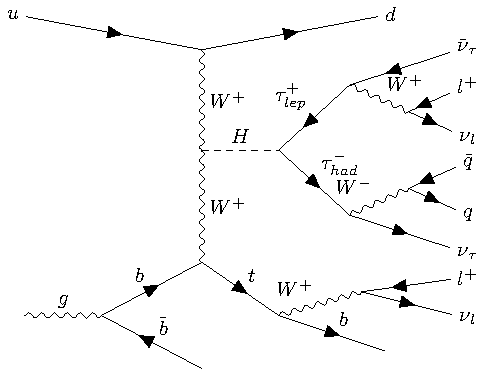
\includegraphics[width=\textwidth]{Feynman_diagrams/Feynman_DileptauGeneralRepresentative_dileptau_SS}
    \caption{\dilepSStau}
    \label{fig:tHq:intro:diltauFeynmanDiagram:SS}
  \end{subfigure}
  \hfill
  \begin{subfigure}[b]{0.45\textwidth}
    \centering
    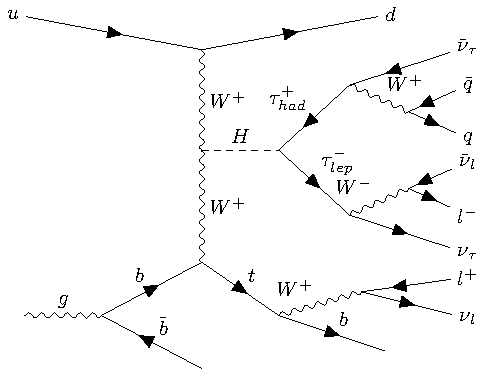
\includegraphics[width=\textwidth]{Feynman_diagrams/Feynman_DileptauGeneralRepresentative_dileptau_OS}
    \caption{\dilepOStau}
    \label{fig:tHq:intro:diltauFeynmanDiagram:OS}
  \end{subfigure}
  \caption{Representative LO Feynman diagrams (4FS) for the \tHq (\dileptau) in the $\PHiggs \rightarrow \tauhad \taulep$ decay channel 
  (dominant decay mode).
  Note that the two charged light-flavoured leptons in (a) have the same positive electrical 
  charge and in (b) these leptons have opposite charges.}
  \label{fig:tHq:intro:diltauFeynmanDiagram}
\end{figure}



%When assuming that one of the light-flavoured leptons is originated from the Higgs-boson decay
%and the other one from the top-quark decay, the determination of which lepton comes from which 
%particle is direct for the \dilepOStau but not for the \dilepSStau. 
%Since knowing the origin of the light-flavoured leptons can be very useful to define variables with
%the power to discriminate the \tHq signal from the background, tools are developed to associate 
%these leptons to its parent particles.

%- The fake rate estimates for light leptons and tau leptons are being checked to see if there is 
%anything that has to be treated differently for the two sub-channels.





%%%%%%%%%%%%%%%%%%%%%%
%           Data and simulated events          %
%%%%%%%%%%%%%%%%%%%%%%
\section{Data and simulated events }
\label{sec:ChaptH:Data_and_MC}
In this section the particularities of the data collected by the detector 
and the MC-simulated event samples are presented. The generalities 
of the data gathering and the production of the MC samples are
described in Chapter~\ref{chap:DataAndMC}.

% ~\cite{SgTopRun2NtuplesContents}
%~\cite{TOPQ}
All the search channels share the same object selection and use a common set of MC NTuples, which 
are produced with the SingleTopAnalysis\footnote{SingleTopAnalysis is
a ROOT-based software-package based on AnalysisTop. It is used to produce
NTuples. AnalsyisTop is the standard analysis software within Athena for Run 2 analysis 
in the Top Working Group.} using the TOPQ1 derivations %\footnote{The derivations were 
%introduced in Section~\ref{sec:Chap3.1:Data:Model}. The TopQ1 derivation \pablo{particularidad de topq1¿?}} 
as input. These TOPQ1 DAODs contain a single-lepton filter 
that requires at least one electron or muon that satisfies $|\eta| \leq 2.5$. %NTuples and derivations {sec:Chap3.1:Data:Model}
%need to satisfy one of the following requirements:
%\begin{itemize}
%	\item At least one electron with $\abseta \leq 2.5$ and \texttt{Electrons.DFCommonElectronsLHLoose}
%	\item Or at least one muon with $\abseta \leq 2.5$ and \texttt{Muons.muonType = 0} and \texttt{Muons.DFCommonGoodMuon}.
%\end{itemize}
Additionally, this lepton should have $\pT >20\,$GeV for 2015 data and above $25\,$GeV 
for both the 2016--2018 data and the MC simulations.
The produced NTuples have at least two \emu in their final state, one satisfying the condition above and
the other must present a  $\pT >10\,$GeV. %\pablo{Do these requirements account for the trigger sensitivity or why this?}

After the NTuples are generated with SingleTopAnalysis, a post-processing framework named \thqloop 
(Appendix~\ref{chap:Appendix:tHqLoop})
further manipulates the data samples to skim and slim\footnote{The slimming is done by removing 
unnecessary branches. In ROOT, a branch represents a variable associated with each event or entry in a TTree, which is a hierarchical data structure used for storing and analysing data in the ROOT framework.} them. 


%%%%%%%%%%%%%%%%%%%%%
%                    Data events                      %
%%%%%%%%%%%%%%%%%%%%%
\subsection{ATLAS-collected data samples}
\label{sec:ChaptH:Data_and_MC:Data}
The real-data samples used in this analysis correspond to the events
recorded by the ATLAS detector from $\Pproton\Pproton$ collisions with $25$~ns bunch spacing
delivered by the LHC at $\CM=13\,$TeV during Run 2. 
This corresponds to a total integrated luminosity of $L^{\text{Run 2}} = 140$~fb$^{-1}$ (see Section~\ref{sec:Chap3.1:Data:DeliveredLuminosity}).
The uncertainty corresponding to this integrated luminosity has been measured by the LUCID-2
detector to be $0.83\%$~\cite{ATLAS:2022hro, Avoni:2018iuv}. This data-taking period ranges from 2015 to 2018 and, for each year,
a different luminosity and uncertainty are measured, as is shown in Table~\ref{tab:ChaptH:Data:lumi}.
This data-taking period also presents different pile-up through the years. 
Figure~\ref{fig:Chap6:LHC:PileUp_15-18} presents the average number of interactions
in each crossing between proton bunches. As can be seen, the average pile-up increased
every year. 

%\begin{table}[h]
% \resizebox{\textwidth}{!}{\begin{tabular}{ccccc}
%    \toprule
%    Year & Periods & Run numbers & Number of events & Integrated luminosity (pb$^{-1})$ \\
%    \midrule
%    2015 & \dataperiodsFifteen & \datarunsFifteen & \dataeventsFifteen & \lumiFifteenInPbNoUnits\ $\pm$ \lumiFifteenRelUnc\% \\
%    2016 & \dataperiodsSixteen & \datarunsSixteen & \dataeventsSixteen & \lumiSixteenInPbNoUnits\ $\pm$ \lumiSixteenRelUnc\% \\
%    2017 & \dataperiodsSeventeen & \datarunsSeventeen & \dataeventsSeventeen & \lumiSeventeenInPbNoUnits\ $\pm$ \lumiSeventeenRelUnc\% \\
%    2018 & \dataperiodsEightteen & \datarunsEightteen & \dataeventsEightteen & \lumiEightteenInPbNoUnits\ $\pm$ \lumiEightteenRelUnc\% \\
%    \midrule
%   2015--2018 & All & \firstdatarunFifteen--\lastdatarunEightteen & \dataeventsAll & \lumiInPbNoUnits\ $\pm$ \lumiRelUnc\% \\
%    \bottomrule
%  \end{tabular}}
% \caption{Total integrated luminosity per year with their relative uncertainties for the Run 2.
%    Additionally, the data-taking periods, run numbers and number of events are shown for each year.}
%    \label{tab:ChaptH:Data:lumi}
%\end{table}

\begin{table}[h]
\centering
\resizebox{\textwidth}{!}{
\begin{tabular}{lllll}
\toprule
Year                                     							& 2015				& 2016 		& 2017 		& 2018 	\\ \midrule
Peak $\mathcal{L}(t)$ ($\times 10^{33}\,$\lumiunits)	& 5					& 13			& 16			& 19 		\\
Total delivered $L$ (fb$^{-1}$) 			& 4.0					& 38.5 		& 50.2 		& 63.4 \\
$L$ registered by ATLAS ($\text{pb}^{-1}$)	&$3244.54\pm1.13\%$ & $33402.2\pm0.89\%$ & $44630.6\pm1.13\%$ & $58791.6\pm1.10\%$  \\
Periods	& \dataperiodsFifteen& \dataperiodsSixteen & \dataperiodsSeventeen & \dataperiodsEightteen \\
Run numbers & \datarunsFifteen & \datarunsSixteen & \datarunsSeventeen & \datarunsEightteen \\
Number of events & \dataeventsFifteen & \dataeventsSixteen & \dataeventsSeventeen & \dataeventsEightteen \\
\bottomrule
\end{tabular}}
\caption{Peak luminosity, integrated luminosity delivered by the LHC and 
cumulative luminosity collected by the ATLAS detector at $\CM = 13\,$TeV during Run 2 per year~\cite{ATLAS:CONF:2019:021}}. 
%The uncertainties are measured with the LUCID-2 detector~\cite{ATLAS:2022hro, Avoni:2018iuv}.} 
\label{tab:ChaptH:Data:lumi}
\end{table}

\begin{figure}[h]
	\centering
 	 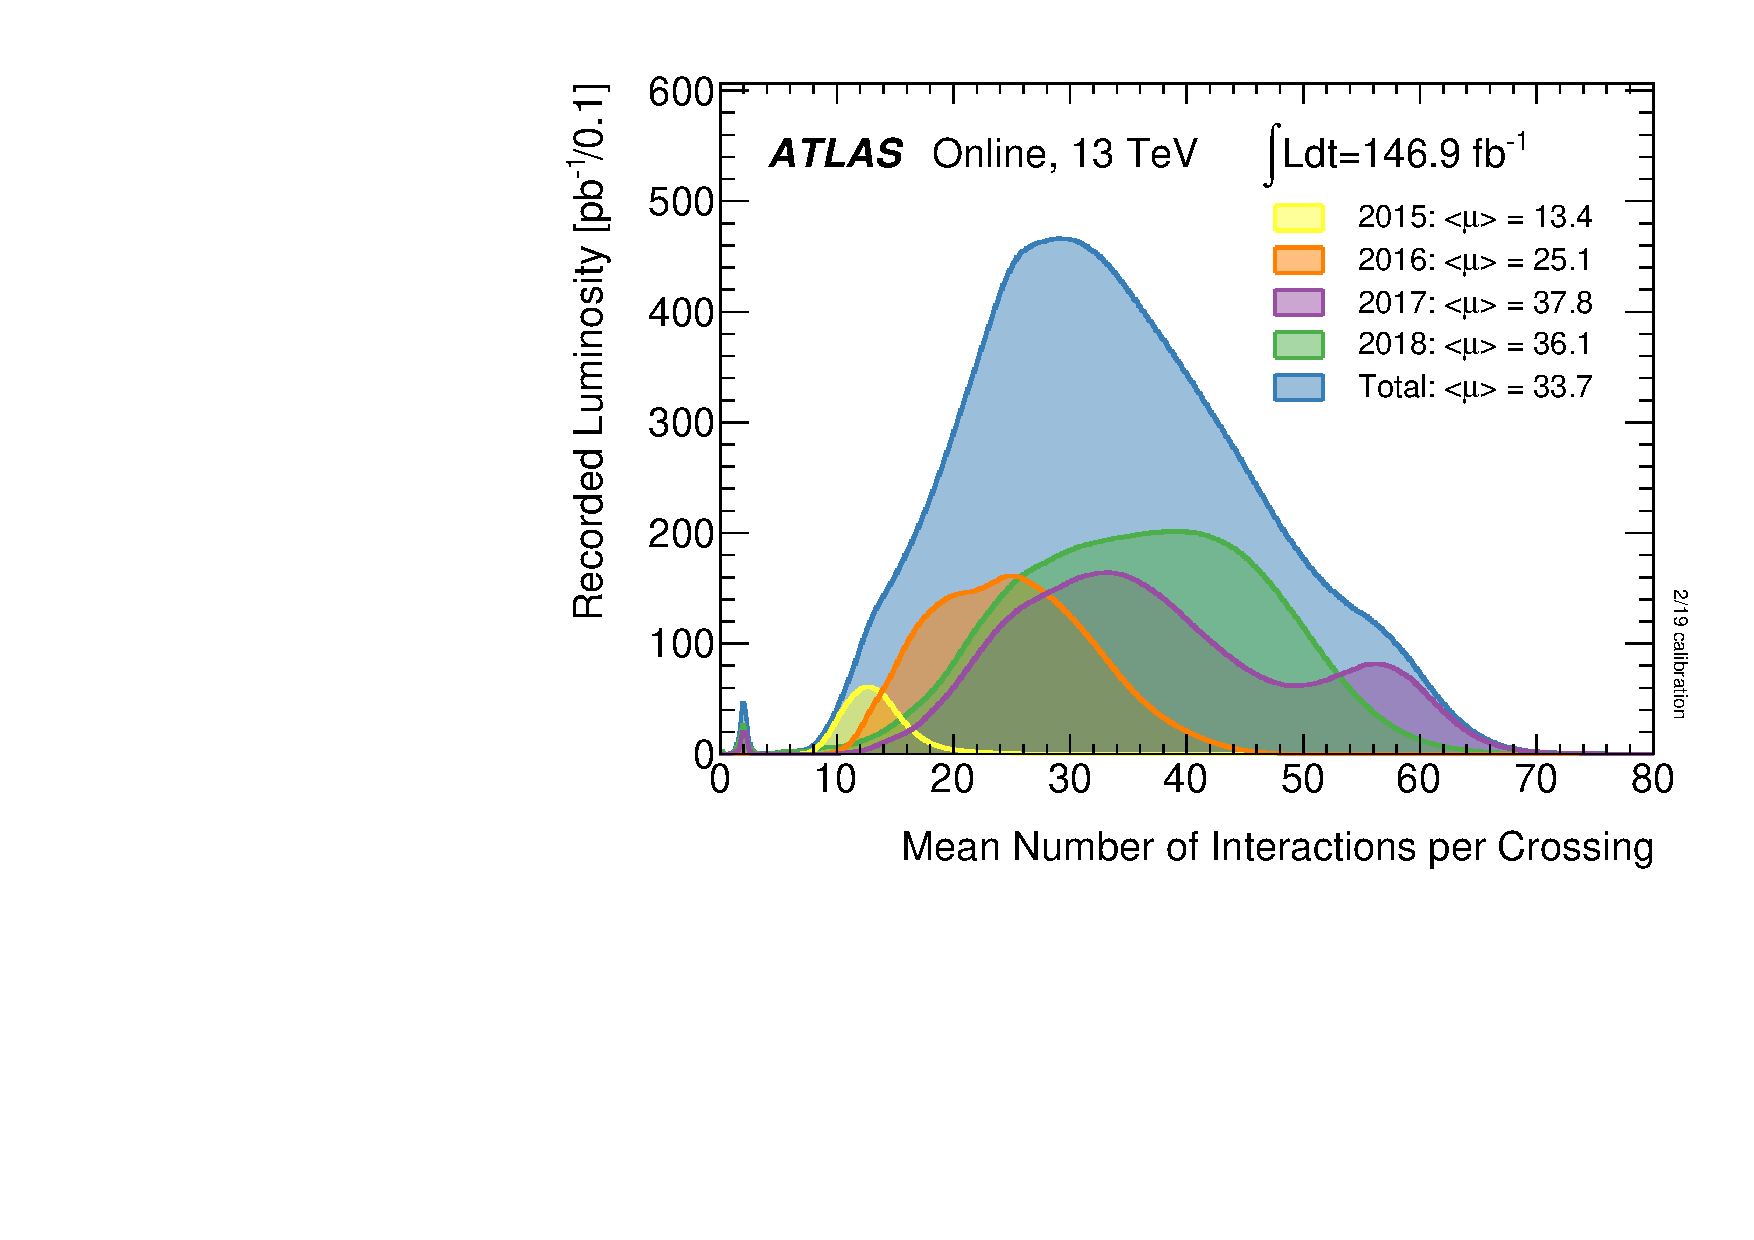
\includegraphics[width = 0.85\textwidth]{Chapter2/Pile-up_2015_2018}
	 \caption{Luminosity-weighted distribution of the mean number of interactions 
	 per crossing <$\mu$> for Run 2 in each year with $\Pproton \Pproton$ collisions data during stable beams at $\CM=13$~TeV~\cite{ATLAS:2022hro}.}
	\label{fig:Chap6:LHC:PileUp_15-18}
\end{figure}

As introduced in Section~\ref{sec:Chap3.1:Data:DeliveredLuminosity}, the GRLs is an xml file that selects the luminosity blocks that are considered good
to be used in an analysis. This is done by demanding that the LHC had stable beams and that all
the detectors and subdetectors were operating correctly.
The GRL has been used to filter the registered data at the luminosity blocks\footnote{A
luminosity block corresponds to about 1 or 2 minutes of data taking and has around $~10^{5}$ events. 
It is a unit of known luminosity.} level. %Source: https://indico.cern.ch/event/472469/contributions/1982677/attachments/1220934/1785823/intro_slides.pdf
Events were selected from a shared data stream using the unprescaled single-lepton triggers, 
which are detailed in Section~\ref{sec:ChaptH:ObjectDefReco:trigger}.


%%%%%%%%%%%%%%%%%%%%%
%                Simulated events                  %
%%%%%%%%%%%%%%%%%%%%%
\subsection{Simulated event samples}
\label{sec:ChaptH:Data_and_MC:MC}
The simulated event samples used in this analysis were produced using 
different MC-event generators and simulation frameworks. 
The generalities of the ATLAS simulation chain are described in 
Section~\ref{sec:Chap3.1:MC}.

The MC production is divided into campaigns, where the centre-of-mass energy,
geometry and conditions used in production correspond to a running period of
the LHC.  Three campaigns are used.
%Major campaigns align with calendar years, receiving names such as mc15 and mc16. 
%Meanwhile, minor-campaign versions often indicate updates or enhancements in 
%reconstruction software, trigger menus, or pile-up simulation and are denoted by 
%designations like mc15a, mc16b, and so on.
%The MC16a/d/e production campaigns are the employed ones in this analysis.
Various event generators interfaced with shower/hadronisation generators are used in this analysis. 

% PMG: Physics Modelling Group
% APG: ATLAS MC Production Group

\begin{comment} %Already explained in Chapter 4
After the event generation, the trigger and detector simulation are 
performed using the Athena.
The detector simulation is carried out either using the GEANT4 framework~\cite{GEANT4:2002zbu} 
for a detailed physics description or the \texttt{Atlfast2}~\cite{SOFT-2010-01} framework for 
faster simulation. The AFII strategy is used for the ATLAS
calorimeters, while GEANT4 is used for the rest of the simulation. 


The \pileup effect, is incorporated by overlaying the hard-scattering event 
with inelastic \pp\ events generated using \PYTHIA[8.186]~\cite{Sjostrand:2007gs}. 
The ATLAS third set of tuned parameters for minimum-bias events (A3 tune~\cite{ATL-PHYS-PUB-2016-017}) 
and the \NNPDF[2.3lo] set of PDFs~\cite{Ball:2012cx} are employed for the \pileup modelling.
\end{comment}

%Some generalities about the event simulation for this analysis are:
\begin{itemize}
	\item For the \pileup modelling (see Section~\ref{chap:DataAndMC:pileup}), \PYTHIA[8.186]
	is used with the ATLAS third set of tuned parameters for minimum-bias events 
	(A3 tune~\cite{ATL-PHYS-PUB-2016-017}) and the \NNPDF[2.3lo] set of PDFs~\cite{Ball:2012cx}.

	\item For the hard scattering process, unless it is specified differently, 
	the \NNPDF[3.0nlo]. PDF set is used.

	\item For the PS, unless explicitly stated otherwise, the \PYTHIA generator is used with 
	A14~\cite{ATL-PHYS-PUB-2014-021} tune and the \NNPDF[2.3lo] PDF set.
	
	\item The top-quark decay is simulated at LO using \MADSPIN~\cite{Frixione:2007vw, Artoisenet:2012st} 
	to preserve spin correlations, while the decay of the Higgs boson is generated either by \PYTHIA[8] 
	or \HERWIG[7] in the PS. 
	The decays of bottom and charm hadrons are simulated using either \EVTGEN[1.6.0] 
	or \EVTGEN[1.7.0]~\cite{Lange:2001uf}.

	\item	The MC-simulated events are weighted to match the distribution of the average 
	number of interactions per bunch crossing, \(\left<\mu \right>\), observed in the 
	real detector data. A rescaling factor of \(1.03\pm 0.04\) is applied 
	to the $\left<\mu \right>$ value of the samples to improve agreement between 
	data and simulation~\cite{STDM-2015-05}.% in the visible inelastic \pp\ cross-section\cite{STDM-2015-05}.
 
	\item	The FS event samples are used as the baseline whenever 
	available. For certain cases such as the \tHq signal process and the \tHW
	and four top-quark background processes, AFII event samples are used as baseline.
	Most of the systematic effects are evaluated using AFII samples, except for 
	specific systematic uncertainties such as \ttbar/\tW interference, \ttZ, \ttW, and \tWZ 
	modelling, where FS event samples are used. 
	The details about AFII and FS simulation strategies are
	provided in Section~\ref{sec:Chap3.1:MC:Steps:Reco}
\end{itemize}

These samples are used to assess efficiency and resolution models and to estimate 
systematic uncertainties. The details of each simulation event sample for each process 
are provided in the subsequent subsections.
 A summary of all \tHq signal and background processes 
is presented in Table~\ref{tab:ChaptH:Data_and_MC:MCsummary}. 
The relevance of the processes 
listed in Table~\ref{tab:ChaptH:Data_and_MC:MCsummary} is not uniform.
In this section, is is also discussed the significance of each background process, highlighting 
their respective importance and how it mimic the signal's final state. The estimation of the
background yields is presented in Section~\ref{sec:ChaptH:Bkg} 



%\pablo{En esa sección hay que explicar con detalle como se modela la señal y luego explicar también
%los principales fondos. El resto se ponen como minor backgrounds y se añade una tabla resumen de todos
%los procesos.}


\begin{table}[!htbp]  
  \begin{adjustbox}{max width=0.99\textwidth}
    \begin{tabular}{llllll}
      \toprule
      Process & Generator & Order (scheme) & PDF set & Parton shower & PDF set (tune) \\
      \midrule
      \multicolumn{6}{c}{Signal} \\
      \midrule
      \tHq & \MGNLO[2.6.2] & NLO (4FS) & \NNPDF[3.0nlo] nf4 & \PYTHIA[8.230] & \NNPDF[2.3lo] (A14 tune) \\
      \midrule
      \multicolumn{6}{c}{Backgrounds} \\
      \midrule
      \ttbar & \POWHEGBOX[v2] & NLO (5FS) & \NNPDF[3.0nlo] & \PYTHIA[8.230] & \NNPDF[2.3lo] (A14 tune) \\
      \(V\)+jets & \SHERPA[2.2.1] & NLO+LO & \NNPDF[3.0nnlo] & - & - \\
      \Diboson & \SHERPA[2.2.1-2] & NLO+LO & \NNPDF[3.0nnlo] & - & -\\
      \Triboson & \SHERPA[2.2.2] & NLO+LO & \NNPDF[3.0nnlo] & - & - \\
      \ttZ & \MGNLO[2.3.3] & NLO & \NNPDF[3.0nlo] & \PYTHIA[8.210] & \NNPDF[2.3lo] (A14 tune) \\
      \ttW & \SHERPA[2.2.10] & NLO & \NNPDF[3.0nnlo] & - & - \\
      %\ttV & \MGNLO[2.3.3] & NLO & \NNPDF[3.0nlo] & \PYTHIA[8.210] & \NNPDF[2.3lo] (A14 tune) \\
      \ttH & \POWHEGBOX[v2] & NLO (5FS) & \NNPDF[3.0nlo] & \PYTHIA[8.230] & \NNPDF[2.3lo] (A14 tune) \\
      \(t\)-channel & \POWHEGBOX[v2]  & NLO (4FS) & \NNPDF[3.0nlo] nf4 & \PYTHIA[8.230] & \NNPDF[2.3lo] (A14 tune) \\
      \Wt & \POWHEGBOX[v2] & NLO (5FS, DR) & \NNPDF[3.0nlo] & \PYTHIA[8.230] & \NNPDF[2.3lo] (A14 tune) \\
      \(s\)-channel & \POWHEGBOX[v2] & NLO & \NNPDF[3.0nlo] & \PYTHIA[8.230] & \NNPDF[2.3lo] (A14 tune) \\
      \tZq & \MGNLO[2.3.3] & NLO & \NNPDF[3.0nlo] & \PYTHIA[8.230] & \NNPDF[2.3lo] (A14 tune) \\
      \tHW{} & \MGNLO[2.8.1] & NLO (5FS, DR) & \NNPDF[3.0nlo] & \PYTHIA[8.245p3] & \NNPDF[2.3lo] (A14 tune) \\
      \tWZ & \MGNLO[2.3.3] & NLO & \NNPDF[3.0nlo] & \PYTHIA[8.212] & \NNPDF[2.3lo] (A14 tune) \\
      \ttt & \MGNLO[2.2.2] & NLO & \NNPDF[3.1nlo] & \PYTHIA[8.186] & \NNPDF[2.3lo] (A14 tune) \\
      \tttt & \MGNLO[2.3.3] & NLO & \NNPDF[3.1nlo] & \PYTHIA[8.230] & \NNPDF[2.3lo] (A14 tune) \\
      \ggH & \POWHEGBOX[v2] & NLO & \CT[10] & \PYTHIA[8.210] & \CTEQ[6L1] (\AZNLO tune) \\
      \qqH & \POWHEGBOX[v1] & NLO & \CT[10] & \PYTHIA[8.186] & \CTEQ[6L1] (\AZNLO tune) \\
      \WH & \PYTHIA[8.186] & LO & \NNPDF[2.3lo] & - & - \\
      \ZH & \PYTHIA[8.186] & LO & \NNPDF[2.3lo] & - & - \\
      \bottomrule
    \end{tabular}
  \end{adjustbox}
  \caption{Summary of the baseline-nominal-simulated signal and background event
    samples used in the \tHq analyses. The alternative simulations are described in Section~\ref{sec:ChaptH:Systematics:Theo}.}
  \label{tab:ChaptH:Data_and_MC:MCsummary}
\end{table}

%%%%%%%%%%%%%%%%%%%%%
%                Simulated signal                  %
%%%%%%%%%%%%%%%%%%%%%
\subsubsection{Simulated \tHq signal samples}
\label{sec:ChaptH:Data_and_MC:MC:Sig}
The \tHq event sample is generated using the \MGNLO[2.6.2]~\cite{Alwall:2014hca} 
generator at NLO, employing the \NNPDF[3.0nlo] nf4~\cite{Ball:2014uwa} PDF set. The 
$\mu_{\text{R}}$ and $\mu_{\text{F}}$ scales are set to a default scale 
based on $0.5\times \sum_{i}\sqrt{m_{i}^{2}+p_{\text{T}, i}^{2}}$, where 
$i$ runs over all the particles generated by the $\mathcal{M}$ calculation.
The simulation event samples are generated in the 4FS scheme (see Section 
\ref{sec:Chap1:Top:Production:SingleTop} for FS discussion). 
This is referred to as the nominal signal sample.
%the momenta of the particles generated from the matrix element calculation.


\begin{comment} % The inverted coupling testing is not on the scope of the document.
Additionally, samples of simulated \tHq signal events with the inverted Yukawa coupling 
hypothesis ($\yt=-1$) are produced using either the \MGNLO[2.6.2] and 
\MGNLO[2.8.1] generators at NLO with the \NNPDF[3.0nlo] nf4 PDF set, and interfaced 
with either \PYTHIA[8.230] or \PYTHIA[8.245], both using the A14 tune and the 
\NNPDF[2.3lo] PDF set. The $\mu_{\text{R}}$ and $\mu_{\text{F}}$ scales are also the same as for the nominal 
event sample.
\end{comment}

The normalisation of the \tHq signal samples is performed with respect to the
cross-section predictions obtained from NLO generator. 
For $\Pproton \Pproton$ collisions at
$\CM = \sqrt{13}\,$TeV, the cross-section of the ML channels 
corresponds to $\sigma_{\text{NLO}} (\tHq_{\text{ML}})= 16.7\,$pb
using a top-quark mass of $\mtop =172.5\,$GeV. %$\tHq (ML)$ refers
%to the multi-leptonic channels, in contrast to the $\tHq(\bbbar)$ with a cross section of 
%$\sigma(\tH(\bbbar))_{\text{NLO}} = 60.1\,$fb.
This cross-section is a factor 3.6 times smaller than the one for the $\tHq(\bbbar)$ production, 
with $\sigma_{\text{NLO}} (\tHq_{\bbbar})= 60.1\,$fb. 


%%%%%%%%%%%%%%%%%%%%%
%           Simulated background               %
%%%%%%%%%%%%%%%%%%%%%
\subsubsection{Simulated background samples}
\label{sec:ChaptH:Data_and_MC:MC:Bkg}
%%%%
%Define what background 
%%%%
The background can be defined as everything in a subset of the data that 
imitates the signal processes without truly being a signal event.  Therefore, 
in this study, whatever mimics the signature of an associated \tHq production 
with  \dileptau final state is referred to as background. 
%In other words, in this study, everything that is not the signal \tHq, is background.

%%%%
%Why is important to discriminate it. % http://www.thomasgmccarthy.com/an-introduction-to-collider-physics-ix
%%%%
To perform the physics analysis, it is fundamental to subtract the background events from the dataset
as much as possible to achieve higher signal purity.
By doing this, the analysed dataset resembles more to the process that is desired to study.
This procedure is the so called ``event selection'' and it is described in Section~\ref{sec:ChaptH:EventSelection}.

\begin{comment} % Already explained in Section 6.5
%%%%
% Classification in Reducible and Irreducible bkgs
%%%%
In our analysis, background events are classified into two distinct types:  
``reducible'' backgrounds and ``irreducible'' backgrounds.

Reducible backgrounds refer to situations where particles in the event 
simulation mimic the characteristics of the particles we are specifically 
interested in. For example, a high-energy electron can produce a signature 
that closely resembles that of a high-energy photon, leading to misidentification.

On the other hand, irreducible backgrounds involve physical objects that are of 
the same nature as the particles we are targeting. These backgrounds cannot be 
easily distinguished from our signal events based on their properties alone.

In the \dileptau channel, the dominant backgrounds consist of reducible events 
where jets misidentified as \tauhad are present. This is particularly observed in 
the \ttbar and \Zjets backgrounds. Additionally, other backgrounds include processes 
involving dibosons (VV) and \ttX production, such 
as \ttH, \ttZ, and \ttW.
\end{comment}

 
%In the \dileptau channel, the primary source of background arises from misidentified \tauhad. 
%Particularly, the cases where jets falsely resemble \tauhad signatures dominate this type of 
%misidentification. %This is further discussed in Section~\ref{sec:ChaptH:Bkg:Fakes}.
%While this type of backgrounds are discussed in Section~\ref{sec:ChaptH:Bkg:Fakes},
%the irreducible backgrounds are presented in Section~\ref{sec:ChaptH:Bkg:Irreducible}.


In the subsequent section, the MC simulation of the background processes 
is presented, highlighting their specific characteristics. Furthermore, an 
explanation is provided for each of these processes to clarify how they contribute
to the background. Later on, in Section~\ref{sec:ChaptH:Bkg}, a 
comprehensive description of the background estimation is discussed. %offering 
%detailed insights into the methodologies employed.

%\pablo{En estas subsecciones he de describir por qué cada uno de estos procesos es considerado como fondo. De qué forma imitan la signatura de \tHq.}

%%%%%
% ttbar %
%%%%%
\paragraph{Top-quark pairs}\mbox{}\\
The production of top-quark pair (\ttbar) events constitutes the main background source
for both \dileptau channels. Figure~\ref{fig:tHq:Backgrounds:Feynman_ttbar} presents
a \ttbar production Feynman diagram in which the top quarks decay leptonically. 
When these leptons are electrons or muons, the \ttbar process can mimic the
\dileptau signature if one of the quarks produces a jet that is wrongly reconstructed 
as a \tauhad. This background particularly relevant in the \dilepOStau channel, where
it surpasses the signal yields by three orders of magnitude.
As it is discussed in Section~\ref{sec:ChaptH:Bkg}, the misidentification of quarks as if they were \tauhad constitutes the main source of background.
If one of the leptons in the \ttbar diagram was a hadronically-decaying tau and the other an \emu, the 
\dileptau signature could be obtained if one of the \bjets is wrongly identified as an \emu. This second scenario
of misidentified \emu is less common but can still happen.

\begin{figure}[h]
\centering
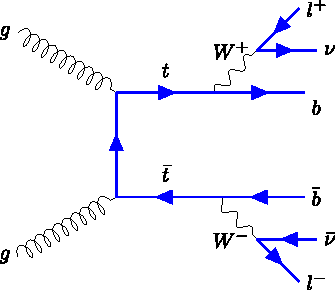
\includegraphics[width=.5\textwidth]{Feynman_diagrams/Vectorial_Backgrounds/Feynman_ttbar_Vectorial}
\caption{LO Feynman diagram for the \ttbar process, the main background. 
	In this particular diagram both \PW bosons decay leptonically.}
\label{fig:tHq:Backgrounds:Feynman_ttbar}
\end{figure}

%\pablo{The description of \ttbar generations seems too technical.}

Regarding its generation, the \ttbar events are simulated using 
\POWHEGBOX[v2]~\cite{Frixione:2007nw, Nason:2004rx, Frixione:2007vw, Alioli:2010xd}.
% which incorporates NLO  $\mathcal{M}$ in the strong coupling constant \alphas, and the \NNPDF[3.0nlo] PDF set~\cite{Ball:2014uwa}. 
The parameter \hdamp, controlling 
the matching between the \POWHEG generator and high-\pT radiation, is set to 
 $1.5$ the mass of the top quark~\cite{ATL-PHYS-PUB-2016-020}.
The $\mu_{\text{R}}$  and $\mu_{\text{F}}$ scales are set to the default scale of \(\sqrt{\mtop^{2} + \pT^{2}}\).
All these samples are generated in the 5FS.

% %%% Moved to generalities
%The subsequent PS and hadronisation processes are simulated using \PYTHIA[8.230], 
%adopting the A14 tune and the \NNPDF[2.3lo] PDF set. %In this context, the presented 
%analyses uses a non-all-hadronic filtered simulation sample with the dataset identifier 
%(DSID) 410470.
%The decays of bottom and charm hadrons are simulated using the \EVTGEN[1.6.0] program.


% %%% Moved to systematic
%The impact of using a different PS and hadronisation model is evaluated
%by comparing the nominal \ttbar sample with an event sample also produced with the
%\POWHEGBOX[v2] generator but interfaced with \HERWIG[7.13], using the
%\HERWIG[7.1] tune and the
%\MMHT[lo] PDF set. \POWHEGBOX provides $\mathcal{M}$ at NLO in the \alphas, and use the
%\NNPDF[3.0nlo] set of PDFs.  
%an \hdamp parameter value of $1.5$ times the mass of the top quark.

\begin{comment} % Explained in Section 6.7.2 :: Theoretical uncertainties
The uncertainty due to ISR is estimated 
by comparing the nominal \ttbar events using the A14 tune with \ttbar events with the same 
settings as the nominal ones, but employed the \texttt{Var3c up} or \texttt{down} variation 
of the A14 tune, which corresponds to the variation of \alphas for ISR in the A14 
tune~\cite{ATL-PHYS-PUB-2014-021}. The uncertainty due to FSR 
is evaluated by varying the $\mu_{\text{R}}$ scale for emissions from the PS up and down by a 
factor of two.
\end{comment}

The \ttbar sample is normalised to the cross-section prediction at NNLO
in QCD including the resummation of NNLL soft-gluon terms calculated using
\TOPpp[2.0]~\cite{Beneke:2011mq,Cacciari:2011hy,Baernreuther:2012ws,Czakon:2012zr,Czakon:2012pz,Czakon:2011xx}.
For \pp\ collisions at \(\rts = 13\,\)TeV, this cross-section corresponds to
\(\sigma_{\text{NNLO+NNLL}} (\ttbar)= 832 \pm 51\,\)fb using a top-quark mass of $\mtop = 172.5$~GeV.



%%%%%
% Zjets %
%%%%%
\paragraph{Single vector boson}\mbox{}\\
This background corresponds to the \Zjets and \Wjets productions, which are also referred
to as \(V\)+jets.
For \Zjets, represented in the Feynman diagram
 in Figure~\ref{fig:tHq:Backgrounds:Feynman_Zjets}, it can mimic the \dilepOStau
 signature when one of the \Pbottom-quark from the gluon splitting is misidentified as
 a \tauhad. Conforming, along with \ttbar the main background in that particular channel.
 
 
 \begin{figure}[h]
\centering
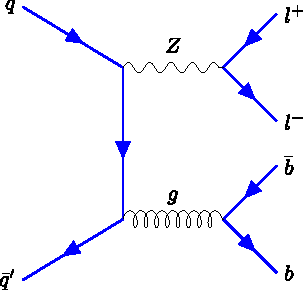
\includegraphics[width=.5\textwidth]{Feynman_diagrams/Vectorial_Backgrounds/Feynman_Zjets_Vectorial}
\caption{Representative LO Feynman diagram for the \Zjets process, the second most dominant background. In this particular case, the \PZ boson decays leptonically and
the gluon splits into a \bbbar pair.}
\label{fig:tHq:Backgrounds:Feynman_Zjets}
\end{figure}

The single-vector-boson processes are
simulated with \SHERPA[2.2.1] generator~\cite{Bothmann:2019yzt}. 
The $\mathcal{M}$ accuracy is NLO for up to two partons and LO for
up to four partons. 

The PS  is simulated with the default \SHERPA PS~\cite{Schumann:2007mg}, which is based on 
Catani--Seymour dipole factorisation and the cluster hadronisation model~\cite{Winter:2003tt}.
The $\mathcal{M}$ for a given jet multiplicity were matched to the PS using a colour-exact variant 
of the MC@NLO algorithm~\cite{Hoeche:2011fd}.  
The $V$+jets samples are normalised to a NNLO
prediction~\cite{Anastasiou:2003ds}.

%%%%%
% ttV %
%%%%%
\paragraph{Top-quark pair in association with a single vector boson}\mbox{}\\
Right after the single-boson and \ttbar processes, the \ttV processes (i.e. \ttZ and \ttW)
are the most relevant backgrounds. Particularly in the \dilepSStau channel, the two \ttV
productions are among the four most relevant backgrounds. 

There are various ways in which this process can mimic the final state of the signal.
For instance, for the \ttZ production depicted in the Feynman diagram in 
Figure~\ref{fig:tHq:Backgrounds:Feynman_ttZ}, the \dileptau signature can be
reproduced in two ways. Either if one and only one of the charged leptons is a \tauhad or
if one of the jets from the top decay is misidentified as a \tauhad and one of the light leptons
is not detected.

%After the top quarks decay through the \tWb vertex, there are three vector bosons. If the
%\PZ and one \PW boson decay leptonically and the other \PW boson does it hadronically,  
%there will three charged leptons in the final state.
If one of these leptons is a \tauhad and the other two are either electrons or muons, the
final-state objects are those of the \dileptau.

\begin{figure}[h]
\centering
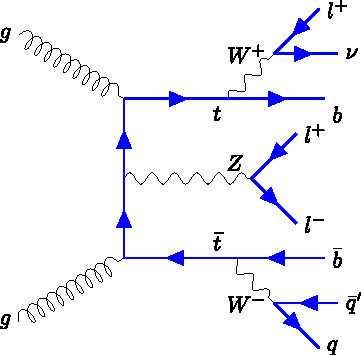
\includegraphics[width=.5\textwidth]{Feynman_diagrams/Vectorial_Backgrounds/Feynman_tt+X_Vectorial}
\caption{Representative LO Feynman diagram for the \ttZ with the \PZ boson decaying leptonically, one of the top 
quarks is decaying leptonically and the other hadronically. }
\label{fig:tHq:Backgrounds:Feynman_ttZ}
\end{figure}


The \ttW events are simulated using the \SHERPA[2.2.10] generator at 
NLO accuracy in QCD with the \NNPDF[3.0nnlo] PDF collection.
This framework incorporates a strategy that merges multiple legs, 
allowing for the integration of one extra parton at NLO and two at LO.
 An event-by-event correction factor was applied to this sample
that provide virtual NLO EWK corrections. 
Additionally, a simulation sample at LO accuracy in
QCD was also generated with \SHERPA[2.2.10] but for the \ttWj final state to emulate
EW corrections to \ttW production.
The generation of \ttZ events event is conducted with 
the \MGNLO. %[2.3.3]~\cite{Alwall:2014hca} generator, providind $\mathcal{M}$ at
%NLO in \alphas and using the \NNPDF[3.0nlo] PDF set. 

The \muR and \muF scales are set to the default of \(0.5 \times \sum_i \sqrt{m^2_i+p^2_{\text{T},i}}\),
where the sum runs over all the particles generated from the  $\mathcal{M}$ calculation.
%Top quarks undergo LO decay viag \MADSPIN to preserve spin correlations. These events 
%are then processed with \PYTHIA[8.210] for the PS and hadronisation, using the A14 tune 
%and the \NNPDF[2.3lo] PDF set. The \EVTGEN[1.2.0] program simulates the decays of 
%bottom and charm hadrons.


%%%%%%%
% ttH %
%%%%%%%
\paragraph{Top-quark pair in association with a Higgs-boson }\mbox{}\\
The \ttH process is discussed in depth in Section~\ref{sec:Chap1:ttH}.
If the Higgs boson and one of the top quarks decay to leptons
and the other top quark to $\Pquark\APquark$, the multiplicity in leptons
of the \dileptau channel is reproduced and the \ttH is reconstructed 
as a \tHq process. The mimicking of the signal process can also
take place by other decay modes of the \ttH if a quark-initiated jet
is misidentified as a \tauhad.
This background is particularly important in the \dilepSStau channel.

To simulate the \ttH processes, the \POWHEGBOX[v2] generator with the \NNPDF[3.0nlo] PDF set
is used. The functional form of the $\mu_{\text{R}}$ and $\mu_{\text{F}}$ scales was
set to \(\sqrt[3]{m_\text{T}(t)\cdot m_\text{T}(\bar{t}) \cdot m_\text{T}(H)}\), 
where $m_\text{T}$ is the transverse mass.
%The events were interfaced to \PYTHIA[8.230]~\cite{Sjostrand:2014zea}
%using the A14 tune and the
%\NNPDF[2.3lo] PDF set. The decays of bottom and charm hadrons
%were performed by \EVTGEN[1.6.0].
 
At $\CM=13$~TeV, the cross-section is computed to NLO QCD and 
NLO EW precision with \MGNLO~\cite{LHCHiggsCrossSectionWorkingGroup:2016ypw} and it
is $\sigma_{\text{NLO QCD + NLO EW}}^{\texttt{pred}} (\ttH) = 507^{+35}_{-50}$~fb.
The uncertainties correspond to variations of \alphas and the \muR and \muF scales.
 
%%%%%%%
% Diboson %
%%%%% %%
\paragraph{Diboson}\mbox{}\\
The diboson background is one of the most dominant after \ttbar and \Zjets
but its presence is one order of magnitude smaller. % Figure~\ref{fig:tHq:Backgrounds:Feynman_Diboson}
%presents the Feynman diagrams for these two processes.
In the case of the $\PW\PZ$ diboson process (see Feynman diagram in
Figure~\ref{fig:tHq:Backgrounds:Feynman_Diboson:WZ}), there
are three leptons in the final state and, hence, the object multiplicity
of the \dileptau channel can be replicated without any type of misidentification.
For the $\PZ\PZ$ diboson process (see Feynman diagram in
Figure~\ref{fig:tHq:Backgrounds:Feynman_Diboson:ZZ}), there
are four leptons and, therefore, one of them should not be reconstructed
to mimic the \dileptau signature.

\begin{figure}[h]
\centering
\begin{subfigure}[b]{0.45\textwidth}
   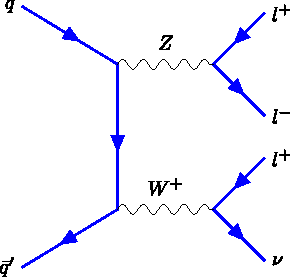
\includegraphics[width=1\linewidth]{Feynman_diagrams/Vectorial_Backgrounds/Feynman_Diboson_ZW_Vectorial}
   \caption{$\PW \PZ$}
   \label{fig:tHq:Backgrounds:Feynman_Diboson:WZ}
\end{subfigure}
\begin{subfigure}[b]{0.45\textwidth}
   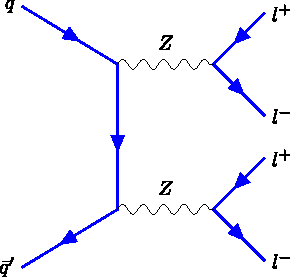
\includegraphics[width=1\linewidth]{Feynman_diagrams/Vectorial_Backgrounds/Feynman_Diboson_ZZ_Vectorial}
   \caption{$\PZ \PZ$}
   \label{fig:tHq:Backgrounds:Feynman_Diboson:ZZ}
\end{subfigure}
\caption{Representative LO Feynman diagram for the diboson processes. 
	In these diagrams, all vector bosons are decaying leptonically.}
\label{fig:tHq:Backgrounds:Feynman_Diboson}
\end{figure}


Samples of \diboson final states (\(VV\)) are simulated with the
\SHERPA[2.2.1] or 2.2.2 generator depending on the process.
The samples use  $\mathcal{M}$s at NLO accuracy in QCD.
The \NNPDF[3.0nnlo] set of PDFs is used~\cite{Ball:2014uwa}, along with the
dedicated set of tuned PS parameters developed by the
\SHERPA authors.



%%%%%%%%%%
% single top quark %
%%%%%%%%%%%
\paragraph{Single-top-quark processes}\mbox{}\\
The three single-top-quark productions described in Section~\ref{sec:Chap1:Top:Production:SingleTop}
are simulated but only the \tW production plays a relevant role.  In the \dilepOStau channel, 
\tW stands out as a significant background, but its impact is not as significant as \ttbar and \Zjets.
All three single-top-quark processes are modelled using \POWHEGBOX[v2]
generator in conjunction with \PYTHIA[8]. Although some of the \tW and \tchannel samples 
use \POWHER[7]. 


%%%%%%%
%      tX      %
%%%%%%%
\paragraph{Single-top quark in association with a boson}\mbox{}\\
Another family of background processes is the \tX, which is composed
by \tZq, \tWZ and \tWH. In Figure~\ref{fig:tHq:Backgrounds:Feynman_tX},
the Feynman diagrams for \tZq and \tWZ are presented and
in Section~\ref{sec:Chap1:tH:ProductionModes} the \tWH production mode
receives detailed attention. %While none of these three processes is very dominating in terms of
%event yields, their distinct characteristics render them noteworthy for analytical consideration.

The \tWH process exhibits heightened sensitivity to deviations of \yt from the SM expectation
and a more inclusive \tH search has to include this process as part of the signal.
The \tZq production presents a challenge due to its close resemblance to the \tHq signal.
When stringent selection requirements are applied to 
discriminate the signal from all the background processes, the reduction of \tZq is considerably 
more modest compared to other processes.

\begin{figure}[h]
\centering
\begin{subfigure}[b]{0.47\textwidth}
   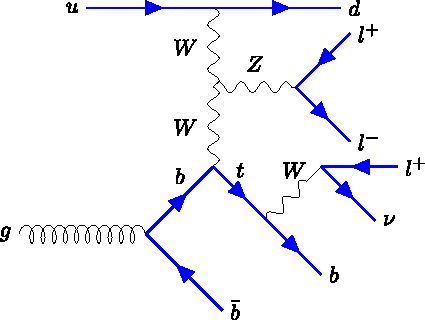
\includegraphics[width=1\linewidth]{Feynman_diagrams/Vectorial_Backgrounds/Feynman_tZq_Vectorial}
   \caption{\tZq}
   \label{fig:tHq:Backgrounds:Feynman_Diboson:tZq}
\end{subfigure}
\begin{subfigure}[b]{0.52\textwidth}
   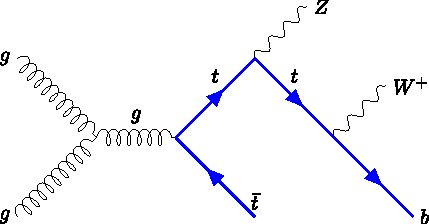
\includegraphics[width=1\linewidth]{Feynman_diagrams/Vectorial_Backgrounds/Feynman_tWZ_Vectorial}
   \caption{\tWZ}
   \label{fig:tHq:Backgrounds:Feynman_Diboson:tWZ}
\end{subfigure}
\caption{Representative LO Feynman diagrams for the \tZq and \tWZ productions.
The \tZq process has the exact same final state as a \tHq production.
The \tWZ can replicate the lepton multiplicity of the \tHq process if 
the \PW and \PZ bosons decay leptonically.} %Also, if the \PZ boson decays to
%two light leptons and the hadronically decaying \PW boson is misidentified with 
%a \tauhad.}
\label{fig:tHq:Backgrounds:Feynman_tX}
\end{figure}

\subparagraph{\tHW{} process}
The \tHW events are generated at NLO in the 5FS using \MGNLO[2.8.1]
with the \NNPDF[3.0nlo]. %The events are interfaced with
%\PYTHIA[8.245p3] using the A14 tune and the \NNPDF[2.3lo] PDF set.
The functional form of the \muR and \muF scales is set to the
default scale \(0.5\times \sum_i \sqrt{m^2_i+p^2_{\text{T},i}}\), where the sum runs over
all the particles generated from the $\mathcal{M}$ calculation.
The DR scheme is employed to handle the interference
between \tHW{} and \ttH.
%The decays of bottom and charm hadrons are simulated
%using the \EVTGEN[1.7.0] program


\subparagraph{\tZq process}
Using \MGNLO[2.3.3], the \tZq sample is simulated at NLO. % with the \NNPDF[3.0nlo] PDF set
%and then interfaced with \PYTHIA[8.230] using the A14 tune
%and the \NNPDF[2.3lo] PDF set.
%The top-quark decay is simulated at LO with \MADSPIN to preserve spin correlations.
Using the 4FS,  the functional form of the \muR and \muF scales
is set to $4\sqrt{m_{\Pbottom}^2+ p^{2}_{\text{T},b}}$, where $m_{\Pbottom}$ is the mass of
the $m_{\Pbottom}$-type quark~\cite{Frederix:2012dh}.
%The decays of bottom and charm hadrons were simulated using the \EVTGEN program~\cite{Lange:2001uf}.

\subparagraph{\tWZ process}
The \tWZ processes are simulated at NLO in the 5FS using \MGNLO[2.3.3]. %with the \NNPDF[3.0nlo] PDF set.
%The events are interfaced with \PYTHIA[8.212].  using the A14 tune and the \NNPDF[2.3lo] PDF set.
The top quark and the \PZ boson are decayed at LO using \MADSPIN. Here, the decay 
of the \PZ boson is restricted to a pair of charged leptons.
The \muR and \muF scales are set to the top-quark mass.
To address the  interference between \tWZ and \ttZ, the DR scheme is employed.
%The decays of bottom and charm hadrons were simulated using the
%\EVTGEN[1.2.0].

\paragraph{Non-dominant processes}\mbox{}\\
Other minor backgrounds considered in this analysis are the triboson ($VVV$), 
the Higgs-boson processes ($\Pgluon\Pgluon$F, VBH, VH), three top quark ($t$$t$$t$)
and four top quarks ($\ttbar$$\ttbar$). The simulation procedure of the baseline samples for all these 
processes is summarised in Table~\ref{tab:ChaptH:Data_and_MC:MCsummary}.


%The underlying event is generally done with Pythia8 in ATLAS. In the tHq samples we used \MGNLO for the calculation of the matrix element and \PYTHIA[8] for the hadronisation and parton showering. We are also working on alternative samples with \Herwig[7] as parton shower generator.
%\pablo{While in section 3 I describe how the events and samples are generally generated and simulated, in this section I should describe what is specifically used in this analysis}




%%%%%%%%%%%%%%%%%%%%%%%%%%
%           Object definition and reconstruction         %
%%%%%%%%%%%%%%%%%%%%%%%%%%
\section{Object definition}
\label{sec:ChaptH:ObjectDefReco}
In Chapter~\ref{chap:ObjectReconstruction}, a general overview of the object 
reconstruction process is provided. Different possible definitions for the 
physical objects are discussed in that chapter. 
In contrast, this section focuses on presenting the 
specific definitions employed for this analysis at hand.


%The \antikt algorithm with a radius parameter of \(R=0.4\) is used to reconstruct jets with a four-momentum recombination scheme, using \topos as inputs. Jet energy is calibrated to the hadronic scale with the effect of \pileup removed

%Hadronic jets are reconstructed from calibrated three-dimensional \topos.
%Clusters are constructed from calorimeter cells that are grouped together using a topological clustering algorithm.
%These objects provide a three-dimensional representation of energy depositions in the calorimeter and implement a nearest-neighbour noise suppression algorithm.
%The resulting \topos are classified as either EM or hadronic based on their shape, depth and energy density.
%Energy corrections are then applied to the clusters in order to calibrate them to the appropriate energy scale for their classification.
%These corrections are collectively referred to as \textit{local cluster weighting}, or LCW, and jets that are calibrated using this procedure are referred to as LCW jets~\cite{PERF-2012-01}.}

%
% Triggers
%
\subsection{Triggers}
\label{sec:ChaptH:ObjectDefReco:trigger}
To select events from collisions, a two-level-trigger-system is employed, as documented in Reference~\cite{TRIG-2016-01} and 
described in Section~\ref{sec:Chap2:Trigger_and_DAQ}. 
%To reduce the rate of accepted events, first the L1 trigger operates through hardware
%and, secondly, the software-based trigger HLT further reduces the acceptance. 
%The L1 operates through hardware and utilises partial detector information to decrease the rate of accepted events from 
%the interaction frequency of $40\,$MHz to $100\,$kHz. The HLT, on the other hand, is software-based and accepts 
%events at a rate of $1\,$kHz.
During the data-taking period spanning 2015--2018, varying pile-up conditions necessitated the use of different single-lepton 
(electron or muon) triggers. % which were not subjected to prescaling~\cite{LowestUnprescaled}. The trigger names employed 
%in this analysis are listed in Table~\ref{tab:ChaptH:ObjectDefReco:Triggers}. These triggers are combined using a logical 
%\texttt{OR} operation.
These triggers are combined using the logical \texttt{OR} operator:

%% Commenting this because it is too technical 
\begin{comment}

\begin{table}[!htbp]
  \begin{adjustbox}{max width=0.99\textwidth}
    \begin{tabular}{c|ll}
      \toprule
      Year & Single-electron trigger & Single-muon trigger \\
      \midrule
           & \texttt{HLT\_e24\_lhmedium\_L1EM20VH} & \texttt{HLT\_mu20\_iloose\_L1MU15} \\
      \datafirstyear\ & \texttt{HLT\_e60\_lhmedium} & \texttt{HLT\_mu50} \\
           & \texttt{HLT\_e120\_lhloose} & \\
      \midrule
           & \texttt{HLT\_e26\_lhtight\_nod0\_ivarloose} & \texttt{HLT\_mu26\_ivarmedium} \\
      2016--\datalastyear\ & \texttt{HLT\_e60\_lhmedium\_nod0} & \texttt{HLT\_mu50} \\
           & \texttt{HLT\_e140\_lhloose\_nod0} & \\
      \bottomrule
    \end{tabular}
  \end{adjustbox}
    \caption{Employed single-lepton trigger depending on the light-lepton flavour and year.
    %These individual single-lepton triggers are combined using a logical \texttt{OR} operation
    }
  \label{tab:ChaptH:ObjectDefReco:Triggers}
\end{table}
% https://twiki.cern.ch/twiki/bin/view/AtlasProtected/TopqTriggers
% https://twiki.cern.ch/twiki/bin/viewauth/Atlas/TrigGlobalEfficiencyCorrectionTool#Supported_trigger_combinations



%Electron triggers
The electron triggers in this analysis employ a selection criteria that involves matching a calorimeter cluster to a track. 
Subsequently, electrons are required to meet identification criteria utilising a multi-variate technique with a likelihood discriminant.
Depending on the year, the single-electron triggers used in this analysis are as follows:
\begin{itemize}
	\item In \datafirstyear, electron triggering involved requiring a transverse energy deposit (\ET) above $20\,$GeV at the L1. 
	At the HLT, the full-calorimeter granularity and tracking information were considered, and the reconstructed-calorimeter
	cluster was matched to a track. The trigger electron object was required to be isolated, with a \texttt{medium}-identification
	requirement  and have $\ET > 24\,$GeV.
	As commented in Section~\ref{sec:ChaptH:ObjectDefReco:electron}, the \texttt{tight}, 
	\texttt{medium} and \texttt{loose} categories correspond to the different working points (WP) of the
	likelihood-based algorithm for prompt-electron identification and non-prompt electron rejection.
	See References~\cite{ATLAS:2019jvq, ATLAS:2019qmc} for more details about the likelihood identification.
	
	\item In the years 2016--2018, the electron triggers required electrons to satisfy a \texttt{tight} identification at the HLT, 
	along with an isolation criterion, and have an $\ET > 26\,$GeV.
	
	\item Two complementary triggers were employed throughout Run$\,$2 to mitigate efficiency losses at high \pT, 
	in addition to the previous triggers. These triggers either selected \texttt{medium} electrons with $\ET > 60\,$GeV 
	at the HLT or selected \texttt{loose} electrons with $\ET > 120\,$GeV in 2015 and 
	$\ET > 140\,$GeV in 2016--2018. 
	%The By \texttt{loose} its meant that no isolation requirements were demanded.
\end{itemize}

%Muon triggers
Muons in this analysis are triggered by matching tracks reconstructed in both the MS and ID.
In \datafirstyear, the muon triggers required muons to satisfy a \texttt{loose}-isolation requirement and
have a \pT greater than $20\,$GeV. In the years 2016--2018, the isolation criterion was tightened, 
and the threshold was increased to $\pT > 26\,$GeV. The isolation criteria uses 
Similar to the electron triggers, to mitigate efficiency losses due to isolation at high \pT, an additional 
muon trigger without any isolation requirement was available throughout all these years. 
This trigger selected \texttt{loose}-isolated muons with $\pT > 50\,$GeV. 
\end{comment}

%% Versión corta del triggering para el análisis.
\begin{itemize}
	\item The single-electron triggers rely on the likelihood-based algorithm for prompt-electron 
	identification and non-prompt electron rejection described in Section~\ref{sec:ChaptH:ObjectDefReco:electron}.
	Isolation and identification requirements are applied as well.  
	Besides, various lower transverse energy (\ET) thresholds ranging from 20~GeV to 26~GeV 
	are applied for low-\pT electrons. 
	For high-\pT electrons, two additional complementary triggers with lower-\ET thresholds 
	from 60~GeV to 140~GeV are employed. 
	
	\item Muons in this analysis are triggered by matching tracks reconstructed in both the MS and ID,
	along with isolation criteria. Similar to the electron triggers, to mitigate efficiency losses due to 
	isolation at high \pT, several lower-\pT thresholds from 20~GeV to 50~GeV are set.
\end{itemize}




%
% Electrons
%
\subsection{Electrons}
\label{sec:ChaptH:ObjectDefReco:electron}
%Electron candidates in this analysis are identified using energy deposits in the ECAL that correlate with a track in ID.
%From these clusters, a likelihood-based algorithm for electron identification is
%used to differentiate prompt electrons from non-prompt lepton~\cite{ATLAS:2019jvq, ATLAS:2019qmc}. %~\cite~{PERF-2017-01,EGAM-2018-01}
%This method classifies electrons into three categories based on identification efficiency:
%\texttt{tight}, \texttt{medium}, and \texttt{loose}. The looser is the identification efficiency,
%the more electrons are accepted but the purity of prompt leptons is lower. 

In this analysis, the electron candidates must meet several criteria: 
they should have a \pT greater than 10~GeV, be within the pseudorapidity range of $|\eta^\mathrm{clust}| < 2.47$, 
and pass the \texttt{tight} identification level.  
Electron candidates are excluded if their calorimeter clusters lie within the transition region 
between the barrel and the end-cap sections of the EM calorimeter, defined as 
$1.37 < |\eta^\mathrm{clust}| < 1.52$. 
Additionally, these electrons must pass an isolation test based on the ``Prompt Lepton Improved Veto'' 
(PLImprovedTight) isolation working point~\cite{ATLAS:2022swp}.
 This isolation working point uses a multivariate analysis technique, combining shower shape and 
 track information, to effectively differentiate between prompt electrons and those that arise from 
 backgrounds such as hadronic jets, photon conversions, or the decay of heavy-flavour hadrons.

Additionally, the associated track must satisfy  $|\zzsth| < 0.5\,$mm 
and $|\dzero| / \sigma(\dzero) < 5$. Here, $z_{0}$ represents the longitudinal impact 
parameter relative to the reconstructed primary vertex, where the primary vertex is 
defined as the vertex with the highest scalar sum of the squared transverse-momenta 
of associated tracks with $\pt > 500\,$MeV. The \dzero corresponds to the transverse-impact 
parameter relative to the beam axis, and $\sigma(\dzero)$ denotes the uncertainty on \dzero.

%~\cite{twiki-ECIDS}
%~\cite{twiki-elAmbiguity}
In certain analysis regions, additional requirements are imposed on electrons. 
These include the application of 
the \texttt{Electron Charge ID Selector Tool} (ECIDS),
a BDT-based tool which enhances the rejection of electrons 
with misidentified-electrical charges. Another tool referred to as
\texttt{Electron Ambiguity Tool} is used to suppress the misidentification of 
photons reconstructed as electrons.

\begin{comment}
The requirements for preselected electrons used in the overlap-removal process\footnote{The 
overleap removal vetoes physical objects in the event with reconstruction ambiguities that can lead 
to double-counting.  It is described in Section~\ref{sec:ChaptH:ObjectDefReco:OverlapRemoval}.}
and electrons selected for this analysis are summarised in left column of 
the Table~\ref{tab:ChaptH:ObjectDefReco:Electrons_Muons}.
The recommendation is the use of likelihood-based electron identification 
techniques~\cite{PERF-2017-01,EGAM-2018-01} due to their improved 
background rejection compared to cut-based electron identification. 
Different WPs are supported, which correspond to different levels 
of efficiency in identifying prompt electrons and rejection of non-prompt electrons. 
For pre-selected electrons, a \texttt{looseAndBLayerLH} identification is applied.
%On the other hand, for electrons selected in one of the analysis regions, a \texttt{tightLH} 
%identification is required.
These electrons must satisfy the following criteria: $\pT > 10,$GeV and $|\eta| < 2.47$. 
Additionally, a requirement on electron isolation is imposed, which corresponds to the 
\texttt{PLImprovedTight} (Prompt Lepton Improved Veto) isolation working 
point~\cite{ATLAS:2022swp}. This isolation WP is defined by a %Hyneman:2672803, DeVivieDeRegie:2256658
multivariate likelihood discriminant that combines shower shape and track information 
to distinguish prompt electrons from electron candidates originating from hadronic jets, 
photon conversions, and decays of heavy-flavour hadrons.
%~\cite{twiki-IFF,twiki-ISOWP,PLIV}

The reconstructed track associated with the electron must satisfy: $|\zzsth| < 0.5\,$mm 
and $|\dzero| / \sigma(\dzero) < 5$. Here, $z_{0}$ represents the longitudinal impact 
parameter relative to the reconstructed primary vertex, where the primary vertex is 
defined as the vertex with the highest scalar sum of the squared transverse-momenta 
of associated tracks with $\pt > 400\,$MeV. \dzero corresponds to the transverse impact 
parameter relative to the beam axis, and $\sigma(\dzero)$ denotes the uncertainty on \dzero.
Electron candidates are excluded if their calorimeter clusters lie within the transition region 
between the barrel and the endcap of the EM calorimeter, defined as 
$1.37 < |\eta^\mathrm{clust}| < 1.52$. To account for the efficiency differences between data 
and simulation when applying these requirements, associated scale factors (SFs) for electron 
reconstruction, identification, and isolation are applied in Monte Carlo (MC) simulations~\cite{egammaRecommendations}.

In certain analysis regions, additional requirements are imposed on electrons. These include the application of 
the ``Electron Charge ID Selector Tool'' (ECIDS)~\cite{twiki-ECIDS}, which enhances the rejection of electrons 
with misidentified electrical charges. Moreover, for specific regions, cuts on the \texttt{DFCommonAddAmbiguity} 
and \texttt{ambiguityType} variables are implemented, as defined by the ``Electron Ambiguity Tool'' in 
the E/gamma derivation framework~\cite{twiki-elAmbiguity}. These cuts are designed to suppress the contribution 
from electrons originating from photon conversions by removing objects with multiple reconstructed tracks in close 
proximity to the calorimeter cluster.
It is worth noting that the requirement ``$\texttt{ambiguityType} = 0$'' in conjunction 
with ``$\texttt{DFCommonAddAmbiguity} \leq 0$'' signifies the selection of electrons with a 
veto on internal/material photon conversion candidates. In the following discussion, this will be referred 
to as the ``$e/\gamma$ ambiguity-cuts''.

\pablo{The information in subSection~\ref{sec:ChaptH:ObjectDefReco:electron} has been taken from the int-note. Maybe it is too technical.}
\end{comment}

%
% Muons
%
\subsection{Muons}
\label{sec:ChaptH:ObjectDefReco:muon}
The preselected-muon candidates used for the overlap-removal process must satisfy $\pt > 7$~GeV, $|\eta| < 2.5$, 
and pass the \texttt{medium} identification criteria. %~\cite{MCPRecommendations}.
This WP imposes conditions on the number of hits in the ID and MS subsystems, as well as 
on the significance of the charge-to-momentum ratio~\cite{ATLAS:2016lqx, ATLAS:2020auj}. %PERF-2015-10, MUON-2018-03

Isolation criteria are established using the level of isolation determined by a multivariate likelihood algorithm.
These requirements (\texttt{tight}) are applied to suppress 
contributions from misidentified or non-prompt muons~\cite{ATLAS:2022swp}. %Hyneman:2672803, DeVivieDeRegie:2256658

Moreover, the track associated with the muon candidates must satisfy the recommended 
cuts for the longitudinal impact parameter and transverse 
impact parameter (d0). The reconstructed track must satisfy $|\zzsth| < 0.5\,$mm and $|\dzero| / \sigma(\dzero) < 3$. 

A summary of the specific-object-definition criteria for electrons and muons is presented in Table~\ref{tab:ChaptH:ObjectDefReco:Electrons_Muons}.

\begin{comment}
The selection criteria for muons are summarised in the right column of Table~\ref{tab:ChaptH:ObjectDefReco:Electrons_Muons}.
Following the recommendations, preselected muons used for the overlap-removal process must satisfy: $\pt > 10$~GeV, $|\eta| < 2.5$, 
and the \texttt{medium} identification criteria. %~\cite{MCPRecommendations}. 
This \texttt{medium}-WP imposes conditions on the number of hits in the ID and MS subsystems, as well as 
on the significance of the charge-to-momentum ratio ($q/p$)~\cite{PERF-2015-10, MUON-2018-03,twiki-MuonSelection}. 
If a muon is flagged as ``bad' due to insufficient momentum resolution, the entire event is removed,
following the recommendations~\cite{twiki-MuonSelection}.
In addition to the criteria for preselected muons, muons selected for analysis regions are subject 
to the \texttt{PLImprovedTight} isolation requirement. This isolation criterion is applied to suppress 
contributions from misidentified or non-prompt muons~\cite{ATLAS:2022swp, ATLAS:2016lqx}. %Hyneman:2672803, DeVivieDeRegie:2256658

The recommended cuts for the longitudinal impact parameter and transverse 
impact parameter (d0) are applied to muon candidates. The reconstructed track 
associated with the muon must satisfy $|\zzsth| < 0.5\,$mm and $|\dzero| / \sigma(\dzero) < 3$. 
SFs for muon identification and isolation are applied as multiplicative factors to the MC-event weight. 
These SFs correct for the differences in efficiency between data and MC simulations. 
The details of these corrections can be found in the References~\cite{PERF-2015-10}.
% impact parameter (IP)
% transverse impact parameter (d0)

\begin{table}[!htbp]
  \begin{tabular}{ l|l|l }
    \toprule
    & \multicolumn{1}{c|}{Pre-selected electron} & \multicolumn{1}{c}{Pre-selected muon} \\
    \midrule
    Identification   & \multicolumn{1}{c|}{\texttt{looseAndBLayerLH}} & \multicolumn{1}{c}{\texttt{medium}} \\
    Acceptance       & $\pt > 10\,$GeV, $|\eta^\mathrm{clust}| < 2.47$  & $\pt > 10\,$GeV, $\abseta < 2.5$ \\
                     &  except $1.37 < |\eta^\mathrm{clust}| < 1.52$          & \\
    Impact parameter & $|\dzero/\sigma(\dzero)| < 5.0$                   & $|\dzero/\sigma(\dzero)| < 3.0$ \\
                     & $|\zzsth| < 0.5\,$mm                      & $|\zzsth| < 0.5\,$mm \\
     Overlap removal & \multicolumn{2}{c}{See Section~\ref{sec:ChaptH:ObjectDefReco:OverlapRemoval}} \\
    \bottomrule
    & \multicolumn{1}{c|}{Electron} & \multicolumn{1}{c}{Muon} \\
    \midrule
    Identification   & \multicolumn{1}{c|}{\texttt{tightLH}} &  \multicolumn{1}{c}{\texttt{medium}}\\
    Isolation        & \texttt{PLImprovedTight}  & \texttt{PLImprovedTight} \\
    Extra selections & ECIDS, $e/\gam$ ambiguity-cuts &  \\
    \bottomrule
  \end{tabular}
  \caption{Summary of the electron and muon object definitions. The selection requirements for actual
          electrons/muons are applied in addition to the pre-selected objects used for the overlap removal 
          (Section~\ref{sec:ChaptH:ObjectDefReco:OverlapRemoval}).}
   \label{tab:ChaptH:ObjectDefReco:Electrons_Muons}. %% Too technical table. Better use a simplified one.
\end{table}
\end{comment}

\begin{table}[!htbp]
  \begin{tabular}{ l|l|l }
    \toprule
    & \multicolumn{1}{c|}{Electron} & \multicolumn{1}{c}{Muon} \\
    \midrule
    Identification  & \multicolumn{1}{c|}{\texttt{tight}} &  \multicolumn{1}{c}{\texttt{medium}}\\
    Isolation         & \multicolumn{1}{c|}{\texttt{tight}}  & \multicolumn{1}{c|}{\texttt{tight}} \\
    Acceptance    & $\pt > 10\,$GeV, $|\eta^\mathrm{clust}| < 2.47$  & $\pt > 10\,$GeV, $\abseta < 2.5$ \\
                     &  except $1.37 < |\eta^\mathrm{clust}| < 1.52$          & \\
    Impact parameter & $|\dzero/\sigma(\dzero)| < 5.0$                   & $|\dzero/\sigma(\dzero)| < 3.0$ \\
                     & $|\zzsth| < 0.5\,$mm                      & $|\zzsth| < 0.5\,$mm \\
    
    Extra selections & ECIDS, $e/\gam$ ambiguity-cuts &  \\
    \midrule
    Overlap removal & \multicolumn{2}{c}{See Section~\ref{sec:ChaptH:ObjectDefReco:OverlapRemoval}} \\

    \bottomrule
  \end{tabular}
  \caption{Summary of the electron- and muon-object definitions uses in this analysis.}
   \label{tab:ChaptH:ObjectDefReco:Electrons_Muons} % Simplified version
\end{table}


%
% Hadronic taus
%~\cite{TauRecommendations}
\subsection{Hadronically-decaying taus}
\label{sec:ChaptH:ObjectDefReco:tau}
The selection criteria for \tauhad candidates are outlined in Table~\ref{tab:ChaptH:ObjectDefReco:Tau} 
and adhere to the guidelines established by the Tau CP group~\cite{ATLAS:2015boj, ATLAS:2019uhp}. 
The \tauhad objects must satisfy the criteria of $\pt > 20\,$GeV, $\abseta < 2.5$, excluding the range 
$1.37 < |\eta^\mathrm{clust}| < 1.52$, and have either 1 or 3 associated tracks. 
This requirement is applied because, as mentioned in Section~\ref{sec:Chap3:Reco:Tau}, the \Ptau-leptons
decay to one or three prongs.
To distinguish \tauhad candidates from other objects, they must pass the \texttt{medium (loose)} JetID 
requirement, which is defined using a RNN, as well as fail the cut 
on the electron BDT. No specific veto is applied for muons. The energy calibration is performed using 
the MVA Tau Energy Scale (MVA TES) method.
Scale factors for taus are applied to 
account for efficiency and energy scale corrections. %as outlined in~\cite{TauRecommendations},


\begin{table}[!htbp]
\centering
  \begin{tabular}{l|l}
    \toprule
      & \multicolumn{1}{c}{\tauhad} \\
    \midrule
    Acceptance     & $\pt > 20\,$GeV, $|\eta^\mathrm{clust}| < 2.5$   \\
                    &  except $1.37 < |\eta^\mathrm{clust}| < 1.52$         \\
    Number of tracks & 1 or 3\\
    Identification & \texttt{RNN Medium (Loose)} \\
    Electron veto  & \texttt{electron BDT Loose (Loose)}   \\
    Overlap removal      & See Section~\ref{sec:ChaptH:ObjectDefReco:OverlapRemoval} \\
    \bottomrule
  \end{tabular}
    \caption{Summary of the \tauhad object definitions with the loose criteria in parentheses.
  The selection requirements for actual \tauhad are applied in addition to the pre-selected objects used for the overlap removal.}
  \label{tab:ChaptH:ObjectDefReco:Tau}
\end{table}

%
% jets
%
\subsection{Jets}
\label{sec:ChaptH:ObjectDefReco:jets}

%~\cite{JVT}
%~\cite{JVT-WP}
Jets are reconstructed using the anti-$k_t$ jet algorithm~\cite{Cacciari:2008gp} on particle-flow 
objects~\cite{PERF-2015-09}, with a distance parameter of $R = 0.4$, implemented in 
the \Fastjet package~\cite{Fastjet} (referred to as \texttt{AntiKt4EMPFlowJets} jet collection)\footnote{The
jet reconstruction is performed using the \antikt algorithm with a radius parameter of \(R=0.4\). 
The reconstruction process involves a four-momentum recombination scheme, where the input consists of particle-flow objects.
Jet energy is calibrated to the hadronic scale with the effect of \pileup removed.}. 
The Jet Vertex Tagger (JVT)~\cite{ATLAS-CONF-2014-018,PERF-2014-03}, recommended by 
the Jet/\met CP group, is used to select jets. Jets are retained if they have $\pt > 20\,$GeV 
and fall within the pseudorapidity range of $\abseta < 4.5$. Additionally, jets with $\pt < 60\,$GeV 
and $\abseta < 2.4$ must satisfy $\JVT > 0.5$ to meet the criteria of the \texttt{Tight} JVT WP. 
For forward jets with $2.5 < \abseta < 4.5$ and $\pt < 120\,$GeV, an alternative \JVT WP (\fJVT) 
is applied, requiring $\fJVT < 0.4$ along with a timing requirement on the jet~\cite{ATLAS-CONF-2014-018}. %~\cite{ATLAS:2014cva}. 
The jet definition and \btag requirements are summarised in Table~\ref{tab:jetsdef}. 

The jet calibration procedure follows the standard method recommended by the Jet/\met CP group, 
which corrects the jet energy to match, on average, the true jet energy at the particle level and applies 
in-situ corrections for data~\cite{JETM-2018-05}. 


%Concerning the jets, the EMPFlow algorithm is used.

%bjets
\subsubsection{Identification of \btagged jets}
\label{sec:ChaptH:ObjectDefReco:bjets}
%Various algorithms exploit the decay properties of \ensuremath{b\text{-hadrons}} to perform 
%jet flavour identification. Their generalities are described in Section~\ref{sec:Chap3:Reco:Bjets}.
In this study, the \texttt{DL1r} algorithm, a MVA method for \btag, 
is employed~\cite{ATL-PHYS-PUB-2015-039,ATL-PHYS-PUB-2017-013,ATL-PHYS-PUB-2017-003} (see Section~\ref{sec:Chap3:Reco:Bjets}). 
%The \texttt{DL1r} tagger combines information from the impact parameters of displaced tracks 
%and the topological properties of secondary- and tertiary-decay vertices reconstructed within the 
%jet to identify \bjets. 
The jets are \btagged if the values of the \texttt{DL1r} discriminant exceed certain 
thresholds or WPs. Four WPs are defined for the \texttt{DL1r} tagger, 
corresponding to selecting 85\%, 77\%, 70\%, and 60\% of \bjets in \ttbar simulated events. 
To assess the \btag performance comprehensively, the efficiency of the \texttt{DL1r} tagger is 
measured using collision data. The \texttt{DL1r} tagger discriminant is
defined in Equation~\ref{eq:Chap3:DL1r_discriminant}.


\begin{table}[htbp]
\centering
  \begin{tabular}{l|l}
    \toprule
    \multicolumn{2}{ c }{Pre-selected jet}\\
    \midrule
    Collection         & \multicolumn{1}{c}{\texttt{AntiKt4EMPFlowJets}} \\
    Acceptance         & $\pt > 20\,$GeV, $\abseta < 4.5$ \\
    Jet Vertex Tagger  &  $\JVT > 0.5$ if  $\abseta < 2.4$ and  $\pt < 60\,$GeV \\
                       &  $\fJVT < 0.4$ if $2.5 < \abseta < 4.5$ and $\pt < 120\,$GeV \\
    Overlap removal    & See Section~\ref{sec:ChaptH:ObjectDefReco:OverlapRemoval} \\
    \bottomrule
    \multicolumn{2}{c}{\btag jet}\\
    \midrule
    Acceptance     & $\pt > 20\,$GeV, $\abseta  < 2.5$ \\
    \btag    &  \texttt{DL1r} algorithm \\
    \bottomrule
  \end{tabular}
    \caption{Summary of the jet selection criteria and \btag.}
  \label{tab:jetsdef}
\end{table}


%
% overlap removal
%
\subsection{Overlap removal}
\label{sec:ChaptH:ObjectDefReco:OverlapRemoval}

Once all the objects are identified, to avoid that a single signature 
is identified as different physical objects, the overlap removal is applied, as
Section~\ref{sec:Chap3:Reco:OverlapRemoval} introduced.
To avoid the double-counting, in this analysis, the pre-selected \texttt{Loose} 
leptons and jets are used. Then, the following steps are applied to resolve
the ambiguities: %~\cite{OR}
\begin{enumerate}
  \item Any electron found with a track overlapping with any other electron is removed. 
  	The electron is also removed if it shares a track with a muon (except if it is a calorimeter muon) since the
  	electron object is very likely to be identified from the tracks that the muon produced in the ID.

  \item Any calorimeter muon (see Section~\ref{sec:Chap3:Reco:Mu}) found to share a track with an electron is removed.
  	This measure is taken because calorimeter muons objects are reconstructed in the region where the MS is not
	fully instrumented. 
  %\item Any electron found to share a track with a muon is removed.
  \item Any jet found within a $\Delta R \leq 0.2$ of an electron is removed, as it is very possible that the jet corresponds to the electron.
  \item Any electron subsequently found within $\Delta R \leq 0.4$ of a jet is removed in order to
  	reduce the impact of non-prompt electrons.
  \item Any jet with fewer than 3 tracks associated to it found within $\Delta R \leq 0.2$ of a muon is removed.
  	This is done to reduce the number of fake jets  from muons depositing energy in the calorimeters.
  %\item Any jet with fewer than 3 tracks associated to it, which has a muon ID track ghost-associated to it, is removed.
  %	This is done to reduce the number of fake jet  from muons depositing energy in the calorimeters.
  \item Any muon subsequently found within $\Delta R \leq 0.4$ of a jet is removed to reduce the 
  	contribution from muons from heavy-flavour decays within a jet.
  \item Any \tauhad found within a $\Delta R \leq 0.2$ of an electron is removed.
  \item Any \tauhad found within a $\Delta R \leq 0.2$ of any type of muon is removed.
  	If the tau has $\pt > 50\,$GeV, it will only be removed if it is found to overlap with a combined-type muon.
  \item Any jet found within a $\Delta R \leq 0.2$ of a \tauhad is removed.
\end{enumerate}
The overlap removal procedure is implemented by applying the criteria in the order specified.%in the \enquote{harmonised} option in the \texttt{AssociationUtils} package~\cite{OR}.

%
%MET
%
\subsection{Missing transverse momentum}
The $\overrightarrow{E}_{T}^{miss}$ is reconstructed by summing the 
negative vector of transverse momenta (\pT) of reconstructed and calibrated particles and 
jets (referred to as hard objects) after performing the overlap removal. 
Additionally, a soft term is included, which consists of charged-particle tracks associated 
with the hard scatter vertex~\cite{PERF-2016-07, ATLAS-CONF-2018-023}. The purpose of
the soft term is to account for low-momentum particles that may not be identified among the 
final state objects~\cite{PERF-2011-07, PERF-2014-04, ATL-PHYS-PUB-2015-027}. 
The \MET serves as a measurement of the undetectable particles in an event and is subject to 
energy losses caused by detector inefficiencies, acceptance limitations, and energy resolution.
In this analysis, the main source of \MET are the neutrinos in the final state.

%%%%%%%%%%%%%
%           Signal              %
%%%%%%%%%%%%%
\section{Signal}
\label{sec:ChaptH:Sig}
In this section, a study on some of the signal properties is presented.
First of all the generation of the truth-level information of the \tHq processes
is presented in Section~\ref{sec:ChaptH:Sig:truth}. Later, the method to 
determine the parent particle for the light leptons in the \dilepSStau channel
is presented in Section~\ref{sec:ChaptH:Sig:LepAsign}. Finally, the reconstruction
of the kinematic properties of the Higgs boson and the top quark is discussed 
in Section~\ref{sec:ChaptH:Sig:EventReconstruction}.
It is interesting to note how each of these studies needs the previous one, i.e.
the reconstruction of the signal process needs the leptons assignment, and
the lepton association uses the truth-level information.


%In this section, it is discussed how it is find what we know as signal. In a particular study, the ``signal''
%is the set of events in the dataset that correspond to the process of interest. Therefore, in this case, the 
%signal is composed by \tHq production events with a \dileptau  final state. In contrast, the background 
%processes are those which, a priori, look like the signal process but it is not. A more detailed definition 
%of what a background is and how it is classified can be found in Section~\ref{sec:ChaptH:Bkg}.

  % xsec ranges - the challenge in tHq searches 
%As mentioned already, the \tHq cross-section is very small. 
%One of the big challenges of LHC is the wide range of cross sections that
%of the different process that take place there. When the cross section
%is huge, the process is typically uninteresting. When it is large the process
%is already known. The medium cross-sections corresponds to not-so-well
%studied process, and when it is low is for process yet to be discovered.
%This causes that the main backgrounds are much larger than the signal,
%swamping the interesting physics with known processes. Therefore, in order
%to produce some small number of signal events, it is necessary to also produce
%so many of uninteresting ones that they even happen in the same crossing (pile-up).
%\pablo{Maybe this paragraph can be put somewhere else or removed}
%paragraph source: https://indico.ific.uv.es/event/6735/contributions/19450/attachments/10615/14389/higgs_cpan_nov22.pdf


%\subsection{Signal generation and validation}
%\label{sec:ChaptH:Sig:GenerationValidation}
%\pablo{rivet <- Esto lo puso Carlos en el esqueleto que sugirió}

\subsection{Validation of parton-level simulations}
\label{sec:ChaptH:Sig:truth}
As already presented in Section~\ref{sec:Chap3.1:MC:Steps}, the parton-level 
information refers to the MC-generated events before taking into account
the effects of the interaction of the particles with the matter of the detector. It also includes
the PS and hadronisation information. The parton-level-simulation information is kept in the 
reconstructed MC sample and can be matched to reconstructed objects.

In the ATLAS top-quark-physics group, a dedicated software package 
is used analyse, administrate and store the parton-level information. 
This package is referred to as \texttt{TopPartons}. %~\cite{TopPartonsGitLab}
The kinematic information and the 
true identity\footnote{Identity refers to which particle it is.
 The identity is commonly referred to as PDG-ID, which is the particle 
 numbering scheme defined by the Particle Data Group. 
It assigns a unique code to each type of particle. 
For instance, PDG-ID(\PHiggs boson)$ = 25$ 
and PDG-ID(\Ptop quark)$ = 6$.} of each of the particles 
in the event is saved in the NTuples through this library. The scripts to address
the \tHq events within \texttt{TopPartons} had to be developed and validated in
pursuance of having proper parton-level information.
In order to confirm the correct performance of the whole software, 
theoretical calculations have to be carried and compared
to the output of the program.    
In Appendix~\ref{chap:Appendix:TopPartons} the details of this task are discussed
in detail. First, in Section~\ref{sec:ChaptH:Sig:truth:TopPartons}, the details
of how the parton-level is included in the \texttt{TopPartons}-software package are
given. Secondly, in Section~\ref{sec:ChaptH:Sig:truth:Calculations}, we present the calculations
performed to determine the fractions in which each Higgs-boson-decay channel 
contributes to the \dileptau final state. Note that this development is not done only
for the \dileptau channel but for all ML channels. 

From the calculations in Section~\ref{sec:ChaptH:Sig:truth:Calculations} it
is deducted that from all \tHq events considered in the ML searches,
only a $3.72\%$ decay into a \dileptau final state. %  dileptau = 3.715767739%
From these, as can be seen in Table~\ref{tab:ChaptH:TruthSummary}, 
more than in 80\% of cases the \tauhad is produced in
the Higgs-boson-decay chain. 

\begin{table}[h]
\centering
\begin{tabular}{l|ll|l}
\toprule
       \multicolumn{1}{c|}{Higgs-boson decay} 	& \multicolumn{2}{c|}{Origin of \tauhad} &    \multirow{2}{*}{Total}     \\ \cline{2-3}
      \multicolumn{1}{c|}{channel}  		& Top quark        				& Higgs boson       &   \\ \midrule
\Htautau 	& 5.06      					& 64.06        		      			& 69.13	\\
\HWW    	& 9.01         				& 18.01              				& 27.02 	\\
\HZZ    	& 2.22          				& 1.64               				& 3.85   	\\ 
\midrule
Total  	& 16.29           				& 83.71              				& 100.00 	\\
\bottomrule
\end{tabular}
%	OLD RESULTS
%	\Htautau 	& 6.96    					& 88.11        		      			& 95.07  \\
%	\HWW    	& 1.41         				& 2.82              					& 4.23  \\ 
%	\HZZ    	& 0.40          				& 0.297               				& 0.70   \\ \midrule
%	Total  	& 8.78           				& 91.22              				& 100.00 \\
\caption{Contribution as a percentage of each Higgs-boson decay channel to the \dileptau final state obtained
from calculations combining the BRs of the considered decays.
Here is also presented whether the \tauhad is generated from the top quark or the Higgs-boson decay chain.
The discrepancies with the first row of Table~\ref{tab:ChaptH:tHqChannelsYields} are due to the reconstruction efficiency 
and selection requirements.}
\label{tab:ChaptH:TruthSummary}
\end{table}



Having a proper parton-level information is fundamental for this analysis because it is
used in several different tasks: from the determination of the light-lepton origin in
the \dilepSStau channel to the estimation of the \tauhad-misidentification contribution. 

\subsubsection{Comparison between software and calculation results}
With all decay scenarios incorporated into the \texttt{TopPartons} code, and having
calculated from the expected production fractions, the last step to validate the
parton-level simulations is two compare these two elements and ensure that
they are consistent.
%The last step to validate the code developed for the parton-level information
%is to contrast the output of \texttt{TopPartons} to the theoretical calculations and check that
%both are in agreement.
The metric used to perform the comparison is the ratio between the \tHq(\dileptau) event yields
 in a particular Higgs-boson-decay channel and all the events in that particular decay mode:  %particular decay-mode

\begin{equation*}
    \frac{\text{Number of events}(H \rightarrow \text{Decay channel} \rightarrow  \dileptau)}{\text{Number of events}(H \rightarrow \text{Decay channel)}}\, .
\end{equation*}

In Table~\ref{tab:ChaptH:Prediction_VS_TopPartons}, the BR-based calculations
performed in Section~\ref{sec:ChaptH:Sig:truth:Calculations} are put alongside 
the results of the parton-level truth informations described in Section~\ref{sec:ChaptH:Sig:truth:TopPartons}.
As can be seen, the agreement between the calculations and the \texttt{TopPartons} output is resonable for
the two main Higgs-boson-decay channels. For these, the disagreement is of 1.2\% for the $\Ptau\Ptau$  and 
5.9\% for the $\PW \PW$. 
In contrast, a discrepancy of 60\% is found in the $\PZ \PZ$ decay mode. 
The origin of the variance in the $\PZ \PZ$ decay is not due to bungs in the code
that generates the parton-level information. Instead, it is originated from the omission
of certain configurations in the $\PZ \PZ$ decay mode within the evaluation tool.
Even though the conflict in $\PZ \PZ$ is much larger than for the other channels, this is not so problematic
since the \HZZ accounts for a very small part of the total \tHq events in the \dileptau final-state channel  (3.86\%). 


\begin{table}[h]
\centering
\begin{tabular}{l|l|l}
\toprule
Yields ratio								&   Calculation   	& \texttt{TopPartons} result \\
\midrule
$\frac{\Htautau \rightarrow \dileptau }{\Htautau}$  	&   0.1246         	&  $0.1232  \pm 0.0057$ 	\\ 
$\frac{\HWW 	\rightarrow \dileptau}{\HWW}$       	&   0.0141        		&  $0.0151  \pm 0.0009$   \\ 
$\frac{\HZZ 	\rightarrow \dileptau }{\HZZ}$           	&   0.0164         	&  $0.0100  \pm 0.002$     \\ \bottomrule
% \textbf{$3l$}                & \textbf{Prediction} & \textbf{Result} \\ \hline
%$H \rightarrow WW \rightarrow SR(3l) / H \rightarrow WW$                &   0.0162         &  $0.0169  \pm 0.0010$      \\ \hline
%$H \rightarrow \tau \tau \rightarrow SR(3l) / H \rightarrow \tau \tau$  &   0.0314         &  $0.0271  \pm 0.0027$     \\ \hline
%$H \rightarrow ZZ \rightarrow SR(3l) / H \rightarrow ZZ$                &   0.0325         &  $0.0152  \pm 0.0031$      \\ \hline
\end{tabular}
\caption{Theoretical predictions compared to the \texttt{TopPartons} output. 
The uncertainty on the second column corresponds to the statistical error. }
% both the count and errors are computed with  the event weights.
\label{tab:ChaptH:Prediction_VS_TopPartons}
\end{table}

%\FloatBarrier 


%%%%%%%%%%%%%%%%%%%
%           Lepton-origin assignment    %
%%%%%%%%%%%%%%%%%%%
\subsection{Light-lepton-origin assignment}
\label{sec:ChaptH:Sig:LepAsign}
% Importance
The two light leptons in the final state of the \dileptau channel can originate either from the 
Higgs boson or the top quark. The ambiguities regarding the origin of these light-flavoured
leptons make the reconstruction of the top-quark and Higgs-boson systems extremely difficult.
Nevertheless, the electric charge of these leptons could provide useful information to probe their origins.

To know whether the light-flavoured leptons in the final state are originated from
the Higgs boson or the top quark is very beneficial to both reconstruct the event and
design variables at reconstruction level with high discriminant power. As shown in 
Sections~\ref{sec:ChaptH:EventSelection:SR} and \ref{sec:ChaptH:EventSelection:CR},
the variables using the lepton assignment information play a relevant role not only in 
the definition of the signal-enriched section but also the in the determination of 
 the control regions (see Section~\ref{sec:ChaptH:EventSelection:CR}) to constrain the most important background processes.

According to the calculations performed by combining the BR of the Higgs boson, the top quark 
and all its decay products (see Section~\ref{sec:ChaptH:Sig:truth}),
in the \dileptau channel of \tHq production, the \tauhad is produced 83.7\% of times as a 
product of the Higgs-boson decay in opposition to the 16\% in which it comes from the top-quark
disintegration. 

\paragraph{Origin association for \dilepOStau}\mbox{}\\ %opposite-sign leptons
In the dominant scenario (\tauhad originated from the Higgs-boson system) the association of which light-flavoured
lepton comes from the top-quark decay and which one comes from the Higgs-boson decay can be
done directly if these two leptons have opposite electric charges, i.e. in the \dilepOStau channel.
Since the Higgs boson is neutrally charged, the sum of the charge of its decay products should be zero. Therefore,
in the \dilepOStau channel, while the light lepton with opposite charge to that of the \tauhad is the one coming
from the Higgs boson, the other lepton, i.e. the one with the same charge as \tauhad, is the one originated 
from the top-quark decay.



\paragraph{Origin association for \dilepSStau}\mbox{}\\ %same-sign leptons
In contrast to the \dilepOStau channel, in the case of \tauhad coming from the Higgs boson,
 when the two light leptons have the same electric charge, \dilepSStau,
it is not possible to know, a priori, which of the leptons comes from the top-quark system and which 
from the Higgs-boson decay.  
%All of this, assuming that the \tauhad comes from the Higgs boson, otherwise,
%if the \tauhad was produced as a decay product from the top, it would not make sense 
%to talk about the lepton origin since both light leptons would be associated to the Higgs system.

To perform this association for the \dilepSStau three methods %relying in the truth-level information
are tested. These are: %\pablo{Igual no vale la pena mencionar los otros porque tampoco se entienden bien}
\begin{itemize}
	\item \textbf{Initial approach}:  A NN based on the Keras framework 
	was trained to perform the assignment task~\cite{Walther:2743809}. 
	In labelling the data, it was assumed 
	that the leading lepton ($\ell_{1}$) always originates from the top quark. Truth-level studies have 
	shown that in most cases, the lepton coming from the decay chain of the top quark 
	is the leading lepton. This is because the top quark typically carries more momentum 
	than the Higgs boson. However, it should be noted that this assumption is only correct 
	61.1\% of the times. Therefore, this unreliable labelling of data produces an unreliable
	NN and, hence, this approach is discarded.
	The performance of this method is evaluated in Section~\ref{sec:ChaptH:Sig:LepAsign:SS:BDT:Results},
	where it is compared to the baseline technique for leptons association. 
	
	%\pablo{Esta es la NN que desarrolló Cyrus y, la verdad, 
	%es que no servía para nada. Quizás no valga la pena ni dedicarle un párrafo.}
	% Developed by "Walther, Cyrus Pan" 
	% source: http://cds.cern.ch/record/2743809/files/Summer_Student_Report_Cyrus_Walther.pdf
	
	\item \textbf{Cut-based classification}: The most simple method to carry 
	out the lepton assignment involves employing variables capable of distinguishing 
	the origin of the lepton in the \dilepOStau scenario, where the origin is known. 
	Then, some criteria are applied to these variables to define an algorithm to
	assign the lepton origin. The visible Higgs-boson mass (\Hvismass) and the reconstructed 
	top mass (\toprecomass) are used for this purpose and the logic is the following:
	
	\resizebox{0.9\textwidth}{!}{\begin{tabular}{ll}
 		If $\Delta(m^{\text{vis}}_{\PHiggs}) > 57$~GeV: & Assign lepton to top quark for which \(\Hvismass(\leptop) > \Hvismass(\lepH)\) \\
		%$m_{viss}^{\PHiggs}(\leptop) > m_{viss}^{\PHiggs}(\Pl_{\text{H}})$ \\
  		If $\Delta(m^{\text{vis}}_{\PHiggs}) < 57$~GeV: & Assign lepton to top quark for which \(\toprecomass(\leptop) > \toprecomass(\lepH)\) \\
		%$m_{reco}^{top}(\leptop) > m_{reco}^{top}(\Pl_{\text{top}})$ \\
	\end{tabular}}
	where $\Delta(m_{\text{vis}}^{\PHiggs}) = \Hvismass(\ell_{1}) - \Hvismass(\ell_{2})$. 
	This algorithm provides an accuracy of about 80\% when evaluated on the
	\dilepOStau sample exclusively.

	
	\item \textbf{BDT-based method}: To accurately assign the origin of the light lepton 
	in the \dilepSStau scenario, a gradient BDT method was developed. The BDT is 
	implemented using the Toolkit for Multivariate Data Analysis (TMVA) library of 
	ROOT~\cite{Brun:1997pa, TMVAUsersGuide}, whose technicalities are discussed 
	in Appendix~\ref{chap:Appendix:BDT}.
	
	This BDT-based method uses labels derived from the truth-level information and is 
	trained using reconstruction-level variables. Subsequently, it can later predict the 
	lepton origin for unlabelled data. The methodology employed in this approach is
	thoroughly described in this section, covering the creation of the labels, the training 
	process, and the application of the BDT model. 	
	The results of this technique are presented in Section~\ref{sec:ChaptH:Sig:LepAsign:SS:BDT:Results}.

	%\footnote{A BDT is a type of machine learning algorithm used for 
	%both regression and classification tasks.The details of how a BDT work 
	%are discussed with detail in Appendix~\ref{chap:Appendix:BDT}. } 

\end{itemize}

Among the three developed methods, the BDT-based approach provides the
best results as it is presented in Section~\ref{sec:ChaptH:Sig:LepAsign:SS:BDT:Results}. 
The implementation of the BDT-based approach can be outlined 
through the following procedural steps:

\begin{enumerate}
	\item \textbf{Labelling}: The creation of a label for supervised training through the use of truth-level 
		information and the establishment of categories for classification. In 
		Section~\ref{sec:tHq:origin:LeptonAssignment_truth_reco_DeltaRCone}
		this is discussed and the categories ``Type$\,$1'' and ``Type$\,$2'' are defined.
		
	\item \textbf{Feature selection}: The selection of reconstruction-level 
		input features with a discriminatory capacity between Type$\,$1 
		and Type$\,$2. %These variables cannot be used afterwards in as inputs in the BDTs 
		%for the regions definition.
		%  Region bdts ::  BDT$(\tHq|_{\text{OS}})$}, BDT$(\ttbar|_{\text{OS}})$} and BDT$(\tHq|_{\text{SS}})$}
		Section~\ref{sec:ChaptH:Sig:LepAsign:SS:BDT:inputFeatues} discusses the set of variables used.
		
	\item \textbf{Hyperparameter optimisation}: The optimisation of the training 
		hyperparameters, which is described 
		in Section~\ref{sec:ChaptH:Sig:LepAsign:SS:BDT:hyperparameters}.
	
	\item \textbf{Negative-weight usage}: The choice of the negative-weights-treatment strategy. 
		This matter is discussed 
		in Section~\ref{sec:ChaptH:Sig:LepAsign:SS:BDT:NegWeights} and complemented
		by Appendix~\ref{chap:Appendix:NegWeights}.
	
	\item \textbf{Training}: The supervised training of the model to classify events according
		to the origin of the light lepton is shown in 
		Section~\ref{sec:ChaptH:Sig:LepAsign:SS:BDT:Training}.

	\item \textbf{Evaluation}: The application of scores and search 
		of the optimal classification threshold ($\text{BDT}_{\text{Threshold}}^{\text{Lepton Assignment}}$). 
		This last step is presented in Section~\ref{sec:ChaptH:Sig:LepAsign:SS:BDT:Application}.
\end{enumerate}


%%%%%%%%%%%%%%%%%%%%%%%
%           Label with truth-reco matching        %
%%%%%%%%%%%%%%%%%%%%%%%
\subsubsection{Labelling the \dilepSStau with the reconstruction-level and truth-level matching}
\label{sec:tHq:origin:LeptonAssignment_truth_reco_DeltaRCone}
Even though at reconstruction level it is not known which are the parents of the particles in the final
state, at parton level\footnote{The definitions of truth, parton and reconstruction levels are given in
Section~\ref{sec:Chap3.1:MC}.} this information is accessible, in other words, the origin\footnote{By origin of a 
light lepton is meant whether this particle comes from the Higgs-boson-decay chain or the top-quark-decay chain.}
 of the light leptons is known.
For a given simulated event, it is possible to access to both the reconstruction-level and parton-level information simultaneously.
Having the parton-level leptons, whose parents are known, and the reconstruction-level leptons, whose parents
need to be identified, it is possible to compare them to create an association and, therefore, identify which 
parton-level lepton corresponds to which reconstructed lepton.
The aim of this relation is to assign the leading ($\Pl_{1}$) and sub-leading ($\Pl_{2}$) light leptons at reconstruction level to
the ``lepton from top-quark-decay chain'' ($\Pl_{\text{top}}$) and ``lepton from Higgs-boson decay chain'' ($\Pl_{\text{Higgs}}$) 
at truth level. 

In order to link the reconstruction-level light leptons to the parton-level light leptons, a \(\dR < 0.01\) cone around
each of the reconstructed leptons is built. Observe in Figure~\ref{fig:chap:tH:LepAssign:DeltaR} that, with a cone
of that size, almost of reconstruction-level leptons find a parton-level match.
When inside that cone there is exactly one truth-level light lepton,
there is what is called ``a match''. Figure~\ref{fig:chap:tH:LepAssign:Match} presents the possible scenarios
of the association. To identify properly the lepton origin in an event, it is required that both leptons
at reconstruction level have a match. There are two different cases for this.
The first situation is that in which the leading-light lepton is $\Pl_{\text{top}}$ and the sub-leading is $\Pl_{\text{Higgs}}$. For the 
sake of simplicity, this configuration is named ``Type$\,$1'' and it is represented in Figure~\ref{fig:chap:tH:LepAssign:Match:Type1}.
The second double-matching combination is the other way around, the leading-light lepton is $\Pl_{\text{Higgs}}$ and the sub-leading 
is $\Pl_{\text{top}}$. Pictured in Figure~\ref{fig:chap:tH:LepAssign:Match:Type2}, this type of events are called ``Type$\,$2''.
On the contrary, if only one of the two reconstructed light leptons is matched (Figure~\ref{fig:chap:tH:LepAssign:Match:1Match}),
none of the leptons are classified. %If a less strict criteria were used, it would be possible to requiere that only one of the two leptons
%matches in order to classify the event (the unmatched reconstruction-level lepton would be assigned to the unmatched parton-level
%lepton). The problem with the lax strategy is that while in cases like that in Figure~\ref{fig:chap:tH:LepAssign:Match:1Match} it seems
%clear that unmatched parton correspond to the unmatched reconstructed lepton, for events such as the one illustrated in
%Figure~\ref{fig:chap:tH:LepAssign:Match:1Match_b} the unmatched particle does not necessarily belong to the $\Pl_{2}$ cone.
%For this reason, it is mandatory that both reconstructed light leptons have a match.
Finally, in the scenario in which none of the parton-level leptons fall into the cones (Figure~\ref{fig:chap:tH:LepAssign:Match:0Matchs}), 
no assignation takes place. 


\begin{figure}[ht]
    \centering
    \begin{subfigure}[b]{0.495\textwidth}
        \centering
        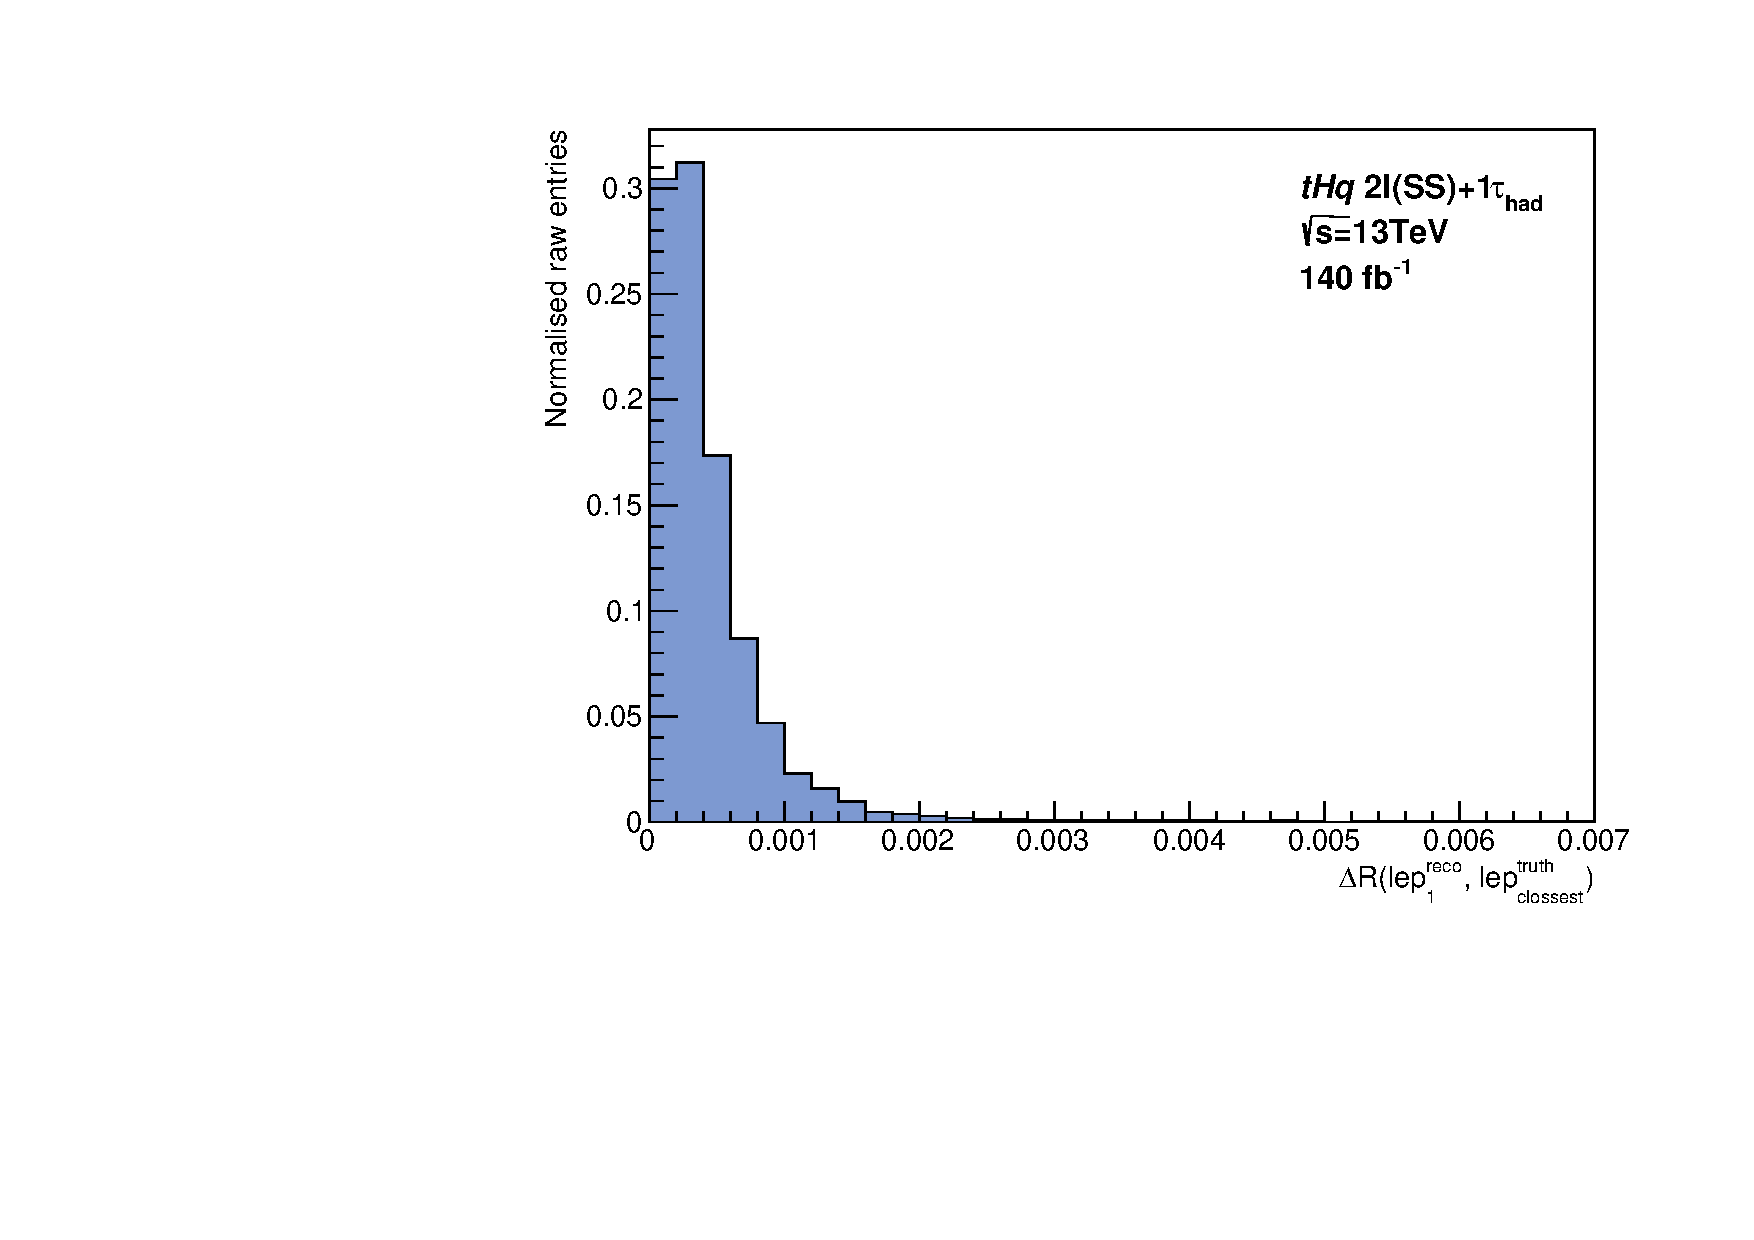
\includegraphics[width=\textwidth]{Chapter5_tHq/LeptAssociation/DeltaR_Cones/SS_only_TruthTopWLep_better_Lep_1_Zoom_1}
        \caption{$\Delta R(\ell_{1}^{\text{reco}}, \ell_{\text{closest}}^{\text{truth}})$}
    \end{subfigure}
    \hfill % Fills the space between the subfigures
    \begin{subfigure}[b]{0.495\textwidth}
        \centering
        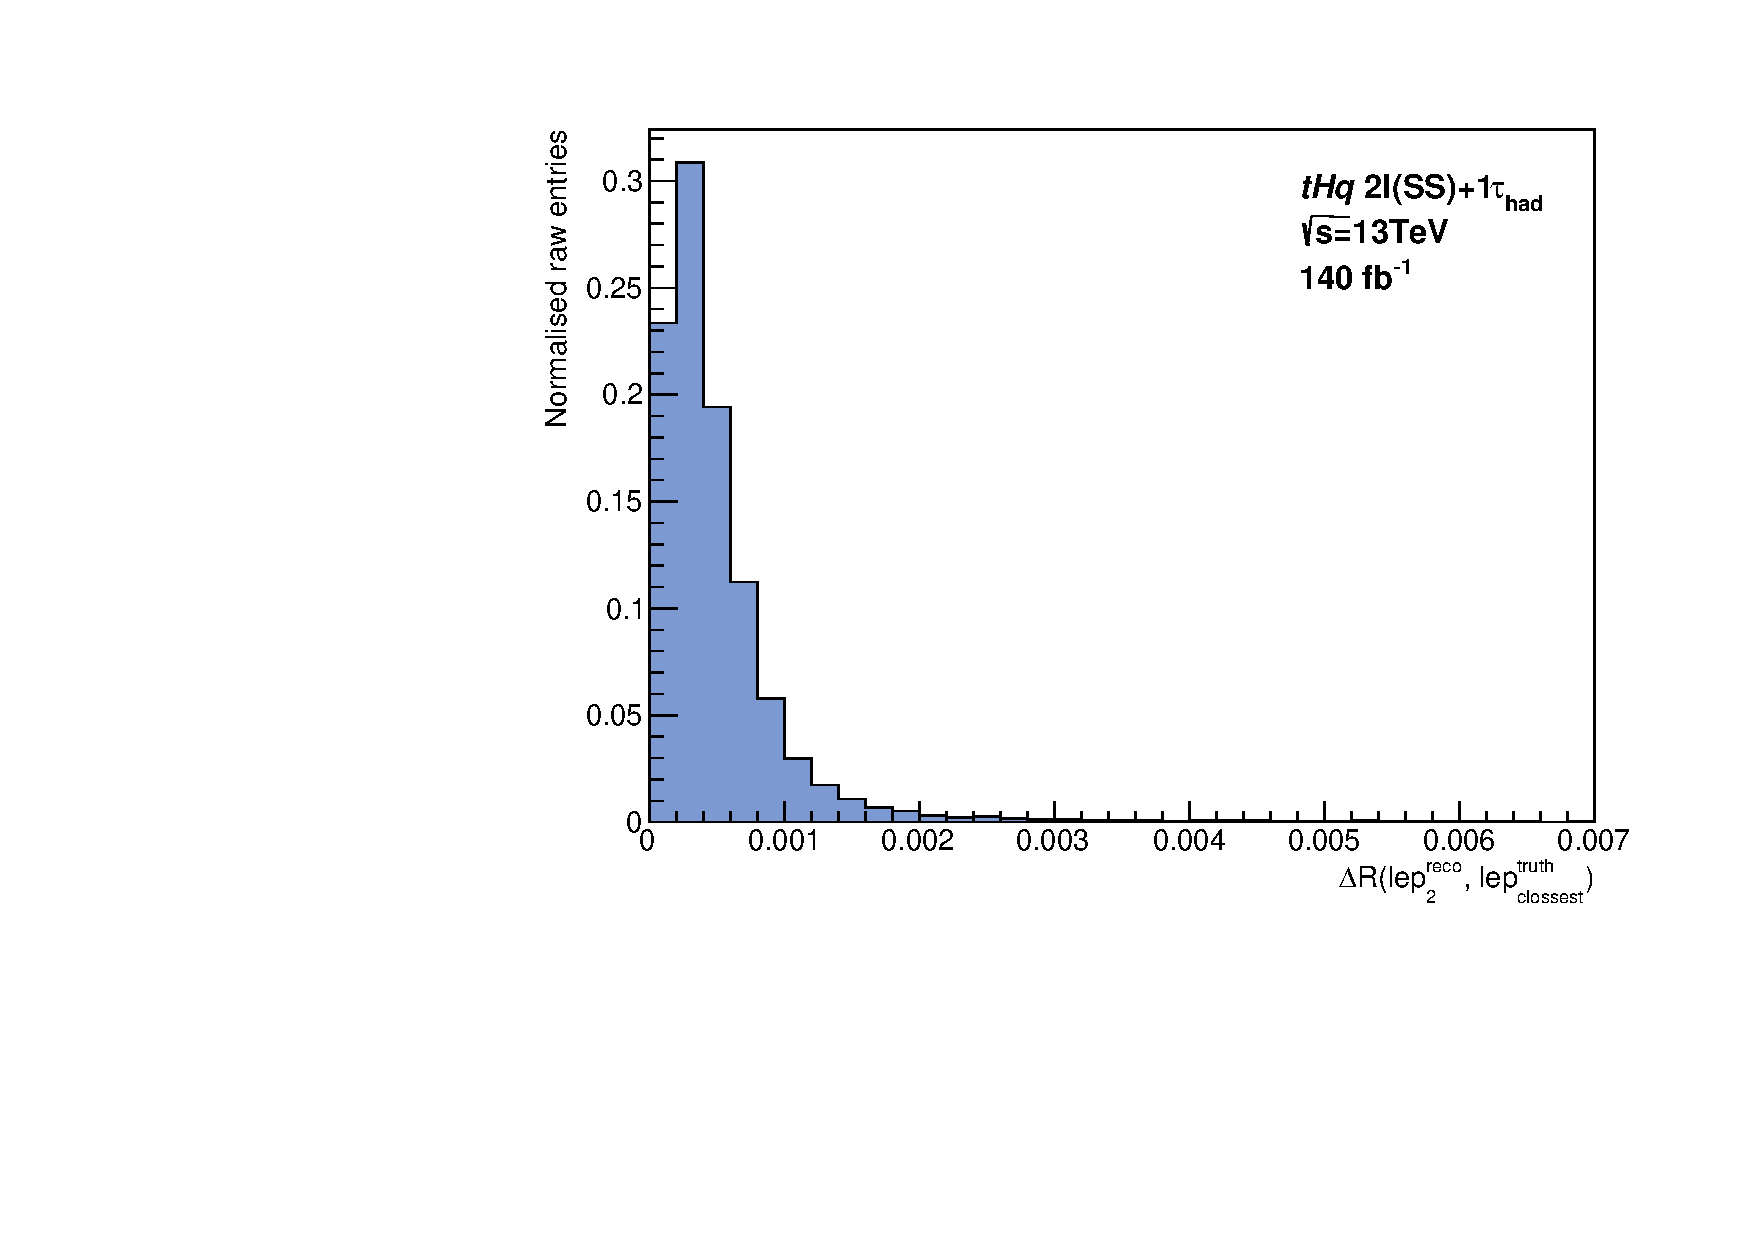
\includegraphics[width=\textwidth]{Chapter5_tHq/LeptAssociation/DeltaR_Cones/SS_only_TruthTopWLep_better_Lep_2_Zoom_1}
        \caption{$\Delta R(\ell_{2}^{\text{reco}}, \ell_{\text{closest}}^{\text{truth}})$}
    \end{subfigure}   
    \caption{Normalised distribution of the $\Delta R$ distance between the reconstructed light leptons and the 
    closest parton-level lepton in the \dilepSStau channel. The events are unweighted. 
    Note how, by demanding $\dR < 0.01$,    the leptons find a match in the majority of situations.}
    \label{fig:chap:tH:LepAssign:DeltaR}
\end{figure}



\begin{figure}[h]
\centering
\begin{subfigure}{.49\textwidth}
  \centering
  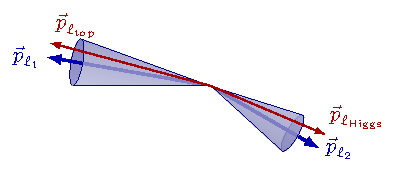
\includegraphics[width=\linewidth]{Chapter5_tHq/LeptAssociation/LepAssignement_2Matches_Type1}
  \caption{Two matches. Type$\,$1 event}
  \label{fig:chap:tH:LepAssign:Match:Type1}
\end{subfigure} 
\begin{subfigure}{.49\textwidth}
  \centering
  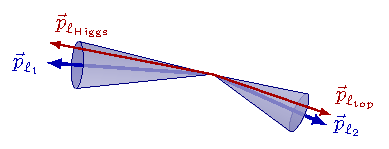
\includegraphics[width=\linewidth]{Chapter5_tHq/LeptAssociation/LepAssignement_2Matches_Type2}
  \caption{Two matches. Type$\,$2 event}
  \label{fig:chap:tH:LepAssign:Match:Type2}
\end{subfigure}

\begin{subfigure}{.49\textwidth}
  \centering
  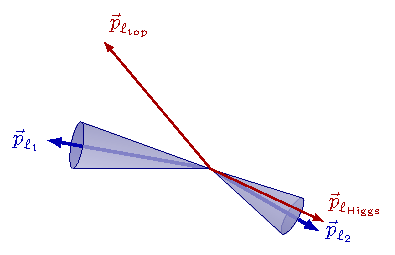
\includegraphics[width=\linewidth]{Chapter5_tHq/LeptAssociation/LepAssignement_1Match_Higgs_subleading}
  \caption{One match.}
  \label{fig:chap:tH:LepAssign:Match:1Match}
\end{subfigure}\hfill
\begin{subfigure}{.49\textwidth}
  \centering
  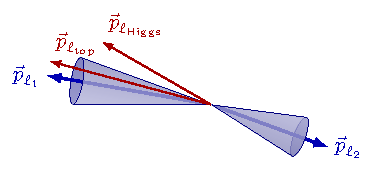
\includegraphics[width=\linewidth]{Chapter5_tHq/LeptAssociation/LepAssignement_1Match_Higgs_leading_b}
  \caption{One match.}
  \label{fig:chap:tH:LepAssign:Match:1Match_b}
\end{subfigure}

\begin{subfigure}{.5\textwidth}
  \centering
  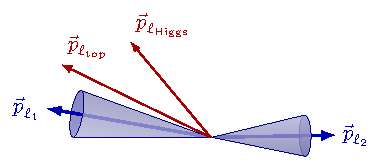
\includegraphics[width=.99\linewidth]{Chapter5_tHq/LeptAssociation/LepAssignement_0Matches_b}
  \caption{No matches}
  \label{fig:chap:tH:LepAssign:Match:0Matchs}
\end{subfigure}
\caption{	Different scenarios for the association between reconstruction-level (blue arrow) 
		and parton-level (red arrow ) light leptons. 
		Note that the labels $\Pl_{\text{top}}$ and $\Pl_{\text{Higgs}}$ are only available 
		for the parton-level particles. The labelling of the events is performed only for the 
		cases in (a) and (b).}% and saved in the variable \texttt{isLep1fromTop}.}
\label{fig:chap:tH:LepAssign:Match}
\end{figure}
%For this draw the https://tikz.net/jet_top/ package on latex has been used

To perform this labelling, it has been required that the \tauhad is originated in from the Higgs-boson 
system. This is imposed in order to guarantee that there are both a $\Pl_{\text{top}}$ and a $\Pl_{\text{Higgs}}$. 
This condition is satisfied to more than 80\% of events.
The Higgs-boson decay channels used for these studies are the \Htautau (one $\Ptau$ decaying leptonically 
and the other hadronically) and the \HWW. The \HZZ channel has not been included since its impact 
in the on the \dileptau production when the \tauhad comes from the Higgs boson is negligible. If the \tauhad is
originated in the Higgs-boson system, only 2.0\% of the events correspond to the \HZZ decay channel, 
in contrast to the 76.5\% of the \Htautau and the 21.5\% of the \HWW. These numbers are
presented in Table~\ref{tab:chap:tH:LepAssign:FractionInSS}. Once all these conditions have bee
applied,  a minimum distance between
each of the reconstructed leptons to its correspondent parton-level lepton, $\Delta R^{\ell_{1}, \ell_{2}}_{min}$ 
is demanded. The corresponding entry counts at each step are summarised in
Table~\ref{tab:chap:tH:LepAssign:LabellingFrac}. Note that the numbers are not the event yields 
but the entries, i.e, counting the raw number of MC events with no weights into consideration.
More information about event weights is given in 
Appendix~\ref{chap:Appendix:NegWeights}.

\begin{table}[h]
\centering
\begin{tabular}{l|l}
\toprule
Channel 	& Fraction (\%)   \\ \midrule
\Htautau 	& 76.52 \\
\HWW     	& 21.52 \\
\HZZ   	& 1.956 \\ \bottomrule
\end{tabular}
\caption{Contribution of each Higgs-boson decay channel to the \dileptau final state when
demanding that the \tauhad is originated from the Higgs-boson decay chain.
The numbers in this table are calculated from the rightmost column 
of Table~\ref{tab:ChaptH:TruthSummary}.}
\label{tab:chap:tH:LepAssign:FractionInSS}
\end{table}


%Following the application of criteria related to the multiplicity of \bjets, electrons, and muons, 
%as well as the requirement that the Higgs boson decays to \Htautau or \HWW, the matching 
%condition is imposed to set the label.
% This condition demands a minimum distance between
%each of the reconstructed leptons to its correspondent parton-level lepton, $\Delta R^{\ell_{1}, \ell_{2}}_{min}$.
%As each condition is sequentially applied, a reduced number of events satisfy the imposed filters. 
%The corresponding entry counts at each step are summarised in
%Table~\ref{tab:chap:tH:LepAssign:LabellingFrac}. Note that the numbers are not the event yields 
%but the entries, i.e, counting the raw number of MC events with no weights in consideration.
%More information about event weights is given in 
%Appendix~\ref{chap:Appendix:NegWeights}.

\begin{table}[h]
\centering
\begin{tabular}{l|l}
\toprule
Stage								&  Entries \\ \midrule
Total \tHq (\dileptau) sample                               & 43922 \\
%Preselection: $2\emu$, $1 \Ptau$, at least $1 \bjet$ & 30113 \\
\dilepSStau sample						& 18140 \\
Selection:  $\PHiggs \rightarrow \taulep\tauhad/\PWplus\PWminus$ , $\PW \rightarrow \Pe / \Pmu / \taulep$ & 15446 \\
$\Delta R(\ell_{1}^{\text{reco}}, \ell_{\text{closest}}^{\text{truth}}) < 0.01$ and $\Delta R(\ell_{2}^{\text{reco}}, \ell_{\text{closest}}^{\text{truth}}) < 0.01$
                                						& 14680 \\ \bottomrule
\end{tabular}
\caption{Unweighted (raw) events at each step of the labelling 
process. 
%Unweighted means that, when counting the 
%events, each entry is taken as one rather than taking into account the event 
%weight. More information about event weights is given in 
%Appendix~\ref{chap:Appendix:NegWeights}.
The first row corresponds to the entire sample of just \tHq events in the \dileptau channel after the preselection requirements (see Section~\ref{sec:ChaptH:EventSelection:PR}). 
The second row applies the condition on the charge of the light leptons.
The third refers to the subset of \dilepSStau events for which it is computed the $\Delta R$ distance between 
the truth- and reconstruction-level  leptons. The $\PW \rightarrow \Pe / \Pmu / \taulep$ condition enforces that
the \tauhad is produced in the Higgs-boson system. 
Finally, the last row demands that both leptons at reconstruction level have are matched to different truth-level leptons.}
% $\Delta R^{\ell_{1}, \ell_{2}}_{min}$ is
%within 0.01, where 
%$\Delta R^{\ell_{1}, \ell_{2}}_{min} = \text{min}\left(\Delta R(\protect\overrightarrow{p}_{\ell_{1}, \ell_{2}}, \protect\overrightarrow{p}_{\ell_{\text{Top}}}),\Delta %R(\protect\overrightarrow{p}_{\ell_{1}, \ell_{2}}, \protect\overrightarrow{p}_{\ell_{\text{Higgs}}}) \right)$. 
%} %Being $\protect\overrightarrow{p}_{\ell}$ the momentum of the lepton.
\label{tab:chap:tH:LepAssign:LabellingFrac}
\end{table}

%\pablo{Should add the fraction of events that are labelled from a) the total \dileptau sample and b) from the total \dilepSStau .}
 
 
%%%%%%%%%%%%%%%%%
%           Input variables     	 %
%%%%%%%%%%%%%%%%%
\subsubsection{BDT input features}
\label{sec:ChaptH:Sig:LepAsign:SS:BDT:inputFeatues}
The choice of input variables for training a BDT is a crucial factor for achieving good classification accuracy.
The chosen variables must exhibit the ability to effectively differentiate between Type$\,$1 and Type$\,$2. 
Nine variables have been used. Figure~\ref{fig:ChaptH:LepAsign:SS:BDT:inputFeatuerRanked} presents
the distributions of the highest ranked.
Appendix~\ref{chap:Appendix:BDT_Variables:LepAssignment} shows
the distributions of the other five. In these plots can be seen 
the Type$\,$1 and Type$\,$2 present different profiles for the same variable.
This divergence in shapes indicates the efficacy of these variables for classifying.

The TMVA package is capable of ranking variables within its model based on how often the 
variables are used to split decision tree nodes, and by weighting each split occurrence by 
the separation gain-squared\footnote{See Equation~\ref{eq:Appendix:BDT:SeparationPower} 
in Appendix~\ref{chap:Appendix:BDT} for more details.}
 ($<S^{2}>$) it has achieved and by the number of events in the node~\cite{Breiman1984ClassificationAR}.
The variables employed in the model, ordered according to their respective levels of importance, are as follows:
\begin{itemize}
   	\item $m^{\text{opt1}}_{\text{vis}}(H)$: Mass of the \tauhad and the 
		leading\footnote{Note that the term ``leading'' refers to the \pT-leading. This applies for all its uses in this thesis.} light-lepton. %m\_Hvis\_opt1
		 $<S^{2}> = 3.734 \times 10^{-1}$.
   	\item $\Delta \eta(\tauhad, \ell_{1})$: $\Delta \eta$ between the 
		\tauhad and the leading light-lepton. %deltaEta\_tau\_LightLep1
		 $<S^{2}> = 2.457 \times 10^{-1}$.
    	\item $m^{\text{opt2}}_{\text{vis}}(H)$: Mass of the combined \tauhad and 
		the sub-leading light-lepton. %m\_Hvis\_opt2
		 $<S^{2}> = 2.025 \times 10^{-1}$.
   	\item $\Delta \eta(\tauhad, \ell_{2})$: $\Delta \eta$ between the 
		\tauhad and the sub-leading light-lepton. %deltaEta\_tau\_LightLep2
		 $<S^{2}> = 1.864 \times 10^{-1}$.
    	\item $m^{\text{opt1}}_{\text{pred}}(t)$: Mass of the leading \btagged jet, the leading light-lepton, and the predicted energy for the corresponding neutrino.  %m\_Tpred\_opt1
		 $<S^{2}> = 1.596 \times 10^{-1}$.
    	\item $\Delta R(b\text{-tagged jet}, \ell_{1})$: $\Delta R$ between the leading
		$b$-tagged jet and the leading light-lepton. %deltaR\_b\_LightLep1
		 $<S^{2}> = 1.142 \times 10^{-1}$.
    	\item $m^{\text{opt2}}_{\text{pred}}(t)$: Mass of the leading \btagged jet, the sub-leading lepton and the predicted energy for the corresponding neutrino.
		of the $\ell_{2}$. %$m_{\text{pred}}(t) = \sqrt{(P_{b}+P_{\ell}+P_{\nu, pred})^}{2}$%m\_Tpred\_opt2
		 $<S^{2}> = 1.104 \times 10^{-1}$.
	\item $\Delta R(b\text{-tagged jet}, \ell_{2})$: $\Delta R$ between the  leading
		$b$-tagged jet and the sub-leading light-lepton.%deltaR\_b\_LightLep2
		 $<S^{2}> = 1.009 \times 10^{-1}$.
    	\item $\Delta \eta(\text{closest }b\text{-tagged jet}, \text{leading lepton})$: 
		$\Delta \eta$ between the leading lepton and the closest \btagged 
		jet to that lepton.%¿?This lepton can either be a light lepton or the hadronic tau.
		%DeltaEtaLeadingLeptonClosestBjet			
		 $<S^{2}> = 7.401 \times 10^{-2}$.
\end{itemize}
The separation-power-based ranking of the $\text{BDT}^{\text{Lepton Assignment}}$ 
input variables is derived by counting how often the variables are used to 
split decision tree nodes. Then, each split occurrence is weighted by the separation-gain squared 
it has achieved and by the number of events in the node~\cite{Breiman1984ClassificationAR}.
% source: 8.13.4 https://root.cern.ch/download/doc/tmva/TMVAUsersGuide.pdf
% source references: L. Breiman, J. Friedman, R. Olshen and C. Stone, “Classification and Regression Trees”, Wadsworth (1984).



\begin{figure}[h]
    \centering
    % First row
    \begin{subfigure}[b]{0.42\textwidth}
        \centering
        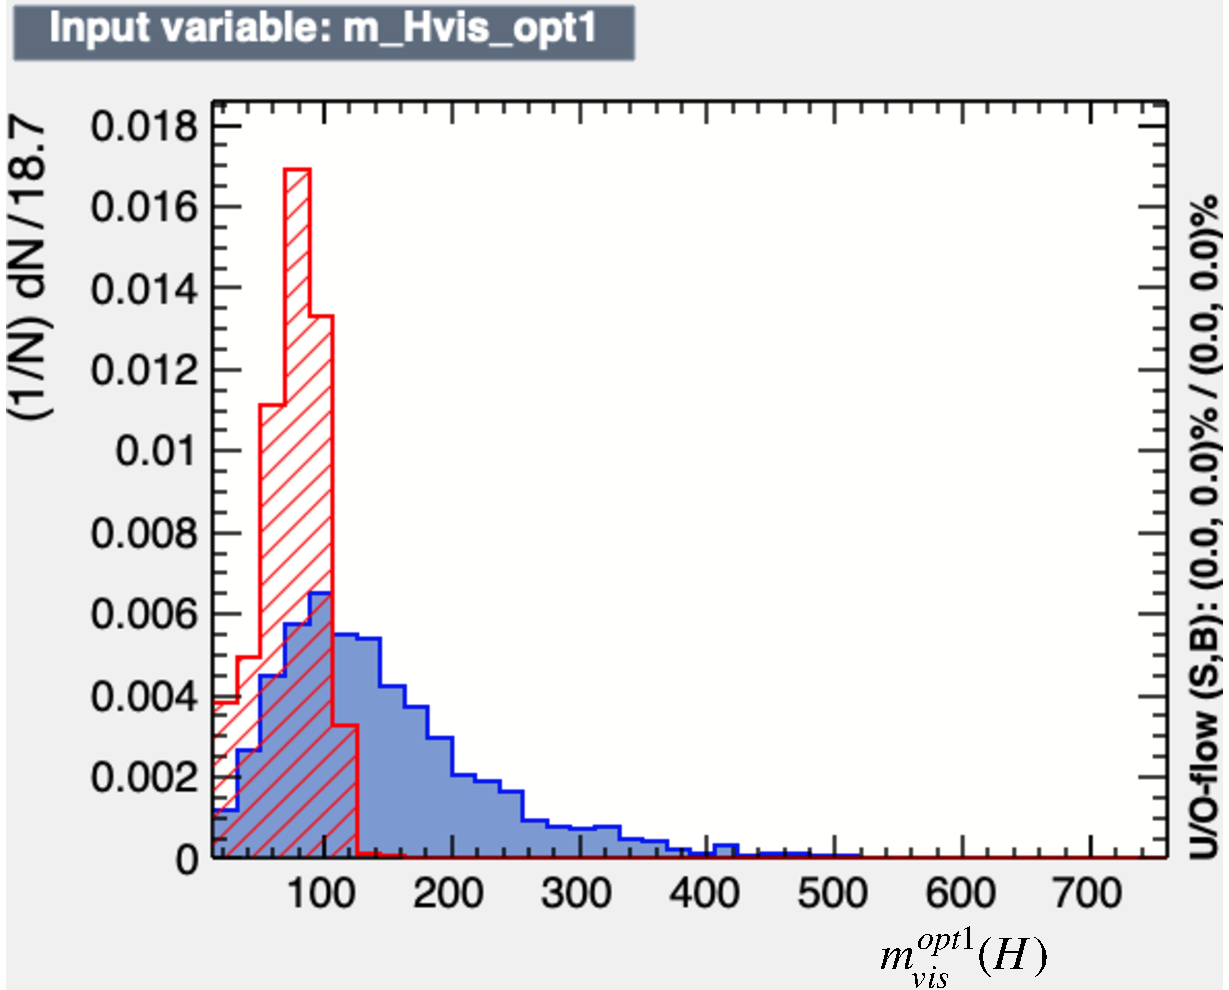
\includegraphics[width=\textwidth]{Chapter5_tHq/LeptAssociation/BDT_InputVariables/pdf_input_m_Hvis_opt1}
        \caption{$m^{\text{opt1}}_{\text{vis}}(H)$}
        \label{fig:ChaptH:LepAsign:SS:BDT:inputFeatuerRanked:m_H1}
    \end{subfigure}
    \hfill 
    \begin{subfigure}[b]{0.42\textwidth}
        \centering
        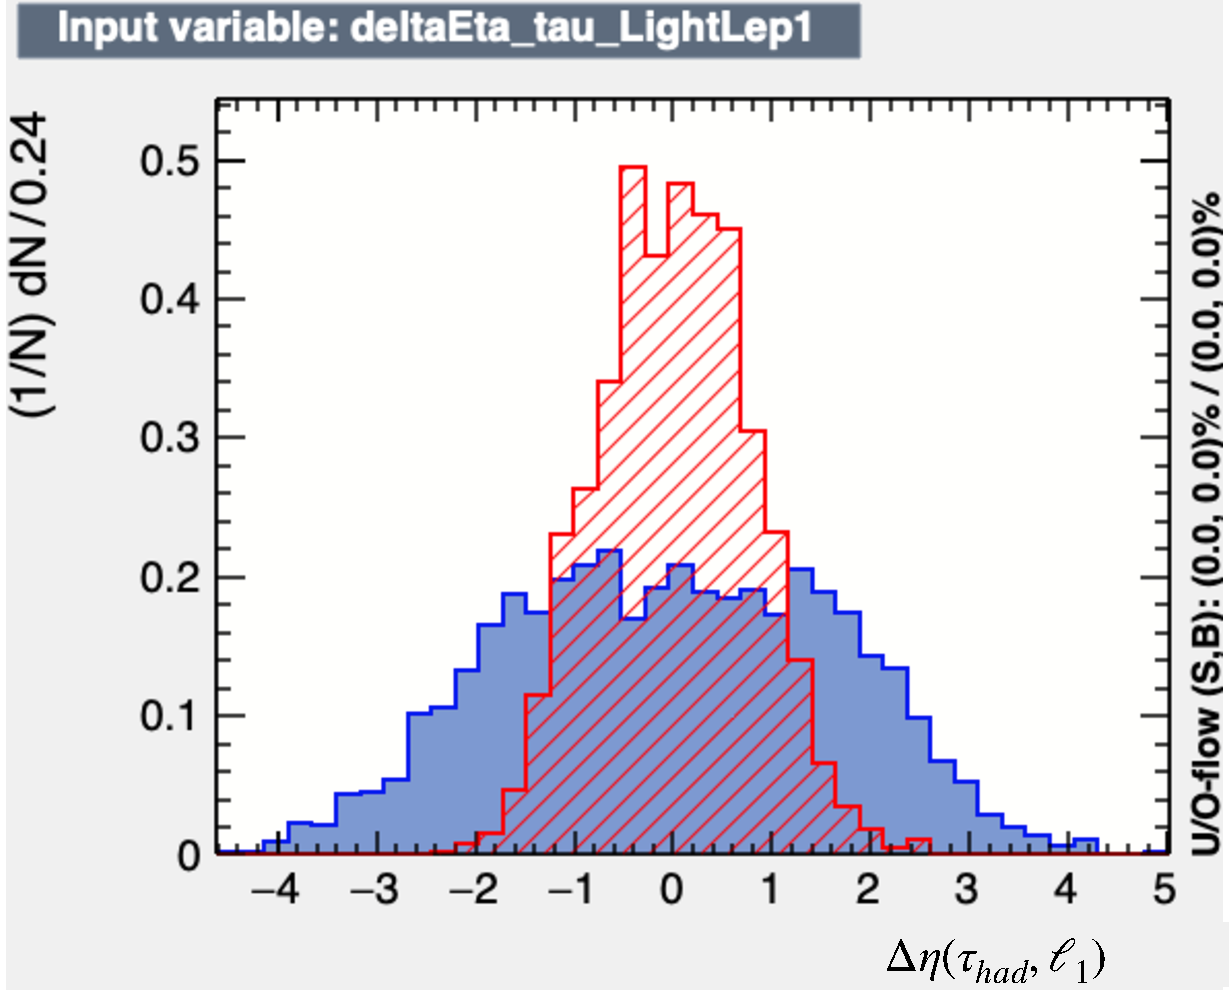
\includegraphics[width=\textwidth]{Chapter5_tHq/LeptAssociation/BDT_InputVariables/pdf_input_deltaEta_tau_LightLep1}
        \caption{$\Delta \eta(\tauhad, \ell_{1})$}
        \label{fig:ChaptH:LepAsign:SS:BDT:inputFeatuerRanked:dEta1}
    \end{subfigure}
    
    % Second row
    \begin{subfigure}[b]{0.42\textwidth}
        \centering
        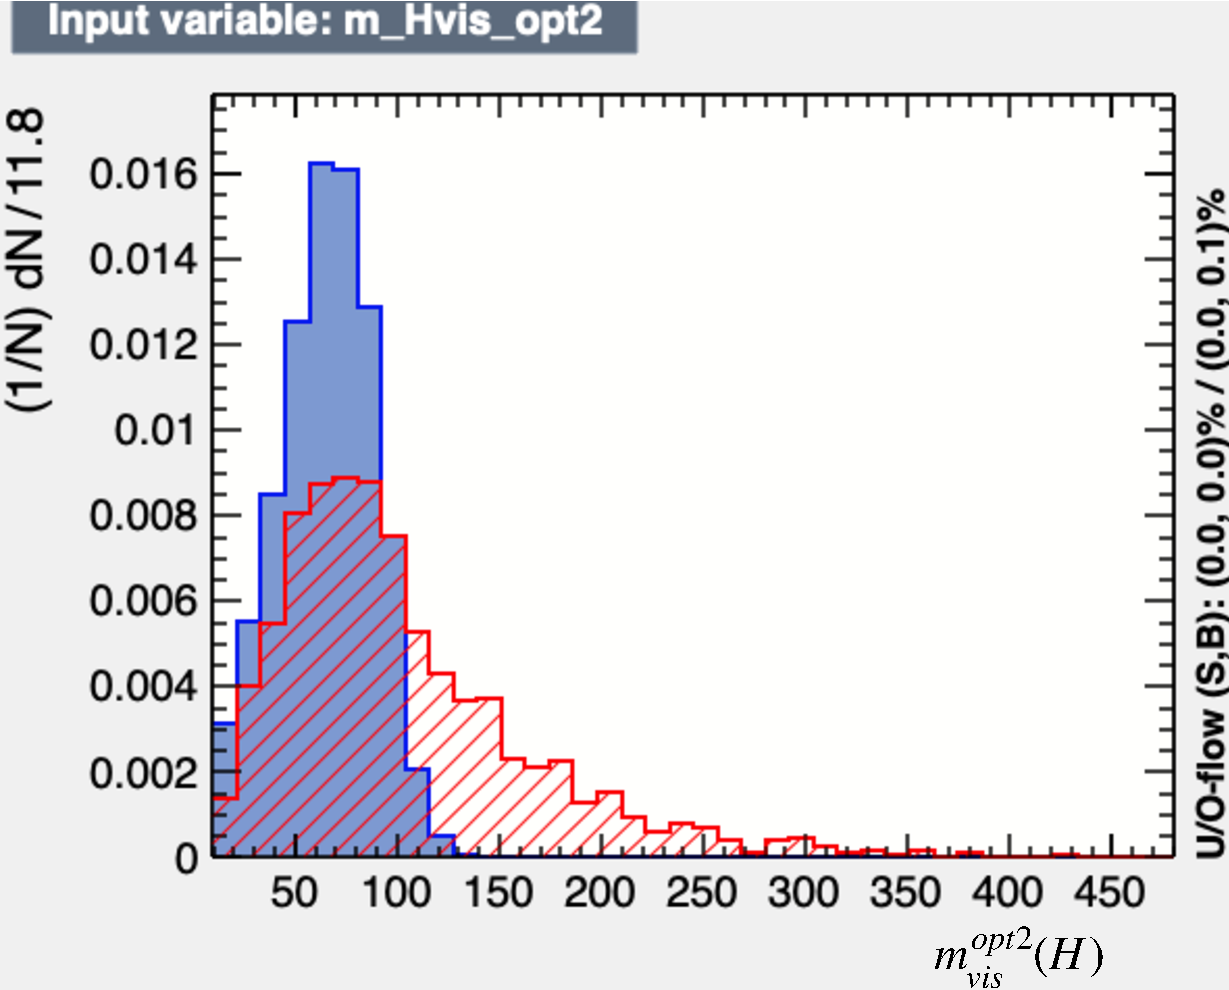
\includegraphics[width=\textwidth]{Chapter5_tHq/LeptAssociation/BDT_InputVariables/pdf_input_m_Hvis_opt2}
        \caption{$m^{\text{opt2}}_{\text{vis}}(\PHiggs)$}
        \label{ffig:ChaptH:LepAsign:SS:BDT:inputFeatuerRanked:m_H2}
    \end{subfigure}
    \hfill
    \begin{subfigure}[b]{0.42\textwidth}
        \centering
        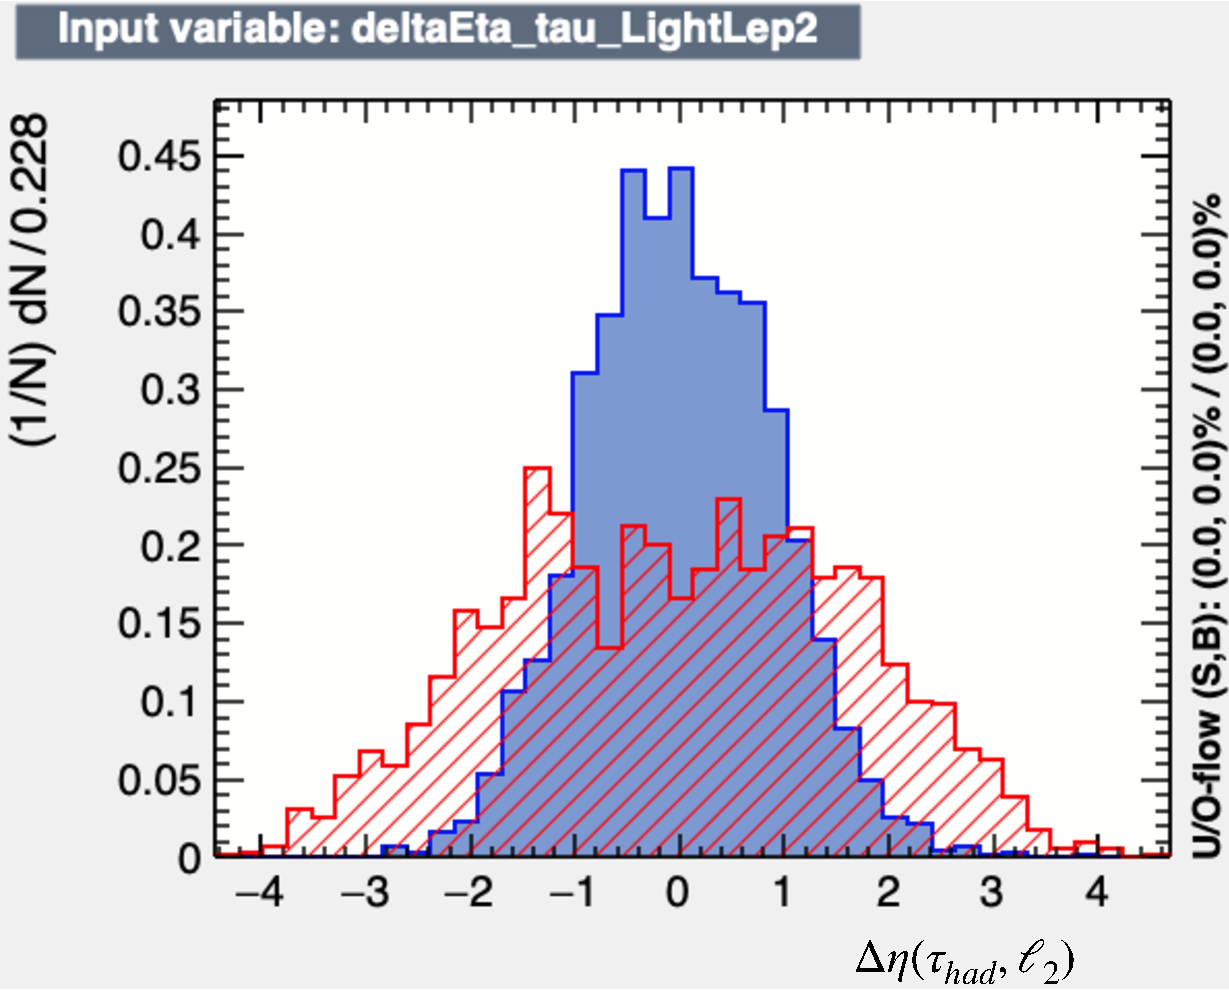
\includegraphics[width=\textwidth]{Chapter5_tHq/LeptAssociation/BDT_InputVariables/pdf_input_deltaEta_tau_LightLep2}
        \caption{$\Delta \eta(\tauhad, \ell_{2})$}
        \label{fig:ChaptH:LepAsign:SS:BDT:inputFeatuerRanked:dEta2}
    \end{subfigure}
    \caption{Normalised distributions of the highest ranked variables for the light-lepton assignment.}
    \label{fig:ChaptH:LepAsign:SS:BDT:inputFeatuerRanked}
\end{figure}



%\begin{figure}[h]
%\centering
%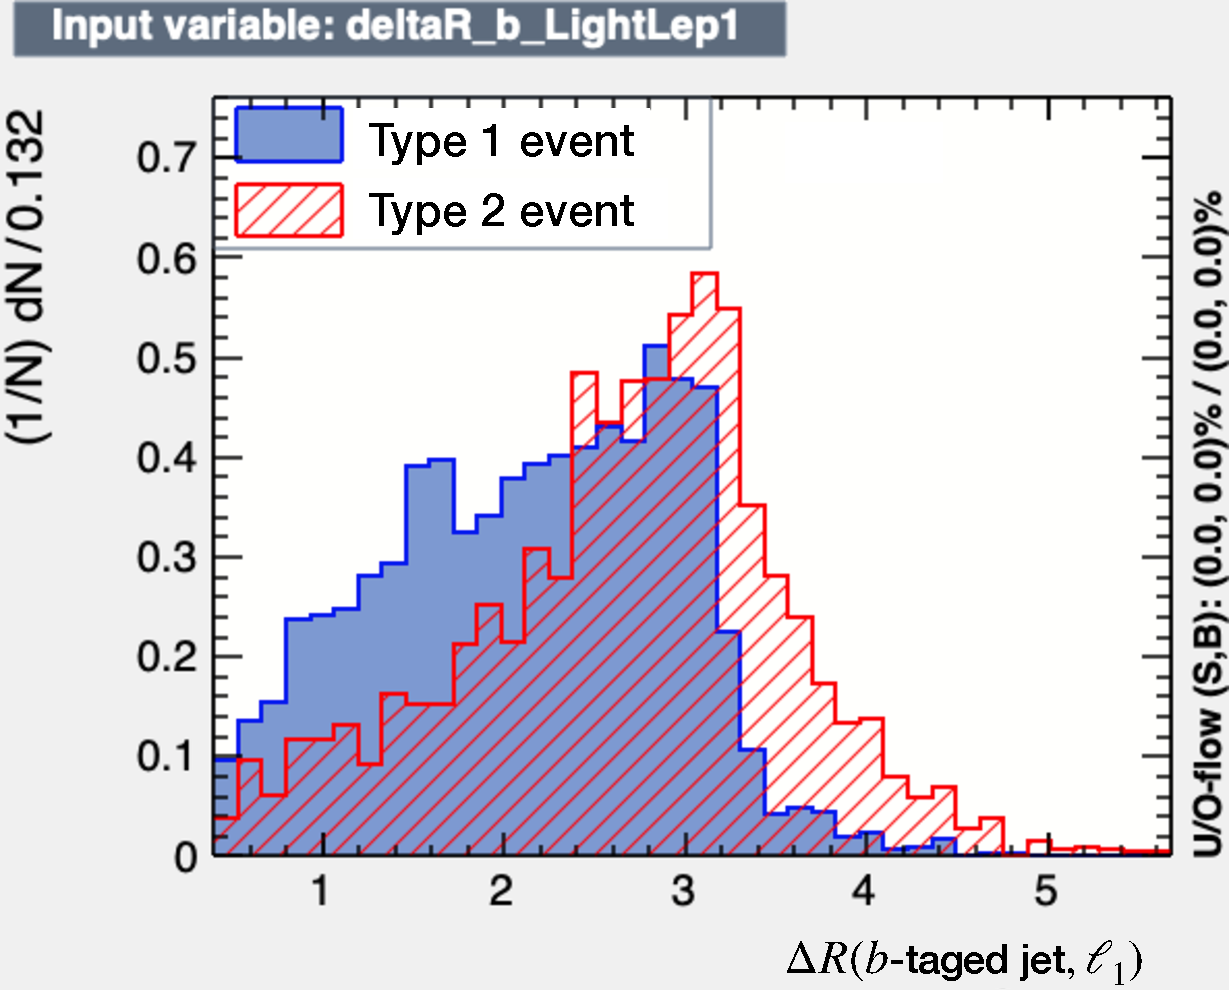
\includegraphics[width=.31\textwidth]{Chapter5_tHq/LeptAssociation/BDT_InputVariables/pdf_input_deltaR_b_LightLep1}\quad
%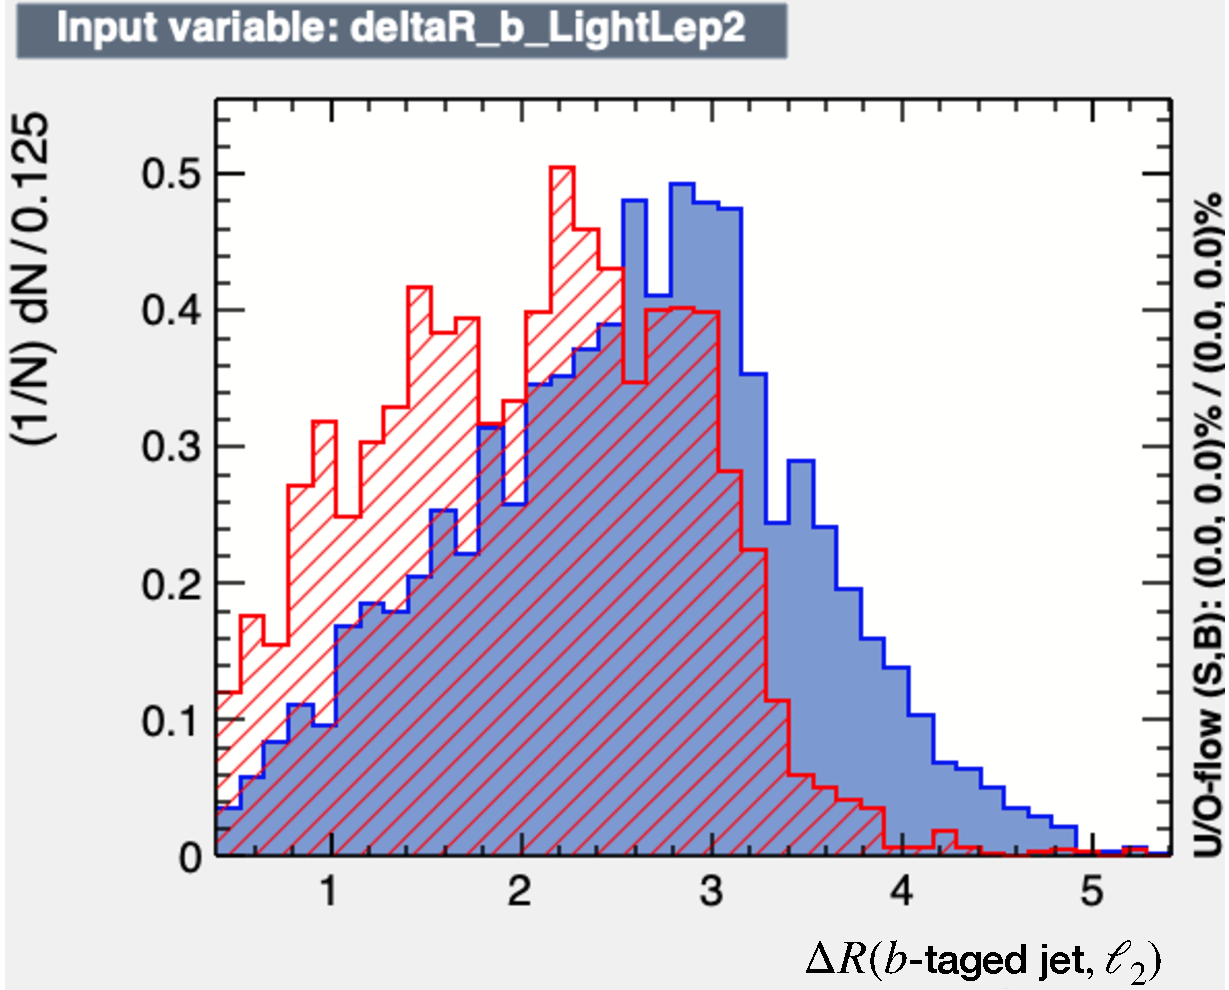
\includegraphics[width=.31\textwidth]{Chapter5_tHq/LeptAssociation/BDT_InputVariables/pdf_input_deltaR_b_LightLep2}\quad
%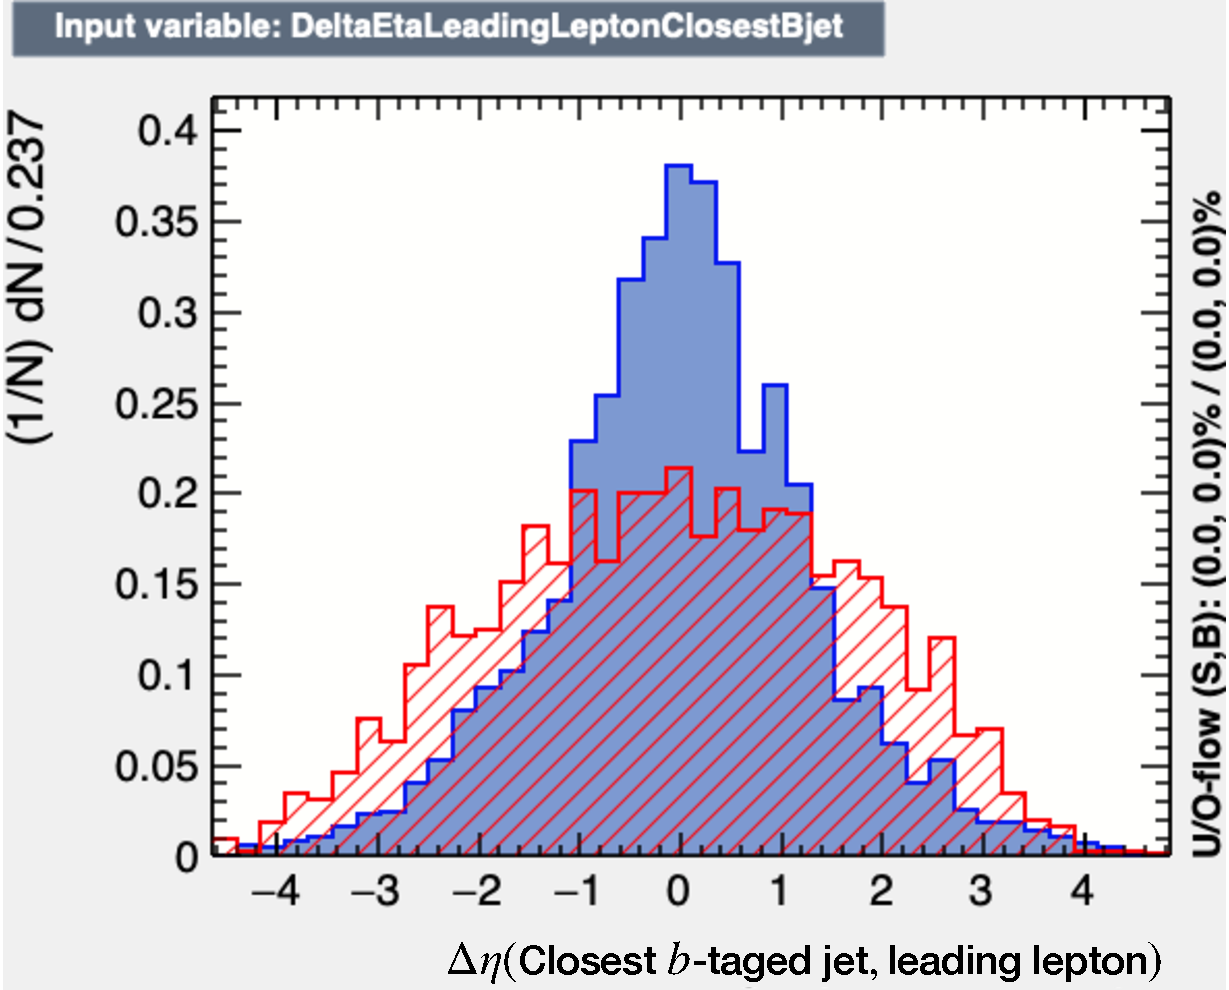
\includegraphics[width=.31\textwidth]{Chapter5_tHq/LeptAssociation/BDT_InputVariables/pdf_input_DeltaEtaLeadingLeptonClosestBjet}
%\medskip
%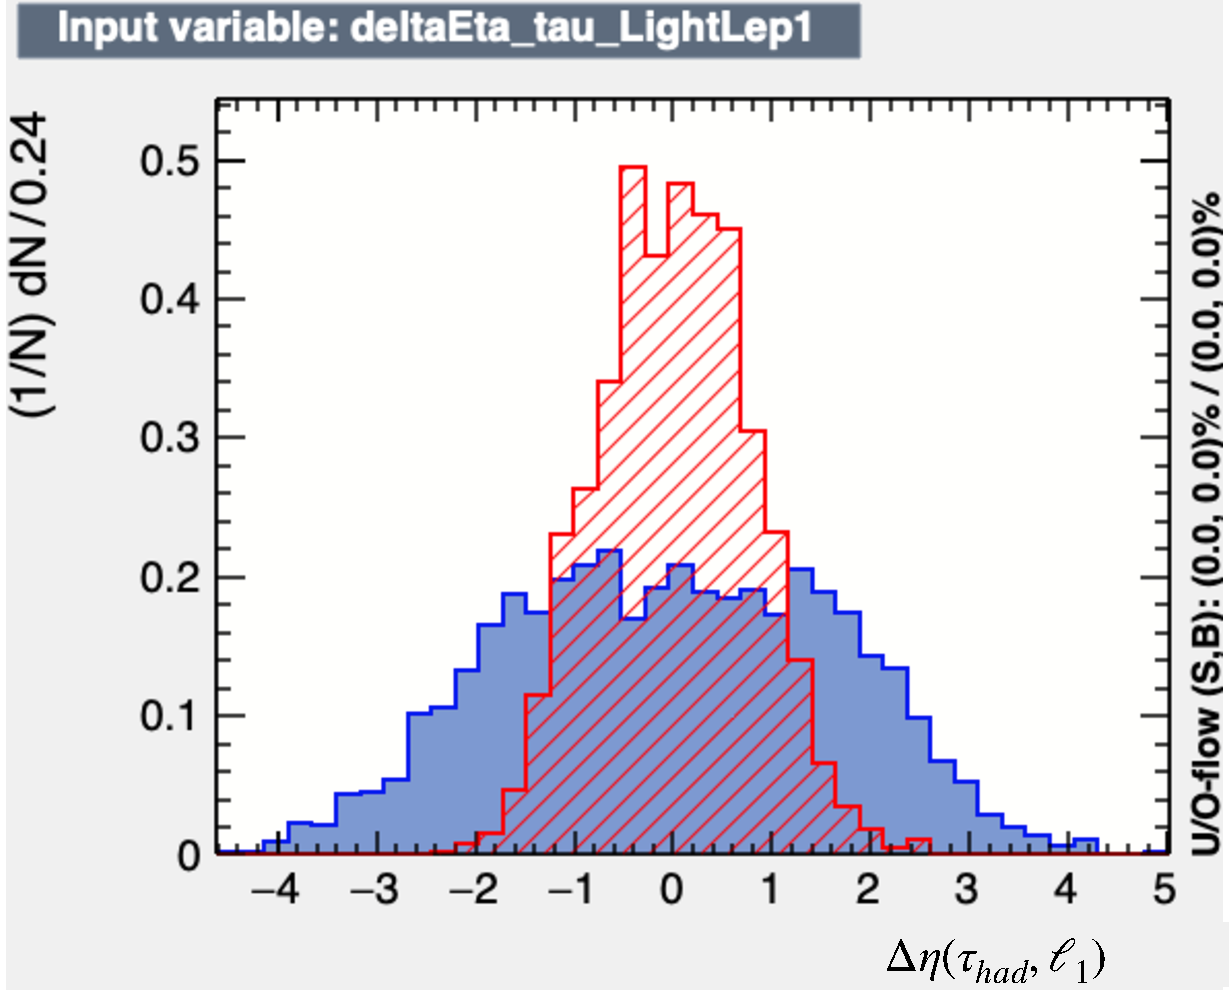
\includegraphics[width=.31\textwidth]{Chapter5_tHq/LeptAssociation/BDT_InputVariables/pdf_input_deltaEta_tau_LightLep1}\quad
%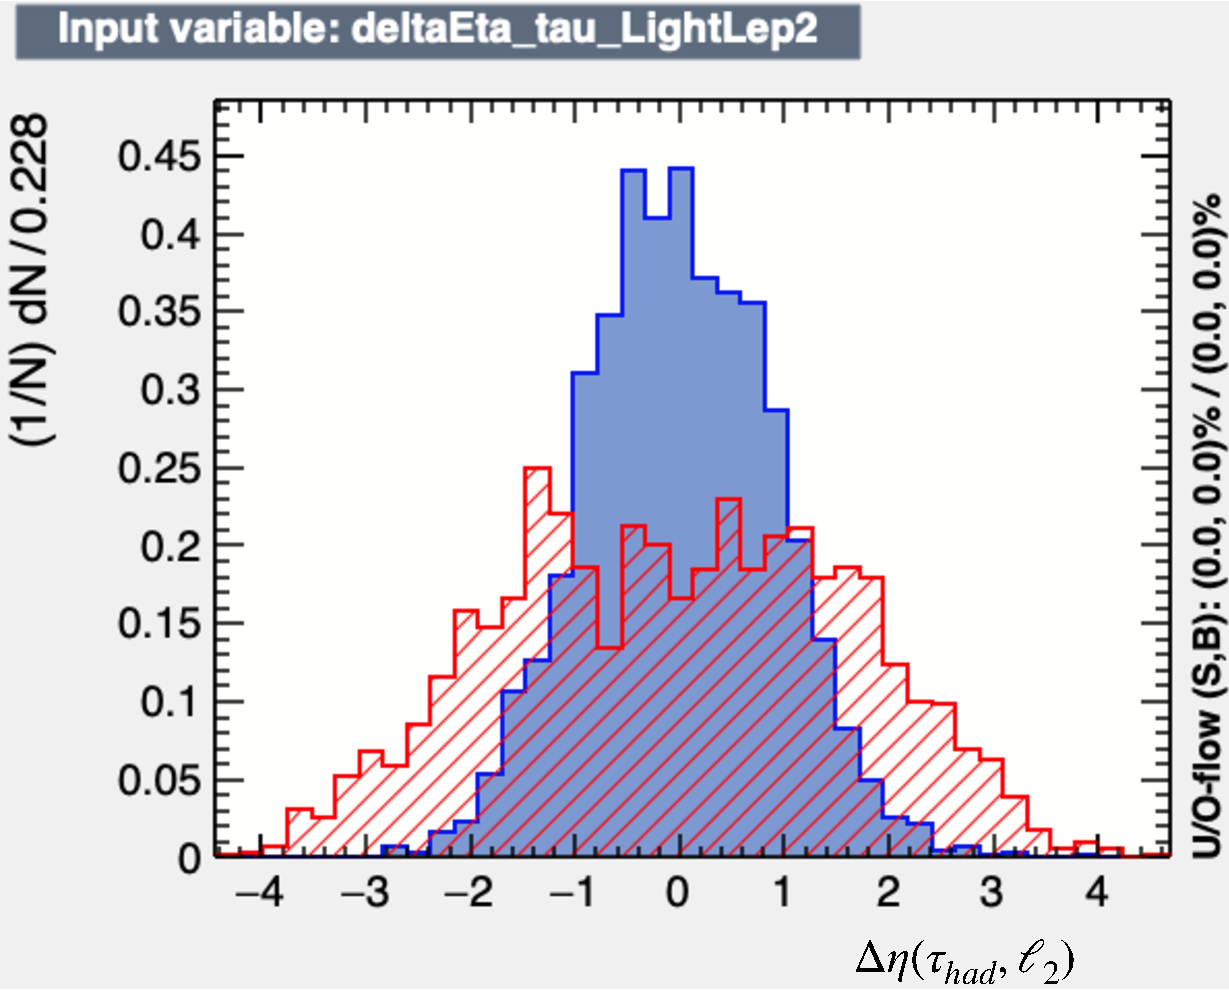
\includegraphics[width=.31\textwidth]{Chapter5_tHq/LeptAssociation/BDT_InputVariables/pdf_input_deltaEta_tau_LightLep2}\quad
%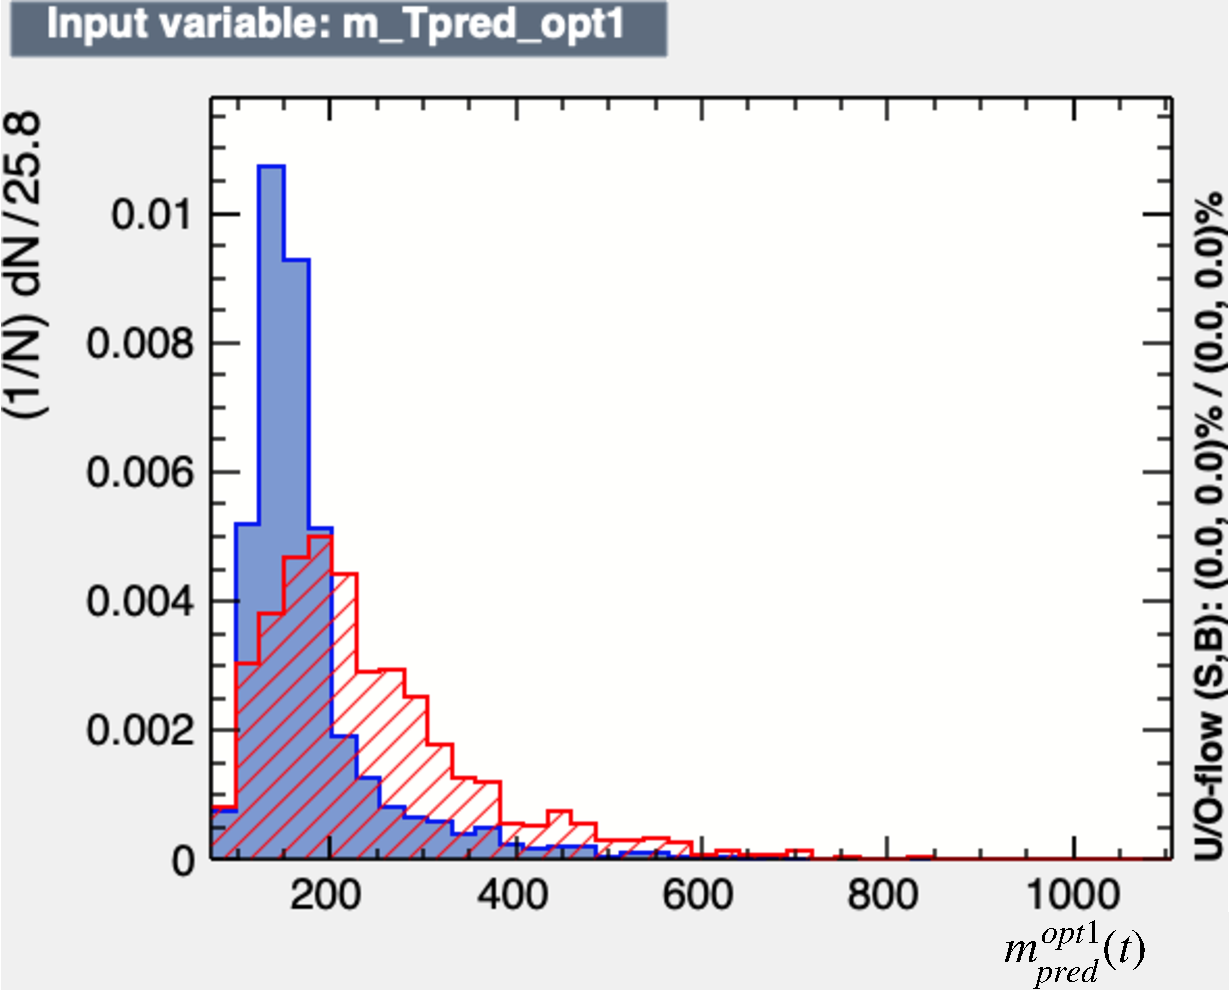
\includegraphics[width=.31\textwidth]{Chapter5_tHq/LeptAssociation/BDT_InputVariables/pdf_input_m_Tpred_opt1}
%\medskip
%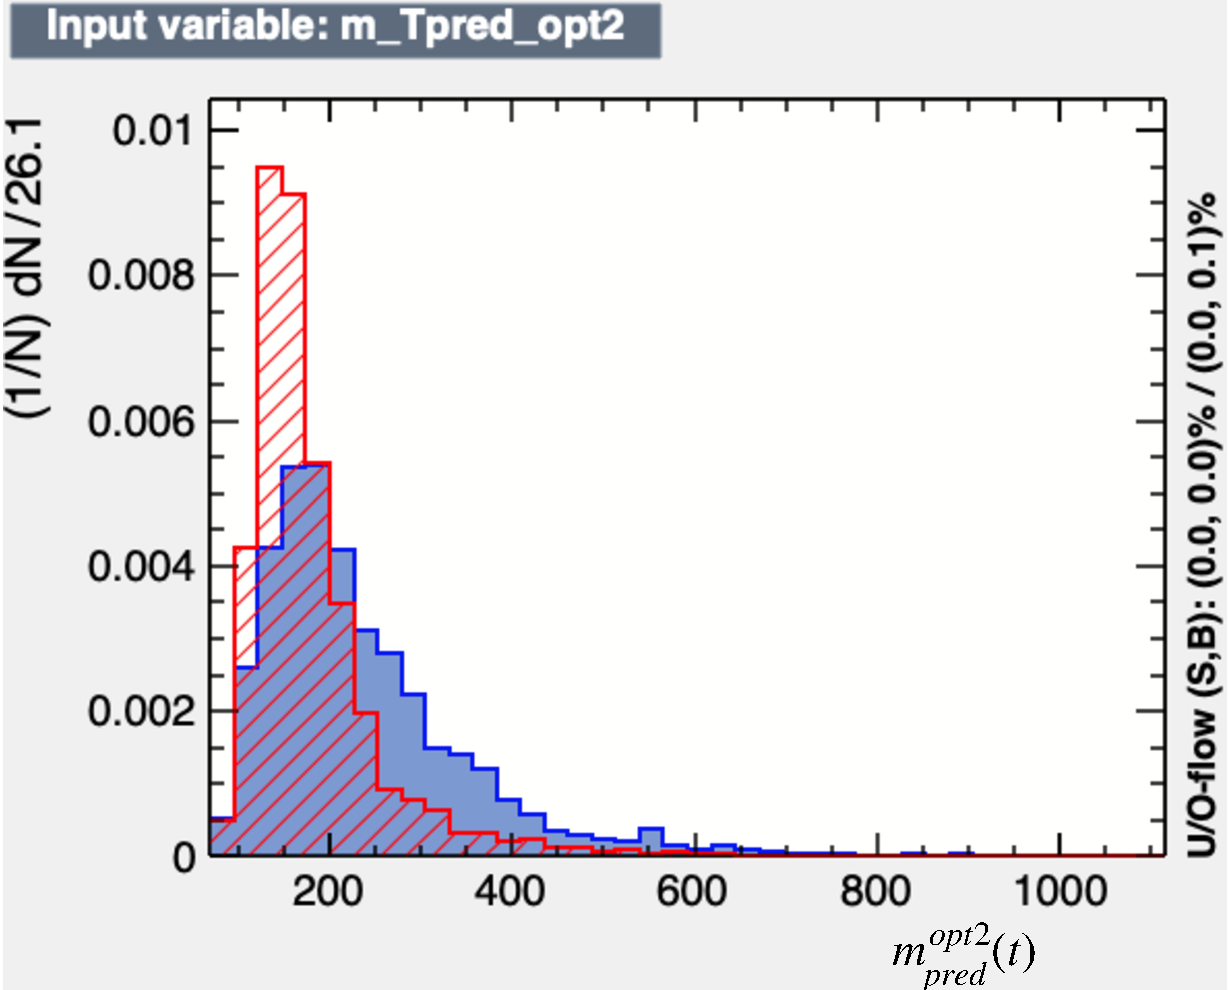
\includegraphics[width=.31\textwidth]{Chapter5_tHq/LeptAssociation/BDT_InputVariables/pdf_input_m_Tpred_opt2}\quad
%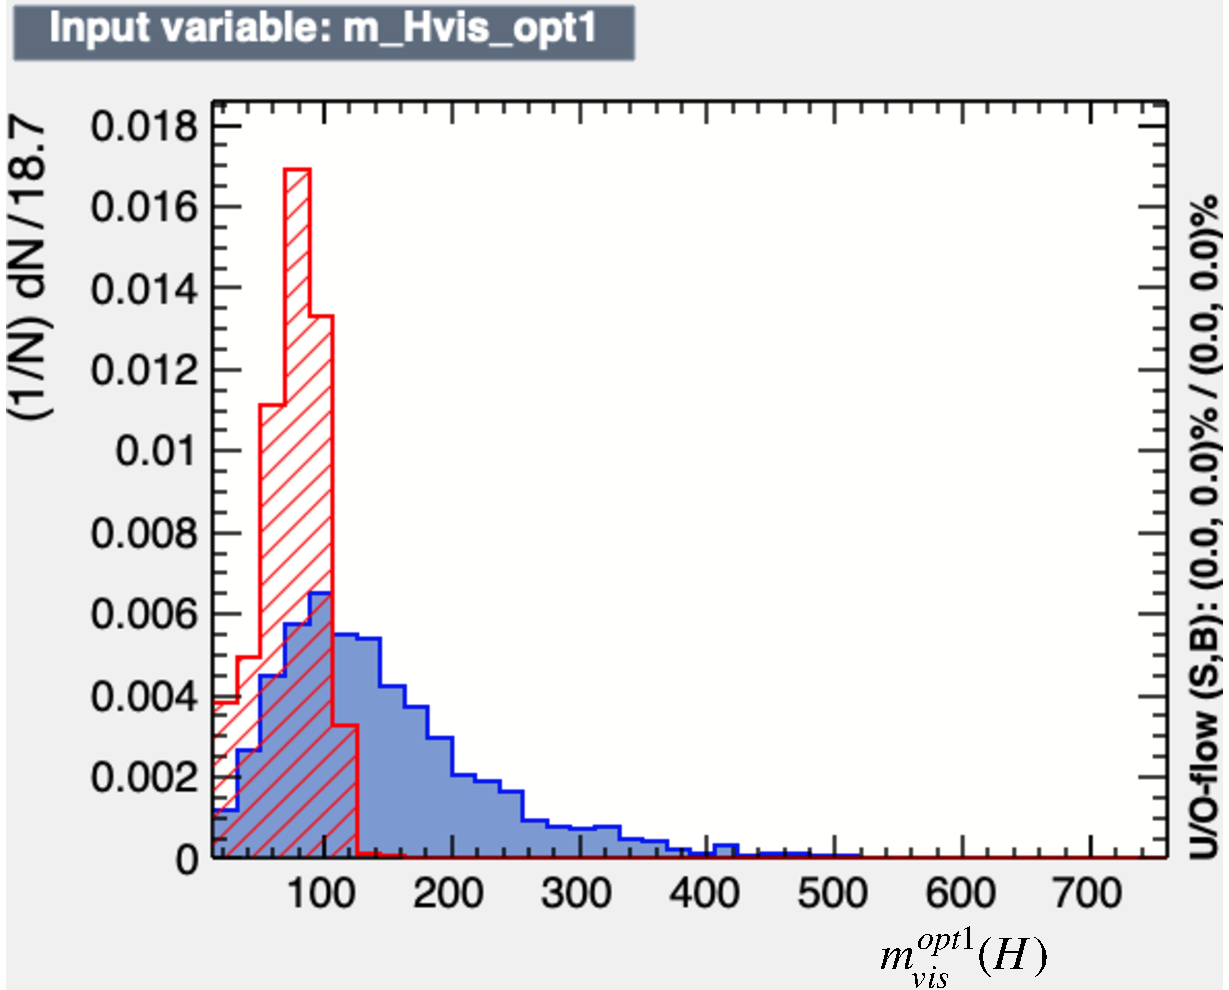
\includegraphics[width=.31\textwidth]{Chapter5_tHq/LeptAssociation/BDT_InputVariables/pdf_input_m_Hvis_opt1}\quad
%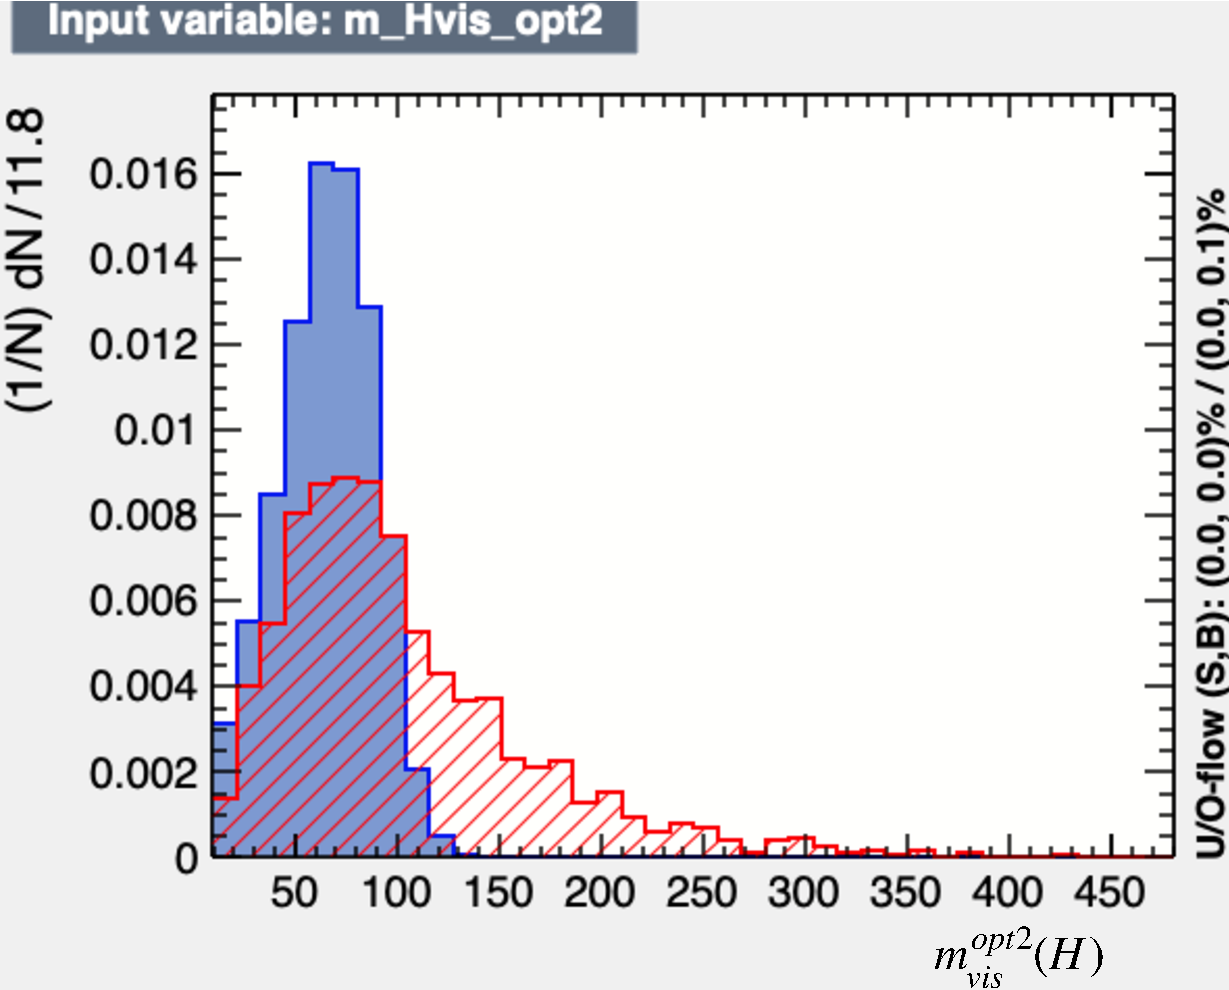
\includegraphics[width=.31\textwidth]{Chapter5_tHq/LeptAssociation/BDT_InputVariables/pdf_input_m_Hvis_opt2}
%\caption{Input variables for the $\text{BDT}^{\text{Lepton Assignment}}$. 
%In blue the events in which the $\ell_{1}$ comes from the top quark decay
%and in red those for which $\ell_{1}$ is produced from the Higgs boson. 
%Note that only events that contain the truth-reco matching described 
%in Section~\ref{sec:tHq:origin:LeptonAssignment_truth_reco_DeltaRCone} are used to produce these plots.}
%\label{fig:dileptau:Assignment_appendix:InputVars}
%\end{figure}

Furthermore, it is important that the selected variables are not highly correlated, as correlations 
can exacerbate model complexity and result in redundant information that provides no improvement to model performance.
% Keep in mind that more complex models can be harmful since the computational times to operate the model increase and
% High correlations can lead to overfitting, where the model becomes too complex and 
% performs well on the training set but poorly on new, unseen data.
Figure~\ref{fig:dileptau:Assignment_appendix:InputVars:Correlations} present the 
correlation matrices for the final input variables. A correlation matrix is a square 
matrix that provides a comprehensive view of the correlation coefficients between 
multiple variables. Note that these matrices show the bidimensional linear correlation coefficients
but the BDT uses N-dimensional relations so relevant higher-order relations cannot be
uncovered by the matrices.

When using larger sets of input features, as expected, an increase in the number 
of highly correlated pairs of variables is observed. To address this concern, for each 
correlated variable pair, the variable with lower separation power is removed from the model.
The separation power ranking is automatically built during the training.

%Note that in Figure~\ref{fig:dileptau:Assignment_appendix:InputVars:Correlations} 
%there are still some pairs of collinear variables such as $m^{\text{opt2}}_{\text{pred}}(t)$ and 
%$\Delta R(b\text{-tagged jet}, \ell_{2})$. One could think that one of these two should 
%be eliminated from the model but since the correlation is only present in one 
%category (Type$\,$1 in this case) it can still be used because it provides identification
%power in the other.

\begin{figure}[h]
\centering
\begin{subfigure}[b]{0.8\textwidth}
   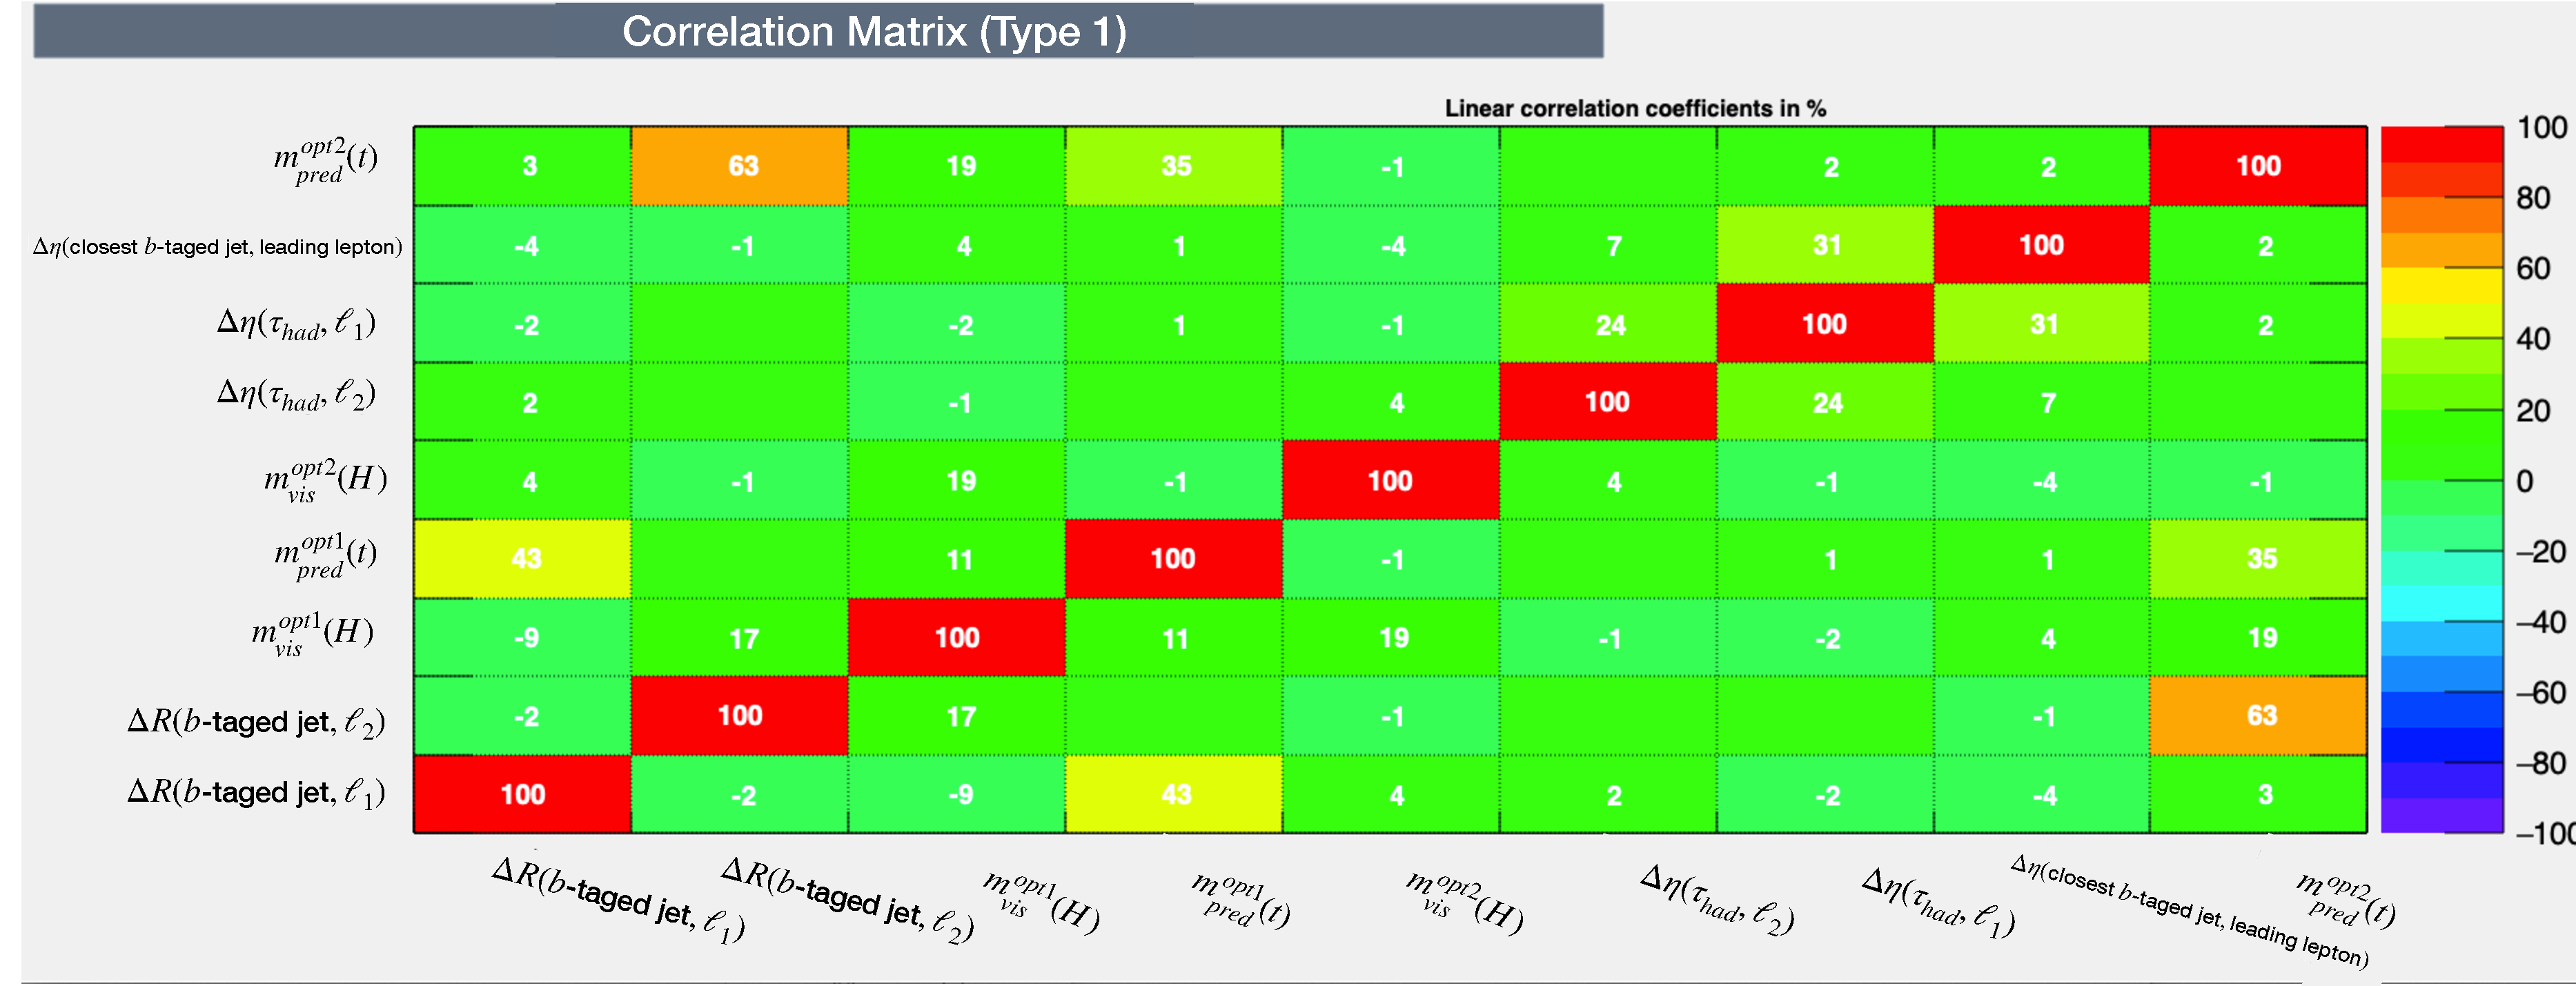
\includegraphics[width=1\linewidth]{Chapter5_tHq/LeptAssociation/BDT_InputVariables/pdf_0_input_correlations_Type1}
   \caption{Events with $\ell_{1}$ from the top quark and $\ell_{2}$ from the Higgs boson.}
   \label{fig:dileptau:Assignment_appendix:InputVars:Correlations:Type1} 
\end{subfigure}
\begin{subfigure}[b]{0.8\textwidth}
   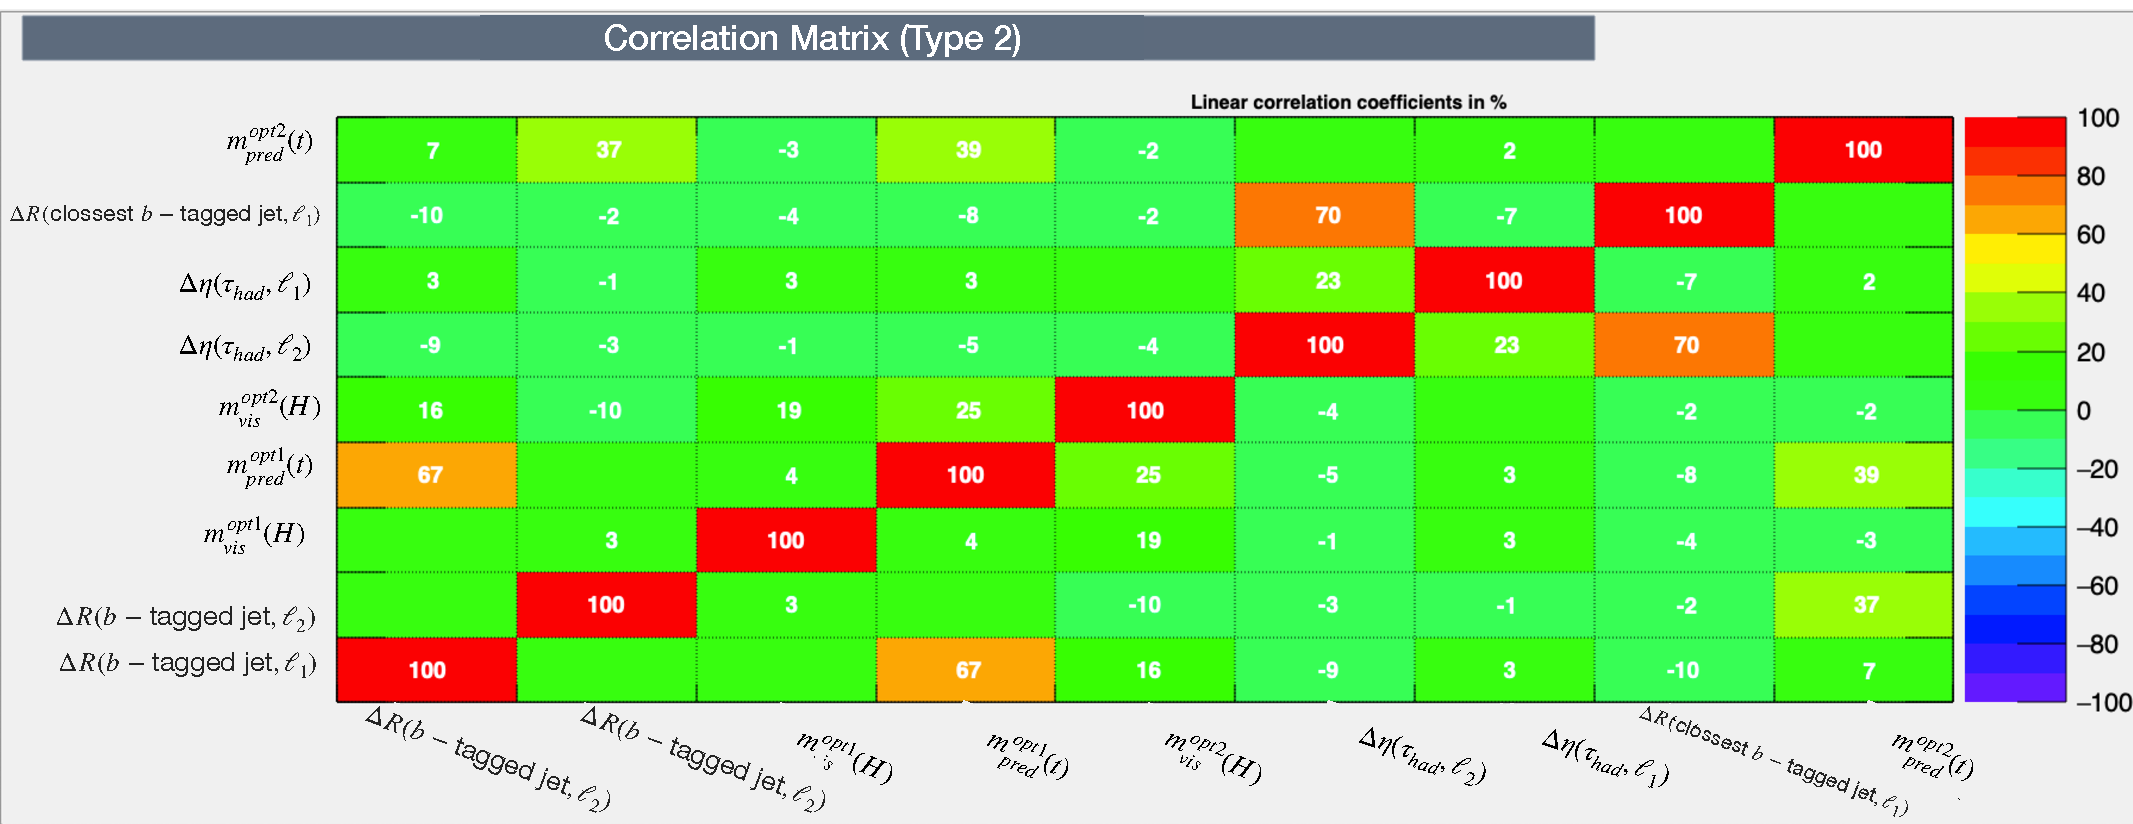
\includegraphics[width=1\linewidth]{Chapter5_tHq/LeptAssociation/BDT_InputVariables/pdf_0_input_correlations_Type2}
   \caption{Events with $\ell_{1}$ from the Higgs boson and $\ell_{2}$ from the top quark.}
   \label{fig:dileptau:Assignment_appendix:InputVars:Correlations:Type2}
\end{subfigure}
\caption{Matrices showing the linear correlation coefficients of the $\text{BDT}^{\text{Lepton Assignment}}$
 input variables for the Type$\,$1 
and Type$\,$2 samples. The correlation coefficients range from -100 to 100, being 0 the value for 
totally independent variables. Higher order functional or non-functional
relationships may not, or only marginally, be reflected in the value of linear correlation coefficient.}
\label{fig:dileptau:Assignment_appendix:InputVars:Correlations} %(See page 26 of the TMVA guide)
\end{figure}


%Numerous other variables were examined but were not integrated into the model due to several reasons.
%Some of these variables were not relevant in terms of separation power, while others displayed a strong correlation 
%with another variable that was already included in the model.

%Additionally, the decision to not incorporate additional input features into the model was influenced 
%by the fact that a separate BDT is used to distinguish between signal and background processes 
%(as described in Section~\ref{sec:ChaptH:EventSelection}). 

The list of variables used in the assignment BDT is chosen such that it does not overlap with that of the BDT 
trained to separate the signal from the background (Section~\ref{sec:ChaptH:EventSelection}). This is done in order
to avoid potential biases, since the input variables of the latter are built with the former.

%A reason not to incorporate more input features into the model is that 
%other BDTs are later trained and used for separating
%signal from the background processes (Section~\ref{sec:ChaptH:EventSelection}) as well as for designing the
%background enriched regions.
%These region-definition BDTs use
%as input the variable built with the assignment of leptons derived from the $\text{BDT}^{\text{Lepton Assignment}}$. 
%One shall be careful when doing this because
%using the same variables in both BDTs can lead to biases. 
%The region-definition BDTs are referred to as 
%BDT$(\tHq|_{\text{OS}})$, BDT$(\ttbar|_{\text{OS}})$ and BDT$(\tHq|_{\text{SS}})$,
%in contrast to the $\text{BDT}^{\text{Lepton Assignment}}$.
%This region-definition BDT includes variables that are built using the outcome of the $\text{BDT}^{\text{Lepton Assignment}}$
%and, hence, caution must be taken as double-using the same variables within a BDT can result in biases.


 %%%%%%%%%%%%%%%%%%
%           BDT-Hyperparameters     %
%%%%%%%%%%%%%%%%%%
\subsubsection{Optimisation of the lepton-assignment BDT hyperparameters}
\label{sec:ChaptH:Sig:LepAsign:SS:BDT:hyperparameters}
The hyperparameters are the parameters whose values control the learning process.
They are not part of the final model but determine the values of the model parameters that
the learning algorithm acquires. The values of the hyperparameters are optimised to maximise the 
performance of the assignment.
While certain ML libraries such as PyTorch, scikit-learn, XGBoost, and TensorFlow, 
offer functionality for discovering the most effective hyperparameter values, 
the corresponding capabilities within the TMVA  package of ROOT remain in a developmental stage, 
and presently, they are not even documented. Tests are carried to identify optimal 
hyperparameters using a grid-search-based algorithm, with the receiver operating characteristic (ROC) 
area serving as the primary figure of merit. 
However, better performances are achieved through the manual fine-tuning of hyperparameters.

A discussion about the different hyperparameters and their meaning is provided 
in the Appendix~\ref{fig:Appendix:BDT:Hyperparams}. The set of hyperparameters 
used to train the model is presented in Table~\ref{tab:chap:tH:LepAssign:Hyperparams}.

\begin{table}[htbp!]
\centering
\begin{tabular}{l|l|l}
\toprule
Hyperparam.	   			& Value  				& Meaning                               \\ 
\midrule
\texttt{Type} 				& Gradient      			& Boosting type for the trees.    \\
\texttt{MaxDepth} 			& 3      				& Maximum depth of cell tree.            \\
\texttt{Shrinkage}			& 0.2    				& Learning rate for GradBoost algorithm. \\
\texttt{NTrees}    			& $10^3$ 				& Number of trees in method.             \\
\multirow{2}{*} {\texttt{nCuts}} 	& \multirow{2}{*}{40} 		& Number of grid points in variable range used \\
		  				&					& in finding optimal cut in node splitting. \\
\bottomrule
\end{tabular}
\caption{Hyperparameters tuned for the $\text{BDT}^{\text{Lepton Assignment}}$ training. 
The rest of hyperparameters are set to its default values. 
More details about this can be found in Appendix~\ref{fig:Appendix:BDT:Hyperparams} or 
in Reference~\cite{TMVAUsersGuide}. The hyperparameter 
\texttt{NegWeightTreatment} is discussed in Section~\ref{sec:ChaptH:Sig:LepAsign:SS:BDT:NegWeights}.}
\label{tab:chap:tH:LepAssign:Hyperparams}
\end{table}

 %%%%%%%%%%%%%%
%        BDT-NegWeight     %
%%%%%%%%%%%%%%
\subsubsection{Treatment of the negatively-weighted events}
\label{sec:ChaptH:Sig:LepAsign:SS:BDT:NegWeights}
Negatively-weighted events can pose challenges when using a BDT or other ML techniques 
such as NN. These issues are discussed in more detail in Section~\ref{chap:Appendix:BDT:NegWeigts}.
The origin of the negatively-weighted events is explained in Appendix~\ref{chap:Appendix:NegWeights:intro}.

When training a BDT, it is necessary to address the issue of negatively-weighted events since the algorithm
cannot directly handle negative weights. Two common approaches to handle this situation are: 
ignoring negative weights during training and using the absolute values of the weights. 

In the case of ignoring negative weights during training, the BDT algorithm treats all 
events with negative weights as if they have zero weight (i.e. its information is lost). 
This approach avoids any potential complications arising from negative weights but 
still preserves the positively weighted events in the training process. On the other hand, 
using the absolute values of the weights involves taking the magnitude of the negative weights, 
effectively treating them as positive weights. This second strategy allows the BDT to 
incorporate the information from these events while disregarding the sign of the weights.

Other options are provided by the TMVA library of ROOT, as described in 
Section~\ref{chap:Appendix:BDT:NegWeigts:TMVARoot}. However, after conducting several tests, 
it is observed that these alternative techniques do not exhibit comparable performance 
in terms of both separation power and stability when compared to the approach of ignoring 
negative weights.

After careful evaluation and experimentation, it is determined that excluding events with 
negative weights yielded better results than using the absolute weights of the events. This 
approach demonstrated improved performance in terms of the desired outcomes of the
$\text{BDT}^{\text{Lepton Assignment}}$ training.

However, to ensure the validity of this approach, it should be verified that the subset of positively 
weighted events accurately represents the behaviour of the data. Approximately 40\% of the signal 
entries have negative weights and, hence, ignoring this subset could affect the distribution of the samples. 
Therefore, before discarding these events during training, it is necessary to examine whether the 
shape of the data distributions is significantly affected.

In the Figures in Appendix~\ref{chap:Appendix:BDT_Variables:LepAssignment}, I 
compare the shapes of the distributions
using all events versus using only positively weighted events. As shown, the variable distributions exhibit 
perfect compatibility within the error bands. Additionally, the concentration of negative weights is practically 
the same for both categories, with 36.1\% for Type$\,$1 and 36.6\% for Type$\,$2. This indicates a balanced
representation, as removing negative weights does not introduce bias towards either category.

In conclusion, using only the positively weighted events in the training 
process does not present any significant issue.





%%%%%%%%%%%%%
%           BDT-Training    %
%%%%%%%%%%%%%
\subsubsection{Training of the lepton-assignment BDT}
\label{sec:ChaptH:Sig:LepAsign:SS:BDT:Training}
The primary objective of the $\text{BDT}^{\text{Lepton Assignment}}$ is to differentiate 
between the Type$\,$1 and Type$\,$2 categories, similar to the separation 
of signal and background with the region-definition BDTs. %The variable 
%\texttt{isLep1fromTop} is used to label these categories. 
One important
difference between the region-definition BDTs and the $\text{BDT}^{\text{Lepton Assignment}}$
is that while the former are using all the samples, the latter is exclusively trained 
on \dilepSStau signal events. This approach is justified by the objective of 
determining the origin of each lepton in the signal events, a classification 
that is meaningful only within the context of signal processes

%Therefore, the two classes are define as:
%	\begin{itemize}
%		\item  \textbf{Type 1}: The leading $\ell$ (\emu) comes from the top-quark decay chain and, hence, 
%				the sub-leading from the Higgs boson (\texttt{isLep1fromTop} =0). 
%				As expected, this is the most frequent type since
%				the top quark carries more momentum. 
%		\item  \textbf{Type 2}: Just the opposite to the type 1. In this case, the decay chain 
%				of the Higgs boson is the source of the leading lepton while the sub-leading comes
%				from the top quark. The leading light lepton is a product from the Higgs-boson-decay chain
%				(\texttt{isLep1fromTop} =0).
%	\end{itemize}
 
The use of TMVA offers the advantage of directly 
working with the root-formatted NTuples, eliminating the need to 
convert them to numpy arrays or pandas dataframes.

%Nowadays most of ML frameworks (keras, pyTorch, scikit-learn, XGBooost, etc..) are based on python. 
%These libraries expect numpy arrays or panda data-frames as input, so the first thing to do 
%when using the analysis NTuples is to convert the ROOT data-frame. An advantage of using TMVA library of
%ROOT is that this data conversion is not necessary.

In order to mitigate the effects of low statistics, the \textit{k}-folding method (carefully described in 
the Appendix~\ref{chap:Appendix:BDT:kfold}) from cross validation in implemented using five folds. 
Thus meaning that the data is split in five sub-sets named folds 
and five BDTs are trained. Each model uses four folds
for training and one for test, implying that for each BDT the train/test split is 80/20\%.
After removing the negatively-weighted events, 9362 raw-events are used for building the model.
Of those 5518 are Type$\,$1 and 3844 Type$\,$2. Therefore, each of the five BDTs uses 7490 events
in the training and 1872 in the classification.
This cross-validation technique allows to use all the events in the dataset for the train. 
No validation dataset is used but the different models
are compared and if all of them behave similarly, there is no overtraining. 
%The node splitting stops once it has reached the minimum number of events which is specified in the
%BDT configuration, which is set to 100 by default.
% The default loss function used for AdaBoostR2Loss is "Quadratic"

 Due to the use of \textit{k}-folding, the training of the $\text{BDT}^{\text{Lepton Assignment}}$ results 
 in five distinct ML models. If overtraining had occurred, these models would not 
 generalise effectively, leading to noticeable differences in the BDT score\footnote{The 
 score of the BDT is the result of the model prediction for a given event.} distributions 
 between models. Therefore, it is crucial to ensure that the models are consistent 
 with one another.
 
 \begin{figure}[h]
	\begin{subfigure}[h]{0.5\linewidth}
		\includegraphics[width=\linewidth]{Chapter5_tHq/LeptAssociation/dileptau_LepAssignment_BDT_Score_ALL_train_GoodLegend.pdf}
		\caption{Events when used in the training set.}
	\end{subfigure}
	\hfill
	\begin{subfigure}[h]{0.5\linewidth}
		\includegraphics[width=\linewidth]{Chapter5_tHq/LeptAssociation/dileptau_LepAssignment_BDT_Score_ALL_test_GoodLegend.pdf}
		\caption{Events when used in the test set.}
	\end{subfigure}%
	\caption{Comparison of the profiles of the  $\text{BDT}^{\text{Lepton Assignment}}$ scores for the different models (folds). 
	Observe that the scores exhibit similar distribution shape, indicating that 
	the model is not affected by the particular subset of data used for training.}
	\label{fig:ChaptH:dileptau:Assignment:ScoreDistributions}
\end{figure}

Figure~\ref{fig:ChaptH:dileptau:Assignment:ScoreDistributions} displays the BDT 
score distributions for all five folds simultaneously. The purpose of this visualisation 
is to assess the compatibility of the five models and verify the absence of overtraining. 
As observed in the figure, the BDT score distributions are consistent across the folds, 
indicating that there is no evidence of overtraining.


Additionally, it is essential to compare the distributions of the train and test 
samples for each model. The greater the similarity between these distributions, 
the better the model's performance. However, it is crucial to note that an exact 
agreement between the train and test samples could indicate a potential bug or 
issue with the model.
Figure~\ref{fig:dileptau:Assignment_appendix:ScoreDistributions:Example}
presents, for a single model, the $\text{BDT}^{\text{Lepton Assignment}}$ simultaneously displaying 
the train and test samples while distinguishing between the two event types.
The train versus test plots of the models corresponding to the other folds, 
are in Figure~\ref{fig:dileptau:Assignment_appendix:ScoreDistributions}
of Appendix~\ref{chap:Appendix:BDT}.
By examining the figure, it can be 
observed that the train and test samples exhibit compatibility, indicating that the 
models are performing well and are not overfitting to the training data.


\begin{figure}[h]
\centering
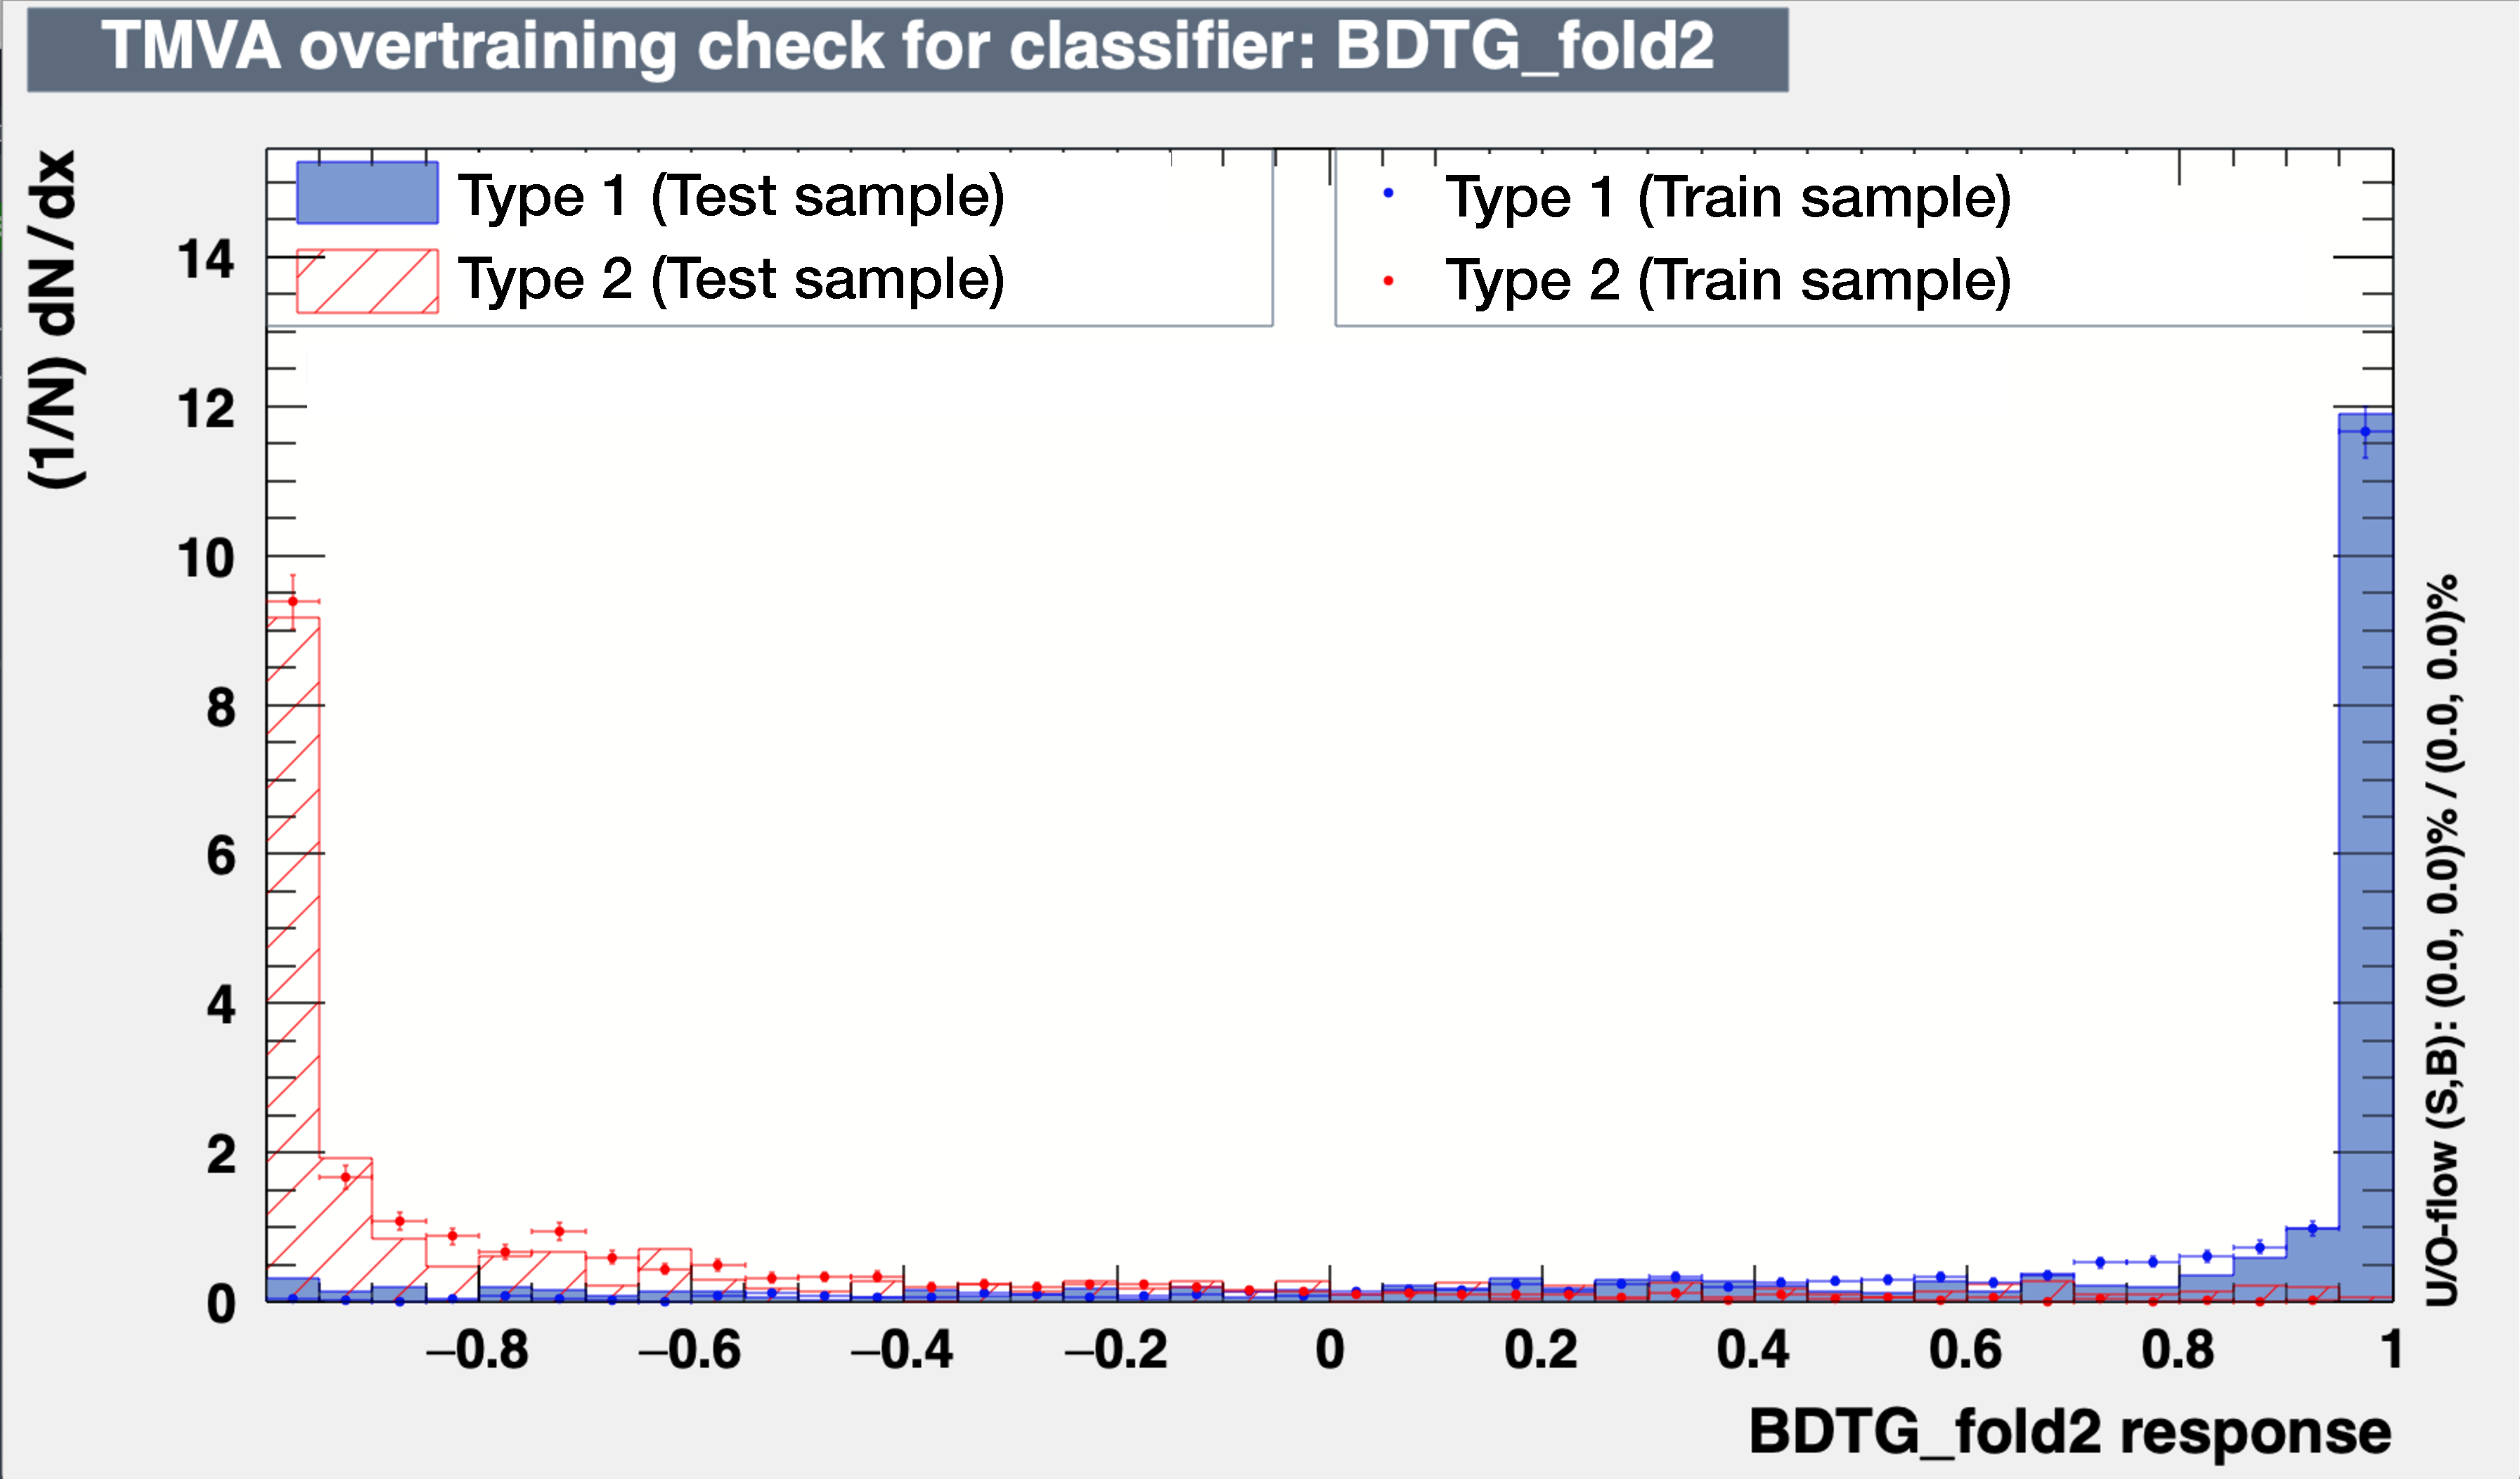
\includegraphics[width=.7\textwidth]{Chapter5_tHq/LeptAssociation/Dileptau_BDT_Based_Assignment_Score_Fold2}
\caption{$\text{BDT}^{\text{Lepton Assignment}}$ distributions for test and train samples superimposed in one of the folds.}
\label{fig:dileptau:Assignment_appendix:ScoreDistributions:Example}
\end{figure}


Figures~\ref{fig:dileptau:Assignment:ROC_and_Score:ROC} and 
\ref{fig:dileptau:Assignment:ROC_and_Score:Score} present the 
ROC curve and BDT score, respectively, separated by categories and 
combining the data from all five folds. The ROC curve illustrates the 
balance between correctly identifying Type$\,$1 instances and misclassifying 
Type$\,$2 instances at various classification thresholds. A higher ROC 
curve and a larger area under the ROC curve (AUC) indicate improved 
classification performance. A more comprehensive explanation of these 
concepts can be found in Appendix~\ref{chap:Appendix:BDT:Concepts}. 
Notably, the Type$\,$1 and Type$\,$2 categories replace the conventional 
positive and negative instances. The substantial AUC observed in the ROC 
curve signifies strong performance. For a detailed view of the ROC curves for
each fold individually, refer to Figure~\ref{fig:dileptau:Assignment_appendix:ROCs}
in the Appendix~\ref{chap:Appendix:BDT}.

Regarding the $\text{BDT}^{\text{Lepton Assignment}}$
 score in Figure~\ref{fig:dileptau:Assignment:ROC_and_Score:Score}, 
it is evident that the Type$\,$1 and Type$\,$2 categories exhibit distinct peaks at opposite 
extremes of the distribution. This significant separation confirms the effectiveness of the 
$\text{BDT}^{\text{Lepton Assignment}}$
 when differentiating between the two categories. It is worth noting that in Figure~\ref{fig:dileptau:Assignment:ROC_and_Score:Score}, the bullets 
representing the train sample and the shadowed area representing the test samples 
appear identical due to the way TMVA combines the folds in a single histogram. 
However, the accurate assessment of the test versus train comparison is shown in Figure~\ref{fig:dileptau:Assignment_appendix:ScoreDistributions}.

\begin{figure}[h]
  \begin{subfigure}[h]{0.51\linewidth}
  	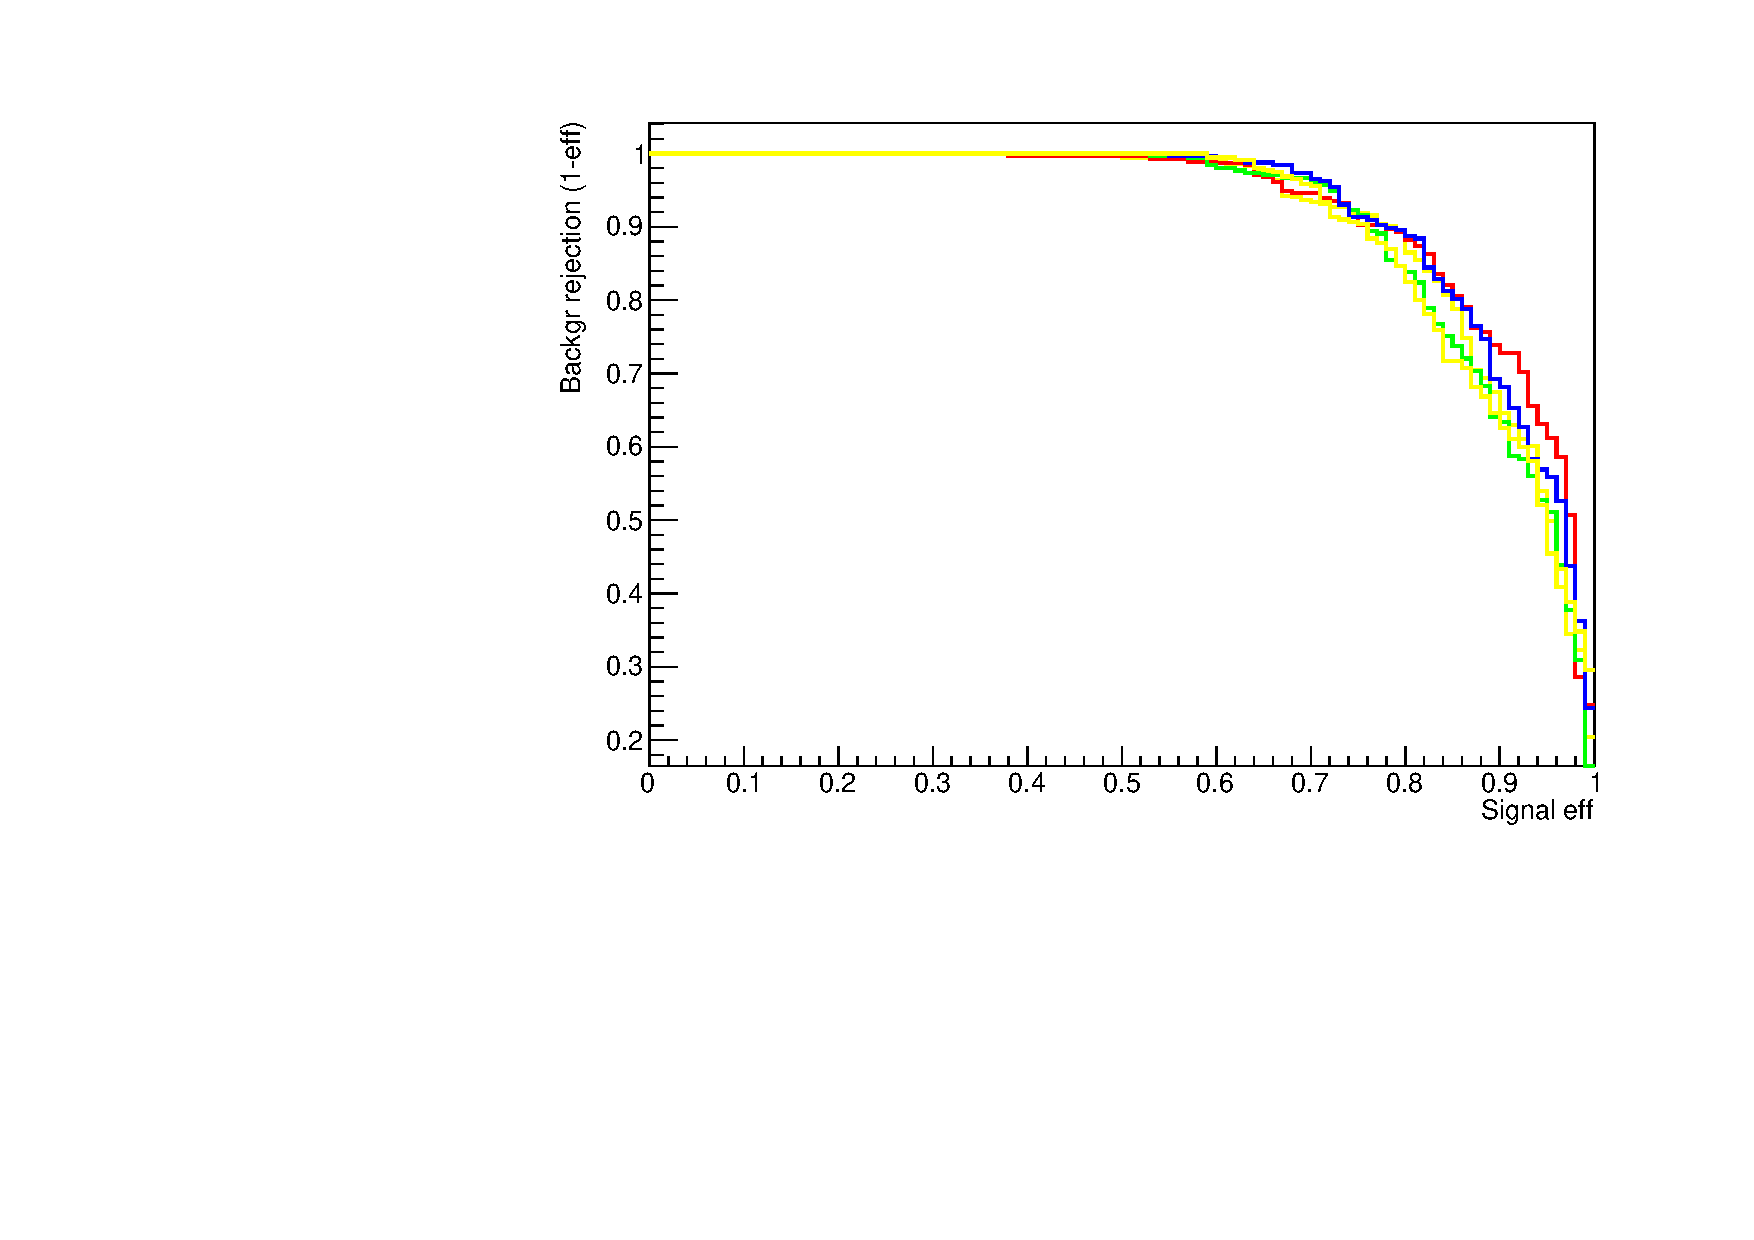
\includegraphics[width=\linewidth]{Chapter5_tHq/LeptAssociation/LeptonAssignment_roc_curves}
	\caption{ROC curve}
	\label{fig:dileptau:Assignment:ROC_and_Score:ROC}
  \end{subfigure}
  %\hfill
  \begin{subfigure}[h]{0.49\linewidth}
	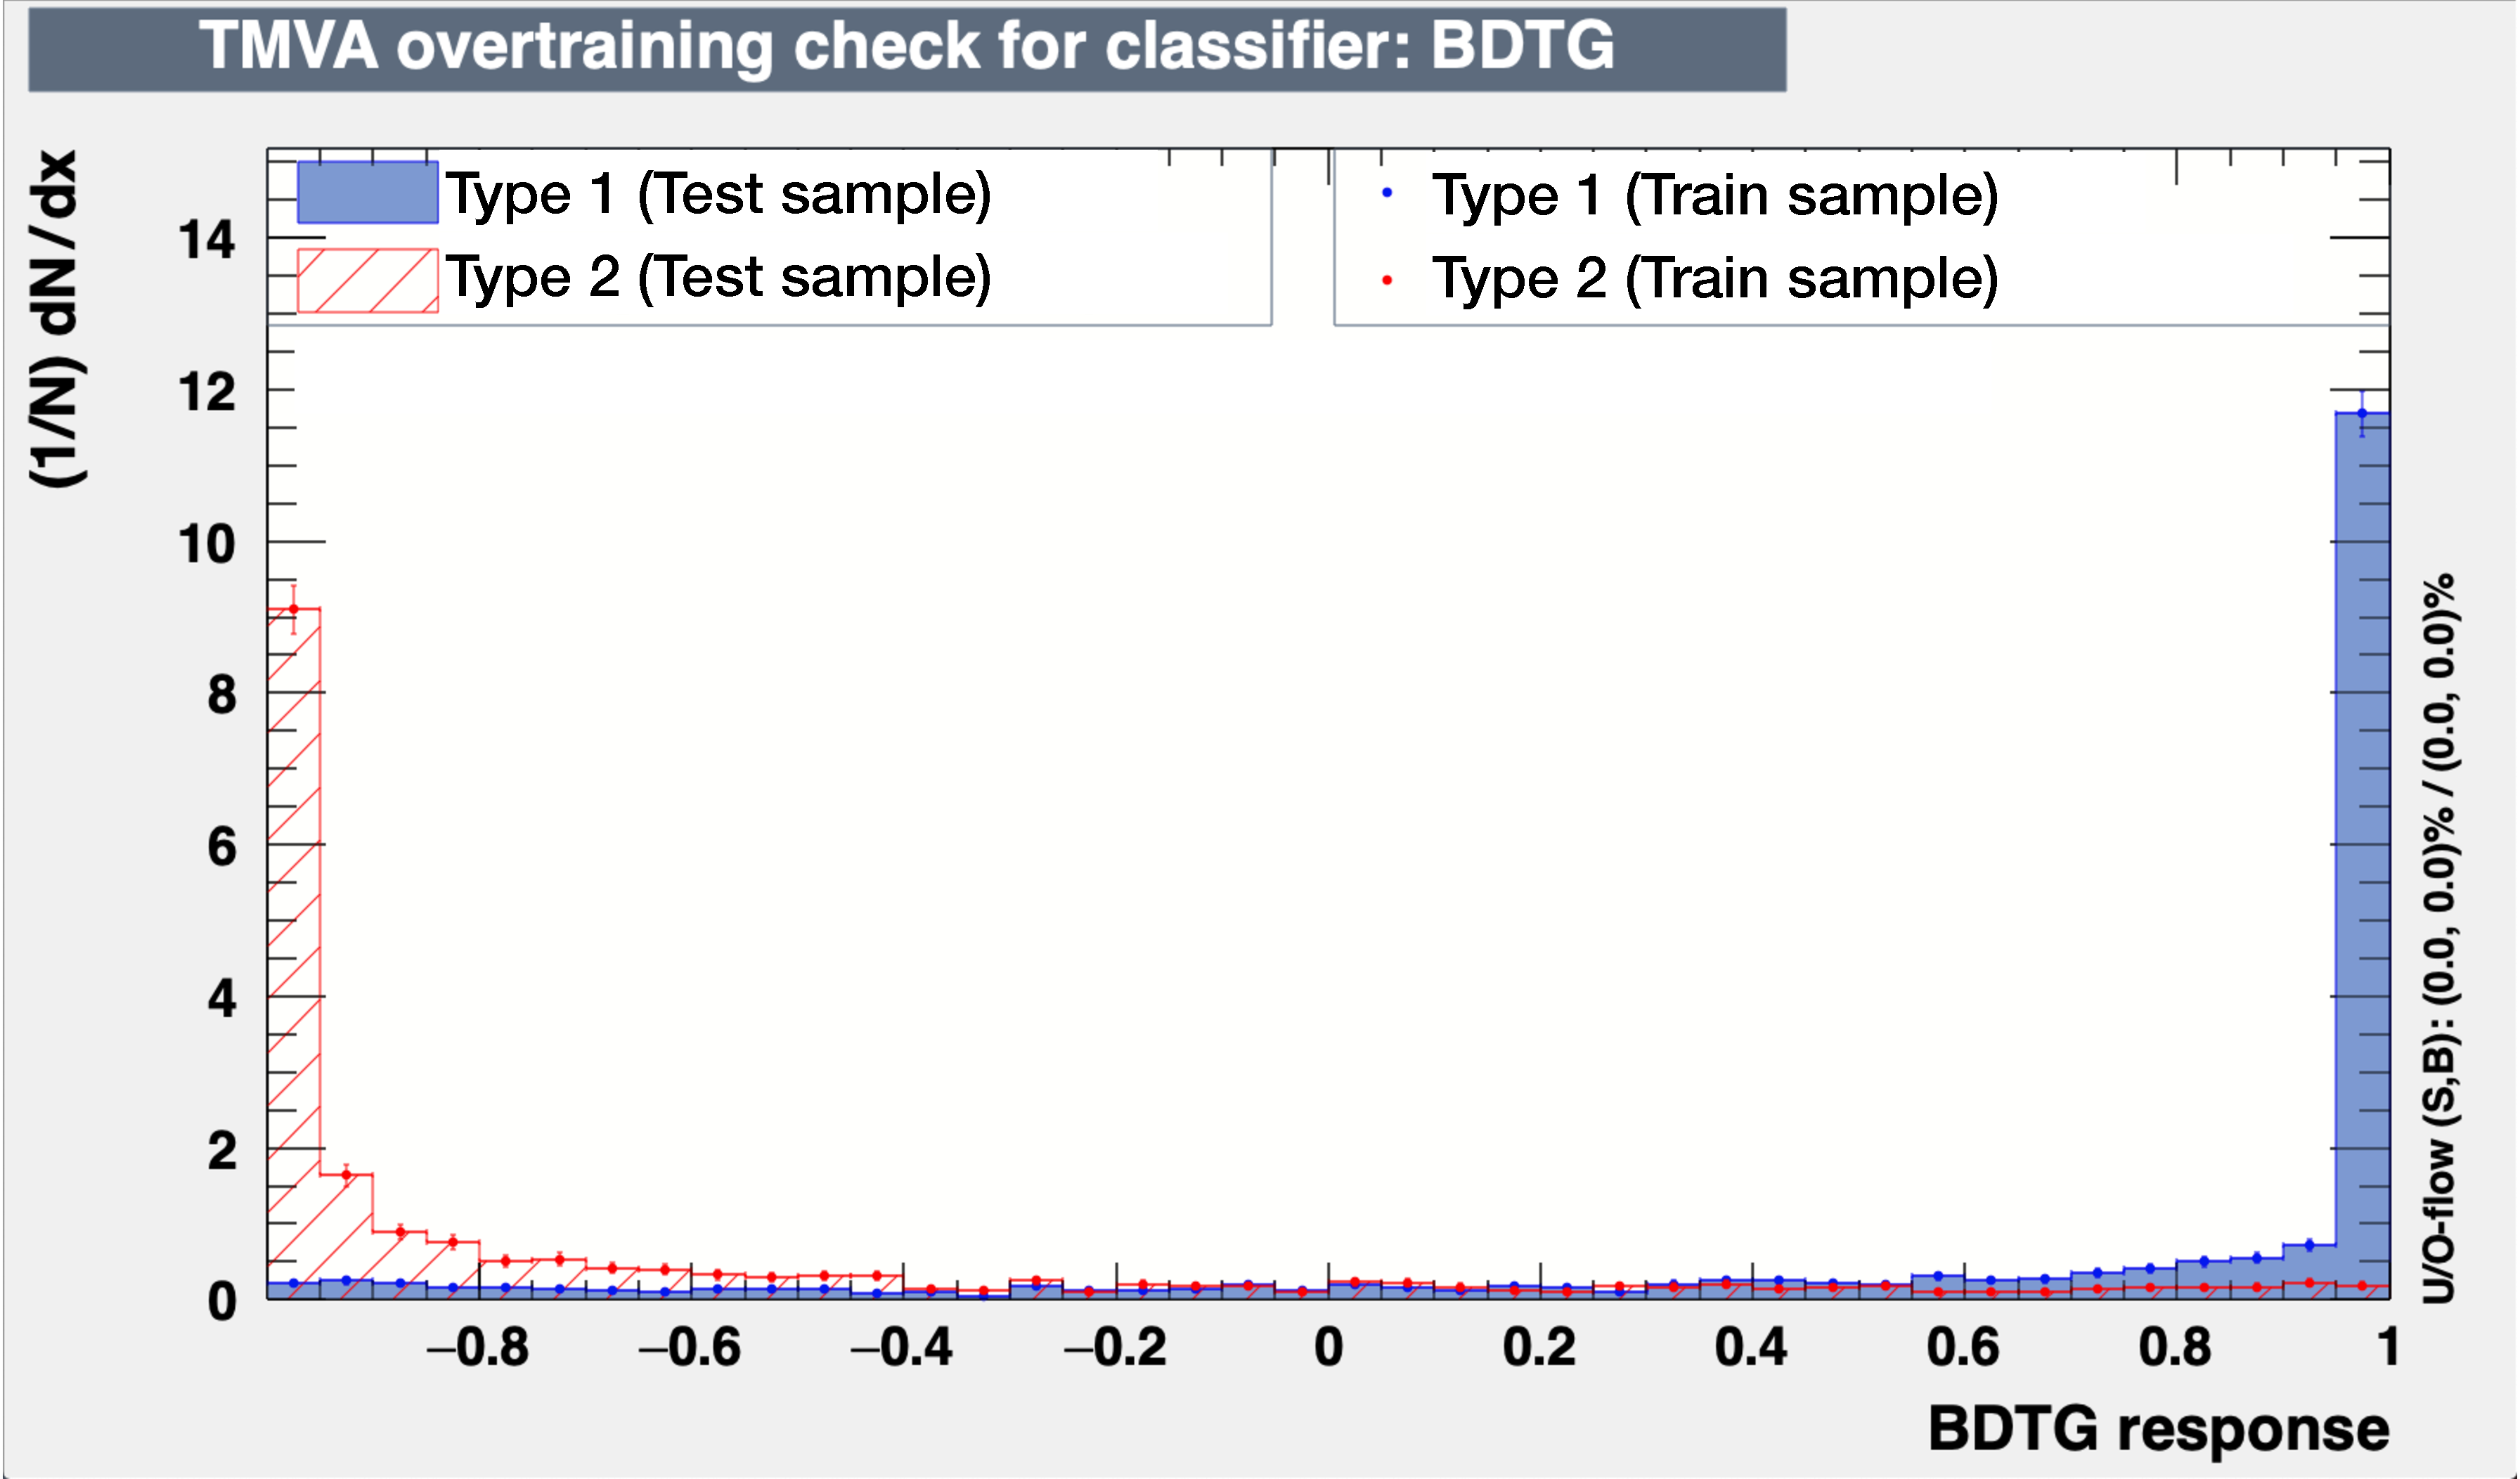
\includegraphics[width=\linewidth]{Chapter5_tHq/LeptAssociation/Dileptau_BDT_Based_Assignment_Score_General}
	\caption{BDT score} 
	\label{fig:dileptau:Assignment:ROC_and_Score:Score}
  \end{subfigure}%
\caption{ROC (a) and score (b) combining all folds for the $\text{BDT}^{\text{Lepton Assignment}}$.
Each curve in (a) represents a different fold. Note the small discrepancies between them. }
\label{fig:dileptau:Assignment:ROC_and_Score}
\end{figure}
		 
%\pablo{Faltan los plots (si existiesen, que no existen) de la logloss.}

 %%%%%%%%%%%%%%%%%%
%           BDT-Thereshold     %
%%%%%%%%%%%%%%%%%%
\subsubsection{Model application and classification-threshold selection}
\label{sec:ChaptH:Sig:LepAsign:SS:BDT:Application}


Although the model-building tool is developed as an independent 
and self-contained application, the $\text{BDT}^{\text{Lepton Assignment}}$
model is integrated into the \thqloop framework. As a result, during the production 
of post-processed NTuples (i.e. the \thqloop output), the lepton origin in the 
\dilepSStau is already used for variable construction. 
This represents a great advantage since it simplifies the post-processing of NTuples.
%It is important to note 
%that this procedure differs from the approach employed in the BDT for region 
%definition discussed in Section~\ref{sec:ChaptH:EventSelection}. In the latter BDT, 
%the scores are injected separately within a distinct framework.

Since \textit{k}-folding is used, there are several models and, hence, it is necessary to define a 
criteria to decide which model apply to each event. On the one hand, for the events used in the training, the BDT
used is the one in which that event was part of the test sample. On the other hand, for the events
that do not take part in the training, the choice of BDT is randomised using the variable \texttt{event number}.
Since the event number has no physical meaning, it is equivalent to randomly assigning a BDT to each event. 


Note that the $\text{BDT}^{\text{Lepton Assignment}}$
output is not a category but a real number ($\text{BDT}^{\text{Lepton Assignment}}$). To define
to which category assign the event, a threshold value is selected. All the events
with $\text{BDT}^{\text{Lepton Assignment}}$ scores above the selected threshold are classified as  Type$\,$1
and, contrary, if the BDT score is below as Type$\,2$. 
A search of the optimal threshold is presented in Table~\ref{tab:dileptau:Assignment_appendix:Thereshold}
and $\text{BDT}_{\text{Threshold}}^{\text{Lepton Assignment}} = -0.315$ is the best value for 
separating the two categories.


\begin{table}[h]
\centering
\resizebox{\textwidth}{!}{
\begin{tabular}{l|lllllllll}
\toprule
$\text{BDT}_{\text{Threshold}}^{\text{Lepton Assignment}}$    & -0.45 & -0.4  & -0.35 & -0.33 & -0.32 & -0.315 & -0.31 & -0.395 & -0.3  \\ \midrule
Accuracy (\%) & 88.12 & 88.03 & 87.97 & 88.23 & 88.33 & 88.39  & 88.36 & 88.32  & 88.15 \\ \bottomrule
\end{tabular}}
\caption{Different studied $\text{BDT}^{\text{Lepton Assignment}}$ thresholds 
compared to its correspondent accuracy.
The first row is the value on the lepton-assignment-BDT-score threshold 
($\text{BDT}_{\text{Threshold}}^{\text{Lepton Assignment}}$) 
that is used to separate between 
Type$\,$1 and Type$\,$2 events. If for an event the score is larger than threshold value, the 
leading lepton is considered to come from the top quark. The accuracy on the second row is calculated
using the truth-level information.}
\label{tab:dileptau:Assignment_appendix:Thereshold}
\end{table}


 %%%%%%%%%%%%%%%%%%
%           BDT-Results    %
%%%%%%%%%%%%%%%%%%
\subsubsection{Results of the BDT-based method for lepton assignment}
\label{sec:ChaptH:Sig:LepAsign:SS:BDT:Results}


The result obtained by this method can be compared to the one given by the cut-based alternative method 
described at the beginning of this Section. A summary of the performance of the two methods
is given in Table~\ref{tab:dileptau:Assignment:MethodsSummary}.
As Table~\ref{tab:dileptau:Assignment:MethodsSummary} shows, the performance of the BDT-based method
method surpasses that of the alternative approaches.

\begin{table}[h]
\centering
\resizebox{\textwidth}{!}{
\begin{tabular}{l|llc|}
\cline{2-4}
 & \multicolumn{3}{c|}{Accuracy of the light-lepton-origin assignment} \\ \cline{2-4} 
                                       & \multicolumn{1}{l|}{Total (100\%)} & \multicolumn{1}{l|}{$H\rightarrow \tau \tau$ (83.08\%)} & $H\rightarrow WW$ (16.92\%) \\ \midrule
\multicolumn{1}{|l|}{BDT-based method} & \multicolumn{1}{c|}{88.39}         & \multicolumn{1}{c|}{88.44}             & 88.18         \\ \midrule
\multicolumn{1}{|l|}{Cut-based method}       & \multicolumn{1}{c|}{83.86}         & \multicolumn{1}{c|}{84.24}             & 81.80         \\ \bottomrule
\end{tabular}}
\caption{Accuracy calculated by comparing the prediction of the method to the true value. 
The true value has been obtained using the labelling described in Section~\ref{sec:tHq:origin:LeptonAssignment_truth_reco_DeltaRCone}. 
This labelling is only available for \Htautau and \HWW. Only the events with successful reconstruction-level and truth-level matching
are used to produce the table.
From these events, 83\% are \Htautau and 17\% \HWW. The NN-based initial approach is not presented since it does not have any proper labelling.}
\label{tab:dileptau:Assignment:MethodsSummary}
\end{table}

 
 
%\subsubsection{[Borrar] Las movidas que no quiero olvidar decir}
%\begin{itemize}
%	\item Compare to the results using other MVA methods.
%	\item The BDT is integrated in \thqloop (weights.xml) ¿Where do I describe what \thqloop is?
%	\item From \thqloop, the BTD score can be calculated for all the events (signal or not) and then 
%	the efficiency of the lepton association can be calculated depending on the threshold point which is
%	chosen to define whether the event is Type$\,$1 or Type$\,$2. Note that this efficiency is computed only over
%	signal events. $\rightarrow$ Table of 'efficiency vs cutpoint'
%	
%	\item \textbf{Result}: 
%		\begin{itemize}
%			\item ROC curves for all folds in Figure~\ref{fig:dileptau:Assignment_appendix:ROCs}
%			\item Table~\ref{tab:dileptau:Assignment_appendix:Thereshold} is exploring classification 
%			accuracies depending on which BDT-score point is used to separate type1 and type 2.	
%		\end{itemize}
%\end{itemize}



%%%%%%%%%%%%%%%%%%%%%%%%%%%%
%           Top quark and Higgs boson reconstruction      %
%%%%%%%%%%%%%%%%%%%%%%%%%%%%
\subsection{Reconstruction of the top quark and the Higgs boson}
\label{sec:ChaptH:Sig:EventReconstruction} 
% Source: Presentation on 14/10/2020
%.              https://www.overleaf.com/project/5f74653051c93a00018b5f95
In order to suppress background events, it is desirable to reconstruct the 
kinematics of both the top quark and the Higgs boson. 
%By doing this, it is possible to define variables that can further separate the signal.
The accurate reconstruction of these particles is a challenging task 
due to the presence of four neutrinos in the final state, of which at least three 
are from the Higgs boson and one is from the top quark\footnote{This is 
assuming the most common decay channel, \Htautau.}. 
In this work, the strategy used to fully reconstruct the top and the Higgs boson consists on first
reconstructing the top-quark system and, then, the Higgs-boson chain. Since we know
the total \MET, if the missing energy is reconstructed for the top quark, 
it is possible to access the $\overrightarrow{E}_{\text{T}}^{\text{miss}} (\text{Higgs})$ based on:
\begin{equation*}
	\overrightarrow{E}_{\text{T}}^{\text{miss}} (\text{total}) = \overrightarrow{E}_{\text{T}}^{\text{miss}} (\text{Higgs}) + \overrightarrow{E}_{\text{T}}^{\text{miss}} (\text{top}) \,.
\end{equation*}

The possible final-state configurations when the Higgs boson decays to $\Ptauon \APtauon$ are described in Table~\ref{tab:ChaptH:Reconstruction:Configurations}.
The first two final-state columns in this table represent 92.7\% of \Htautau events 
while the last one can be neglected. This means that it is a relatively safe option to assume that
the \tauhad is produced from the decay of the Higgs boson.
This has been calculated from the numbers in Table~\ref{tab:ChaptH:TruthSummary}.
%These two columns represent the scenario in which the \tauhad comes from the \PHiggs.
This particular decay form of the \tHq(\dileptau) production is presented in the Feynman diagram of
Figure~\ref{fig:tHq:TruthFeyman}. 


\begin{table}[h]
\centering
\begin{tabular}{l|l|l|l|l}
\toprule
 $q$ & $q$ & jet & jet & jet \\ \midrule
 $H$ & $\tau$ & $\tauhad \: \nu_{\tau}$           &  $\tauhad \: \nu_{\tau}$           & $\Plepton_1 \: \nu_{\Plepton_1} \: \nu_{\tau}$ \\ 
     & $\tau$ & $\Plepton_1 \: \nu_{\Plepton_1} \: \nu_{\tau}$ &  $\Plepton_2 \: \nu_{\Plepton_2} \: \nu_{\tau}$ & $\Plepton_2 \: \nu_{\Plepton_2} \: \nu_{\tau}$ \\ \midrule
 $t$ &  $W$   & $\Plepton_2 \: \nu_{\Plepton_2}$               &  $\Plepton_1 \: \nu_{\Plepton_1}$               &  $\tauhad \: \nu_{\tau}$          \\ %\hline
     &  $b$   &  $b$-jet                         &  $b$-jet                          & $b$-jet                          \\ \bottomrule
\end{tabular}
\caption{Possible configurations of the final state objects in the \dileptau channel when the Higgs boson decays
to \tauhad and \taulep. The first column presents the spectator quark $q$, the \PHiggs boson and the \Ptop quark.
The second column shows the \PHiggs and \Ptop decays. The other three columns show the different possible configurations in 
which these objects can further decay.}
\label{tab:ChaptH:Reconstruction:Configurations}
\end{table}


\begin{figure}[h]
\centering
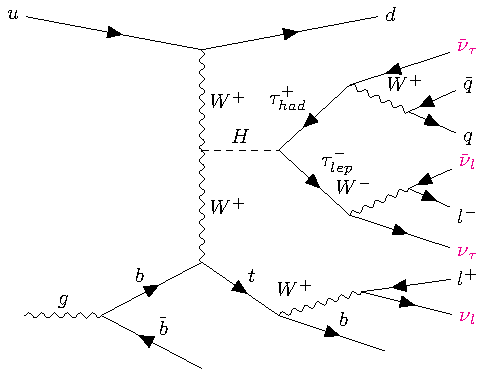
\includegraphics[width=.7\textwidth]{Feynman_diagrams/Feynman_tHq_Htautau_4Neutrinos}
\caption{Representative LO Feynman diagram for the \tHq (\dileptau) in 
the $\PHiggs \rightarrow \tauhad \taulep$ decay channel. The presence of the four neutrinos 
that complicates the reconstruction is 
highlighted in magenta.}
\label{fig:tHq:TruthFeyman}
\end{figure}

Before reconstructing the top quark or Higgs boson, the two charged-light leptons in the final state have to be
assigned to their corresponding parent. In most of cases, one $\Plepton$ comes from the Higss and the other 
from the top. %The origin association is described in detail in Section~\ref{sec:ChaptH:Sig:LepAsign}.

%%%%
%.  Top quark reconstruction
%%%
\subsubsection{Reconstruction of the top quark}
\label{sec:ChaptH:Sig:EventReconstruction:top}
To reconstruct the top quark, it is essential to have complete knowledge of the 4-momentum of both 
the $\PW$ boson and the $\Pbottom$ quark. %However, the reconstruction of the $\PW$-boson decay presents a 
%significant challenge due to the kinematics of the neutrino, which escapes the detector without being detected.
Therefore, if the neutrino is reconstructed, the top system can be reconstructed as well. 

%The objective is to obtain the $\overrightarrow{E}_{\text{T}}^{\text{miss}}$ of the top-quark system, 
%for which it is sufficient\footnote{Determining $p^{z}_{\Pnu}$ would add a constrain in the system of equations to solve the system
%and, hence, it would be 
%possible to get exact solutions for al the components of $\overrightarrow{p}(\Pnu_{\text{top})}$.}
To properly reconstruct the top quark it is necessary
 to determine the z-component of the neutrino momentum, \pnutopz. 
In order to achieve this, various hypotheses are examined using parton-level information
to derive \pnutopz from the z-component momentum of $\ell_{\text{top}}$.
One of the initial hypotheses tested was whether the z-component of the neutrino momentum in the top-quark system 
exhibits a linear dependence with a coefficient $\alpha$ on the z-component of the momentum of the light lepton, $p_{z}(\ell_{\text{top}})$. 
Being the parameter $\alpha$ a real number ranging from -1 to 1, the hypothesis $p^{z}(\Pnu_{\text{top}}) = \alpha \cdot p^{z}(\ell_{\text{top}})$
is tested in Figure~\ref{fig:tHq:EventReconstruction:TopSystem:hypothesis1}. 
%If  $\alpha=-1$, it would indicate aa back-to-back topology between $p_{z}(\ell_{\text{top}})$ and \pnutopz
%are compared 
This hypothesis was tested by studying the parton-level information of the top quark and its neutrino. The results indicate that the dependence between these two parts is not linear and, hence, this hypothesis for $p^{z}(\Pnu_{\text{top}})$ is not supported.
\begin{figure}[h] 
	\centering
	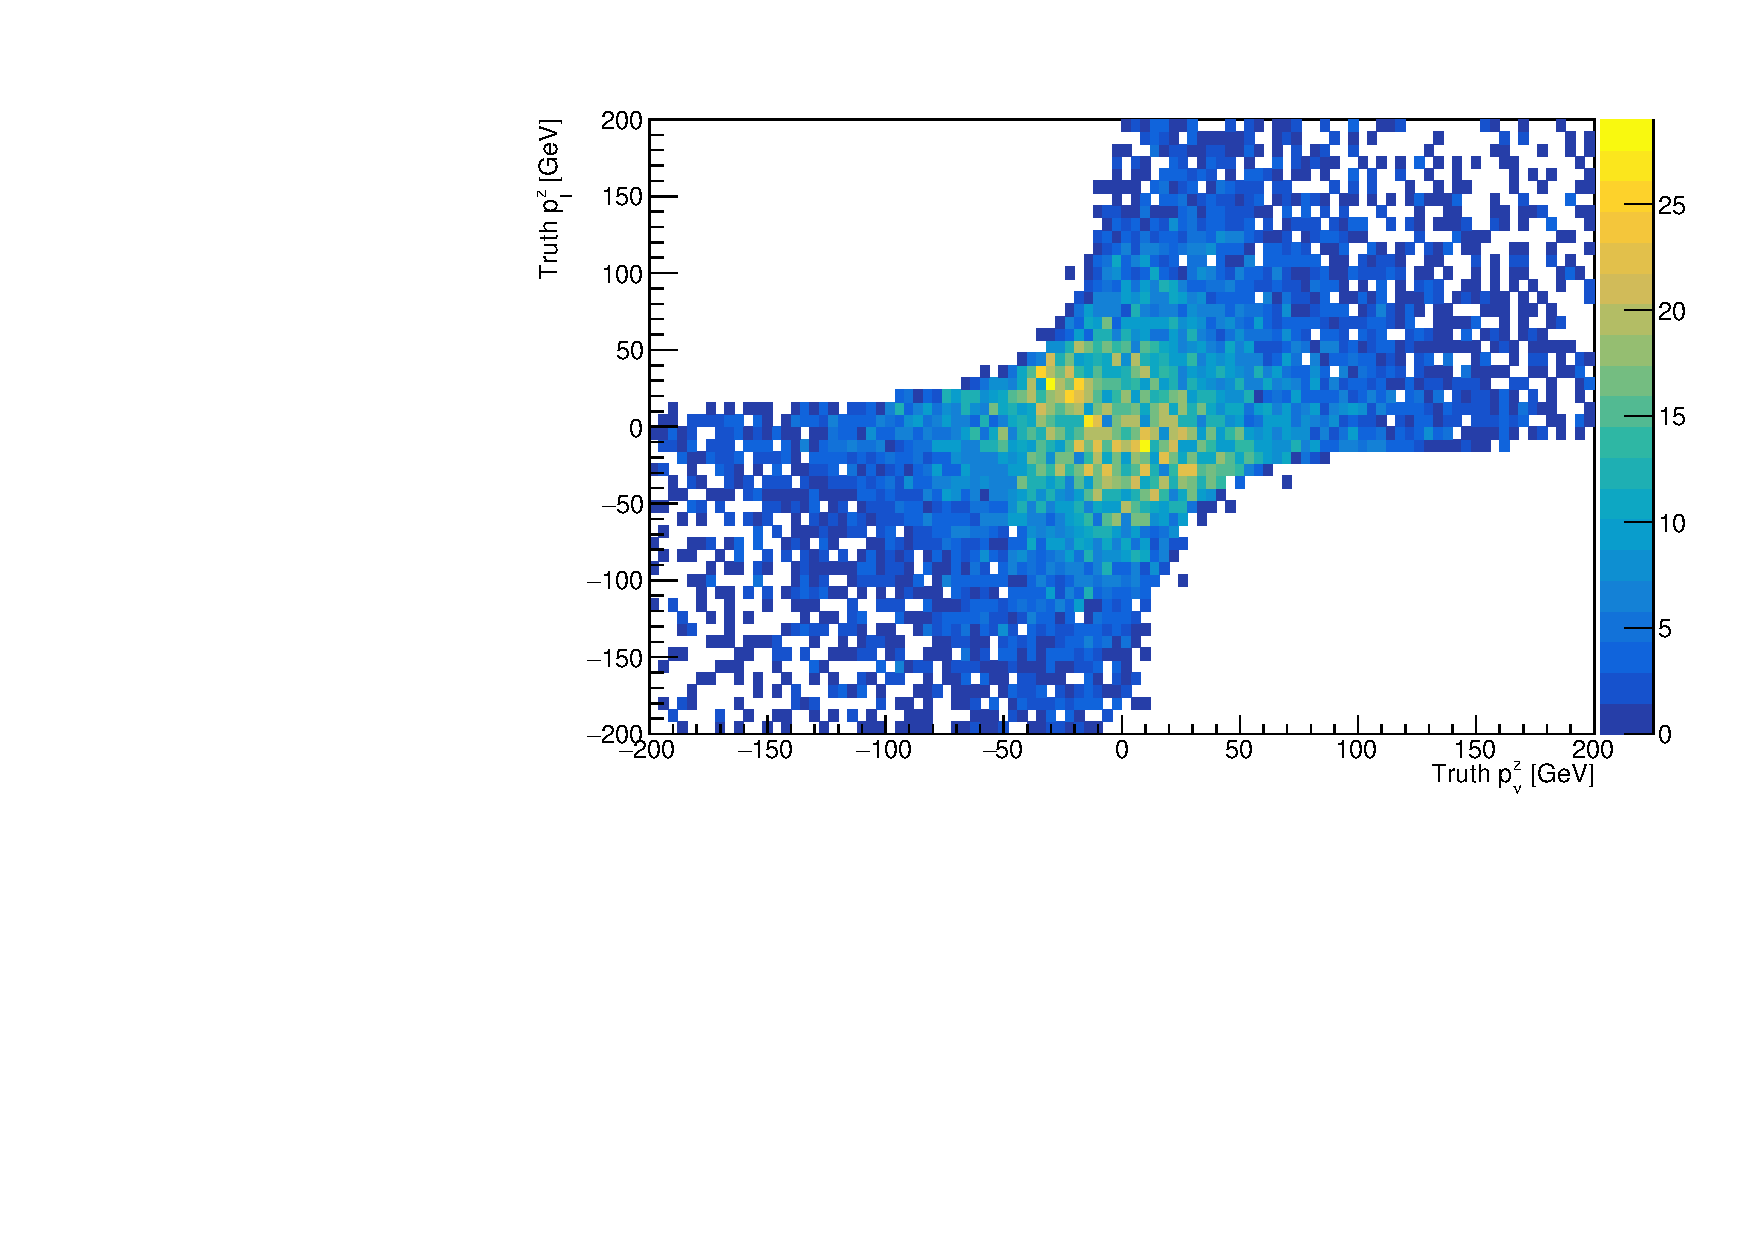
\includegraphics[width=0.55\linewidth]{Chapter5_tHq/Reconstruction/Pzv_vs_Pzl_truth_alp05}
	\caption{Distributions comparing $p_{z}(\ell_{\text{top}})$ and \pnutopz at 
	parton level to check if there is a dependence.}	
	\label{fig:tHq:EventReconstruction:TopSystem:hypothesis1}
\end{figure}

\begin{comment}
\begin{figure}[h] 
	\begin{subfigure}{0.45\textwidth}
	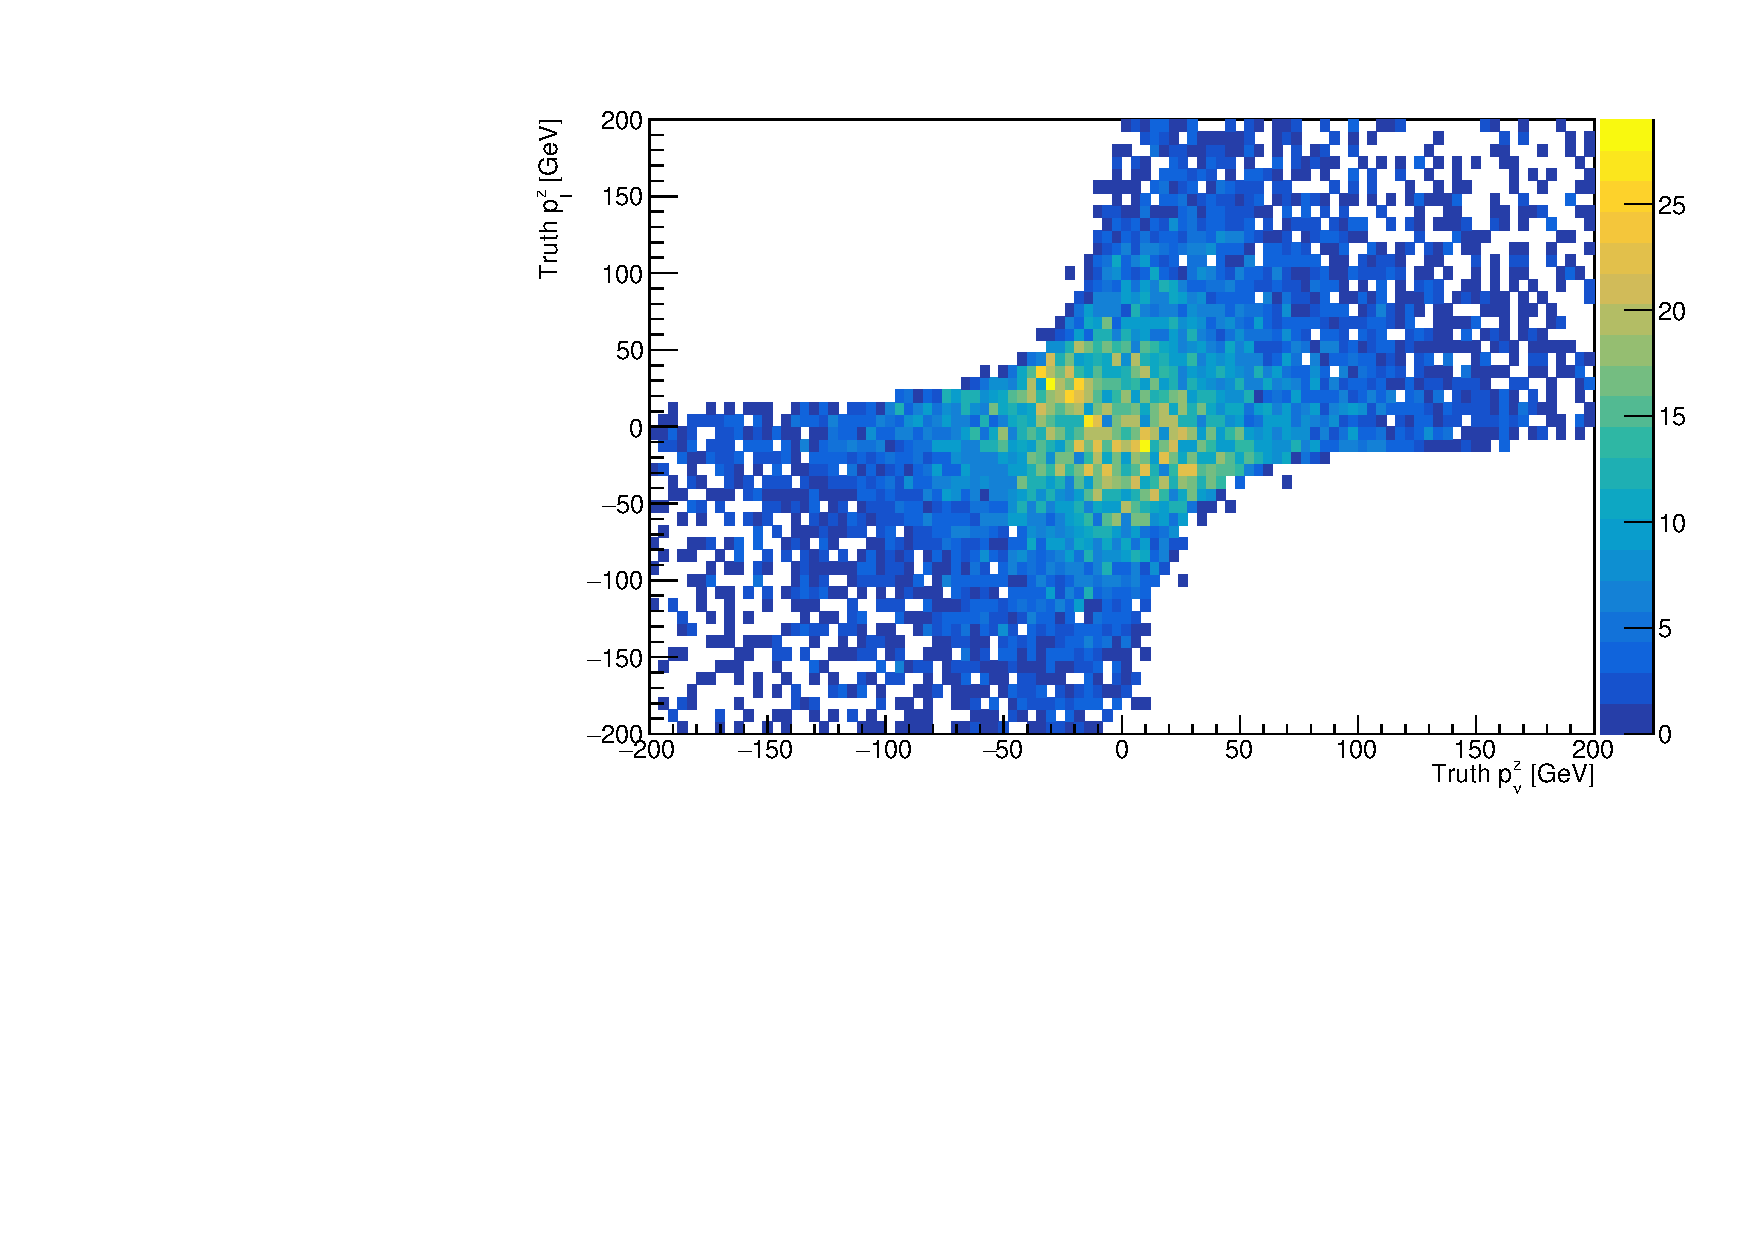
\includegraphics[width=\linewidth]{Chapter5_tHq/Reconstruction/Pzv_vs_Pzl_truth_alp05}
	\caption{Truth $p_{z}(\ell_{\text{top}})$ vs. Truth $p_{z}(\nu)$}
	\label{fig:tHq:EventReconstruction:TopSystem:hypothesis1:A}
	\end{subfigure}
\hfill 
	\begin{subfigure}{0.45\textwidth}
	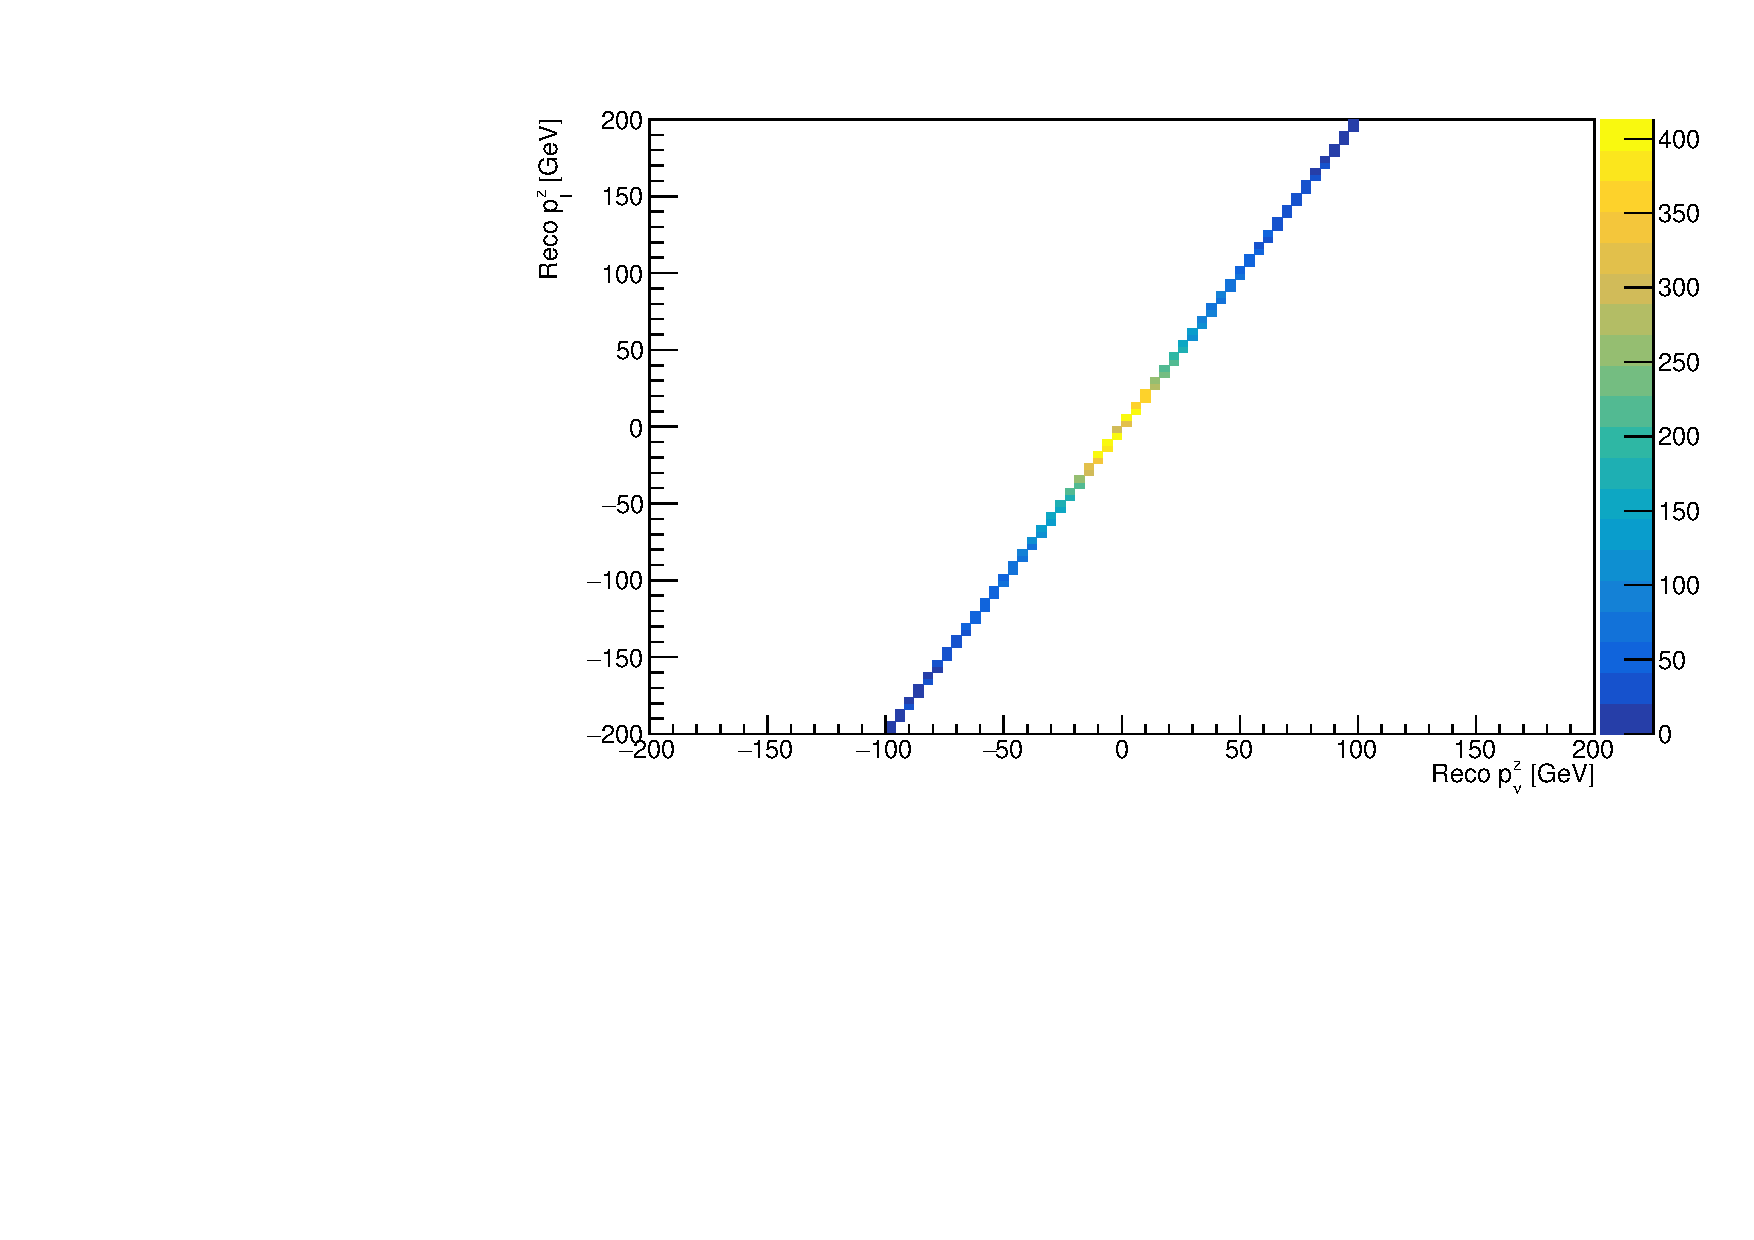
\includegraphics[width=\linewidth]{Chapter5_tHq/Reconstruction/Pzv_vs_Pzl_Reco_alp05}
	\caption{Reco. $p_{z}(\elll_{\text{top}})$ vs. Reco. \pnutopz}
	\label{fig:tHq:EventReconstruction:TopSystem:hypothesis1:B	}
	\end{subfigure}

\bigskip  
	\begin{subfigure}{0.45\textwidth}
	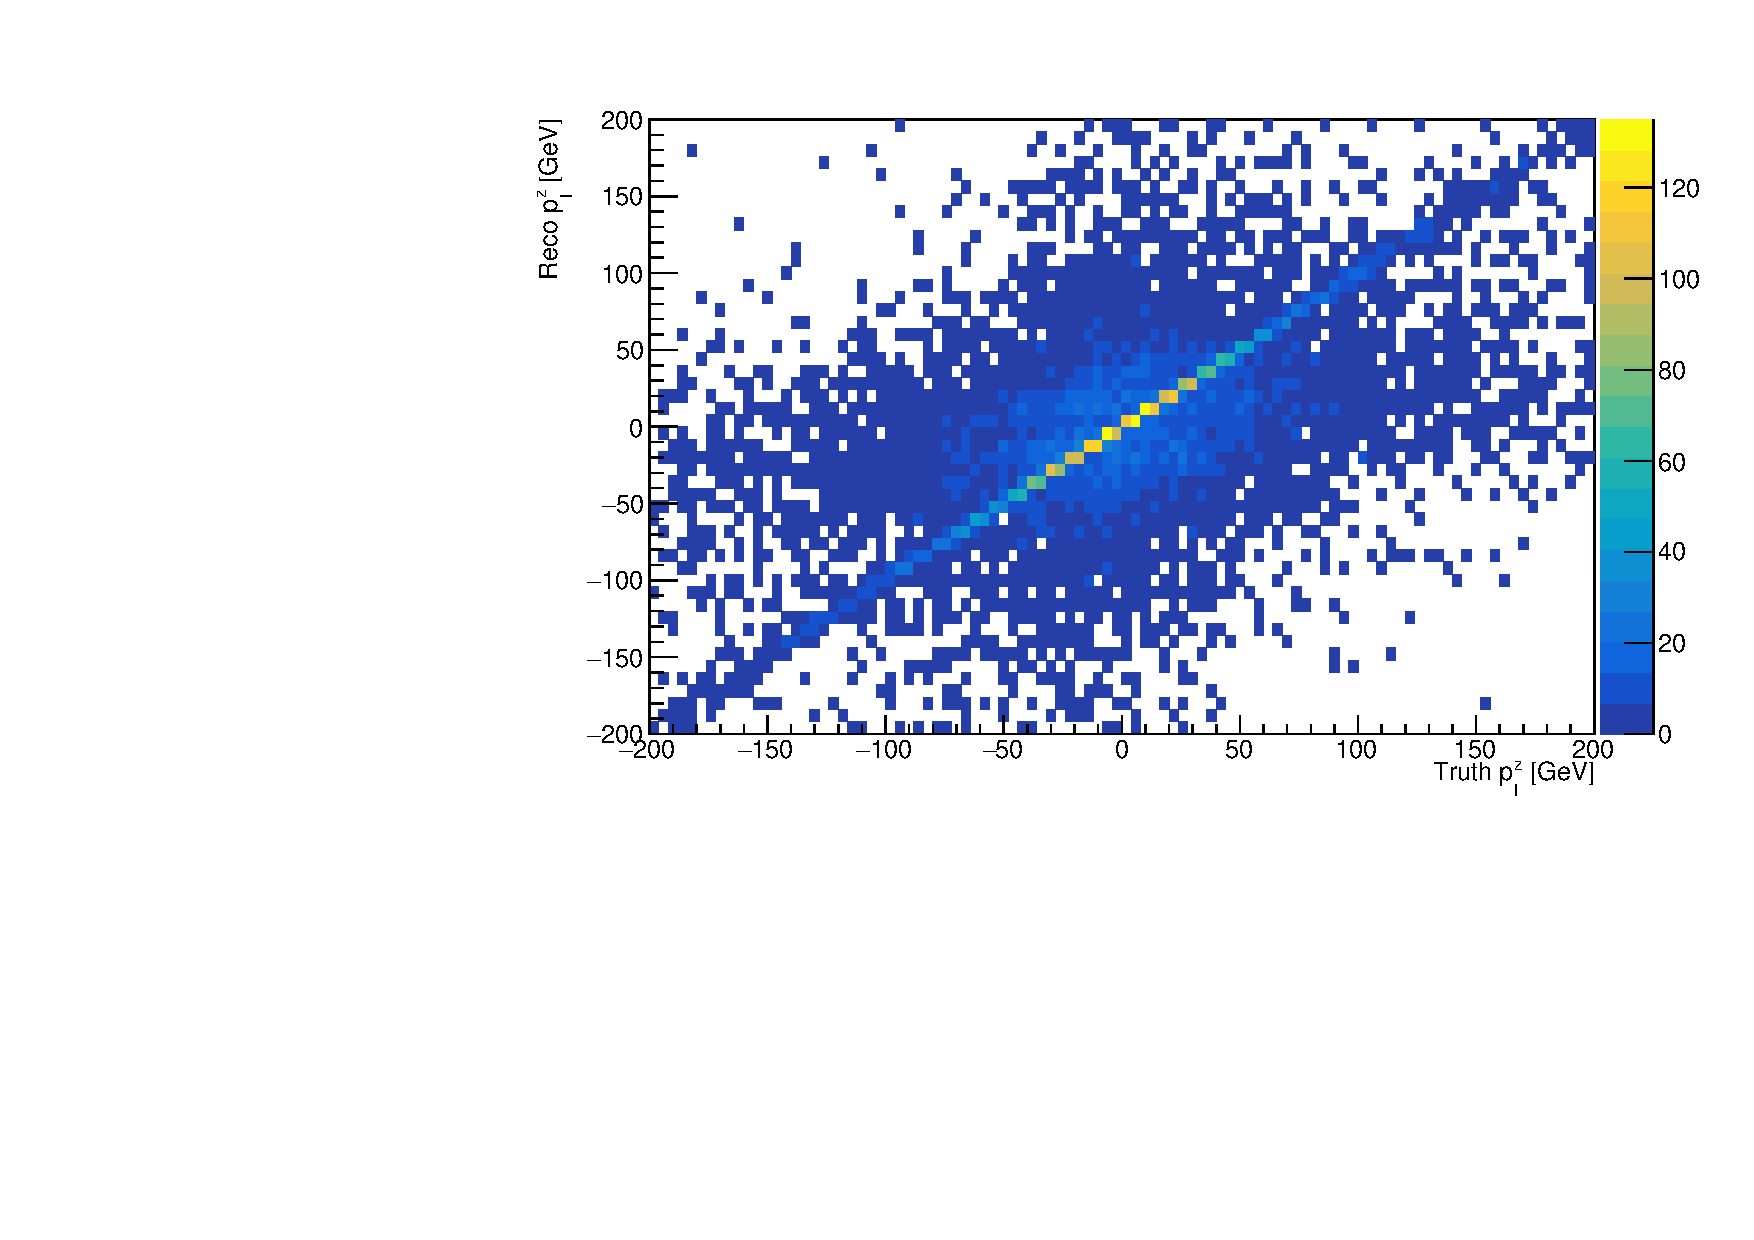
\includegraphics[width=\linewidth]{Chapter5_tHq/Reconstruction/truth_vs_reco_pz_l_alp05}
	\caption{Reco. $p_{z}(\elll_{\text{top}})$ vs. Truth $p_{z}(\ell)$}
	\label{fig:tHq:EventReconstruction:TopSystem:hypothesis1:C}
	\end{subfigure}
\hfill 
	\begin{subfigure}{0.45\textwidth}
	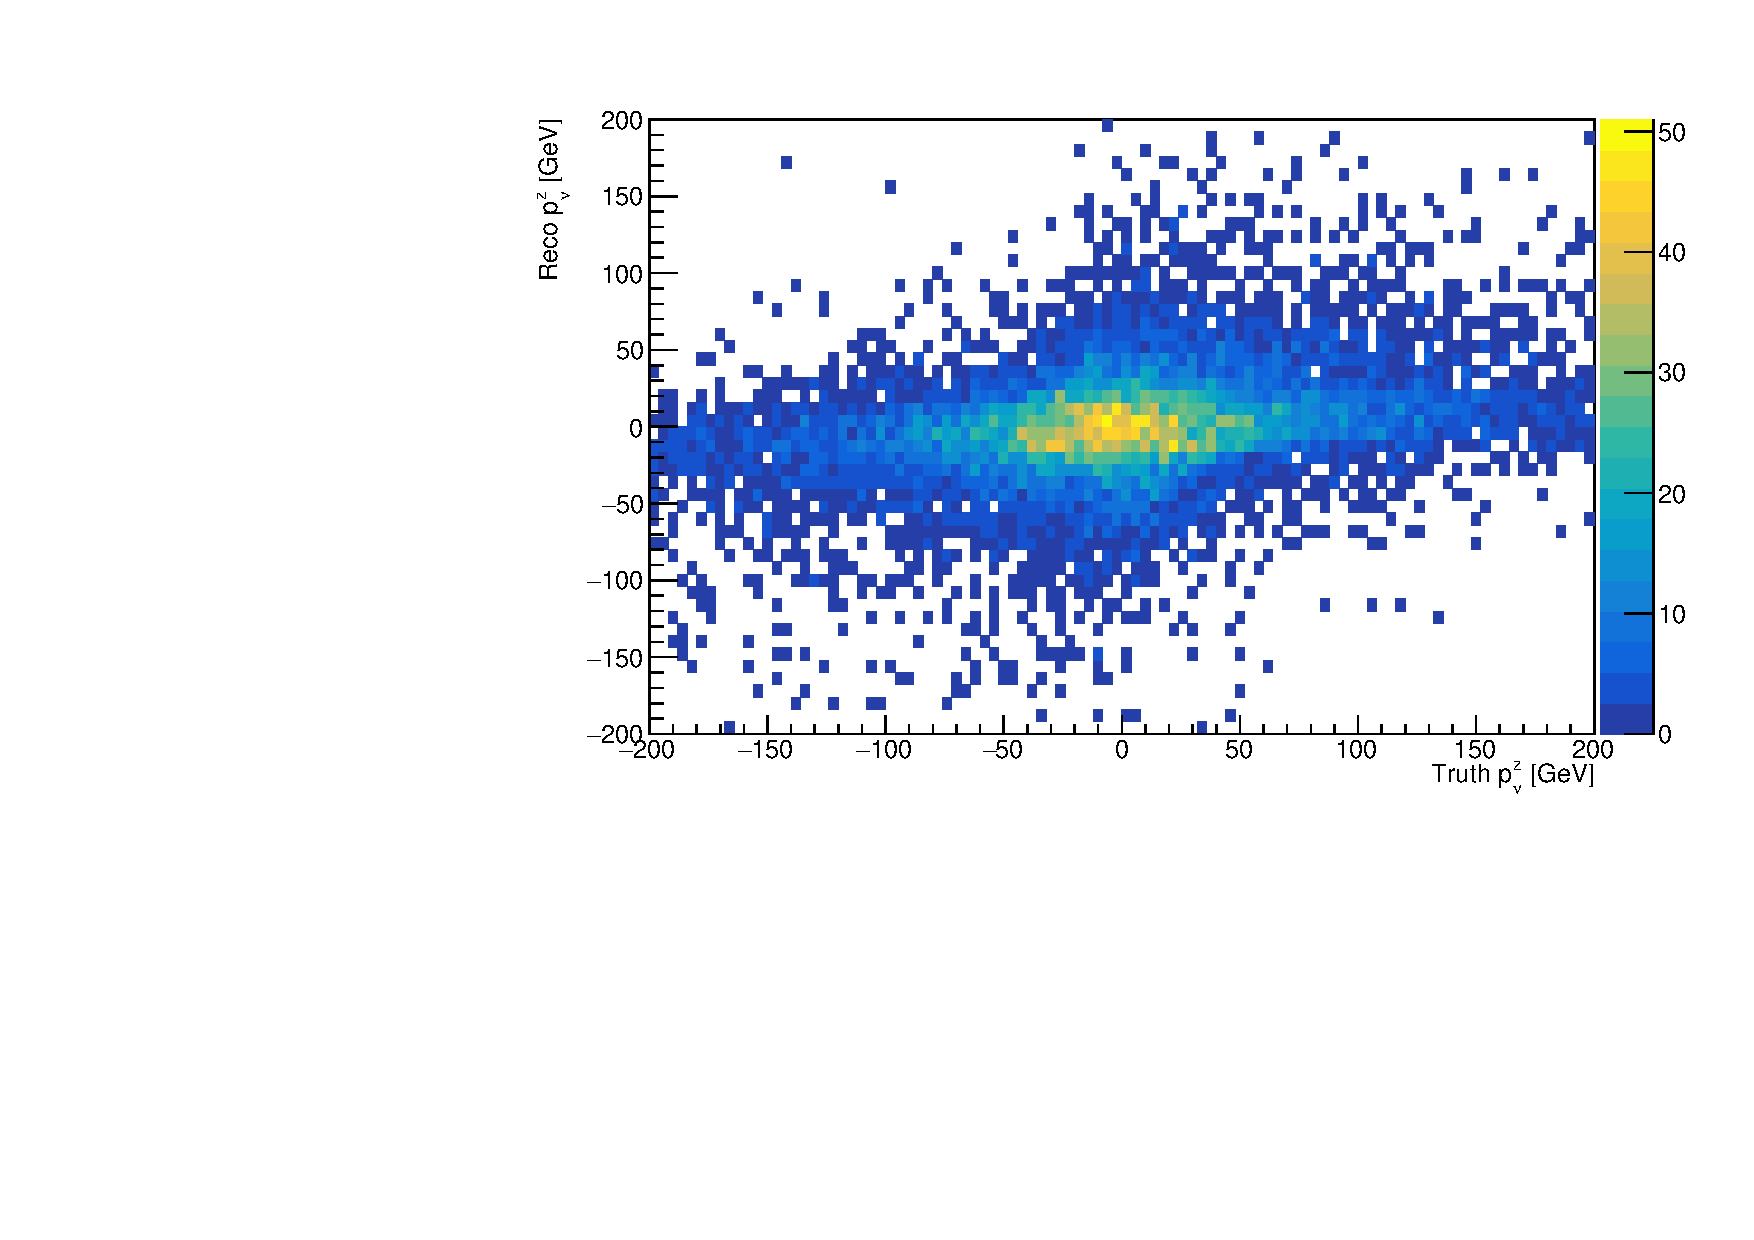
\includegraphics[width=\linewidth]{Chapter5_tHq/Reconstruction/truth_vs_reco_pz_nu_alp05}
	\caption{Reconstructed \pnutopz vs Truth \pnutopz}
	\label{fig:tHq:EventReconstruction:TopSystem:hypothesis1:D}
	\end{subfigure}

\caption{Distributions comparing \pnutopz and $p_{z}(\ell_{\text{top}})$
at truth and reconstruction levels for \tHq \dileptau events.} % Overall figure caption
\label{fig:tHq:EventReconstruction:TopSystem:hypothesis1}
\end{figure}
\end{comment}


Regarding the $\overrightarrow{E}_{\text{T}}^{\text{miss}}$ of the top-quark system, 
%In order to reconstruct the kinematics of the top quark, 
constraints have to be 
imposed on the $\Pnu_{\text{top}}$. Through the correlation analysis between the neutrino and 
the top-quark lepton, the following constraints were found in a linear fit:
\begin{align*}
    \pnutopT & =\frac{1615.98\, \text{GeV}^2}{\pltopT}\,,\\
    \phinutop &= \philtop\pm\frac{\pi}{2}\, ,
\end{align*}
where \phinutop and \philtop are, the azimuthal angles of the 
the neutrino and the reconstructed $\ell_{\text{top}}$, respectively, and 
\pnutopT and \pltopT their transverse momentums. The behaviour represented
by these constraints can be observed in Figure~\ref{fig:tHq:EventReconstruction:TopSystem:Reco}.

To resolve the sign ambiguity in the $\pm$ of the second constraint, the azimuthal 
angle of the \Pbottom quark originated on the top-quark decay (\phibtop) considered. 
The following condition is imposed:
\begin{align*}
  \phibtop-\philtop \geq 0 & \rightarrow \phinutop=\philtop-\frac{\pi}{2}\,,\\
  \phibtop-\philtop < 0  & \rightarrow \phinutop=\philtop+\frac{\pi}{2}\, .
\end{align*}


\begin{figure}[h] 
	\begin{subfigure}{0.49\textwidth}
	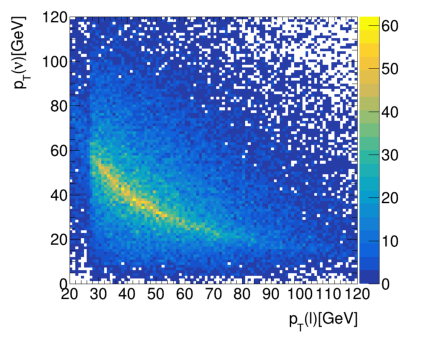
\includegraphics[width=\linewidth]{Chapter5_tHq/Reconstruction/topreco_pt}
	\caption{\pnutopT vs \pltopT}
	\label{fig:tHq:EventReconstruction:TopSystem:hypothesis2:pt}
	\end{subfigure}
\hfill 
	\begin{subfigure}{0.49\textwidth}
	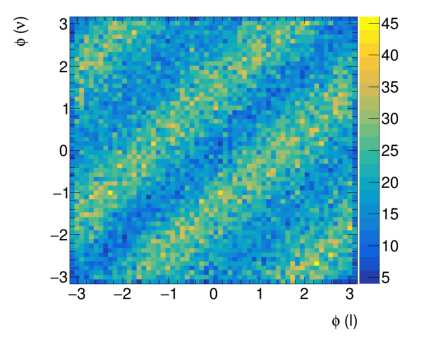
\includegraphics[width=\linewidth]{Chapter5_tHq/Reconstruction/topreco_phi}
	\caption{\phinutop vs \philtop}
	\label{fig:tHq:EventReconstruction:TopSystem:hypothesis2:phi}
	\end{subfigure}
\caption{Truth-level distributions comparing the $\pT$ (a) and $\phi$ (b) of the $\Pnu_{\text{top}}$ nd  $\ell{\text{top}}$.
With these two plots are obtained the imposted conditions at reconstruction level on \pnutopT and \phinutop.} 
\label{fig:tHq:EventReconstruction:TopSystem:Reco}
\end{figure}


The calculation of the reconstructed top-quark mass, \toprecomass, incorporates several 
variables, including the lepton associated with the top quark, the leading \bjet, and the 
neutrino \pnutopT and \phinutop. However, in this calculation, the \pnutopz
component is set to zero due to its unknown value.
With this it is possible to reconstruct the mass of the top quark and
to calculate $\pT^{miss}(\PHiggs)$. The latter is used in the reconstruction
of the Higgs boson. 

%%%%
%. Higgs boson reconstruction
%%%
\subsubsection{Reconstruction of the Higgs boson}
\label{sec:ChaptH:Sig:EventReconstruction:Higgs}
%The mass reconstruction plays a crucial role in creating discriminating variables. 
A straightforward method for reconstructing the Higgs-boson mass involves 
summing its visible decay products. Assuming the \Htautau decay mode:
\begin{equation*}
\Hvismass = \text{mass}(\Pgt_{\text{vis}, 1} + \Pgt_{\text{vis}, 2}) \, ,
\end{equation*}
where $\tauvis$ is either the visible part of the \tauhad
or the light lepton from the \taulep.

However, this approach overlooks the contribution of neutrinos and is therefore insufficient. 
By neglecting smaller contributions to the \MET, such as energy loss in detector material, 
it becomes possible to relate $\pT^{\text{miss}}(\PHiggs)$ to the measured \MET and the 
$\pT^{\text{miss}}(\Ptop)$ by imposing the relation:
\begin{equation*}
    p^{\text{miss}}_{x,y}(\PH) = p^{\text{miss}}_{x,y}(\text{measured})
      - p^{\text{miss}}_{x,y}(\text{top, reconstructed})\,.
\end{equation*}
This characteristic can be effectively employed in established methods for reconstructing 
the Higgs-boson mass.
The quantities \pnutopT and \phinutop, calculated in the previous section, are used in this relation.

There are several techniques to reconstruct the $\Ptauon\APtauon$ system. Among these,
the most popular methods are:
\begin{itemize}
	\item Partial invariant mass: Also known as \textit{Transverse Mass Method}, it uses
		the \Hvismass and the transverse mass of the $\Ptauon\APtauon$ system:
		\begin{equation*}
			m_{\text{T}}^{2} = m^{2} (\Ptau_{\text{vis}1}, \Ptau_{\text{vis}2}, \MET(\tau\text{-syst}) )\,.
		\end{equation*}
		This technique was first used in the UA1 experiment~\cite{Rubbia:155129} and has
		the advantage that it can be applied to all signal event topologies for the 
		$H \rightarrow \Ptauon \APtauon$ channel (i.e. $\tauhad \tauhad$, $\tauhad \taulep$ and $\taulep \taulep$). 
		The dedicated studies have show that the distributions of the reconstructed \mH using this method is
		lower than the one obtained with the parton-level \mH.
		
	\item Collinear approximation~\cite{Ellis:1987xu}: This is one of the most commonly 
		used techniques for the reconstruction of the invariant mass of a $\Ptau\APtauon$ 
		system with the presence of invisible decays products.
		It is mainly based on the assumption that $\Ptau$-lepton and all its decay
		products are collinear. In our search, these can be translated into having a boosted
		Higgs, which is not the case for the \tHq production.
		Another inconvenience of this method is that it is very sensitive to the
		resolution of \MET, being likely to overestimate the mass. 
		
	\item In the bibliography there are other mechanisms to solve this issue such as the 
		Recursive Jigsaw Reconstruction~\cite{Jackson:2017gcy} or the 
		Kinematic Likelihood Fitter~\cite{Erdmann:2013rxa}.
		
		
%source: https://www.overleaf.com/project/5f74653051c93a00018b5f95
\end{itemize}

A more sophisticated technique that outperforms the mentioned above is the \MMC (MMC), which was originally developed for the \Htautau analysis~\cite{ELAGIN2011481,ATLAS:2012gfw}. 
The MMC does not suffer from any of the limitations of the previous methods. It allows for a more complete reconstruction
of event kinematics with improved resolution for the mass of Higgs-boson-decay. 
This method is based on assuming that the source of $\MET(\PHiggs\text{-system})$ is 
due to the neutrinos from $\Ptau$ decays exclusively. Then, for each event, it scans over all possible
configurations of the visible and invisible \Ptau-decay products. 
It is based on the requirement that mutual orientations of the neutrinos and other decay products are consistent with the mass and decay kinematics of a \Ptau lepton. This is achieved by minimising a likelihood function defined in the kinematically allowed phase space region. 
Due to its better functioning, the MMC is the technique used in this analysis.


%%%%%%%%%%%%%%%%%%%
%           Background estimation        %
%%%%%%%%%%%%%%%%%%%
\section{Background estimation}
\label{sec:ChaptH:Bkg}
In our analysis, background events are classified into two distinct types:  
``reducible'' backgrounds and ``irreducible'' backgrounds.
\begin{itemize}
	\item \textbf{Irreducible backgrounds}: Irreducible backgrounds refer to processes whose 
		final states have the same physical objects as the signal.
		%These backgrounds cannot be distinguished from the signal based
		%on their properties alone. 
		The most important irreducible backgrounds in this 
		analysis are Diboson, \tW, \ttZ, \ttH, \ttW and \tZq.
		% The objects in the irreducible backgrounds are PROMPT objects.
	\item \textbf{Reducible backgrounds}:  The reducible backgrounds 
		are originated from inaccuracies in the reconstruction process. In other words,
		some objects are wrongly reconstructed as one of the objects that are present in the signal process.
		%For example, a high-energy electron can produce a signature that closely resembles 
		%that of  a high-energy photon. This can lead to identify this electron as it was photon,
		%constituting a misidentified photon.
		The misidentification of one or more objects can make non-signal process have
		the same final-state objects as that are present in the signal process. 
		If the experimental tools and techniques are improved, the effects of this type of background
		can be reduced.
		
		In the \dileptau channel, the dominant backgrounds consist of reducible events 
		where jets misidentified as \tauhad are present. This is particularly observed in 
		the \ttbar and \Zjets backgrounds. Additionally, other backgrounds include
		diboson (VV) and \ttX productions, such 
		as \ttH, \ttZ, and \ttW. Note that some background processes can belong to both categories.
		simultaneously.  
		
		%In the analysis presented in this thesis, the most relevant contribution to the background
		%comes from the misidentification of \tauhad, which leads to \ttbar, \PZ + jets backgrounds.
		% The objects in the reducible backgrounds are FAKE objects.
\end{itemize}

%As mentioned, the misidentification of \tauhad is the main source of background. 
In Section~\ref{sec:Chap3:Reco:Tau} it has been already noted that the task of rejecting 
quark- and gluon-originated jets for \tauhad reconstruction is challenging. 
Particularly, the difficulty in distinguishing hadronic taus 
from jets leads to a high rate of misidentification. %where jets are erroneously classified as 
%taus.  
But this is not the only type of reducible background that plays a role in the 
\tHq search in the \dileptau final state. The sources of reducible background are:
\begin{itemize}
	\item Gluon-initiated jet misidentified as \tauhad
	\item Quark-initiated misidentified as \tauhad
	\item Other object misidentified as \tauhad
	\item Misidentified or non-prompt light leptons\footnote{ Electrons and muons from meson decays and electrons from photon conversions. The heavy-flavour hadron decays produce a weak boson that decays to leptons.}
	\item Charge misidentification of leptons. 
\end{itemize}

Table~\ref{tab:ChaptH:BkgEst:Origins} provides a comprehensive overview of the estimated contribution of the different
sources of reducible backgrounds in the \dileptau channel. As can be seen, the misidentification of \tauhad is the most important
source of background in the \dilepOStau channel while for the \dilepSStau the fraction of misidentified particles is much smaller. 
%Additionally, a detailed split of these contributions by sample is presented in Figure~\ref{}, with exhaustive tables available in Appendix~\ref{}.

\begin{table}[h]
\centering
\begin{tabular}{lc|c}
\cline{2-3}
                   		& \multicolumn{2}{c}{Backgrounds} \\ \cline{2-3}
                   		& \dilepOStau      	& \dilepSStau  \\
				\midrule
\multicolumn{1}{l|}{Irreducible}        			&   $472\pm 6$ 	& $81.3 \pm 1.6$   		\\
\multicolumn{1}{l|}{Gluon identified as \tauhad}  	&   $1567\pm 27$ 	& $9.2 \pm 0.6$	   	\\
\multicolumn{1}{l|}{Quark identified as \tauhad} 	&   $5640\pm 70$ 	& $23.0 \pm 1.1$	   	\\
\multicolumn{1}{l|}{Other misidentified \tauhad} 	&   $2240\pm 50$ 	& $2.8 \pm 0.4$	   	\\
\multicolumn{1}{l|}{Misidentified \emu}          	&   $28.3\pm 1.9$ 	& $19.6 \pm 1.6$	   	\\
\multicolumn{1}{l|}{\Pe charge  flip}   	&   $340\pm 13$ 	& $33.0 \pm 3.2$	   	\\
\bottomrule
\end{tabular}
\caption{Origin of the backgrounds determined by the matching of events at truth and reconstruction levels.
The yields have been obtained at preselection level. 
Note that one event can fall in several categories simultaneously~\cite{ThesisTanja}.}
%\pablo{Yields form Tanjas thesis. Ask Oleh for the latest numbers.}}
\label{tab:ChaptH:BkgEst:Origins}
\end{table}


Knowing with accuracy the expected fraction of each background process is fundamental to 
obtaining quality results.
While for the irreducible backgrounds, the yields are estimated with accuracy in the MC-based simulations, 
for the reducible backgrounds it is not trivial to determine its 
abundance.  This is because the reducible backgrounds can strongly depend on the details of the physics simulation, 
including non-perturbative regions where the simulation would not be expected to be reliable~\cite{ATLAS:2022swp}.
They also depend on the modelling of the material composition and response of the detector.
% The computing resources required to simulate these processes with a sufficient sample size would be prohibitive.

%The strategy to estimate the abundance of reducible backgrounds involves matching reconstructed objects in simulated 
%datasets with the corresponding simulated-parton-level objects using $\dR$ cones, as well as the use of data-driven approaches.
%The proportion of events featuring jets mimicking leptons are depicted in Figure~\ref{fig:piecharts_dileptau_total_vs_tHq}. 


Among the approaches for the estimation of misidentification rates, the \textit{template fit method} stands out, 
especially for taking advantage of the high number of available MC samples. This data-driven strategy to estimate the 
abundance of the different reducible backgrounds involves matching reconstructed objects in simulated 
datasets with the corresponding simulated-parton-level objects using $\dR=0.2$ cones. By doing this, the 
templates for physical objects (\Pe, \Pmu, \tauhad, quark-initiated jet, gluon-initiated jet, and unknown) 
are created. A template is a group of particles with the same truth label. These templates are constructed
in two loops. The first loop finds the truth label of the reconstructed leptons and the second the does
the same for the jets\footnote{The ATLAS-specific tools used for this are \texttt{IFFTruthClassifier} and the \texttt{TauTruthMatchingTool}. 
The former is used for \emu and the latter for \tauhad.}. 
The composition at parton-level of the reconstructed objects is presented in Figure~\ref{fig:piecharts_dileptau_total_vs_tHq}. 
There it can be seen that while the objects in the \tHq process are typically well reconstructed, the reconstructed \tauhad 
from the backgrounds is not a true \Ptau in most cases. 

Once the templates are ready, it is necessary to find their normalisation factors.
The normalisation is done by fitting the templates to match the
data in background-enriched control regions specially dedicated to estimating the templates.

%The construction of MC templates for misidentified \emu use the \texttt{IFFTruthClassifier}
%and for the non-prompt \tauhad the \texttt{TauTruthMatchingTool}. The first tool
%electrons and muons based on their type and origin % and is described in Reference~\cite{IFFTruthClassifier}
%The second matches the reconstructed tau 
%objects to the visible 4-momentum of truth-level leptons and jets within an angular distance of $\dR=0.2$. 


\begin{figure}[h]
  \begin{subfigure}[b]{0.99\linewidth}
       \centering
       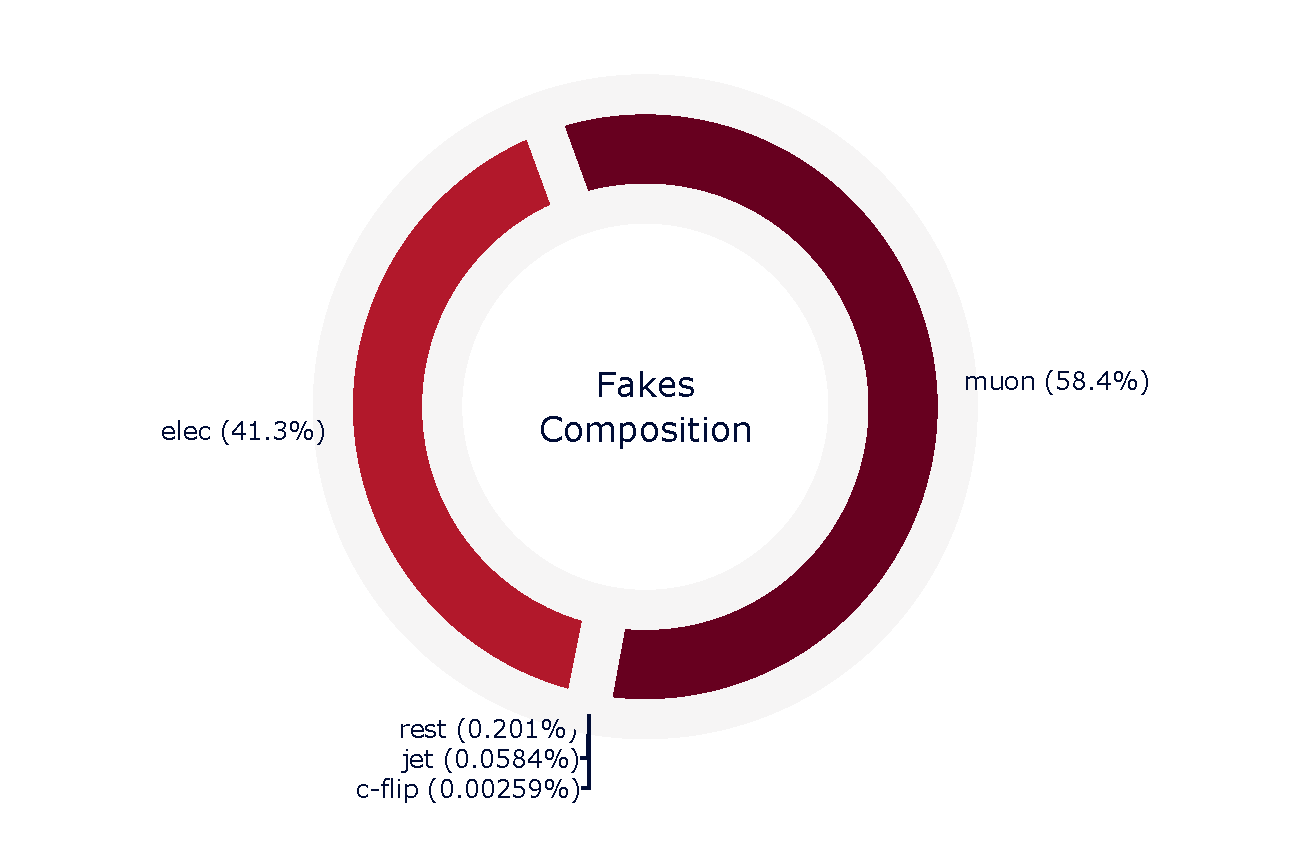
\includegraphics[width=0.30\linewidth]{Chapter5_tHq/fakes/SR_lep1tmp_lephad}
       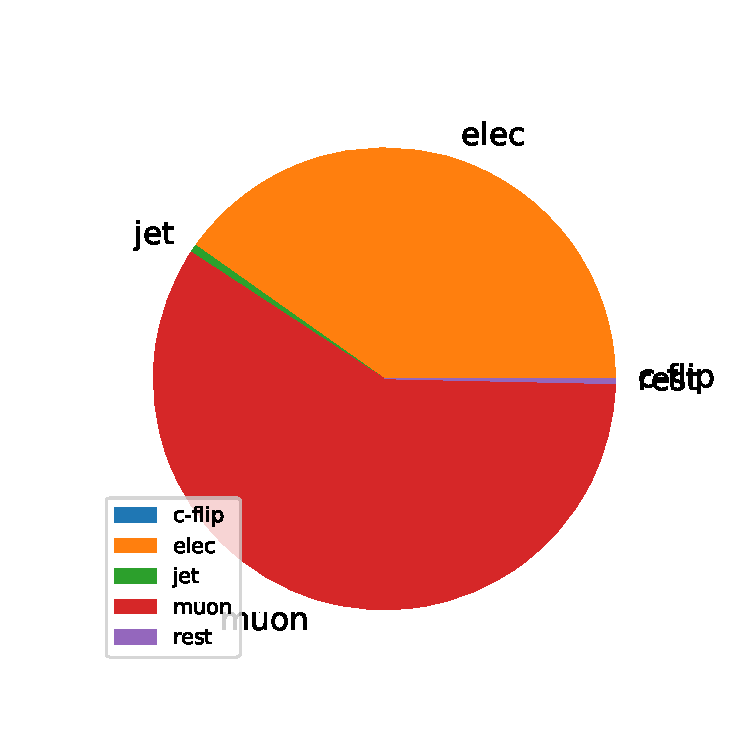
\includegraphics[width=0.30\linewidth]{Chapter5_tHq/fakes/SR_lep2tmp_lephad}
       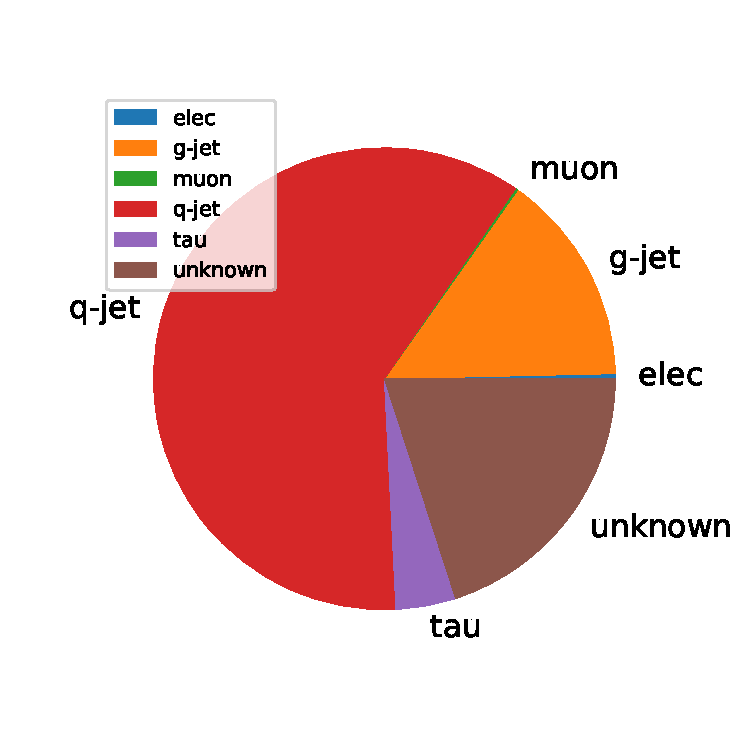
\includegraphics[width=0.30\linewidth]{Chapter5_tHq/fakes/SR_tau1tmp_lephad}
       \caption{Total MC}
  \end{subfigure}
  \begin{subfigure}[b]{0.99\linewidth}
      \centering
      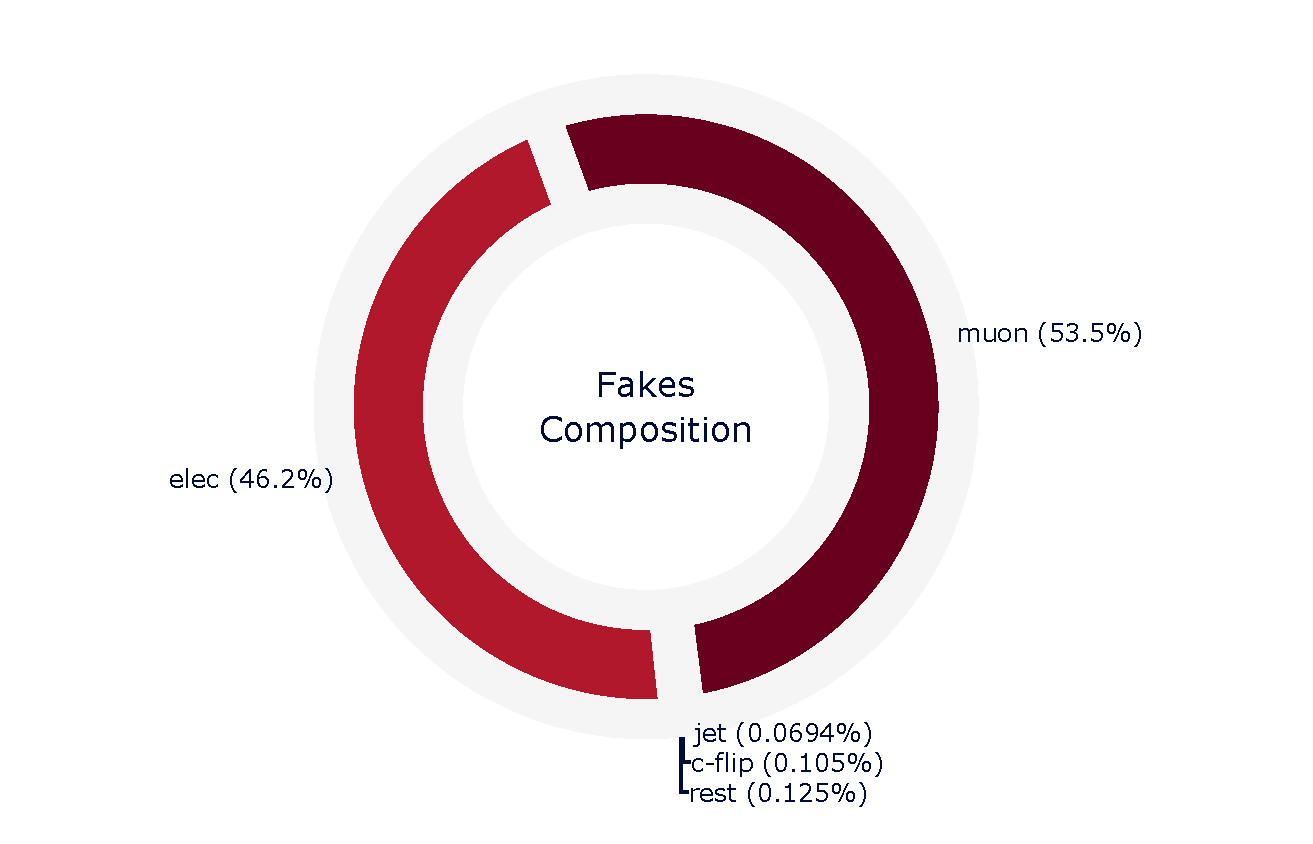
\includegraphics[width=0.30\linewidth]{Chapter5_tHq/fakes/SR_tH_lep1tmp_lephad}
      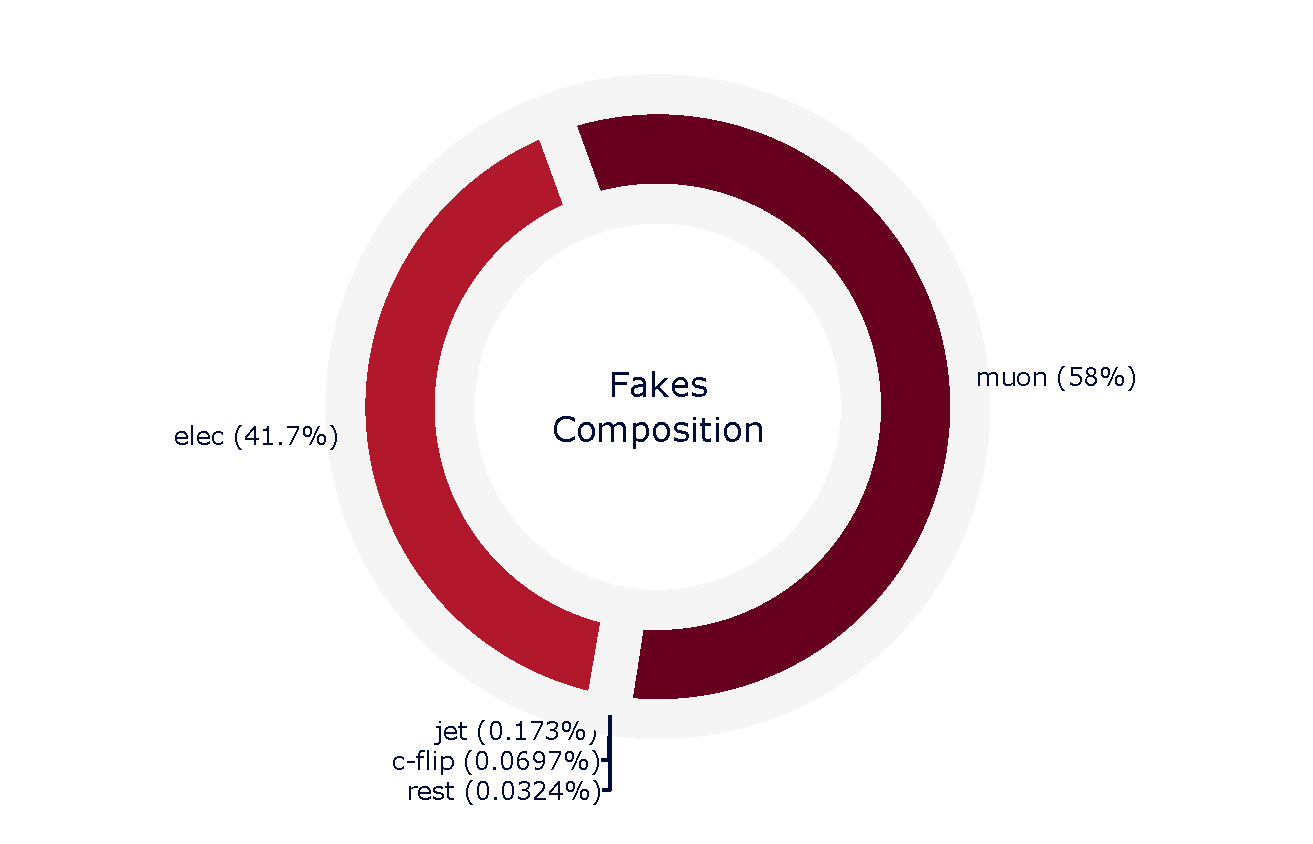
\includegraphics[width=0.30\linewidth]{Chapter5_tHq/fakes/SR_tH_lep2tmp_lephad}
      \includegraphics[width=0.30\linewidth]{Chapter5_tHq/fakes/SR_tH_tau1tmp_lephad}
      \caption{\tHq}
  \end{subfigure}
   \caption{Composition at parton level of the reconstructed leading (left) and sub-leading (middle) leptons, as well as \tauhad (right) passing the selection cuts in the \dileptau analysis with oppositely charged light leptons. The results are calculated using all MC samples and \tHq production.}
   \label{fig:piecharts_dileptau_total_vs_tHq}
\end{figure}




Then, the estimation of the misidentification-based background events and the assessment of the corresponding 
uncertainty are done separately for the \dilepOStau and \dilepSStau channels. For the \dilepOStau channel, the
estimation of the SFs is conducted as follows:

\begin{enumerate}
	\item To compensate for the potential mismodelling of quark- and gluon-initiated jets mimicking \tauhad, 
		the template fit of the quark and gluon components is performed in a region enriched with 
		misidentified-\tauhad. This region of the phase space is defined in a way that the \tauhad candidates
		do not pass the \texttt{medium} identification criteria (see Section~\ref{sec:ChaptH:ObjectDefReco:tau}
		for identification working points).
		%This region is defined by requiring that the light leptons fail their 
		%identification and isolation requirements described in 
		%Table~\ref{tab:ChaptH:ObjectDefReco:Electrons_Muons}. 
		The template fit is used here is the nominal method. It is assumed that the SFs derived this 
		way can be extrapolated to the rest
		of the analysis regions and, hence, these are applied to all MC samples.


	\item Secondly, the number of real and misidentified \tauhad candidates is counted in the same region
		%This misidentified-\tauhad-enriched region, is used to determine the correction factor
		%that aligns the MC to the data. 
		With these counts, the correction factors
		that align the MC to the data are derived
		This is known as the \textit{counting method} and it is the alternative approach
		used to assess the uncertainty of the nominal method.
		In the counting method, the SFs are derived separately for:  
		\begin{itemize}
			\item 1-prong and 3-prong \tauhad decays. 
			\item  Various \pT(\tauhad) bins.
			\item  1 and 2 \bjets multiplicity.
		\end{itemize}
		Therefore, different SFs are derived for different regions of the phase space. 
		No significant dependence on $|\eta(\tauhad)|$ is observed.
		
		
	\item Finally, using the samples with adjusted misidentified-\tauhad rates, the estimation of the 
		misinterpretation rates for light leptons is calculated. Similarly to the \tauhad case,
		the correction factors to be applied to MC are determined to match the templates to the data in a 
		misidentified-$\ell$-enriched region.
		This region is defined by requiring that the light leptons fail their 
		identification and isolation requirements described in 
		Table~\ref{tab:ChaptH:ObjectDefReco:Electrons_Muons}
		 A simplified classification scheme is used to construct the templates
		for the leptons.
\end{enumerate}



%%%%
% Same Sign fake rates
%%%%
Meanwhile, for the \dilepSStau channel, the condition on the electric charge of the
light leptons produces a drastic decrease in the influence of the \tauhad-misidentification rates.
This is shown in Figure~\ref{fig:piecharts_dileptau_SS_total_vs_tHq}, which is the same
as Figure~\ref{fig:piecharts_dileptau_total_vs_tHq} but only with \dilepSStau events.

Due to the limitation of the statistical sample, the techniques applied for the estimation of the backgrounds 
arising from misidentified objects in the \dilepSStau channel are
a simplified version of those used in the \dilepOStau.
The simplification consists of using just a single template combining the quark- and gluon-initiated jets, and
not splitting the sample by the number of \btagged jets. 

 
%Data-driven methods are used to adjust the simulated event rates for backgrounds originated from jets that 
%are misidentified as taus and light leptons.
% The electron charge is determined with a BDT and to minimise the background presence of misidentified electron charge, an additional cut is imposed on the BDT for charge identification score (ECIDS). 


\begin{figure}[h]
  \begin{subfigure}[b]{0.99\linewidth}
       \centering
       \includegraphics[width=0.30\linewidth]{Chapter5_tHq/fakes/SS_SR_lep1tmp_lephad}
       \includegraphics[width=0.30\linewidth]{Chapter5_tHq/fakes/SS_SR_lep2tmp_lephad}
       \includegraphics[width=0.30\linewidth]{Chapter5_tHq/fakes/SS_SR_tau1tmp_lephad}
       \caption{Total MC}
       \label{fig:piecharts_dileptau_SS_total_vs_tHq:tot}
  \end{subfigure}
  \begin{subfigure}[b]{0.99\linewidth}
      \centering
      \includegraphics[width=0.30\linewidth]{Chapter5_tHq/fakes/SS_SR_tH_lep1tmp_lephad}
      \includegraphics[width=0.30\linewidth]{Chapter5_tHq/fakes/SS_SR_tH_lep2tmp_lephad}
      \includegraphics[width=0.30\linewidth]{Chapter5_tHq/fakes/SS_SR_tH_tau1tmp_lephad}
      \caption{\tHq}
      \label{fig:piecharts_dileptau_SS_total_vs_tHq:tHq}
  \end{subfigure}
   \caption{Composition at parton level of the reconstructed leading (\textit{left}) and sub-leading (\textit{middle}) leptons, as well as
   \tauhad (\textit{right}) in the \dilepSStau analysis channel. The numbers are computed for the combined
   MC samples (\textit{a}) and \tHq production only (\textit{b}). An electron charge ID selector has been applied to this data.
   Note that while the pie charts distinguish between quark- and gluon-initiated jets, these two processes use a single 
   template in the template fit method for the \dilepSStau channel.}
   \label{fig:piecharts_dileptau_SS_total_vs_tHq}
\end{figure}

As Figure~\ref{fig:piecharts_dileptau_SS_total_vs_tHq} shows, while the fraction of correctly identified \tauhad improves in the \dilepSStau,
the influence of jets being misinterpreted as leptons is considerable for the
sub-leading leptons (see the green section in the second pie chart of 
Figure~\ref{fig:piecharts_dileptau_SS_total_vs_tHq:tot}).
To minimise the background arising from incorrect identification of the electron charge, an electron 
charge identification selector (ECIDS) is implemented in the \dilepSStau channel~\cite{ATLAS:2019qmc}.



%Alternatively, to derive the normalisation of misidentified \tauhad, the counting method can be used.
%In a region with high density of misidentified \tauhad, if the simulated fake rate agrees with the data in that 
%region, it is assumed to be reliable in the rest of the regions of the analysis region.
%If the MC is not matching the data, a correction factor is applied and this same factor
%is derived through the rest of the regions.

%By doing this, normalisation factors (referred to as misidentification scale factors) are derived 
%for each process and for different regions of the phase space defined by $\pT$, multiplicity
%of \btagged jets (one or two), and the number of prongs (one or three).  No dependence 
%on $|\eta|$ was found.



%\paragraph{Tau fakes}
%In the analysis channels involving hadronic taus, all methods used for fake background estimation rely
%on MC-based templates. These are splits of simulation according to a type of object mimicking the
%lepton of interest. Construction of MC templates related to the electron and muon fakes is based on
%\texttt{TruthClassificationTool} tool.
%\pablo{Describe the \texttt{TruthClassificationTool}}
%\begin{itemize}
%	\item counting method
%	\item template fit method
%\end{itemize}
%The extracted SFs are then applied to the simulated background component
%in the region with taus passing the preselection requirements.

%%%%%%%%%%%%%%%%
%     Reducible backgrounds  %
%%%%%%%%%%%%%%%%
%\subsection{Reducible backgrounds}
%\label{sec:ChaptH:Bkg:Fakes}
%\pablo{"Tools for estimating fake/non-prompt lepton bkgs" in reference~\cite{ATLAS:2022swp}}

%\pablo{Añadir en esta sección la información de este paper:
%\url{https://arxiv.org/pdf/2211.16178.pdf}. "Tools for estimating fake/non-prompt lepton
%backgrounds with the ATLAS detector at the LHC"}


%\paragraph{Light-lepton fakes} % When talking about promt, non-prompt and fakes it is recomended to avoid the work real.
%Particles from the hard scattering process are referred to as `prompt'. 
%Acceptance, quality and isolation requirements are applied to select these leptons
%Non-prompt leptons and non-leptonic particles may satisfy these selection criteria, 
%giving rise to so called `non-prompt and fake' lepton backgrounds.
%Fake electrons/muons will not be explicitly distinguished and are referred to as fake leptons.
%The mis-identified lepton background arises from leptons from heavy-flavour 
%($\Pl_{\text{HF}}$) hadron decay and electrons from \Pgamma-conversions.
%These leptons are mainly produced in \ttbar, \Zjets and tW events.

%The estimation of the fake/non-prompt lepton background is done with the template fit method or via the matrix method

%The fake and real lepton efficiencies (fake/real rates) are defined as the probabilities of a fake or real
%electron or muon to pass the nominal electron/muon requirements. They are given by the tight over loose ratio

%Get some ideas from here: \url{https://cds.cern.ch/record/1951336/files/ATLAS-CONF-2014-058.pdf}

%\paragraph{Tau fakes}
%In the analysis channels involving hadronic taus, all methods used for fake background estimation rely
%on MC-based templates. These are splits of simulation according to a type of object mimicking the
%lepton of interest. Construction of MC templates related to the electron and muon fakes is based on
%\texttt{TruthClassificationTool} tool.
%\pablo{Describe the \texttt{TruthClassificationTool}}
%\begin{itemize}
%	\item counting method
%	\item template fit method
%\end{itemize}
%The extracted SFs are then applied to the simulated background component
%in the region with taus passing the preselection requirements.
%Reducible backgrounds: \ttbar, \PZ + jets 


%%%%%%%%%%%%%%%%
%     Irreducible backgrounds   %
%%%%%%%%%%%%%%%%
%\subsection{Irreducible backgrounds}
%\label{sec:ChaptH:Bkg:Irreducible}
%All the processes whose signature is the same as the process of interest are known as irreducible backgrounds as in
%contrast to the fake or reducible backgrounds described in Section~\ref{sec:ChaptH:Bkg:Fakes}. The objects in 
%the irreducible backgrounds are prompt. The main irreducible backgrounds are:
%Irreducible backgrounds: Diboson, \tW, \ttZ, \ttH,\ttW, \tZq,



%%%%%%%%%%%%%%%%%%
%             Event selection              %
%%%%%%%%%%%%%%%%%%
\section{Event selection}
\label{sec:ChaptH:EventSelection}
%The event selection consists on the application of a set of conditions
%that allow us to separate the signal from the background.
The event selection consists of enriching the relative contribution of the
signal over background. %in a region of the phase-space. 
By doing so, we define a region of the phase space 
that is enriched with signal events. This region is called 
signal region (SR).

%Signal (aka needle). -> Several needels
%Background (aka haystack) -> Several types of haystacks

The signal selection is performed in several steps and using different methods. First of all, we define a 
preselection region (PR), where the physical objects are selected according to the detector acceptance.
The PR is described in Section~\ref{sec:ChaptH:EventSelection:PR}.
%The PR is a cut-based region and it is described in Section~\ref{sec:ChaptH:EventSelection:PR} . 
Then, discriminant variables are defined and used as input features for a BDT that  
can distinguish between signal-like and background-like events by creating a discriminant 
known as ``BDT score''. 
% \footnote{Actually it separates a target process from the others. More details about the BDTs
% can be found in Appendix~\ref{chap:Appendix:BDT}.}
The training of the BDTs for the region definition is discussed in 
Section~\ref{sec:ChaptH:EventSelection:BDT}.
Finally, by applying requirements on the BDT outputs, the SR is 
defined (see Section~\ref{sec:ChaptH:EventSelection:SR}).
 Additional regions dedicated to background processes
can also be defined (see Section~\ref{sec:ChaptH:EventSelection:CR}). 
The regions of the phase space enriched with
particular background processes are referred to as control (CR)
or validation regions (VR). 
The difference between CR and VR is that while the former
are considered into the fit calculations (discussed in Section~\ref{sec:ChaptH:Fit}), the latter are not.
The SR, CRs and VRs are all orthogonal and are subspaces of the PR.



Two figures of merit are used to optimise both the fraction of signal events in the data and the
absolute number of signal events. These metrics are the \StoB or purity and the signal significance,
respectively:
\begin{itemize}
\item \textbf{Purity}: 	The purity of a process is defined as the ratio between the 
				event yields of the target process and the total yields. For the signal process, 
				instead of purity, the signal to background ratio (\StoB) is used.
				
\item \textbf{Significance}:	This metric does not only account for the relative fraction of the
					process of interest but also the total amount of events. Using
					the significance as metric enhances the importance of keeping 
					enough statistics. 
					
					The definition of the significance estimator used in this work is
					the one given in Reference~\cite{Cowan:2010js}: % Cowan eq. (96)
					% http://www.phys.ufl.edu/~korytov/phz6355/note_A13_statistics.pdf <- Formula from here
					% https://indico.cern.ch/event/287744/contributions/1641250/attachments/535751/738667/Verkerke_Statistics_1.pdf <-  Formula also appears here
					% 
					\begin{equation*}
						\text{Significance} = \sqrt{2 [(s+b) \text{ln}(1+s/b) - s]} \approx \frac{s}{\sqrt{s+b}},
					\end{equation*}
					where $s$ is the number of events of the target process 
					and $b$ is the number of yields for the rest of processes 
					combined. This can be used not only to evaluate the signal 
					significance but also the significance of the background proceses
					in the dedicated background-enriched regions.
\end{itemize}
			
%%%%%%%%
%     Preselection
%%%%%%%%
\subsection{Preselection}
\label{sec:ChaptH:EventSelection:PR}
The starting point on the region definition is a collection of events 
that are reconstructed as \tHq events and with objects that
pass the reconstruction requirements defined in Section~\ref{sec:ChaptH:ObjectDefReco}.
These events
are produced by SingleTopAnalysis from AnalysisTop in combination with the
\thqloop framework, as it is described in Section~\ref{sec:ChaptH:Data_and_MC}.

Firstly, preselection requirements are applied to guarantee the orthogonality between the 
different \tHq channels. These requirements are the obvious ones in terms of number 
of final-state light leptons and hadronically decaying taus and are exclusive of the \dileptau channel.
\begin{itemize}
	\item One hadronically-decaying tau: $n(\tauhad)=1$.
	\item Two light-flavoured-charged leptons:  $n(\Pe / \Pmu)=2$.
\end{itemize}

The multiplicity of jets is constrained as well. From the Feynman diagrams 
in Figure~\ref{fig:tHq:intro:diltauFeynmanDiagram} it
can be seen that one non-\btagged jet and one \btagged jet can be expected. 
Although there are two \Pbottom-type quarks in the Feynman diagram,
the second\footnote{This quark is usually referred to as second \Pbottom in contrast to
the first, which is the one from the top quark decay.} 
\Pbottom-quark frequently goes undetected because its
\pT distribution is peaking around 2 or 3~GeV 
(see Figure~\ref{fig:tHq:pTvsEta_bQuark}) and, hence, it does
not pass the \pT threshold of the detector. 
For this reason, when only one jet is \btagged, 
it is assumed to either be the \Pbottom from the top-quark decay or a jet from secondary radiations.
These choices are motivated by maximising the signal acceptance while minimising the background contamination.

\begin{figure}[h]
\centering
\includegraphics[width=.49\textwidth]{Chapter5_tHq/Truth_b_quark_Comb_Stack_inverted}
\includegraphics[width=.49\textwidth]{Chapter5_tHq/Truth_b_quark_Comb_Stack}

\caption{Truth-level $\pT$ vs $\eta$ distributions for the spectator (or second) \Pbottom quark and 
the \Pbottom quark produced in the top quark decay for the \tHq events.
Note that in most cases the second \Pbottom quark is produced with very low \pT and, consequently, it does not pass the 
lepton-trigger requirements and, hence, it is not detected at ATLAS. This argumentation is used
to justify the  $\pT$ requirement on the \bjets.}
\label{fig:tHq:pTvsEta_bQuark}
\end{figure}

\begin{itemize}
	\item In total from two to six jets are requested. In the distribution of jets within the \tHq sample 
	(see Figure~\ref{fig:ChaptH::EventSelection:PRJetMultiplicity})
	can be observed that, as expected, the number of \tHq events drop at higher jet multiplicity: $n(\text{jet})=[2,\,6]$.
	This broad range in jet multiplicity is chosen strategically, as it will later be  incorporated
	in the training of the BDTs.
	\item From which exactly one or two are \btagged jets: $n(\bjet)=[1,\,2]$.
	\item For its detection and identification, the jets are required to be in $|\eta(\text{jet})|<4.5$ with $\pT(\text{jet})>20$~GeV
	\item For \btagged jets the pseudorapidity requirement is tighter $|\eta(\bjet)|<2.5$ because that is the
	coverage of the ID, which is necessary for \btag.
\end{itemize}

% m_n_jets
\begin{figure}[h]
\centering
\includegraphics[width=.75\textwidth]{Chapter5_tHq/Preselection_NormalisedDistribution_JetMultiplicity}
\caption{Normalised distribution of the jet multiplicity for all \tHq channels before applying any requirement.}
\label{fig:ChaptH::EventSelection:PRJetMultiplicity}
\end{figure}


\begin{comment}
% pt vs eta for t-channel
\begin{figure}
\centering
\begin{subfigure}{.5\textwidth}
  \centering
  \includegraphics[width=.9\linewidth]{Chapter1/single_top_pTvsEta_bquark}
  \caption{Bottom quark from the top-quark decay.}
  \label{fig:Chap1:top:singletop:tchannel:ptVSeta:b}
\end{subfigure}%
\begin{subfigure}{.5\textwidth}
  \centering
  \includegraphics[width=.9\linewidth]{Chapter1/single_top_pTvsEta_SECOND_bquark}
  \caption{Second bottom-quark.}
  \label{fig:Chap1:top:singletop:tchannel:ptVSeta:second_B}
\end{subfigure}
\caption{Truth-level kinematic $\pT$ vs $\eta$ distributions for the two \Pbottom quarks 
in the single top-quark \tchannel process.
In (a) the \Pbottom quark originated from the decay of the top quark. In (b) the second \Pbottom quark, 
which is the one arising from a gluon splitting into a \bbar pair. The simulated events were requirements 
produced within the 4FS using \PROTOS LO generator~\cite{ATLAS:2017rcx}. As can be seen, 
in most of cases the second \Pbottom quark is produced with vey low \pT and, consequently, it does not pass the 
lepton-trigger requirements and, hence, it is not detected at ATLAS. A similar distribution for the \tHq process is presented
in Figure~\ref{fig:tHq:pTvsEta_bQuark}.}
\label{fig:Chap1:top:singletop:tchannel:ptVSeta}
\end{figure}
\end{comment}

The preselection conditions also account for the geometrical acceptance of the 
detector and the trigger thresholds presented in Section~\ref{sec:Chap2:ATLAS}.
\begin{itemize}
	\item The reconstructed electrons must satisfy $|\eta(\Pe)|<2.47$ but $|\eta(\Pe)| \notin [1.37,\, 1.52]$ because
	we are vetoing the electrons in the crack region.  The $|\eta|<2.47$ corresponds to the acceptance of the electron
	clusters in the ECAL, as presented in Section~\ref{sec:Chap3:Reco:ElectronsAndPhotons}. In general, for \pT below 10~GeV it is not
	possible to reconstruct the electrons efficiently.
	% 10 GeV es la mínima energía de los electrones que se pueden reconstruir y calibrar bien el ID 
	% por debajo el pile-up lo estropea todo y las eficiencias se degradan. 
	% Cuanto más pT tiene un objeto mejor reconstruido/identificado (i.e. menos uncertainty).
	% bueno, hasta un cierto valor de pT (más que nada por la estadística, que te quedas sin ella)
	% hay que encontrar un compromiso entre tu aceptancia (i.e. que tengas suficientes eventos) 
	% y que los objetos estén bien definidos.
	% y tengan una unc. de ID y reco buena
	%.                                                                                    - Carlos
	We require $\pT(\Pe)$ to be larger than $14$~GeV to reject the low-\pT background from the pile-up.
	\item The muons have to be reconstructed within $|\eta(\Pmu)|<2.50$, which corresponds to the MS coverage.
	and must have a minimum transverse momentum of $\pT(\Pmu)>14$~GeV.
	\item The tau leptons are also vetoed in the crack region of the detector so $|\eta(\tauhad)|<2.50$ but 
	$|\eta(\tauhad)| \notin [1.37, 1.52]$ and to have at least $\pT(\tauhad)>20$~GeV.
\end{itemize}
The higher is the \pT of an object, the more efficient is its reconstruction. Therefore,
setting the \pT requirements at the PR aims to balance between achieving
good reconstruction quality and ensuring a sufficient amount of data (statistics) for analysis.

Other constraints are also applied
\begin{itemize}
	\item To remove the low-\MET backgrounds, we impose that a minimum \MET of 5~GeV.
	By demanding a maximum \MET of 800~GeV only one event is lost. By doing this, the BDTs can
	later use the entire \MET distribution to perform cuts. 
	The impact \MET requirements can be see on Figure~\ref{fig:ChaptH::EventSelection:MetCondition}.
	\item The two leading charged-leptons, ordered by \pT are required to have $\pT(\Plepton_{1})>27$~GeV
	and $\pT(\Plepton_{2})>20$~GeV.
	Note that this condition is not applied for the light-leptons but for the tau leptons as well.
	\item The sum of the charge of the leptons must be $\pm1$.
\end{itemize}

\begin{figure}[h]
\centering
\begin{subfigure}{.48\textwidth}
  \centering
  \includegraphics[width=.95\linewidth]{Chapter5_tHq/Preselection_MET_cut_PR_lower}
  \caption{Lower \MET cut.}
  %\label{}
\end{subfigure}%
\begin{subfigure}{.52 \textwidth}
  \centering
  \includegraphics[width=.95\linewidth]{Chapter5_tHq/Preselection_MET_cut_PR_upper}
  \caption{Upper \MET cut.}
  %\label{}
\end{subfigure}
\caption{Distributions to study the lower (a) and upper (b) requirements on the \MET~\cite{ThesisTanja}.
The \textit{All} in (a) refers to the events before applying any other PR condition.
All lepton-related requirements as well as the requirements on the total number of jets are applied. 
The evolution of the events for the \tHq, \ttbar and \Zjets samples depending on the lower \MET condition 
is presented in (a). There, all samples are reweighted to one event in the first bin.}
\label{fig:ChaptH::EventSelection:MetCondition}
\end{figure}


A summary of the preselection requisites is presented in
Table~\ref{tab:ChaptH:Preselection} and the effect of such conditions
can be observed in Figure~\ref{fig:ChaptH::EventSelection:PR_Cutflow}. 
The events that pass the preselection requirements
conform the  PR and the yields at this level are presented in Table~\ref{tab:ChaptH:EventSelection:Preselection}
Using the events in the PR, the BDTs presented
in Section~\ref{sec:ChaptH:EventSelection:BDT} are trained to define the SR and CR, 
as it is described in Sections~\ref{sec:ChaptH:EventSelection:SR} and \ref{sec:ChaptH:EventSelection:CR}, respectively. 


\begin{table}[h]
\begin{adjustbox}{max width=0.99\textwidth}
\begin{tabular}{llll}
\toprule
Object                         & Multiplicity               & Momentum                      & Pseudoroapidy                                                    \\  \midrule
\multirow{2}{*}{Light leptons} & \multirow{2}{*}{$n(\Pe / \Pmu)=2$} & $\pT(\Pe)>14\,$GeV            & $|\eta(\Pe)|<2.47$,\, $|\eta(\Pe)| \notin [1.37,\, 1.52]$         \\
                               &                                    & $\pT(\Pmu)>14\,$GeV           & $|\eta(\Pmu)|<2.50$                                              \\
Hadronic tau             & $n(\tauhad)=1$        & $\pT(\tauhad)>20\,$GeV        & $|\eta(\tauhad)|<2.50$,\, $|\eta(\tauhad)| \notin [1.37, 1.52]$ \\
Jets                           & $n(\text{jet})=[2,\,6]$    & $\pT(\text{jet})>20\,$GeV      & $|\eta(\text{jet})|<4.5$                                               \\
\btagged jets             & $n(\bjet)=[1,\,2]$          & $\pT(\bjet)>20\,$GeV             & $|\eta(\bjet)|<2.5$                                              \\
\MET                         &                                 & $\pT(\MET)\in[5,\,800]\,$GeV &                                        \\ 
\bottomrule                         
\end{tabular}
\end{adjustbox}
\caption{Preselection requirements. Additionally, all leptons are required to fulfil the tight-lepton definition. For
the leading and sub-leading leptons a further $\pT$ cut is applied: $\pT(\Plepton_{1})>27\,$GeV and $\pT(\Plepton_{2})>20\,$GeV.
The relative sign on the light-leptons electrical-charge is also used in the preselection to separate the \dilepSStau and \dilepOStau channels.}
\label{tab:ChaptH:Preselection}
\end{table}

\begin{figure}[h]
\centering
\includegraphics[width=.75\textwidth]{Chapter5_tHq/PreselctionCutflow}
\caption{Cutflow on the PR conditions for the data \tHq, \ttbar and \Zjets samples in the \dileptau channel.
The bin with \text{All} refers to the number of events before applying any PR requirement.}
%All samples are weighted to their respective cross-section.
\label{fig:ChaptH::EventSelection:PR_Cutflow}
\end{figure}


% PR Yields
\begin{table}[h]
\centering
\begin{tabular}{l| c| c| c}
\toprule
Process      	& \dileptau      		&      \dilepOStau    		& \dilepSStau   		\\ \midrule
\tHq              	& $3.2 \pm 0.6$	&	$1.9 \pm 0.5$    	& $1.22 \pm 0.32$ 	\\
\tWH             	& $3.4 \pm 0.9$	&	$2.4 \pm 0.9$    	& $0.95 \pm 0.22$ 	\\
\ttbar         	& $5700 \pm 150$	&	$5700 \pm 150$  	& $25 \pm 13    $ 	\\
\Zjets		& $3800 \pm 400$	&	$3800 \pm 400$  	& $0.7 \pm 0.4$ 	\\
\ttW        		& $134 \pm 25$	&	$92 \pm 23$      	& $42 \pm 9$ 		\\
\ttH        		& $86 \pm 14$		&	$61 \pm 13$      	& $25.2 \pm 1.3 $ 	\\
\ttZ        		& $160 \pm 26$	&	$139 \pm 26$     	& $21.2 \pm 1.0 $ 	\\
\tWZ              	& $22 \pm 14$		&	$19 \pm 14$      	& $2.6 \pm 1.7  $ 	\\
\tZq      		& $45 \pm 6$		&	$40 \pm 6$       		& $5.4 \pm 0.9  $ 	\\
\tW      		& $260 \pm 40$	&	$260 \pm 40$     	& $1.2 \pm 1.0  $ 	\\
Diboson		& $190 \pm 90$	&	$180 \pm 130$     	& $10 \pm 5 $ 		\\
minor bkgs      	& $16 \pm 8$		& 	$14 \pm 9$       		& $1.8 \pm 1.0  $ 	\\ \midrule
Total background & $10400 \pm 500$ & $10300 \pm 500$ & $137 \pm 17$    		\\ \midrule
Data			& 10323			&	10221			&  102 			\\ \midrule
\StoB (\%)     	& 0.031			&    	0.018			&   0.89	     		\\ \midrule
Significance 	& 0.031			&	0.019			&   0.104	   		\\ \bottomrule
\end{tabular}
\caption{Event yields at PR level for \dileptau channel and its two sub-channels.
The uncertainty corresponds to both the statistical and systematic uncertainties.}
\label{tab:ChaptH:EventSelection:Preselection}
\end{table}


%In the 4FS \tH \tchannel process depicted in Figure~\ref{fig:Chap1:tH:tchannel:4F},
%the final-state \Pbottom-quark\footnote{This quark is usually referred to as second \Pbottom in contrast to
%the first, which is the one from the top quark decay.} from the gluon split is produced with a \pT distribution 
%peaking around 2 or 3 GeV as can be seen in Figure~\ref{fig:Chap1:top:singletop:tchannel:ptVSeta}. 
%This is the reason why the second \Pbottom-quark frequently goes undetected, because it does not 
%pass the \pT threshold of the detector. 
%For this reason, when at detector level only one jet is identified as originated from a \Pbottom quark, 
%it is assumed to either be the \Pbottom from the top-quark decay or a jet from secondary radiations.

%\begin{figure}
%    \centering
%    \includegraphics[width = 0.7\textwidth]{Chapter1/Single-top-tchannel-Second_bQuark}
%    \caption{Normalised \pT distribution of the second \Pbottom quark in the \tchannel process, generated by MC simulation~\cite{Aguilar-Saavedra:2008quj}. As can be seen, in most of cases this quark is produced with vey low \pT and, consequently, it does not pass the trigger requirements and it is not detected at ATLAS. \pablo{Susana sugiere eliminar esta figura pero mantener la explicación. Note the logarithmic scale.}}
%    \label{fig:Chap1:top:singletop:tchannel:secondb}
%\end{figure}





%%%%%%%%%%%%%%%%
%     BDTs for region definition  %
%%%%%%%%%%%%%%%%%. 
\subsection{BDTs for region definition}
\label{sec:ChaptH:EventSelection:BDT}
In order to distinguish the \tHq signal process from the backgrounds and to create background-dedicated regions, 
several gradient BDTs for binary classification are trained, optimised and injected. These are:
\begin{itemize}
   \item BDT$(\tHq|_{\text{OS}})$: Trained to discriminate the \tHq process from all backgrounds simultaneously
   in the \dilepOStau channel. This BDT is later used to define the SR for \tHq in this channel.
   \item BDT$(\ttbar|_{\text{OS}})$: Trained to separate \ttbar from the rest of processes but, in practice, what it does
   is discerning between \ttbar and \Zjets in the \dilepOStau channel. It is used to define the regions for these two 
   background processes.
   \item  BDT$(\tHq|_{\text{SS}})$:  Trained for the \dilepSStau channel to discriminate the \tHq signal from the rest of processes.
\end{itemize}
The steps involved in building these models closely resemble those described for the model in Section~\ref{sec:ChaptH:Sig:LepAsign}. 
The primary distinction lies in the training datasets: while the model for lepton assignment is trained using the \tHq(\dilepSStau) 
samples, the BDTs for region definition are trained utilising the samples from all processes (both signal and background) 
within a channel. Another key difference is that these BDTs are developed using the XGBoost software library, which specialises 
in gradient boosting~\cite{Chen_2016}. %xgboost2022, 

Like in the case of the $\text{BDT}^{\text{Lepton Assignment}}$, the \textit{k}-folding cross-validation technique (see Appendix~\ref{chap:Appendix:BDT:kfold})
with $k=5$ is used to ensure that the performance assessment is not biased by a particular 
random split of training and test data. This split is based on the \texttt{event number} variable.
%For the three region-definition BDTs five folds have been used. 


\subsubsection{Negative-weights strategy}
\label{sec:ChaptH:EventSelection:BDT:NegativeWeights}
As outlined in Section~\ref{sec:ChaptH:Sig:LepAsign:SS:BDT:NegWeights}, typically two strategies 
are employed to address negatively-weighted events: either disregarding these events or using their 
absolute weights. Section~\ref{sec:ChaptH:Sig:LepAsign:SS:BDT:NegWeights} delves into the 
advantages and disadvantages of each approach, and Appendix~\ref{chap:Appendix:NegWeights} 
offers further discussion on this topic. Here, roughly 30\% of the simulated events have negative MC weights.

For the BDT$(\tHq|_{\text{OS}})$ and BDT$(\ttbar|_{\text{OS}})$, only the positive weights
are employed. This approach is validated by testing that the shape of the distributions
using only positively-weighted events have the same shape as when using all the events.
For the BDT$(\tHq|_{\text{SS}})$, the absolute weight of the events is used in the training. 
This choice is favoured by the scarcity of events in the \dilepSStau channel. 
Discarding negatively-weighted events would significantly reduce the size of the training sample, 
preventing the BDT$(\tHq|_{\text{SS}})$ from learning to effectively separate signal and background.


\begin{comment}
\begin{table}[h]
\centering
\begin{tabular}{l|cc|cc}
\cline{2-5}
         				& \multicolumn{2}{c}{All weights} & \multicolumn{2}{c}{Positive weights} \\
         				& All           & Target          & All             & Target             \\ \midrule
BDT$(\tHq|_{\text{OS}})$  &               &                 &                 &                    \\
BDT$(\ttbar|_{\text{OS}})$ &               &                 &                 &                    \\
BDT$(\tHq|_{\text{SS}})$   &               &                 &                 &                   \\ \bottomrule
\end{tabular}
\caption{Raw events entering the training of the BDTs depending on whether all the events are just or only those yielding positive weights. The raw yields are presented for the complete training sample and for the target process only.}
\label{tab:ChaptH:EventSelection:BDT:RawYields}
\end{table}
\end{comment}

Nevertheless, alternative weight-handling strategies have been tested and
it is observed that
the performance of the models is worse when different approaches are 
different to the ones used in the BDTs presented in this section.

%\subsubsection{k-Folding}
%\label{sec:ChaptH:EventSelection:BDT:kfolding}
% https://indico.desy.de/event/1097/contributions/3636/attachments/2596/2977/TMVA_DESYStatWS_19jun08_hoecker.pdf
% BDT TMVA everything is in: https://root.cern.ch/download/doc/tmva/TMVAUsersGuide.pdf





\subsubsection{Discriminant variables}
\label{sec:ChaptH:EventSelection:BDT:Variables}
%The sets of discriminant variables used as input for each BDT training are described in this section.

To enhance the capability of the BDT to discriminate between processes, several variables are built within \thqloop.
Some of these kinematic variables are useful to improve the separation. 
As it is introduced in Section~\ref{sec:ChaptH:Sig:LepAsign}, it has been observed that the variables that refer to the light leptons according
to its origin provide better discrimination than the ones that use the \pT-based ordering.
This is illustrated on Figure~\ref{fig:ChaptH:EventSelection:BDT:Variables:LeptonNaming}, where
the distance of the light leptons to the leading \bjet is a feature that provides larger separation power when the \emu is referred 
by its origin rather than by its \pT.
%as Figure~\ref{fig:ChaptH::EventSelection:UsingLeptonOrigin} shows.
Therefore, the classification of the light leptons has been substituted from leading 
($\Pl_{\text{1}}$) and sub-leading ($\Pl_{\text{2}}$) leptons to $\Pl_{\text{top}}$ and $\Pl_{\text{Higgs}}$. 

\begin{figure}[h]
  \centering  
  \begin{subfigure}[b]{0.31\textwidth}
    \centering
    \includegraphics[width=\textwidth]{Chapter5_tHq/LeptAssociation/ImpactOfRefering/PR_DeltaEta_lepHiggs_b}
    %\caption{$\Delta \eta$ between the \bjet and light lepton originated from the Higgs-boson decay.}
    \caption{Using $\ell_{\text{Higgs}}$.} %the light lepton from the Higgs-boson decay.}
     \label{fig:ChaptH:EventSelection:BDT:Variables:LeptonNaming:Hggs}
  \end{subfigure}
  \hfill
  \begin{subfigure}[b]{0.31\textwidth}
    \centering
    \includegraphics[width=\textwidth]{Chapter5_tHq/LeptAssociation/ImpactOfRefering/PR_DeltaEta_b_LightLep1}
   % \caption{$\Delta \eta$ between the \bjet and leading light lepton.}
   \caption{Using $\ell_{1}$.} %the leading light lepton.}
     \label{fig:ChaptH:EventSelection:BDT:Variables:LeptonNaming:L1}
  \end{subfigure}
    \hfill
  \begin{subfigure}[b]{0.31\textwidth}
    \centering
    \includegraphics[width=\textwidth]{Chapter5_tHq/LeptAssociation/ImpactOfRefering/PR_DeltaEta_b_LightLep2}
    %\caption{$\Delta \eta$ between the \bjet and subleading light lepton.}
    \caption{Using $\ell_{2}$.} %the subleading light lepton.}
     \label{fig:ChaptH:EventSelection:BDT:Variables:LeptonNaming:L2}
  \end{subfigure}
  \caption{Separation plots for the distance in azimuthal angle between the a light lepton and the leading \btagged jet.
  Note that higher discrimination is achieved when the light lepton is identified by its origin (a) rather than when they
  are classified based on its \pT ordering (b, c).}
  \label{fig:ChaptH:EventSelection:BDT:Variables:LeptonNaming}
\end{figure}


An initial set of variables is proposed for each BDT based on their separation power.
In some particular cases, variables that provide good classification accuracy to the BDT are 
not included in the initial set because they bias the separation power towards a particular process.
This is the case of the \MET in the BDT$(\tHq|_{\text{OS}})$. This variable 
(see Figure~\ref{fig:Appendix:BDTVARS:ttbarOS:a02_PR_MET} in Appendix~\ref{chap:Appendix:BDT_Variables}) offered such a good
separation between \Zjets and \tHq that the model would become so specialised in discriminating
these two processes that it would negatively affect the separation between \tHq and \ttbar.

After selecting the preliminary set of features, it is optimised using an iterative method focusing on the impact of the variables
over the BDT performance as well as their correlations with other variables. The iterative algorithm used to rank the variables 
is detailed in Appendix~\ref{chap:Appendix:BDT:featureOpt}.
Through this algorithm, we get the information of the effect of removing each initial variable from the model training and, hence,
a decision can be made on which variables are kept. The rule of thumb is to keep only the features that would improve the
performance of the BDT.
The study of the correlations among the input features is presented in Appendix~\ref{sec:BDT:AdditionalMaterial:Region:Correlations}.
When a pair of variables presentes a high correlation, one of them is removed from the model.
The list of all variables used is presented 
in Table~\ref{tab:ChaptH:EventSelection:BDT:UsedVariables}.
The ranking of these variables is presented in Figure~\ref{fig:ChaptH:EventSelection:BDT:Rankings}.
In this figure can be checked which variables are used most times to generate splits in each BDT.

%\begin{figure}[h]
%\centering
%\includegraphics[width=.75\textwidth]{Chapter5_tHq/TruthLevel_LeptonOrigin_dPhilmet_mofied}
%\caption{Truth-level distributions of $\Delta\Phi(\text{light-flavoured lepton},\MET)$ for \tHq events
%with $\PHiggs \rightarrow \tauhad \taulep$. The black line 
%corresponds to the lepton originated from the Higgs-boson-decay system and the red one
%to lepton originated from the top-quark-decay chain.}
%\label{fig:ChaptH::EventSelection:UsingLeptonOrigin}
%\end{figure}

%The first task in this regard is to substitute the classification of the light leptons from leading 
%($\Pl_{\text{1}}$) and sub-leading ($\Pl_{\text{2}}$) lepton to $\Pl_{\text{top}}$ and $\Pl_{\text{Higgs}}$. 
%The variables using the light-lepton origin are more discriminant that the ones that classify them by the 
%the \pt. \pablo{Aportar un figura donde se vea la diferencia entre emplear ($\Pl_{\text{1}}$, $\Pl_{\text{2}}$) y ($\Pl_{\text{top}}$, $\Pl_{\text{Higgs}}$)}


\begin{figure}[h]
  \centering  
  \begin{subfigure}[b]{0.49\textwidth}
    \centering
    \includegraphics[width=\textwidth]{Chapter5_tHq/BDT_Results/Feature_importance_tHq_OS}
    \caption{BDT$(\tHq|_{\text{OS}})$}
     \label{fig:ChaptH:EventSelection:BDT:Rankings:tHqOS}
  \end{subfigure}
  \hfill
  \begin{subfigure}[b]{0.49\textwidth}
    \centering
    \includegraphics[width=\textwidth]{Chapter5_tHq/BDT_Results/Feature_importance_ttbar_OS}
    \caption{BDT$(\ttbar|_{\text{OS}})$}
     \label{fig:ChaptH:EventSelection:BDT:Rankings:ttbarOS}
  \end{subfigure}
    \hfill
  \begin{subfigure}[b]{0.49\textwidth}
    \centering
    \includegraphics[width=\textwidth]{Chapter5_tHq/BDT_Results/Feature_importance_tHq_SS_TestPaPonerEnTesis_SS}
    \caption{BDT$(\tHq|_{\text{SS}})$}
     \label{fig:ChaptH:EventSelection:BDT:Rankings:tHqSS}
  \end{subfigure}
  \caption{Ranking distribution of variables for each region-definition BDT. The rankings have been obtained 
  with the feature importance tool of XGBoost. The x-axis corresponds to the value given by XGBoost to 
  evaluate the accuracy brought by the variable to the BDT.} %https://www.rasgoml.com/feature-engineering-tutorials/how-to-generate-feature-importance-plots-using-xgboost
  \label{fig:ChaptH:EventSelection:BDT:Rankings}
\end{figure}



\begin{table}[h]
\begin{adjustbox}{max width=0.95\textwidth}
\centering
\begin{tabular}{l|c|c|c}
\toprule
Variable name & BDT$(\tHq|_{\text{OS}})$ & BDT$(\ttbar|_{\text{OS}})$ & BDT$(\tHq|_{\text{SS}})$ \\ \midrule
$\Delta\eta(\ell_{\texttt{Higgs}}, \tauhad)$ & \checkmark & - & \checkmark \\
$\Delta R(\ell_{\text{top}}$, leading non-\btagged jet) & \checkmark & - & - \\
%$ m(\ell_{\texttt{Higgs}} + \btagged jet)$ & - & \checkmark & - \\ % Duplicated row
$\Delta\eta$(forward non-\btagged jet, leading \btagged jet) & \checkmark & - & \checkmark \\
%$\Delta R$(leading non-\btagged jet, leading \btagged jet) & - & - & \checkmark \\ %Removed because of correlations
Visible mass (top quark) & - & \checkmark & - \\
\pT(\btagged jet) & - & \checkmark & - \\
$m(\ell_{\texttt{Higgs}},\btagged jet)$ & \checkmark & \checkmark & - \\
%$\Delta R(\ell_{\texttt{Higgs}}$, leading non-\btagged jet) & - & - & \checkmark \\
Missing Mass Calculator 1 & \checkmark & - & - \\
$\pT(\ell_{\text{top}})$ & - & - & \checkmark \\
E($\ell_{\text{top}}$) & - & - & \checkmark \\
$\Delta R_{min}(\ell_{\texttt{Higgs}}, \ell_{\text{top}}, \tauhad)$ & \checkmark & - & - \\
$m$(\btagged jet, spectator jet) & \checkmark & - & - \\
$\Delta \eta$(forward non-\btagged jet, subleading \btagged jet) & - & \checkmark & - \\
DL1R calibrated score of subleading \btagged jet & - & \checkmark & - \\
DL1R calibrated score of leading \btagged jet & - & \checkmark & - \\
$\Delta\phi(\ell_{\texttt{Higgs}}$, spectator jet) & \checkmark & - & \checkmark \\
$\Delta R(\ell_{\text{top}},\ell_{\texttt{Higgs}})$ & \checkmark & - & \checkmark \\
Multiplicity (forward jets) & \checkmark & - & - \\
$\Delta\eta$(leading lepton, closest \btagged jet) & - & \checkmark & - \\
$\Delta \eta (\ell_{\text{top}},\ell_{\texttt{Higgs}})$ & - & \checkmark & \checkmark \\
$\Delta R(\ell_{\texttt{Higgs}},\tauhad)$ & \checkmark & - & - \\
$\pT^{\text{min}}$(lepton) || \pT of the softest lepton & \checkmark & - & - \\
$\Delta R(\ell_{\texttt{Higgs}}$, spectator jet) & \checkmark & - & - \\
Type ($\ell_{1}$) & \checkmark & - & - \\
Type ($\ell_{3}$) & \checkmark & - & - \\
$m_{\text{T}}(\ell_{\text{top}}$ + leading \btagged jet) & - & - & \checkmark \\
%$\Delta R$(spectator jet, leading \btagged jet) & - & - & \checkmark \\ % Removed because of correlations
$\Delta\eta(\ell_{\text{top}}$, leading non-\btagged jet) & - & - & \checkmark \\
$\Delta\eta(\ell_{\texttt{Higgs}}$, leading \btagged jet) & \checkmark & - & - \\
$ m(\ell_{\texttt{Higgs}} + \ell_{\text{top}})$ & - & \checkmark & - \\
\pT(\tauhad) & \checkmark & - & \checkmark \\
\pT(jet 3) & - & \checkmark & - \\
$\eta$(leading jet) & \checkmark & - & - \\
$\Delta\eta(\ell_{\texttt{Higgs}}$, spectator jet) & \checkmark & - & - \\
$E_{T}^{miss}$ & - & \checkmark & - \\
%$\Delta R$($\ell_{\texttt{Higgs}}$, leading \btagged jet) & - & - & \checkmark \\ %Removed because of correlations
$\Delta\eta(\ell_{\text{top}}, \tauhad)$ & \checkmark & - & - \\
Multiplicity central jets & - & - & \checkmark \\ \bottomrule
\end{tabular}
\end{adjustbox}
\caption{List of variables included in the training of the BDTs for region definition. 
The distributions and separation plots of these variables are all presented and 
discussed in Appendix~\ref{chap:Appendix:BDT_Variables}.
The \checkmark symbol indicates that the variable has been used for that BDT model.
Whenever a \btagged jet is mentioned, unless stated otherwise, it refers to the leading-\btagged jet.}
\label{tab:ChaptH:EventSelection:BDT:UsedVariables}
\end{table}

\FloatBarrier

As it is indicated in Figure~\ref{fig:ChaptH:EventSelection:BDT:Rankings:tHqOS},
the two most important variables for the BDT$(\tHq|_{\text{OS}})$ are the \pT of the \tauhad
and the multiplicity of jets with $2.5<|\eta|<4.5$. 
%The distributions for these two are presented in Figure~\ref{fig:ChaptH:EventSelection:BDT:Top:tHqOS}.  
Since the reconstructed \tauhad is more boosted when it is generated from the Higgs-boson decay
than in the main backgrounds %\pablo{(I thought that our Higgs was not very boosted.)} 
(see Figure~\ref{fig:ChaptH:EventSelection:BDT:Top:tHqOS:pt}), it produces good separation.
In the \tHq process, the jet initiated by the spectator quark is typically directed towards the beam pipe. 
This happens because a light quark from one proton interacts with a bottom quark from the other proton 
through the exchange of a virtual \PW boson. The light quark, now a spectator quark, is emitted in the 
forward direction, meaning it continues in roughly the same direction as the initial quark. As a result,
the multiplicity of forward jets peaks at one for the \tHq production (see Figure~\ref{fig:ChaptH:EventSelection:BDT:Top:tHqOS:n_fjets}). 
In contrast, the backgrounds tend to not present any forward jet.

There are variables such as \MET (Figure~\ref{fig:Appendix:BDTVARS:ttbarOS:a02_PR_MET} of Appendix~\ref{chap:Appendix:BDT_Variables})
that are not used in the BDT$(\tHq|_{\text{OS}})$ despite providing a great separation power between the \tHq and the general background.
The reason to do so is that this variable is only separating \tHq from \Zjets but not from \ttbar, and it dominates the training process.
As a result, if the \MET is used, the model would not be able to properly separate  \ttbar from \tHq.

%\pablo{Here I shall explain the problem with some variables such us MET that, 
%despite having great separation power, produce the effect of not differentiating 
%the \tHq signal from the \ttbar contributions.}


\begin{figure}[h]
\centering
\begin{subfigure}{.475\textwidth}
  \centering
  \includegraphics[width=.95\linewidth]{Chapter5_tHq/BDT_Results/BDT_Variables_tHq_OS/a01_PR_had_tau_pt_2L1TAU_OS}
  \caption{}
  \label{fig:ChaptH:EventSelection:BDT:Top:tHqOS:pt}
\end{subfigure}%
\begin{subfigure}{.475\textwidth}
  \centering
  \includegraphics[width=.95\linewidth]{Chapter5_tHq/BDT_Results/BDT_Variables_tHq_OS/a02_PR_m_nfjets_2L1TAU_OS}
  \caption{}
  \label{fig:ChaptH:EventSelection:BDT:Top:tHqOS:n_fjets}
\end{subfigure}
\caption{The two input variables with highest separation power for the BDT$(\tHq|_{\text{OS}})$. 
These are the \pT of the \tauhad (a) and the multiplicity of forward jets (b).
The uncertainty bands include 
the statistical and systematic uncertainties and the lower panel presents the ratio between the collected data and the MC-simulated samples.
The discrepancy between data and MC is due to the misidentification factors discussed in Section~\ref{sec:ChaptH:Bkg}.
Additionally, the $\chi^2$ measures the agreement between real data and MC-simulated-event samples.}
\label{fig:ChaptH:EventSelection:BDT:Top:tHqOS}
\end{figure}



Regarding the BDT$(\ttbar|_{\text{OS}})$, the invariant mass of the two light leptons (see 
Figure~\ref{fig:ChaptH:EventSelection:BDT:Top:ttbarOS:m_leps}) is the distribution that 
performs better to separate \ttbar from \Zjets. This due to the peak in the value of the
\PZ-boson mass, where most \Zjets events are located. As can be seen in Figure~\ref{fig:ChaptH:EventSelection:BDT:Rankings:ttbarOS},
the second highly ranked variable is the \MET (see Figure~\ref{fig:ChaptH:EventSelection:BDT:Top:ttbarOS:met}), in which \Zjets processes are separated
from \ttbar because the latter has more neutrinos in the final state and, hence, larger \MET.


\begin{figure}[h]
\centering
\begin{subfigure}{.475\textwidth}
  \centering
  \includegraphics[width=.95\linewidth]{Chapter5_tHq/BDT_Results/BDT_Variables_ttbar_OS/a01_PR_lep_top_higgs_mass_2L1TAU_OS}
  \caption{}
  \label{fig:ChaptH:EventSelection:BDT:Top:ttbarOS:m_leps}
\end{subfigure}%
\begin{subfigure}{.475\textwidth}
  \centering
  \includegraphics[width=.95\linewidth]{Chapter5_tHq/BDT_Results/BDT_Variables_ttbar_OS/a02_PR_MET_2L1TAU_OS}
  \caption{}
  \label{fig:ChaptH:EventSelection:BDT:Top:ttbarOS:met}
\end{subfigure}
\caption{The two input variables with the highest separation power for the BDT$(\ttbar|_{\text{OS}})$. 
There are the invariant mass of the two light leptons (a) and the \MET (b).
The uncertainty bands include 
the statistical and systematic uncertainties and the lower panel presents the ratio between the collected data and the MC simulation.
Additionally, the $\chi^2$ measures the agreement between real data and MC-simulated-event samples.}
\label{fig:ChaptH:EventSelection:BDT:Top:ttbarOS}
\end{figure}


Finally, according to Figure~\ref{fig:ChaptH:EventSelection:BDT:Rankings:tHqSS}, 
the BDT$(\tHq|_{\text{SS}})$ exploits the transverse momentum of the light lepton originated
from the top-quark decay to separate the signal (see Figure~\ref{fig:ChaptH:EventSelection:BDT:Top:tHqSS:ptTau}). 
Although variables such as the $\delta \eta$ distance
between the $\ell_{\text{top}}$ and the leading-light jet (see 
Figure~\ref{fig:Appendix:BDTVARS:tHqSS:a12_PR_deltaEta_lepTop_leadingLjet} in 
Appendix~\ref{chap:Appendix:BDT_Variables}) appear
to be more discriminant, the $\pT(\ell_{\text{top}})$ is used more times
by XGBoost to make splits in the BDT. With a similar importance to $\pT(\ell_{\text{top}})$,
the $\Delta \eta$ distance between the forward and \btagged jets provides good separation
between signal a background. %This forward jet, typically, corresponds to the spectator quark.
These two jets tend to be more geometrically distant in the signal than for the backgrounds.
Also, in the main backgrounds of this channel there are no forward jets originated in the hard-scattering process.


%the geometrical distances between jets.
%First, the $\Delta \eta$ between the spectator quark and \btagged jet provides 
%discrimination because these jets are, in average, more separated for the 
%signal process (Figure~\ref{fig:ChaptH:EventSelection:BDT:Top:tHqSS:deta}) . 
%Secondly, the distance $\dR$ between the leading-light jet and \btagged jet 
%(Figure~\ref{fig:ChaptH:EventSelection:BDT:Top:tHqSS:dR}) is also larger
%for the signal. Typically, the leading-light jet and \btagged jet are originated 
%from spectator quark  and the \Pbottom-type quark from the top decay, respectiely.



\begin{figure}[h]
\centering
\begin{subfigure}{.475\textwidth}
  \centering
  \includegraphics[width=.95\linewidth]{Chapter5_tHq/BDT_Results/BDT_Variables_tHq_SS/a03_PR_lepTop_pt_2L1TAU_SS}
  \caption{}%Distribution for $\pT(\ell_{\text{top}})$.}
  \label{fig:ChaptH:EventSelection:BDT:Top:tHqSS:ptTau}
\end{subfigure}%
\begin{subfigure}{.475\textwidth}
  \centering
  \includegraphics[width=.95\linewidth]{Chapter5_tHq/BDT_Results/BDT_Variables_tHq_SS/a01_PR_DeltaEtaForwardLjetLeadingBjet_2L1TAU_SS}
  \caption{}
  \label{fig:ChaptH:EventSelection:BDT:Top:tHqSS:deta}
\end{subfigure}
\caption{The two input variables with the highest separation power for the BDT$(\tHq|_{\text{SS}})$.
The distribution for $\pT(\ell_{\text{top}})$ is presented in (a) and while (b) shows the distribution for the $\Delta \eta$ 
between the forward non-\btagged jet and the leading \btagged jet. The uncertainty bands include 
the statistical and systematic uncertainties and the lower panel presents the ratio between the collected data and the MC simulation.
Additionally, the $\chi^2$ measures the agreement between real data and MC-simulatad-event sample.}
\label{fig:ChaptH:EventSelection:BDT:Top:tHqSS}
\end{figure}




%\subsubsection{Ranking of variables}
%\label{sec:ChaptH:EventSelection:BDT:ranking}

\FloatBarrier

\subsubsection{Hyperparameter optimisation}
\label{sec:ChaptH:EventSelection:BDT:Optimisation}
The hyperparameters are the parameters that define
the structural aspects of the ML model and the training process itself.
The hyperparameters mare not learned from the data during the
training but are set prior to this training process. 
An in-depth discussion about the hyperparameters of the employed
BDTs is given in  Appendix~\ref{fig:Appendix:BDT:Hyperparams}.

Selecting appropriate hyperparameters is crucial as it can significantly influence
the performance of the model. The optimisation of the hyperparameters of the BDT
for region definition is done using a genetic algorithm (GA)~\cite{MitchellGA}, 
which is described in detail in the Appendix~\ref{chap:Appendix:BDT:GA}.
Alternatively, a grid search has also been tested to find the optimal set
of hyperparameters but the performance of the GA surpassed that
of the grid search. %\footnote{The actual optimal approach is to combine the GA with hand tuning.}
The optimal set of hyperparameters found is presented for all three BDTs simultaneously 
in Table~\ref{tab:ChaptH:EventSelection:BDT:Hyperparameters}.


\begin{table}[h]
\centering
\begin{tabular}{l|c|c|c}
\toprule
Hyperparameter       & BDT$(\tHq|_{\text{OS}})$ & BDT$(\ttbar|_{\text{OS}})$ & BDT$(\tHq|_{\text{SS}})$ \\ \midrule
Maximum depth             & 4       & 4      & 4     \\ 
Learning rate             & 0.1237  & 0.0334 & 0.04  \\
Number of estimators      & 1500    & 1500   & 1500  \\
Minimum child weight       & 0.52    & 0.077  & 0.026 \\
Scale of positive weights & 268.838 & 0.36   & 83.21 \\
Neg. weight strategy & Only positive            & Only positive              & Absolute values      \\ \bottomrule   
\end{tabular}
\caption{Configuration of the hyperparameters used to manage the training of the three gradient BDTs employed for region definition.
The rest of the hyperparameters are set to their default values. In Appendix~\ref{fig:Appendix:BDT:Hyperparams}, these and the rest of
hyperparameters are discussed.}
\label{tab:ChaptH:EventSelection:BDT:Hyperparameters}
\end{table}




\subsubsection{Performance}
\label{sec:ChaptH:EventSelection:BDT:Performance}
The performance of the BDTs is evaluated through three main figures of merit, the ROC 
curve, the AUC and 
the logarithmic loss function (LogLoss). 
The ROC curves of the three region-definition BDTs are presented 
in Figure~\ref{fig:ChaptH:EventSelection:BDT:ROC_Curves}.
The ROC is a graphical representation plotting the True Positive Rate against the 
False Positive Rate at various thresholds. Its AUC evaluates the overall separation
power of the binary classification model.
The third metric, the LogLoss, in contrast to AUC, measures the accuracy of a classifier 
by penalising the confidence of incorrect predictions.
These  metrics are described in Appendix~\ref{chap:Appendix:BDT}.
Table~\ref{tab:ChaptH:EventSelection:BDT:Metrics} presents the AUC and
the LogLoss for the BDTs for region definition. Since the $k$-folding method
for cross-validation has also been used here, Table~\ref{tab:ChaptH:EventSelection:BDT:Metrics}
reflects the mentioned metrics for the five folds separately.
In that table can be seen that the performance does
not vary across the folds, meaning that the models are not overtrained. 
This ability of generalisation across folds can also be observed in Figure~\ref{fig:ChaptH:EventSelection:BDT:OS_ScoresCombo},
where the BDT score for each fold is presented and compared to the rest of the folds. 
As can be seen in Figure~\ref{fig:ChaptH:EventSelection:BDT:OS_ScoresCombo}, there is 
complete compatibility in three trained BDTs across their folds. 
For the BDT$(\tHq|_{\text{OS}})$ in Figure~\ref{fig:ChaptH:EventSelection:BDT:OS_ScoresCombo:tHq}
most of the events are in the left-most part of the distribution. This is because the \ttbar and \Zjets events
are grouped on the left side while the \tHq process is uniform across the BDT score. 
In the case of the BDT$(\ttbar|_{\text{OS}})$, the two peaks in Figure~\ref{fig:ChaptH:EventSelection:BDT:OS_ScoresCombo_ttbar}
correspond to the peaks of \ttbar (right peak) and \Zjets (left peak).
Finally, for the BDT$(\tHq|_{\text{SS}})$ in Figure~\ref{fig:ChaptH:EventSelection:BDT:SS_ScoresCombo_tHq}, most of the events
are centred in the distribution but the \tHq signal is peaking on the left part.




\begin{figure}[h]
  \centering  
  \begin{subfigure}[b]{0.31\textwidth}
    \centering
    \includegraphics[width=\textwidth]{Chapter5_tHq/BDT_Results/ROC_curve_tHq_OS_LowRes}
    \caption{BDT$(\tHq|_{\text{OS}})$}
     \label{fig:ChaptH:EventSelection:BDT:ROC_Curves:tHqOS}
  \end{subfigure}
  \hfill
  \begin{subfigure}[b]{0.31\textwidth}
    \centering
    \includegraphics[width=\textwidth]{Chapter5_tHq/BDT_Results/ROC_curve_ttbar_OS_LowRes}
    \caption{BDT$(\ttbar|_{\text{OS}})$}
     \label{fig:ChaptH:EventSelection:BDT:ROC_Curves:ttbarOS}
  \end{subfigure}
    \hfill
  \begin{subfigure}[b]{0.31\textwidth}
    \centering
    \includegraphics[width=\textwidth]{Chapter5_tHq/BDT_Results/ROC_curve_tHq_SS_LowRes}
    \caption{BDT$(\tHq|_{\text{SS}})$}
     \label{fig:ChaptH:EventSelection:BDT:ROC_Curves:tHqSS}
  \end{subfigure}
  \caption{ROC for the all folds of the three BDT models. For each figure five pairs of ROC curves are visible. 
  Each pair corresponds to a fold and, within a fold, the pair addresses the train and test samples separately. }
  \label{fig:ChaptH:EventSelection:BDT:ROC_Curves}
\end{figure}

\begin{table}[h]
\centering
 \begin{adjustbox}{max width=0.99\textwidth}
\begin{tabular}{l|cc|cc|cc}
\cline{2-7}
\multicolumn{1}{c|}{} & \multicolumn{2}{c|}{BDT$(\tHq|_{\text{OS}})$} & \multicolumn{2}{c|}{BDT$(\ttbar|_{\text{OS}})$} & \multicolumn{2}{c}{BDT$(\tHq|_{\text{SS}})$} \\  \midrule
Fold 		& AUC    			& LogLoss 		& AUC    		& LogLoss 		& AUC    		& LogLoss \\  \midrule
0    		& 0.6334 			& 0.1940   		& 0.7315 		& 0.4378   		& 0.6685 		& 0.306   \\
1    		& 0.6339 			& 0.1979   		& 0.7419 		& 0.4381   		& 0.6702 		& 0.307   \\
2    		& 0.6365 			& 0.1958   		& 0.7257 		& 0.4374   		& 0.6705 		& 0.309   \\
3    		& 0.6438 			& 0.1958   		& 0.7321 		& 0.4374   		& 0.6717 		& 0.311   \\
4    		& 0.6352 			& 0.1971   		& 0.7268 		& 0.4391   		& 0.6723 		& 0.311   \\  \midrule
Mean     & $0.637\pm0.004$&$0.1961\pm0.0013$&$0.730 \pm 0.003$&$0.4381\pm 0.0006$&$0.6706 \pm0.0013$&$0.308\pm 0.002$  \\ \bottomrule
\end{tabular}
\end{adjustbox}
\caption{AUC and LogLoss for the five 
folds of the BDTs used for region definition. 
In the last row, the mean is presented with the corresponding standard deviation.
This average corresponds to the total model metric.}
\label{tab:ChaptH:EventSelection:BDT:Metrics}
\end{table}


\begin{comment}
\begin{table}[h]
\centering
\begin{tabular}{c|c|c}
\toprule
      Fold     & AUC                & LogLoss            \\ \midrule
	 0 & 0.6334 & 0.1940 \\
	 1 & 0.6339 & 0.1979 \\
	 2 & 0.6365 & 0.1958 \\
	 3 & 0.6438 & 0.1958 \\
	 4 & 0.6352 & 0.1971 \\ \midrule
Mean   & $0.637 \pm 0.004$    & $0.1961 \pm 0.0013$  \\ \bottomrule
\end{tabular}
\caption{AUC and LogLoss for the five 
folds of the BDT$(\tHq|_{\text{OS}})$. }
\end{table}

\begin{table}[h]
\centering
\begin{tabular}{l|l|l}
\toprule
       Fold    & AUC                & LogLoss      \\ \midrule
	 0 & 0.7315         & 0.4378   \\
	 1 & 0.7419         & 0.4384  \\
	 2 & 0.7257         & 0.4381    \\
	 3 & 0.7321         & 0.4374  \\
	 4 & 0.7268         & 0.4391   \\ \midrule
	Mean   & $0.730 \pm 0.003$ & $0.4381\pm 0.0006$  \\ \bottomrule
\end{tabular}
\caption{AUC and LogLoss values for the five 
folds of the BDT$(\ttbar|_{\text{OS}})$.}
\end{table} %http://www.alcula.com/es/calculadoras/estadistica/desviacion-estandar/
\end{comment}



\begin{figure}[h]
  \centering  
  \begin{subfigure}[b]{0.31\textwidth}
    \centering
    \includegraphics[width=\textwidth]{Chapter5_tHq/BDT_Results/test_fold_tHq_2L_with_ratio_OS_tHq}
    \caption{Scores for BDT$(\tHq|_{\text{OS}})$.}
     \label{fig:ChaptH:EventSelection:BDT:OS_ScoresCombo:tHq}
  \end{subfigure}
  \hfill
  \begin{subfigure}[b]{0.31\textwidth}
    \centering
    \includegraphics[width=\textwidth]{Chapter5_tHq/BDT_Results/test_fold_tHq_2L_with_ratio_OS_ttbar}
    \caption{Scores for BDT$(\ttbar|_{\text{OS}})$.}
     \label{fig:ChaptH:EventSelection:BDT:OS_ScoresCombo_ttbar}
  \end{subfigure}
    \hfill
  \begin{subfigure}[b]{0.31\textwidth}
    \centering
    \includegraphics[width=\textwidth]{Chapter5_tHq/BDT_Results/test_fold_tHq_2L_with_ratio_SS_tHq}
    \caption{Scores for BDT$(\tHq|_{\text{SS}})$.}
     \label{fig:ChaptH:EventSelection:BDT:SS_ScoresCombo_tHq}
  \end{subfigure}
  \caption{In the upper panel of each figure, the profile of the BDT is plotted for all 
  		five folds simultaneously. The error in each bin of the upper panel corresponds
		to the weighted %\footnote{The weights include the correction factor accounting for the misidentification rates.} 
		standard deviation. In the lower panel, the ratio of event yields between the first fold (Fold 0) and
		all the other is presented.
		Both panels share the same x-axis.
  		For all folds within a BDT, the distributions are compatible within the statistical error. 
		This indicates that the model generalises well and it is not affected by the specific set 
		of events that are used for train in each fold.
		The profiles are created using the test samples only. 
  		Note the logarithmic scale on (a) and (c).}
  \label{fig:ChaptH:EventSelection:BDT:OS_ScoresCombo}
  % Script in /lhome/ific/p/pamarag/Work/tHqIFIC/tHqGraphics/Plots_for_fold_dileptau.py
\end{figure}




\FloatBarrier
%%%%%%%%%%%%%%%%%
%	     Signal Regions		%
%%%%%%%%%%%%%%%%%
\subsection{Signal Region}
\label{sec:ChaptH:EventSelection:SR}
More and more stringent requirements are made to eliminate background events, we also 
lose signal events. Therefore, there is a trade-off background rejection against signal acceptance. 
Since the \tHq data is scarce, the event selection
is a highly non-trivial process that requires attention. 
The region definition is not done only by looking at the \StoB ratio
and the significance, but also taking into account the behaviour of the fit (descibed
in Section~\ref{sec:ChaptH:Fit}). 
The final conditions defining the regions of the phase space used in this analysis
are described through Sections~\ref{sec:ChaptH:EventSelection:SR:OS}
and~\ref{sec:ChaptH:EventSelection:SR:SS} as well as Section~\ref{sec:ChaptH:EventSelection:CR}.


%%%%%%%%%%%%
%	    SR:: OS	  %
%%%%%%%%%%%%
\subsubsection{SR in the \dilepOStau}
\label{sec:ChaptH:EventSelection:SR:OS}
Achieving a high signal purity region in the \dilepOStau channel is challenging due to 
the \StoB ratio being only $0.018\%$ at PR level. The BDT$(\tHq|_{\text{OS}})$, as presented in 
Section~\ref{sec:ChaptH:EventSelection:BDT}, enhances both the \StoB ratio and significance 
by setting a minimum score threshold. Figure~\ref{fig:ChaptH:EventSelection:SR_OS:Significance} 
illustrates the progression of these metrics and the remaining \tHq events relative to the minimum 
BDT$(\tHq|_{\text{OS}})$. This figure shows that a higher BDT$(\tHq|_{\text{OS}})$ cut increases 
the \StoB ratio and significance, peaking at approximately 0.8. However, aggressive cuts in the BDT 
score can lead to a shortage of events in the SR, causing instability in the fit. Consequently, a more 
conservative cut of  BDT$(\tHq|_{\text{OS}})\geq 0.3$ is employed to define the SR in the \dilepOStau 
channel.
The distribution of the BDT$(\tHq|_{\text{OS}})$ discriminant is presented in
Figure~\ref{fig:ChaptH:EventSelection:SR:OS:BDT_score_distribution}.

\begin{figure}[h]
\centering
  \includegraphics[width=.9\linewidth]{Chapter5_tHq/BDT_thresholds_OS_tHq_SinglePanel_with_nEvts}
\caption{Significance (red), \StoB ratio (blue), and number of \tHq events (green) as function on the lower cut on BDT$(\tHq|_{\text{OS}})$.}
\label{fig:ChaptH:EventSelection:SR_OS:Significance}
\end{figure}

\begin{figure}[h]
\centering
\begin{subfigure}{.45\textwidth}
  \centering
  \includegraphics[width=.97\linewidth]{Chapter5_tHq/BDT_Results/PR_BDT_tHq_OS}
  \caption{}
  %Distribution for all processes across the BDT$(\tHq|_{\text{OS}})$ discriminant.}
  %\label{}
\end{subfigure}%
\begin{subfigure}{.5 \textwidth}
  \centering
  \includegraphics[width=.97\linewidth]{Chapter5_tHq/BDT_Results/BDT_Variables_ttbar_OS/Separation/PR_BDT_tHq_2L1TAU_OS}
  \caption{}
  %Separation plot of the BDT$(\tHq|_{\text{OS}})$ with \Zjets and \ttbar backgrounds.}
  %\label{}
\end{subfigure}
\caption{Distribution of the discriminant BDT$(\tHq|_{\text{OS}})$ at PR in the \dilepOStau channel.
The dotted-red line in (a) shows the normalised \tHq signal.
The separation plot (b) presents the normalised distributions of the \tHq signal and the two main backgrounds.
While the \tHq process has a relatively uniform distribution, the background processes peak at leftmost
part. This allows to cleanse the vast majority of the background while conserving most of the signal events.}
\label{fig:ChaptH:EventSelection:SR:OS:BDT_score_distribution}
\end{figure}



\FloatBarrier
%%%%%%%%%%%%
%	    SR:: SS	  	  %
%%%%%%%%%%%%
\subsubsection{SR \dilepSStau}
\label{sec:ChaptH:EventSelection:SR:SS}
When considering \dilepSStau events, all background contributions 
are significantly reduced compared to the \dilepOStau case. Nevertheless, the dominant 
background remains \ttbar, followed by the \ttX processes, as indicated in 
Table~\ref{tab:ChaptH:EventSelection:Preselection}.  This table presents the event yields 
of the MC simulated data samples after applying the preselection requirements 
(see Section~\ref{sec:ChaptH:EventSelection:PR}). 

The signal selection for the \dilepSStau channel has been accomplished 
cutting on the BDT presented in Figure~\ref{fig:ChaptH:EventSelection:SR:SS:BDT_score_distribution}.
%Note that the distribution of the \tHq processes in the BDT$(\tHq|_{\text{SS}})$ is peaking in the right, while
%for the BDT$(\tHq|_{\text{OS}})$, the signal is uniform across the BDT.
The evolution of the \StoB ratio, significance and number of remaining \tHq events according to the 
lower cut on BDT$(\tHq|_{\text{SS}})$ is presented in Figure~\ref{fig:ChaptH:EventSelection:SR_SS:Significance}. 
This figure also suggests a strict cut in the BDT in order to define a pure SR. 
However, to reduce the instabilities in the fit due the small statistics in the SR, the final
threshold is looser; BDT$(\tHq|_{\text{SS}})\geq 0.40$. 

\begin{figure}[h]
\centering
\begin{subfigure}{.45\textwidth}
  \centering
  \includegraphics[width=.97\linewidth]{Chapter5_tHq/NPs/SS_new/SS_UNBLINDED/Plots/SR_BDT_tHq_2L1TAU_SS}
  \caption{}%Distribution for all processes across the BDT$(\tHq|_{\text{SS}})$ discriminant.}
  %\label{}
\end{subfigure}%
\begin{subfigure}{.5 \textwidth}
  \centering
  \includegraphics[width=.97\linewidth]{Chapter5_tHq/BDT_Results/BDT_Variables_tHq_SS/Separation/PR_BDT_tHq_2L1TAU_SS}
  \caption{}%Separation plot of the BDT$(\tHq|_{\text{SS}})$ with \ttbar, \ttW, \ttH and \ttZ.}
  %\label{}
\end{subfigure}
\caption{Distribution (a) and separation plot (b) of the discriminant BDT$(\tHq|_{\text{SS}})$ at PR in the \dilepSStau channel.
The dotted-red line in (a) shows the normalised \tHq signal.
The separation plot presents the normalised distributions of the \tHq signal and the main background processes.
Here it can be appreciated that the all \ttX processes (\ttW,  \ttH and \ttZ) have the same profile, being very difficult to separate from 
each other.}
\label{fig:ChaptH:EventSelection:SR:SS:BDT_score_distribution}
\end{figure}


\begin{figure}[h]
\centering
  \includegraphics[width=.9\linewidth]{Chapter5_tHq/BDT_thresholds_SS_tHq_SinglePanel_with_nEvts}
\caption{Significance (red) and \StoB ratio (blue), and \tHq event yields (green) as function on the cut on BDT$(\tHq|_{\text{SS}})$.}
\label{fig:ChaptH:EventSelection:SR_SS:Significance}
\end{figure}


%\paragraph{BDT(\tHq - \dilepSStau)}
%The Table~\ref{tab:ChaptH:EventSelection:SR:SS:BDT_score_distribution} displays 
%the \StoB ratio and significance of the signal, contingent upon the application of 
%minimum BDT(\tHq - \dilepSStau) score requirement.



%%%%%%%%%%%%%%%%%
%	   Control Regions		%
%%%%%%%%%%%%%%%%%
\subsection{Background dedicated regions}
\label{sec:ChaptH:EventSelection:CR}
The background-enriched regions are used to control the behaviour of the background processes.
These can either be CR or VR, and its role on the fit calculations is explained in Section~\ref{sec:ChaptH:LikelihoodFit}.
%All background-enriched regions are orthogonal among them and to the SR.
Sections~\ref{sec:ChaptH:EventSelection:CR:OS} and~\ref{sec:ChaptH:EventSelection:CR:SS}
explore the details of the definition of these regions.


%%%%%%%%%%%%
%	    CR:: OS	  %
%%%%%%%%%%%%
\subsubsection{Background-enriched regions in the \dilepOStau channel}
\label{sec:ChaptH:EventSelection:CR:OS}
Two background dedicated regions are defined in the \dilepOStau channel: one for
\ttbar and another for \Zjets. In this case, both regions are considered as CRs for the fit.
The distribution of the BDT$(\ttbar|_{\text{OS}})$ is presented at PR in
Figure~\ref{fig:ChaptH:EventSelection:SR:OS:BDT_tt_score_distribution}.
%and at the region of the PR phase space orthogonal to the SR
%in Figure~\ref{fig:ChaptH:EventSelection:SR:OS:BDT_tt_score_distribution_orthogonal}. 
%The region orthogonal to the SR is important because is where the BDT$(\ttbar|_{\text{OS}})$
%is applied to perform the separation between the CR(\ttbar) and CR(\Zjets).

\begin{figure}[h]
\centering
  \includegraphics[width=.9\linewidth]{Chapter5_tHq/BDT_thresholds_OS_ttbar_SinglePanel_with_nEvts}
\caption{Significance (red) and \ttbar purity (blue), and \ttbar event yields (green) as function on the cut on BDT$(\ttbar|_{\text{OS}})$.}
\label{fig:ChaptH:EventSelection:CR_OS:Significance}
\end{figure}


\begin{figure}[h]
\centering
\begin{subfigure}{.45\textwidth}
  \centering
  \includegraphics[width=.97\linewidth]{Chapter5_tHq/BDT_Results/PR_BDT_ttbar_OS}
  \caption{}
  %\label{}
\end{subfigure}%
\begin{subfigure}{.5 \textwidth}
  \centering
  \includegraphics[width=.97\linewidth]{Chapter5_tHq/BDT_Results/BDT_Variables_ttbar_OS/Separation/PR_BDT_ttbar_2L1TAU_OS}
  \caption{}
  %\label{}
\end{subfigure}
\caption{Distribution of the discriminant BDT$(\ttbar|_{\text{OS}})$ at PR.
The dotted-red line in (a) shows the normalised \tHq signal, which follows a simular 
distribution as \ttbar. The separation plot in (b) presents the normalised distributions 
for the \tHq, \ttbar and \Zjets processes.}
\label{fig:ChaptH:EventSelection:SR:OS:BDT_tt_score_distribution}
\end{figure}

%\begin{figure}[h]
%\centering
%\begin{subfigure}{.45\textwidth}
%  \centering
%  \includegraphics[width=.97\linewidth]{Chapter5_tHq/BDT_Results/BDT_Variables_ttbar_OS/OrthogonalToSR_BDT_ttbar_2L1TAU_OS}
  %\caption{}
  %\label{}
%\end{subfigure}%
%\begin{subfigure}{.5 \textwidth}
%  \centering
%  \includegraphics[width=.97\linewidth]{Chapter5_tHq/BDT_Results/BDT_Variables_ttbar_OS/Separation/OrthogonalToSR_BDT_ttbar_2L1TAU_OS}
  %\caption{}
  %\label{}
%\end{subfigure}
%\caption{Distribution of the discriminant BDT$(\ttbar|_{\text{OS}})$ at in the region of the PR orthogonal to the SR.
%Since the SR is a small region of the phase space, these two plots look identical to those in Figure~\ref{fig:ChaptH:EventSelection:SR:OS:BDT_tt_score_distribution}.}
%\label{fig:ChaptH:EventSelection:SR:OS:BDT_tt_score_distribution_orthogonal}
%\end{figure}

The conditions that define the SR, CR(\ttbar), and CR(\Zjets) in the \dilepOStau analysis are
summarised in Table~\ref{tab:ChaptH:EventSelection:YieldsForRegions:DilepOStau}. The event
yields per process corresponding to these regions of the phase space are 
presented in Table~\ref{tab:ChaptH:EventSelection:YieldsForRegions:DilepOStau}.

\begin{table}[h]
\centering
  \begin{adjustbox}{max width=0.95\textwidth}
    \begin{tabular}{l | lcc}
      \toprule
      Region 					& \multicolumn{1}{c}{BDT score} 		& Ambiguity cut  \\
      \midrule
      \multirow{1}{*}{SR} 	
      							& \(\BDT(\tHq|_{\text{OS}})\geq 0.30\)	& yes \\
       					
      \midrule
      \multirow{2}{*}{CR(\ttbar)} 		& \(\BDT(\tHq|_{\text{OS}})<0.30\) 		& \multirow{2}{*}{yes}  \\
      							& \(\BDT(\ttbar|_{\text{OS}})\geq 0.50\) 	&   \\
       							
      \midrule
      \multirow{2}{*}{CR(\Zjets)} 		& \(\BDT(\tHq|_{\text{OS}})<0.30\)		& \multirow{2}{*}{yes}\\
      							& \(\BDT(\ttbar|_{\text{OS}})< 0.50\) 		&    \\
       							
      \bottomrule
    \end{tabular}
  \end{adjustbox}
   \caption{Definition of the analysis regions in the \dilepOStau channel. 
   The ambiguity cuts refer to the ECIDS and to the \texttt{Electron Ambiguity Tool}.}
  \label{tab:ChaptH:EventSelection:dilepOStau:RegionsSummary}
\end{table}

% Yields 2L OS + tau
\begin{table}[h]
\centering
\begin{tabular}{l|c|c|c}
\toprule
Process    & SR            		& CR(\ttbar)    		& CR(\Zjets)    		\\ \midrule
  \tHq    	& $0.94 \pm 0.15$ 	& $0.7 \pm 0.44$ 	& $0.31 \pm 0.16$ \\ 
  \tWH   	& $0.40 \pm 0.13$ 	& $1.6 \pm 0.9$ 	& $0.39 \pm 0.22$ \\ 
  \ttbar    	& $230 \pm 40$ 	& $4880 \pm 140$ 	& $580 \pm 50$ \\ 
  \Zjets   	& $68 \pm 18$ 		& $220 \pm 40$ 	& $3500 \pm 400$ \\
  \ttH   	& $9.0 \pm 2.0$ 	& $45 \pm 9$ 		& $7.1 \pm 1.7$ \\ 
  \ttW   	& $5.5 \pm 1.5$ 	& $77 \pm 19$ 		& $9.8 \pm 2.4$ \\ 
  \ttZ   	& $15.4 \pm 3.0$ 	& $56 \pm 11$ 		& $67 \pm 15$ \\ 
  \tWZ   	& $2.1 \pm 1.2$ 	& $5.8 \pm 3.4$ 	& $11 \pm 6$ \\ 
  \tZq   	& $7.4 \pm 1.3$ 	& $8.5 \pm 1.3$ 	& $24 \pm 44$ \\ 
  \tW   	& $9.3 \pm 1.9$ 	& $202 \pm 30$ 	& $46 \pm 7$ \\  
  Diboson  & $12 \pm 7$ 		& $26 \pm 15$ 		& $140 \pm 120$ \\ 
  minor bkgs & $0.9 \pm 1.8$ 	& $6 \pm 4$ 		& $7 \pm 4$ \\  \midrule      
  Total background & $360 \pm 50$ & $5530 \pm 170$ & $4400 \pm 400$ \\ 
  Data   	& 347 			& 5370 			& 4504	\\ \midrule 	
\StoB or purity (\%)& 0.261	&  88.5			& 79.7	\\ \midrule
Significance 	     & 0.050	&  118.0			& 83.5 	\\ \bottomrule
\end{tabular}
\caption{Pre-fit yields of the \dilepOStau channel in SR, CR(\ttbar) and CR(\Zjets).
The uncertainties include the statistical uncertainties as well as all systematic uncertainties.
For the SR the \StoB ratio is presented. For the CR(\ttbar) and CR(\Zjets) present, respectively, the fraction
of \ttbar and \Zjets events with respect the total MC event sample. 
The significances correspond the target process of each region.}
\label{tab:ChaptH:EventSelection:YieldsForRegions:DilepOStau}
\end{table}


\begin{comment}
  \tHq   	& $1.93 \pm 0.11$ 	& $0.94 \pm 0.15$ 	& $0.7 \pm 0.44$ 	& $0.31 \pm 0.16$ \\ 
  \tWH   	& $2.4 \pm 1.1$ 	& $0.40 \pm 0.13$ 	& $1.6 \pm 0.9$ 	& $0.39 \pm 0.22$ \\ 
  \ttbar   	& $5690 \pm 160$ 	& $230 \pm 40$ 	& $4880 \pm 140$ 	& $580 \pm 50$ \\ 
  \Zjets   	& $3800 \pm 400$ 	& $68 \pm 18$ 		& $220 \pm 40$ 	& $3500 \pm 400$ \\
  \ttW   	& $92 \pm 23$ 		& $5.5 \pm 1.5$ 	& $77 \pm 19$ 		& $9.8 \pm 2.4$ \\ 
  \ttH   	& $61 \pm 13$ 		& $9.0 \pm 2.0$ 	& $45 \pm 9$ 		& $7.1 \pm 1.7$ \\ 
  \ttZ   	& $139 \pm 26$ 	& $15.4 \pm 3.0$ 	& $56 \pm 11$ 		& $67 \pm 15$ \\ 
  \tWZ   	& $19 \pm 10$ 		& $2.1 \pm 1.2$ 	& $5.8 \pm 3.4$ 	& $11 \pm 6$ \\ 
  \tZq   	& $40 \pm 6$ 		& $7.4 \pm 1.3$ 	& $8.5 \pm 1.3$ 	& $24 \pm 44$ \\ 
  \tW   	& $260 \pm 40$ 	& $9.3 \pm 1.9$ 	& $202 \pm 30$ 	& $46 \pm 7$ \\  
  Diboson  &$180 \pm 130$ 	& $12 \pm 7$ 		& $26 \pm 15$ 		& $140 \pm 120$ \\ 
  minor bkgs & $14 \pm 8$ 	& $0.9 \pm 1.8$ 	& $6 \pm 4$ 		& $7 \pm 4$ \\ 
\hline 
  Total background  & $10300 \pm 500$ & $360 \pm 50$ & $5530 \pm 170$ & $4400 \pm 400$ \\ 

  Data   & 10221 & 347 & 5370 & 4504 \\ 

 		& {PR} 			& {SR} 				& {CR t#bar{t}} 		& {CR Z+jets}\\
\hline 
  \tHq   	& $1.9 \pm 0.5$ 	& $0.96 \pm 0.264$ 		& $0.71 \pm 0.26$ 	& $0.27 \pm 0.24$ 	\\ 
  \tWH   	& $2.4 \pm 2.2$ 	& $0.43 \pm 0.15$ 		& $1.7 \pm 0.6$ 	& $0.33 \pm 0.07$ 	\\ 
   \tWH   	& $2.4 \pm 0.9$ 	$& 0.43 \pm 0.15$		& $1.7 \pm 0.6$	 & 0.33 \pm 0.07 \\
  \ttbar  	& $5690 \pm 150$ 	& $250 \pm 40$ 		& $4940 \pm 150$ 	& $490 \pm 32$ 	\\
  \Zjets   	& $3800 \pm 400$ 	& $89 \pm 26$ 			& $270 \pm 40$ 	& $3400 \pm 400$ 	\\  
  \ttW   	& $92 \pm 23$ 		& $6.3 \pm 1.8$ 		& $78 \pm 20$ 		& $8.6 \pm 2.1$ 	\\ 
  \ttH   	& $61 \pm 13$ 		& $9.5 \pm 2.2$ 		& $45 \pm 9$ 		& $6.2 \pm 1.4$ 	\\ 
  \ttZ   	& $139 \pm 26$ 	& $17.1 \pm 3.3$ 		& $59 \pm 24$ 		& $60 \pm 40$ 		\\ 
  \tWZ   	& $19 \pm 14$ 		& $2.4 \pm 1.8$ 		& $6 \pm 5$ 		& $10 \pm 9$ 		\\ 
  \tZq   	& $40 \pm 6$ 		& $8.4 \pm 1.4$ 		& $9.6 \pm 1.4$ 	& $22.1 \pm 3.4$ 	\\ 
  \tW   	& $260 \pm 40$ 	& $11 \pm 4$ 			& $210 \pm 110$ 	& $38 \pm 5$ 		\\ 
  \Diboson & $180 \pm 130$ 	& $14 \pm 8$ 			& $29 \pm 25$ 		& $130 \pm 110$ 	\\ 
  minor bkgs  & $14 \pm 9$ 	& 1.0 \pm 0.5$	 		& $6 \pm 4$ 		& $7 \pm 4$ 		\\ 
\hline 
  Total background  & $10300 \pm 500$ & $410 \pm 60$ 	& $5660 \pm 220$ 	& $4200 \pm 400$ 	\\ 
\hline 
  Data   	& 10221 			& 408			 & 5515 			& 4298 \\ 
\end{table} 
\end{comment}



%%%%%%%%%%%%
%	    CR:: SS	  %
%%%%%%%%%%%%
\subsubsection{Background-enriched regions in the \dilepSStau channel}
\label{sec:ChaptH:EventSelection:CR:SS}
The primary backgrounds in the \dilepSStau channel consist of the \ttbar, \ttW, \ttZ, and \ttH processes. 
Ideally, one would define CRs specifically tailored for each of these processes. However, due to limited 
statistics training ML-based methods 
to target these processes separately becomes exceedingly challenging.

As an alternative approach, a feasible option is to combine the \ttW, \ttZ, and \ttH productions into a 
unified category termed \ttX. This consolidation enables the separation of \ttbar and \ttX in the phase 
space region orthogonal to the SR. Although BDTs targeting \ttbar and \ttX have been trained, the 
scarcity of statistics remained an obstacle to achieving favourable outcomes. 

An alternative to the use of BDTs is performing requirements (cuts) on kinematic variables. 
To implement this approach, the initial step entails exploring all \dilepSStau distributions within 
the PR$\textbackslash $SR. Subsequently, variables that demonstrate effective \ttbar discrimination 
can be identified and selected for further analysis. In this context, the variable $H_{\text{T}}$ emerges as a potent 
discriminator between \ttbar and \ttX. %Figure~\ref{fig:tHq:EventSelection:CR:SS:HT} illustrates the separation 
%plot for \HT, highlighting how the \ttbar distribution exhibits a peak around 230 GeV, while the \ttX processes 
%peak around 310 GeV.
%dileptau_HT=nanodm::htsys(total_system);
Using $H_{\text{T}}$ it is possible to define a CR for \ttbar and another for the \ttX processes using the 
conditions:
\begin{itemize}
	\item CR(\ttbar) =  BDT$(\tHq|_{\text{OS}}\geq 0.40$ and $\HT \geq 260\,$GeV
	\item CR(\Zjets) = BDT$(\tHq|_{\text{OS}}\geq 0.40$ and $\HT > 260\,$GeV.
\end{itemize}
However, due to the lack of statistics in the \dilepSStau channel, this analysis makes use
of a single CR that groups all the backgrounds. This is referred to as CR(All Bkg).
Studies are carried to evaluate the impact of preforming the profile-likelihood fit with  
CR(All Bkg) on one side, and with CR(\ttbar) and CR(\Zjets) on the other side. 
The results with the single-CR method are more robust.

The region definition for the \dilepSStau channel is summarised 
in Table~\ref{tab:ChaptH:EventSelection:dilepSStau:RegionsSummary}
and its yields are given in Table~\ref{tab:ChaptH:EventSelection:YieldsForRegions:DilepSStau}.
 

%\begin{figure}[h]
%	\centering
%	\includegraphics[width=0.7\linewidth]{Chapter5_tHq/DilepSStau_orthogonalToSR_HT}
%	\caption{Separation plot for the \HT distribution in the region of the PR space orthogonal to the SR in the \dilepSStau channel.}
%	\label{fig:tHq:EventSelection:CR:SS:HT}
%\end{figure}


\begin{table}[!htbp]
\centering
 \begin{adjustbox}{max width=0.95\textwidth}
\begin{tabular}{l|l|lc}
\toprule
Region     		& BDT Score            		& Ambiguity cut             \\ \midrule
SR         		& $BDT(\tHq)\geq 0.40$ 	& Yes            	                	\\
CR(All Bkg)	& $BDT(\tHq) < 0.40$ 	& Yes            	                	\\ \bottomrule
%CR(\ttbar) & $BDT(\tHq) < 0.40$   & Yes           & -    & $\HT < 260\,$GeV \\
%CR(\ttX)   & $BDT(\tHq) < 0.40$   & Yes           & -    & $\HT >260\,$GeV \\ \bottomrule
\end{tabular}
\end{adjustbox}
 \caption{Definition of the three regions of the phase space used in the fit of the 
 \dilepSStau channel. The ambiguity cuts refer to the ECIDS and to the \texttt{Electron Ambiguity Tool}.}
\label{tab:ChaptH:EventSelection:dilepSStau:RegionsSummary}
\end{table}

% Yields 2L SS + tau
\begin{table}[h]
\centering
\begin{tabular}{l|c|c} 
\toprule
        	Process	& SR   			& CR(All Bkg)  		\\ \midrule 
  	\tHq   	& $1.1 \pm 0.4$ 	& $0.08 \pm 0.07$ 	\\
  	\tWH   	& $0.60 \pm 0.25$ 	& $0.35 \pm 0.21$ 	\\ 
	\ttbar   	& $17.6 \pm 2.7$ 	& $7.2 \pm 2.9$ 		\\
	\Zjets   	& $0.46 \pm 0.25$ 	& $0.27 \pm 0.10$ 	\\ 
	\ttH   	& $14.1 \pm 0.8$ 	& $11.1 \pm 0.9$ 	\\
  	\ttW   	& $23 \pm 5$ 		& $19 \pm 4$ 		\\ 
  	\ttZ   		& $13.2 \pm 0.7$ 	& $7.9 \pm 0.7$ 	\\
	\tWZ   	& $1.6 \pm 1.0$ 	& $1.0 \pm 0.6$ 	\\ 
	\tZq   	& $4.9 \pm 0.9$ 	& $0.47 \pm 0.13$ 	\\
  	\tW   		& $1.0 \pm 0.8$ 	& $0.30 \pm 0.14$ 	\\  
  	Diboson   & $8 \pm 4$ 		& $2.2 \pm 1.4$ 	\\ 
  	minor bkgs & $1.1 \pm 0.64$ 	& $0.7 \pm 0.4$ 	\\  \midrule
Total background& $87 \pm 9$ 		& $50 \pm 6$ 		\\  \midrule
Data 		&  70 			& 32 				\\ \midrule
\StoB or purity (\%)& 1.264 		& 89.38 				\\ \midrule
Significance  	& 0.118			& 11.68				\\ \bottomrule
\end{tabular}
\caption{Pre-fit yields of the \dilepSStau channel in the SR and the CR(All Bkg).
For the SR the \StoB and significance of the \tHq process is presented.
For the CR(All Bkg) the purity and significance of the \ttbar,\ttW, \ttH 
and \ttZ together is shown.}
\label{tab:ChaptH:EventSelection:YieldsForRegions:DilepSStau}

\end{table}


\begin{comment}

\hline 
        	Process	& SR   			& CR(All Bkg)  		\\ \midrule 
\hline 
  \tHq   		& 1.15 \pm 0.32 	& 0.08 \pm 0.07 \\ 
  \tWH   		& 0.60 \pm 0.18 	& 0.35 \pm 0.21 \\ 
  \ttbar  	 	& 17.6 \pm 2.9 		& 7.2 \pm 2.9 \\ 
  \Zjets   	 	& 0.46 \pm 0.32 	& 0.27 \pm 0.11 \\ 
  \ttH    		& 14.1 \pm 0.8 		& 11.1 \pm 0.9 \\ 
  \ttW   		& 23 \pm 5 		& 19 \pm 4 \\ 
  \ttZ   	 	& 13.2 \pm 0.7 		& 7.9 \pm 0.7 \\ 
  \tWZ    		& 1.6 \pm 1.0 		& 1.0 \pm 0.6 \\ 
  \tZq    		& 4.9 \pm 0.9 		& 0.47 \pm 0.13 \\ 
  \tW   		& 1.0 \pm 0.8 		& 0.30 \pm 0.14 \\ 
  Diboson   	& 8 \pm 5 			& 2.2 \pm 1.4 \\ 
  minor bkgs   	& 1.1 \pm 0.6 	& 0.7 \pm 0.4 \\ 
\hline 


 		& {PR} 			& {SR} 		& {CR t#bar{t}+t#bar{t}X}\\
\hline 
  \tHq   	& $1.22 \pm 0.32$	& $1.1 \pm 0.4$ 	& $0.08 \pm 0.07$ 	\\ 
  \tWH   	& $0.95 \pm 0.22$	& $0.60 \pm 0.25$ 	& $0.35 \pm 0.21$ 	\\ 
  \tttbar   	& $25 \pm 13$	 	& $18 \pm 9$ 		& $7 \pm 4$ 		\\ 
  \Zjets   	& $0.7 \pm 0.4$	& $0.46 \pm 0.25$ 	& $0.27 \pm 0.10$ 	\\
  \ttW   	& $42 \pm 9$	 	& $23 \pm 5$ 		& $19 \pm 4$ 		\\ 
  \ttH   	& $25.2 \pm 1.3$	& $14.1 \pm 0.8$ 	& $11.1 \pm 0.9$ 	\\
  \ttZ   	& $21.2 \pm 1.0 $	& $13.2 \pm 0.7$ 	& $7.9 \pm 0.7$ 	\\  
  \tWZ   	& $2.6 \pm 1.7$ 	& $1.6 \pm 1.0$ 	& $1.0 \pm 0.6$ 	\\ 
  \tZq   	& $5.4 \pm 0.9$ 	& $4.9 \pm 0.9$ 	& $0.47 \pm 0.13$ 	\\ 
  \tW   	& $1.2 \pm 1.0$ 	& $1.0 \pm 0.8$ 	& $0.30 \pm 0.14$ 	\\ 
Diboson 	 & $10 \pm 5$ 		& $8 \pm 4$ 		& $2.2 \pm 1.1$ 	\\ 
minor bkgs   & $1.8 \pm 1.0$	& $1.1 \pm 0.6$ 	& $0.7 \pm 0.4$ \\ 
\hline 
  Total background  & 137 \pm 17 & $87 \pm 12$ & $50 \pm 6$ \\ 
\hline 
  Data   & 102 & 70 & 32 \\







\begin{table}[h]
\centering
\begin{tabular}{l|l|l|l|l} 
\toprule
        & PR    & SR   & CR(\ttbar) & CR(\ttX) \\ \midrule
\tHq    & 1.2   & 0.9  & 0.1        & 0.3      \\
tWH     & 0.9   & 0.2  & 0.2        & 0.5      \\
\tZq    & 6.2   & 4.1  & 0.5        & 1.6      \\
\ttbar  & 24.8  & 8.0  & 8.1        & 8.7      \\
tW      & 1.2   & 0.5  & 0.3        & 0.5      \\
\Wjets  & 0.4   & 0.3  & 0.1        & 0.1      \\
\Zjets  & 0.7   & 0.3  & 0.0        & 0.4      \\
Diboson & 10.3  & 3.2  & 2.1        & 5.0      \\
\ttW    & 37.2  & 5.7  & 5.5        & 26.0     \\
\ttZ    & 21.2  & 4.3  & 2.5        & 14.3     \\
\ttH    & 25.2  & 3.8  & 4.0        & 17.4     \\
tWZ     & 2.6   & 0.5  & 0.3        & 1.7      \\
Other   & 1.4   & 0.4  & 0.2        & 0.9      \\ \midrule
Total   & 133.3 & 32.2 & 23.9       & 77.4   \\ \bottomrule
\end{tabular}
\caption{Yields for the different \dilepSStau regions. }
\label{tab:ChaptH:EventSelection:dilepSStau:RegionsSummaryYields}
\end{table}
\end{comment}



%%%%%%%%%%%%%%%
% 	Summary of regions    %
%%%%%%%%%%%%%%%


%\begin{figure}[h]
%\centering
%\begin{subfigure}{.5\textwidth}
 % \centering
 % \includegraphics[width=.9\linewidth]{Chapter5_tHq/Region_definition_OS}
 % \caption{\dilepOStau}
 % \label{fig:ChaptH:EventSelection:OS:RegionsSummary:OS}
%\end{subfigure}%
%\begin{subfigure}{.5\textwidth}
%  \centering
%  \includegraphics[width=.9\linewidth]{Chapter5_tHq/Region_definition_SS}
%  \caption{\dilepSStau}
%  \label{fig:ChaptH:EventSelection:OS:RegionsSummary:SS}
%\end{subfigure}
%\caption{Requirements for the region definition in both channels.}
%\label{fig:ChaptH:EventSelection:RegionsSummary}
%\end{figure}


%Table~\ref{tab:ChaptH:EventSelection:dilepOStau:RegionsSummary} ::
 



%\subsection{Validation Regions}

\FloatBarrier
%%%%%%%%%%%%%%%%%%%%%%
%             Systematic uncertainties            %
%%%%%%%%%%%%%%%%%%%%%%
\section{Systematic uncertainties}
\label{sec:ChaptH:Systematics}
In a physics analysis, uncertainties refer to the limitations and potential variations in the measurements 
and calculations used to obtain results. These uncertainties provide a measure of the range within which 
the true value of a measured quantity is expected to lie. There are two types of uncertainties: 
statistical and systematic.

Statistical uncertainty arises from the inherent randomness or fluctuations in the finite data. It is a 
consequence of the finite size of the analysed dataset. These fluctuations are typically described by 
statistical methods, such as probability distributions, and are quantified by statistical measures like 
standard deviation or confidence intervals. Statistical uncertainties are fully uncorrelated between 
subsequent measurements, meaning that each measurement carries its own independent statistical 
uncertainty. This uncertainty applies to both the real data collected by the detector
and the MC-simulated data events.


Systematic uncertainties encompass all sources of error or variation that are not 
directly due to the statistics of the data. 
Systematic uncertainties can occur at any point in the analysis chain.
They are associated with various factors, including the measurement apparatus, 
experimental conditions, assumptions made in this analysis, theoretical models employed, object reconstruction, background-estimation techniques and MC 
simulations and many others. Systematic uncertainties are fully correlated between subsequent 
measurements, meaning that they affect the entire dataset consistently.

Unlike statistical uncertainties, which are inherent in the data, systematic uncertainties are associated 
with the methodology and procedures used in this analysis. These uncertainties can have a significant 
impact on the final results and must be carefully evaluated and accounted for. Therefore, they require 
detailed investigations and studies to quantify their effects.

In a physics analysis, it is essential to include both statistical and systematic uncertainties in the overall 
uncertainty estimation. Statistical uncertainties are typically incorporated into the inference method used 
to extract results. However, the inclusion of systematic uncertainties and their propagation through the 
statistical analysis is a more complex task. It involves understanding the sources of systematic 
uncertainties, quantifying their magnitudes, and considering their correlations. Systematic uncertainties 
are usually evaluated through dedicated studies and variations in input parameters, alternative models, 
or comparison with independent measurements.

Properly accounting for uncertainties in a physics analysis is crucial for robust and reliable scientific 
conclusions. By quantifying and considering both statistical and systematic uncertainties, researchers 
can assess the precision, accuracy, and limitations of their measurements, compare their findings with 
theoretical predictions, and provide a comprehensive understanding of the physics processes under 
investigation.

%Particle collision physics distinguish two types of uncertainties, the statistical uncertainty and the 
%systematic uncertainty. The statistical uncertainty is the result of stochastic fluctuations in data and 
%is the result of a limited size of analysed dataset. It is fully uncorrelated between subsequent measurements.
%On the other hand there are the systematic uncertainties, which are defined as everything that is not a
%statistical error. These are fully correlated between subsequent measurements and are associated with 
%all sort of sources such us the measurement apparatus, the assumptions made, the model used, the 
%MC generator and many others.

%While the statistical uncertainty is usually intrinsically added in the inference method, the inclusion of
%the systematic uncertainties and its propagation through the statistical analysis are not trivial.

For this specific analysis, the systematic uncertainties are categorised into two main groups: 
theoretical or modelling uncertainties and experimental uncertainties. Each group 
captures different sources of variation and potential biases in the measurement process. These 
systematic uncertainties are further discussed and presented throughout the rest of the section.


\subsection{Symmetrisation of systematic uncertainties}
\label{sec:ChaptH:Systematics:Sym}
The ``up'' and ``down' variations refer to different directions in which a systematic uncertainty is varied.
Sources of systematic uncertainties are often represented by a central value, which is the nominal value used in 
the analysis, and two variations: an ``up'' variation and a ``down'' variation. The former
corresponds to an upward shift or increase in the systematic effect, while the latter variation corresponds 
to a downward shift or decrease. 

For systematic uncertainties that have both the ``up'' and ``down'' variations, any asymmetries are 
preserved unless they are determined to be the result of statistical fluctuations in the underlying MC 
templates. In such cases, the content of each bin is adjusted to represent a variation of
\begin{equation*}
	\text{uncertainty} = \frac{|\text{up}| + |\text{down}|}{2}.
\end{equation*}
Then, the resulting uncertainty is symmetrised. %\footnote{\pablo{Esto que he puesto aquí no es exactamente igual que en la nota pero no acabo de entender el 8.1 de la IntNote}}. 
In the case of systematic uncertainties where only a one-sided variation is provided, 
the variation is mirrored around the mean value in each bin. 
An example of one-sided systematics are the modelling uncertainties derived 
from an alternative generator.
These symmetrisations allow for a clearer interpretation of the potential deviations or pulls
 (fitted $\theta \neq 0$) and constraints (fitted $\sigma{_\theta} \neq 1$), facilitating a 
 more meaningful analysis of the results (see Section~\ref{sec:ChaptH:LikelihoodFit} for details about the $\theta$). 

%\pablo{Explicar en qué son $\sigma{_\theta}$ y $\theta $ // pulls y constraints.}




% https://phas.ubc.ca/~oser/p509/Lec_11.pdf
% https://indico.cern.ch/event/634072/attachments/1502364/2340205/searches-2017c.pdf
%Alternative samples are produced to evaluate the systematics: 
%    -  Herwig7 ->  parton shower\\
 %   -  asdfas.  -> modelling\\
% https://indico.cern.ch/event/1119227/contributions/4699781/attachments/2376734/4060142/tH%20meeting%20-%20Intro%20-%2021.01.2022.pdf Slides: 3,4 and 15

%%%%%%%%%%%%%%%%%%%%%%%%%%%%
%            Systematic uncertainties: Theoretical            %
%%%%%%%%%%%%%%%%%%%%%%%%%%%%
\subsection{Theoretical uncertainties}
\label{sec:ChaptH:Systematics:Theo}
Theoretical or modelling uncertainties are inherent in the calculations and simulations used to predict 
physical observables in particle physics experiments. These uncertainties arise from the approximations 
and assumptions made in theoretical models and the limitations of computational tools. Understanding 
and quantifying these uncertainties is crucial for interpreting experimental results and assessing the 
robustness of theoretical predictions.

In this section, we discuss the theoretical or modelling uncertainties that are considered in this analysis. 
These uncertainties arise from various sources, including the choice of MC generators, scale variations, 
PDFs, parton shower and hadronisation models, higher-order QCD corrections, and non-perturbative 
effects. Each source of uncertainty contributes to the overall theoretical uncertainty and must be 
carefully evaluated

To quantify these uncertainties, different theoretical predictions and variations in model parameters are 
compared to assess their impact on the results. This allows to estimate the accuracy and reliability of 
the theoretical calculations.

Modelling uncertainties are evaluated in three ways: 
comparing the nominal prediction to an alternative prediction; 
varying the internal parameters of the nominal simulation; 
or varying the predicted cross-section within the theoretical uncertainty.

In the rest of the section, I describe each source of modelling uncertainty, discussing the 
evaluation methods and their impact on the analysis results. 



\begin{itemize}

	\item \textbf{tHq modelling}: To assess the systematic uncertainty due to the choice
	of \MGNLO[2.6.2.]+\PYTHIA as nominal generator, alternative MC samples for the \tHq 
	signal events are produced using the \MGNLO[2.8.1] generator at NLO with 
	the \NNPDF[3.0nlo] nf4 PDF set, and interfaced with \HERWIG[7.1.6] (instead 
	of \PYTHIA)using the \MMHT[nnlo]~\cite{Harland-Lang:2014zoa} PDF set and the 
	\HERWIG[7.1]\cite{Bahr:2008pv, Bellm:2015jjp} tune. 
	The scales $\mu_{\text{R}}$ and $\mu_{\text{F}}$ are the same as for the nominal 
	\tHq event sample.

	\item \textbf{\ttbar modelling}: The systematics regarding the modelling of the \ttbar samples 
		are the most impactful among the theoretical uncertainties.  
		
		For the ISR and FSR simulated with \POWHEG+\PYTHIA, new simulations are done from 
		variations of several parameters. First, the $\muR$ and $\muF$ are independently adjusted
		by scaling them down by a factor of 0.5 and up by a factor of 2. 
		Additionally, we simultaneously vary both $\muR$ and $\muF$ together by applying the same scaling factors of 0.5 and 2.
		The variations on the scale in the showering are done with the \texttt{Var3c up} or 
		\texttt{down} variations of the A14 tune, which corresponds to the variation of \alphas 
		for ISR in the A14 tune~\cite{ATL-PHYS-PUB-2014-021}. 
		These new simulations are then compared to the nominal ones.
		On the one hand, for the modelling of the ISR, four independent variations are defined.
		\begin{itemize}
			\item The first two variations consist of varying the $\mu_{\text{R}}$ 
			and $\mu_{\text{F}}$ scales in the simulation of the hard-scattering process and the PS.
			These two parameters are varied independently by a factor 0.5 and 2 with 
		 	respect to the nominal value in the simulation.
			\item The third variation is modifies the scale in the showering by varying the Var3c 
			eigentune of the A14 tune \cite{ATL-PHYS-PUB-2017-007}.
			\item The final ISR variation is on the $h_{\text{damp}}$ parameter of \HERWIG.
			The nominal value of $1.5$ times the mass of the top quark is varied up to
			$3\times\mtop$.			
		\end{itemize}
		%On the other hand, to asses the uncertainty due to the FSR simulation, 
		%the $\mu_{\text{R}}$ and $\mu_{\text{F}}$ are also varied by a factor 0.5 
		%and 2 with respect to the nominal value. 
		We calculate the uncertainty from the FSR simulation by using alternative event 
		weights within the nominal \ttbar event sample. These alternative weights are 
		obtained by varying the FSR renormalisation scale (FSR $\alpha_s$) for emissions from the PS. 
		Specifically, we vary it by a factor of 0.5 (downward) and 2 (upward) compared to its nominal value.
		
		  An uncertainty is also attributed to the choice of the \POWHEG approach to perform 
		  the matching between the hard-scatter and the PS. It is estimated comparing 
		  the \POWHEG+\HERWIG 7.1.3 prediction with the \AMCatNLO+\HERWIG 7.1.3 simulation.
		
		The uncertainty associated with the choice of the hadronisation model and the other 
		non-perturbative aspects of the PS are evaluated comparing the nominal sample 
		with \POWHEG+\HERWIG 7.2.1.
		
		%A variation of the \hdamp parameter was considered by comparing the nominal with 
		%alternative event samples with $\hdamp = 3.0\mtop$.

		The predicted \ttbar cross-section is affected by the scale uncertainty, the PDF+\alphas 
		uncertainty and the uncertainty on the top-quark mass. 
	The uncertainties in the cross-section due to the PDF and \alphas are calculated using 
	the \PDFforLHC[15] prescription~\cite{Butterworth:2015oua}
	with the \MSTW[nnlo]~\cite{Martin:2009iq,Martin:2009bu}, 
	\CT[10nnlo]~\cite{Lai:2010vv,Gao:2013xoa}
	and \NNPDF[2.3lo] PDF sets in the 5FS, and are
	added in quadrature to the effect of the scale uncertainty.
		Assuming a top quark mass of
		172.5~GeV, the considered uncertainty is 
		$985^{+23}_{-35}(\text{scale})^{+41}_{-41}(\text{PDF+\alphas})^{+27}_{-26}(\text{mass})$~pb.
		The three uncertainty components of the $\sigma(\ttbar)$ are considered uncorrelated.
		An overall $\pm6\%$ is used to vary the \ttbar cross-section.
		 
	\item \textbf{\ttH modelling}: The impact of the \ttH modelling is estimated through the evaluation of 
		 ISR, FSR, PS and hadronisation model.
		 For ISR and FSR, $\mu_{\text{R}}$ and $\mu_{\text{F}}$ are varied by factors of 0.5 and 2, 
		 including adjustments to the Var3c eigentune. 
		 The effects of hadronisation and other non-perturbative parton shower aspects 
		 are evaluated by comparing \POWHEG+\HERWIG 7 to the nominal model. 
		 Uncertainties from the technique to match the hard-scatter and the PS are estimated
		 by comparing the nominal \POWHEG+\PYTHIA 8 to \AMCatNLO+\PYTHIA 8 simulations.
		 
		 Finally, regarding the cross-section, the uncertainty is $^{+5.8\%}_{-9.2\%}(\text{scale})+3.6\%(\text{PDF+\alphas})$. 
		 The two uncertainty components of the $\sigma(\ttH)$ are considered uncorrelated.
	
	\item \textbf{Single top quark modelling}: To assess the uncertainty due to the generator 
		choice, \MGNLO[2.6.2] is used for producing alternative samples.

		The approach employed for assessing the ISR
		and FSR modelling for the three three single top processes (\tchannel, \tW-channel and \schannel)  
		is the same as in \ttH. The Var3c parameters, $\mu_{\text{R}}$, and $\mu_{\text{F}}$ are varied.
		The impact on the hadronisation model is obtained by comparing the nominal to the
		\POWHEG+\HERWIG[7.1.6]. For the matching method, the nominal is compared with
		\AMCatNLO+\PYTHIA[8] for the \tW-channel, and \POWHEG+\HERWIG[7.1.6] with 
		\AMCatNLO+\HERWIG[7.1.6] for \tW-channel and \schannel.
		
		Finally, a 5\% uncertainty on the theoretical cross-section of single top-quark is considered 
		in this analysis.



	\item \textbf{\ttW and \ttZ modelling}: 
		The effects of varying the $\mathcal{M}$, PS and hadronisation models are 
		assessed through comparison between the primary simulation samples and 
		alternative generator-produced samples. 
	
		To evaluate the impact of the choice of generator in for \ttW,
		the nominal (\SHERPA[2.2.10]) is compared to \MGNLO[2.3.3] and a uncertainty on the cross-section of  
		$^{+12.9\%}_{-11.5\%}(\text{scale})+3.4\%(\text{PDF+\alphas})$ is obtained. 
		
		For \ttZ the nominal simulation (\MGNLO[2.3.3]) is compared to the \SHERPA[2.2.0] LO 
		prediction to derive the modelling uncertainty. 
		% The alternative \ttZ uses SHERPA[2.2.0] LO along with 
		% the \NNPDF[3.0nnlo] PDF set, using the \MEPSatLO 
		% set-up with up to one additional parton for the \ttll sample 
		% and two additional partons for the others.
		The predicted \ttZ cross-section uncertainty 
		is $^{+9.6\%}_{-11.3\%}(\text{scale})+4\%(\text{PDF+\alphas})$. 
		The two uncertainty components of the $\sigma(\ttZ)$ are considered uncorrelated.
		
	
	\item \textbf{\Zjets modelling}: When it comes to modelling of \Zjets, only the theoretical uncertainty on the 
	predicted cross-section is considered. The considered normalisation uncertainty is 35\%. %uncertainty is applied on the predicted cross-section. 
	This is the result of adding in quadrature the theory uncertainty (4\% for \Wjets and 5\% 
	for \Zjets and dibosons) and an additional 24\% per jet, according to the Berends–Giele scaling~\cite{Berends:1991}.

	\item \textbf{Other background modelling}:	   For the other backgrounds, the theoretical uncertainties on 
		the predicted cross-section are:
		\begin{itemize}
			\item For \Wjets a 40\% uncertainty is considered.
			\item For \tZq, the uncertainty on $\sigma^{\text{pred}}_{\text{NLO}}$ is 
			 $^{+7.7\%}_{-7.9\%}(\text{scale})+0.9\%(\text{PDF+\alphas})$ with uncorrelated components. 
			For this process, the uncertainty due to ISR and to higher/lower parton radiation is evaluated 
			following exactly the same prescription as for the \tchannel process.
			\item For \tWZ an uncertainty of 50\% is applied. This is done in the same manner as for the \Zjets.
			\item For the diboson processes a 24.5\% (i.e. 5\% for 0 \bjets and 24\% for 1 \bjets) 
			is considered~\cite{Berends:1991}. This is calculated as for the \Zjets or the \tWZ processes.
			\item For rare top and other Higgs processes a 50\% uncertainty on the cross-section is used. 
		\end{itemize}


	\item \textbf{PDF uncertainty}:  The uncertainties associated with the PDFs are evaluated using 
		either the PDF4LHC15 or the NNPDF30 sets. These sets consists of various nuisance parameters 
		depending on the considered process~\cite{Butterworth:2015oua}.
		Internal reweighting in the nominal simulation signal or main background samples is used. 
		It is reweighted to the PDF4LHC15 or NNPDF30 PDF and its uncertainty set, and the symmetrised 
		uncertainties are propagated to the measurement of distributions used in the template fit.


\end{itemize}

In the past, to account for higher and lower parton radiation, the $\mu_{\text{R}}$ and $\mu_{\text{F}}$ scales were varied 
by factors of 0.5 and 2. The variations used were $\{\mu_{\text{R}}, \mu_{\text{F}}\} = \{0.5,0.5\}, \{1,0.5\}, \{0.5,1\}, \{1,1\}, \{2,1\}, \{1,2\}, \{2,2\}$. 
%These variations are included in the nominal samples as additional weights. 
The final uncertainty was estimated by taking the envelope of all the uncertainties associated with 
each variation, as it is recommended by the Physics Modelling 
Group. %~\cite{PmgSystematicUncertaintyRecipes}. % Used im \ref{sec:ChaptH:Systematics:Theo}
In order to be aligned with the rest of the analyses, rather than use this approach, we are just adding the up and down variations as
described above.

	%In the past, uncertainties from missing higher orders would be
	%evaluated~\cite{Bothmann:2016nao} using seven variations of the QCD
	%\muR and \muF scales in the MEs by
	%factors of \(0.5\) and \(2\), avoiding variations in opposite
	%directions (i.e. $\{\muR, \muF\} = \{0.5,0.5\}, \{1,0.5\}, \{0.5,1\}, \{1,1\}, \{2,1\}, \{1,2\}, \{2,2\}$). 
	%As for previous processes, these variations are
	%included in the nominal samples as additional weights~\cite{PmgSystematicUncertaintyRecipes}.
	%The final uncertainty is estimated by taking an envelope of all of the
	%uncertainties associated to each variation.


%\subsection{Modelling uncertainties}
%\label{sec:ChaptH:Systematics:Mod}
%To estimate the influence of different choices and parameters in the MC simulations, different MC samples
%are compared to each other or, where applicable, to the nominal dataset.

%%%%%%%%%%%%%%%%%%%%%%%%%%%%%
%            Systematic uncertainties: Experimental            %
%%%%%%%%%%%%%%%%%%%%%%%%%%%%%
\subsection{Experimental uncertainties}
\label{sec:ChaptH:Systematics:Exp}

Experimental uncertainties play a crucial role in particle physics experiments as they arise from the 
measurement process itself. In the context of ATLAS analyses, these uncertainties primarily stem from 
detector-related factors and encompass various aspects, such as the limitations of the measurement 
apparatus, calibration procedures, and the efficiency of reconstructing physical objects within the 
detector.
 
In this section, we focus on the experimental uncertainties considered in this analysis. These 
uncertainties arise from multiple sources, and their evaluation involves rigorous procedures to ensure 
the accuracy of the measurements. Some common sources of experimental uncertainties include:
\begin{itemize}
	
	\item \textbf{Luminosity}: For each data-taking year there is an uncertainty in the integrated 
		luminosity collected by the ATLAS detector, 
		as Table~\ref{tab:ChaptH:Data:lumi} shows~\cite{ATLAS:2022hro, Avoni:2018iuv}. 
		These uncertainties are partially correlated between years and it is applied to each
		 MC simulated process to scale them to match the expected number of events 
		 at the given luminosity for each year.
	
	\item \textbf{Pile-up re-weighting}: The events of the MC simulation samples are re-weighted 
		to match the observed distribution of the average number of interactions per bunch-crossing 
		in data~\cite{Marshall:2014mza}. The <$\mu$> is presented in Figure~\ref{fig:Chap6:LHC:PileUp_15-18}. 
		The pile-up uncertainty accounts for the differences in <$\mu$> between the simulated and
		real data.
		The value of this uncertainty is obtained by re-scaling the <$\mu$>  value in data by 
		$1/0.99$ and $1/1.07$ around the nominal scale factor of $1/1.03$~\cite{Buttinger:2014726}.
	
	\item \textbf{Jet energy scale}: The jet energy scale (JES) calibration corrects the energy and direction 
		of the jets to match that of the jets reconstructed at particle level~\cite{ATLAS:2020cli}. 
		The JES associated uncertainty is obtained from test-beam data, LHC collision data
		and MC simulations. Events with a vector boson and additional jets are used to calibrate 
		jets in the central region. % Aquí jesus pone movidas que no están en la INT note
		In total, there are 30 independent NPs, each with an up/down variation
		to address the JES systematic uncertainty. These account for effects related to the pile-up, 
		the jet flavour-composition, single-particle response, the \pT and $\eta$ dependence and the
		effects of PS leaving the calorimeters (Punch through).
		\begin{comment}
		\begin{itemize}
			\item EffectiveNP\_Statistical
			\item EffectiveNP\_Modelling
			\item EffectiveNP\_Detector
			\item EffectiveNP\_Mixed
			\item EtaIntercalibration\_Modelling
			\item EtaIntercalibration\_NonClosure\_highE, EtaIntercalibration\_NonClosure\_posEta 
				and EtaIntercalibration\_NonClosure\_negEta
			\item EtaIntercalibration\_TotalStat
			\item Pileup\_OffsetMu, Pileup\_OffsetNPV, Pileup\_PtTerm and Pileup\_RhoTopology
			\item SingleParticle\_HighPt
			\item Flavor\_Response, Flavor\_Composition, BJES\_Response
			\item RelativeNonClosure\_AFII
			\item PunchThrough: The punch-through is a phenomena  that takes place
			when the PS are elongated enough to leave the calorimeter and causing a
			leakage into the MS.  The particles entering the MS are called punch-through particles.
		\end{itemize}	
		\end{comment}
		
	\item \textbf{Jet energy resolution}: The jet energy resolution (JER) refers to the ability of the
		experiment to measure the energy of the jets. A smearing model corresponding to 13 
		nuisance parameters is used to address  the JER uncertainty.
		The JER is measured separately for data and MC using the two in-situ techniques
		described in References~\cite{ATLAS:2020cli, ATLAS:2017bje}. A JER uncertainty is 
		defined as the quadratic difference between the JER for data and MC. The associated uncertainty
		is evaluated by smearing the energy of the jets in the MC-simulated samples by their residual
		differences and the changes in shapes and normalisations of the final discriminant are 
		compared to the default predictions.%~\cite{jetEtMissRecommendations}
		To propagate the uncertainty in the \pT resolution, for each jet from the simulated sample, we use a random 
		number ($r$) generated from a Gaussian distribution centred at zero and with a root mean square equal to
		the quadratic difference between the fractional \pT resolution with the smearing tool and the nominal one. 
		The  four-momentum of the jet is scaled by a factor $1+r$ and, since the simulated jets cannot be
		under-smeared, by definition the resulting uncertainty on the normalisation and shape of the final 
		discriminant is one-sided. The JER uncertainty is symmetrised. 
		%\pablo{¿¿qué es un smearing model??Algo de emborronar o algo así. Esto no lo entiendo bien de la IntNote}

	\item \textbf{Jet vertex tagger}: The uncertainties associated to the JVT (see 
		Section~\ref{sec:ChaptH:ObjectDefReco:jets}) are based on the residual 
		contamination from pile-up jets after pile-up suppression and the MC 
		generator choice~\cite{ATLAS-CONF-2014-018,ATLAS:2017ywy}.
	
	\item \textbf{Misidentified \tauhad}: 
		The systematics associated with the \tauhad  identifications are presented
		in Table~\ref{tab:Chap3:Reco:Tau:eff}
		for both the LLH- and BDT-based methods. This uncertainty depends on
		the chosen WP.
	
	\item \textbf{Misidentified \tauhad rates}: To address the uncertainty associated to the method
		of determining the probabilities of misidentified \tauhad, the Template Fit method is 
		compared to the counting method. Details about these two methods are
		presented in Section~\ref{sec:ChaptH:Bkg}.
		For the counting method, the uncertainty arises from the global normalisation
		and for the Template Fit it comes from the quark-to-gluon composition.
	
	%To evaluate the impact of that statistical uncertainty the Poissonian 
	% uncertainty is calculated and used for the systematic variation. 

	\item \textbf{\tauhad energy scale}: As well as for the jet, the \tauhad energy has to be calibrated. 
		This is done in four steps: The first step adjusts the calorimeter measurement right after the 
		reconstruction. The second step subtracts the energy contribution from the pile-up. 
		In the rest of the steps, other effects such as missing clusters are compensated by scaling the 
		true energy of the \Ptau. 
		% This method performs good for high-energy \tauhad ($\pT >200$~GeV) but for lower \pT
		% an additional regression performed with BDTs is used % Source: Tanjas Theisis
		A number of systematics are related to the calibration of the \tauhad energy. 
		%\pablo{mirar Tabla en la tesis de tanja}
		
		
	\item \textbf{Heavy- and light-flavour tagging}: The efficiency of the flavour-tagging algorithm is 
		 measured for each jet flavour using data and simulation control samples. This assessment 
		 yields correction factors to adjust the tagging rates in the simulations. For \btagged jets, 
		 these factors, along with their uncertainties, are estimated from data incoming from
		 di-leptonic \ttbar events~\cite{ATLAS:2017ywy,FTAG-2018-01}.
		 For $c$-jets, the factors stem from jets produced by \PW boson decays in \ttbar 
		 events~\cite{ATLAS-CONF-2018-001}. Light-flavour jet corrections are based on 
		 di-jet events~\cite{ATLAS-CONF-2018-006}. Uncertainties related to $b$- and 
		 $c$-tagging efficiencies, which vary depending on jet \pT, are meticulously assessed, 
		 accounting for bin correlations~\cite{FTAG-2018-01}.
		 %The \texttt{BTaggingEfficiencyTool} applies these efficiency uncertainties~\cite{FTAG-2018-01}. 
		 Additional uncertainties arise when extrapolating the $b$-tagging efficiency measurement 
		 from the \pT region used to determine the correction factors to higher \pt areas. 
		 In total, 19 NPs are considered across light-, $b$-, and $c$-jets.
		 
	\item \textbf{Electron efficiency}: The electron efficiency SFs correct the differences in the reconstruction 
		efficiency between the real and simulated data.  For electrons, these SFs are measured with a 
		``tag-and-probe'' method in \Zepem and \Jee events. %~\cite{egammaRecommendations}.
		The information on the correlation of the different components of the systematic 
		uncertainties is provided for all efficiency measurements. The default uncertainty correlation model
		provides one up/down variation for a reduced set of uncertainties~\cite{EGAM-2018-01,PERF-2017-01}.
			
	\item \textbf{Muon efficiency}: Similarly to the case of the electrons, SFs for muons are obtained from \Zmpmm 
	and \Jmm events. These are applied to correct for the differences between data and MC in the muon identification 
	and isolation efficiencies~\cite{MUON-2018-03} (see Section~\ref{sec:ChaptH:ObjectDefReco:muon}).
	Uncertainties on these SFs are provided by the muon CP group %~\cite{MCPRecommendations} 
	and applied as up/down variations of the nominal SFs for each component.
	Additional uncertainties are considered for the ``track-to-vertex association'' 
	muon SFs~\cite{PERF-2015-10,MUON-2018-03}. They are evaluated in the same way as 
	the other components (identification, isolation) of the muon SFs. In total, six NPs are used.


	\item \textbf{Electron energy scale and resolution}: The accuracy of the electron momentum 
	scale and resolution in MC simulations is verified through the examination of reconstructed 
	mass distributions of \Zepem and \Jee events. Additionally, $E/p$ studies using \Wen events are
	used. 
	%~\cite{egammaRecommendations}
	When comparing data and MC samples, small discrepancies are observed and corrections 
	are applied to account for this unbalance.  These corrections are applied using the tools
	provided by the E/gamma CP group. All the effects are 
	considered fully correlated in $\eta$ and they are summed in quadrature to provide up/down
	variation for a reduced set of uncertainties~\cite{EGAM-2018-01,PERF-2017-01}.
	
	\item \textbf{Muon momentum scale and resolution}:	 Corrections for momentum scaler and resolution
		have to be applied for MC-simulated muons. The uncertainties of these are obtained varying
		four NPs related to the ID and the MS. 
		Additional uncertainties are considered to account for the charge-dependent scale 
		correction (``sagitta bias'') applied on data. A more detailed description can be found 
		in Reference~\cite{PERF-2015-10,MUON-2018-03}.  
		
	\item \textbf{\MET soft term}: Uncertainties on the scale and resolution are specifically applied 
		to the ``soft-track'' (``soft term'') on the \met, which cannot be associated to any of the 
  		reconstructed and calibrated objects~(``hard term''). These uncertainties are derived 
		from the level of agreement between data and MC of the \pt balance between the 
  		hard and soft \met components~\cite{PERF-2016-07}. The scale and resolution uncertainties 
		of $\et^{\text{soft}}$ are treated as separate NPs.
		  %More details can be found in Reference~\cite{etMissSyst}.
	
	
\end{itemize}


%%%%%%%%%%
%           Fit          %
%%%%%%%%%%
\section{Fit results}
\label{sec:ChaptH:Fit}
The determination of the absolute normalisations of signal and background yields, 
taking into account higher-order theoretical predictions, is performed through a fit 
to the data. This fit aims to normalise the event yields and validate the modelling in 
both the signal and control regions. By performing the fit the signal 
strength
($\mu_{\tHq}^{\dileptau}$) and
the background normalisation factors ($k_{p}$) are 
obtained\footnote{The signal strength is defined as the ratio between the observed
and expected production cross-sections  $\mu_{\tHq} = \frac{\sigma^{\text{obs}}(\tHq)}{\sigma^{\text{pred}}(\tHq)}$.
The normalisation factor is the same but for the fitted background 
process $k_{p} = \frac{\sigma^{\text{obs}}(p)}{\sigma^{\text{pred}}(p)}$. }. 

A profile-likelihood-binned-fit method is employed in the SRs and CRs to constrain the systematic 
uncertainties as \textit{nuisance parameters} (NPs). Importantly, a simultaneous 
fit was performed considering all regions since no single region exclusively contains a 
single process. Cross-contamination from multiple backgrounds, as well as the signal, 
occurs in the CRs. The software package employed to perform the fit is \trexfitter. %Cowan:2010js~\cite{TRExFitter


In this section, the fit procedure is detailed and the results of the \tHq search
are presented. The inclusion of 
systematic uncertainties as constrained NPs, the treatment of signal 
and background normalisations, and the simultaneous fit to all regions are explained. 
Subsequently, the signal strength and normalisation factors are presented and discussed 
in Section~\ref{sec:ChaptH:LikelihoodFit}.

The different types of fit are described in Section~\ref{sec:ChaptH:Fit:strategy} and the
strategy to select the binning is briefly commented in Section~\ref{sec:ChaptH:Fit:binning}.
The fit results using the MC-only (Asimov) dataset are presented in Sections~\ref{sec:ChaptH:Fit:ASIMOV:OS}
and~\ref{sec:ChaptH:Fit:ASIMOV:SS}.

Finally, the results using the collected data are discussed in
Sections~\ref{sec:ChaptH:Fit:fitToData:OS} and~\ref{sec:ChaptH:Fit:fitToData:SS}.


% Check: https://indico.cern.ch/event/1271170/contributions/5707581/attachments/2767537/4820989/UnblidingApproval_ActionItems.pdf
% In slide 114 is discussed the studies to understand ranking plots

\subsection{Likelihood fit} %Describe what is the likelihood fit
\label{sec:ChaptH:LikelihoodFit}
%https://e-publishing.cern.ch/index.php/CYRSP/article/download/354/462/2201

The likelihood fit is a statistical technique used to estimate the parameters of a model 
by maximising a likelihood function. %which represents the joint probability of observing 
%the data given the model's parameter values. 
The likelihood function, denoted as 
$L(\overrightarrow{x}, \mu , \overrightarrow{\theta})$, is defined as the probability of observing a certain set of 
data ($\overrightarrow{x}$) given a model with NPs ($\overrightarrow{\theta}$) and 
signal strength ($\mu$). In the 
case of binned distributions, such as histograms, the likelihood function can be 
expressed as the product of the probabilities of observing the observed and expected 
number of entries in each bin.

The likelihood function has the form:

\begin{minipage}[t]{0.6\textwidth}
\begin{equation*}
	L(\overrightarrow{x}, \mu , \overrightarrow{\theta}) = \mathcal{P}(\overrightarrow{x}| \mu ,\overrightarrow{\theta}) 
	= \prod_{i} \mathcal{P}(x_{i}| \mu ,\overrightarrow{\theta})
\end{equation*}
\end{minipage}\hfill
\begin{minipage}[t]{0.3\textwidth}
  \centering\raisebox{\dimexpr \topskip-\height}{%
  \includegraphics[width=\linewidth]{Chapter5_tHq/Likelihoodfunction}
 % \captionof{figure}{}
 }
\end{minipage}

\noindent where $i$ runs over the data points. 
$\mathcal{P}(x_{i}|\overrightarrow{\theta})$ is the probability density function for 
the data point $x_{i}$ given the model defined by $\overrightarrow{\theta}$.

The likelihood function is maximised to obtain the estimated values of the 
NPs $\overrightarrow{\theta}$ and $\mu$ that best fit the observed data. 
This process is known as the maximum likelihood estimation, 
\mbox{$(\hat{\mu}, \hat{\overrightarrow{\theta}}) = \text{argmax}_{(\mu, \overrightarrow{\theta})}\{L(\overrightarrow{\theta})\}$. }
%$\hat{\mu}$ and $\hat{\overrightarrow{\theta}}$ are known as the best estimates of $\mu$ and $\overrightarrow{\theta}$.
It is important to note that the likelihood function itself does not provide a 
direct probability interpretation of the parameter values; it is a measure of
the goodness-of-fit between the model and the observed data.


Since particle physics experiments are counting experiments, the probability density function follows 
the Poissonian statistics. The Poisson distribution is a discrete probability distribution 
that expresses the probability of a given number of events occurring in a fixed interval 
of time or space if these events occur with a known constant mean rate and independently 
of the time since the last event. 


%For unbinned
% https://indico.cern.ch/event/1139204/contributions/4862053/attachments/2437944/4175759/TopStatistics_Pinamonti_ATLAStopWS2022.pdf

%For binned
\paragraph{Fit for binned distributions}\mbox{}\\
The employed fit is a shape analysis, meaning that the
shape of the kinematic distributions is used to find the parameter of interest (POI).
The kinematic variables used for the fit in this analysis are presented in histograms, 
which are binned distributions.
For binned distributions, the likelihood function can be written as
\begin{align}\label{eq:ChaptH:BinnedFit}
\begin{split}
	L(\overrightarrow{n}|\mu, \overrightarrow{\theta}) 
	& = \prod_{i \in \text{bins}} \mathcal{P}(n_{i}^{\text{obs}} | n_{i}^{\text{exp}}(\mu, k_{p} \overrightarrow{\theta})) \\
	& = \prod_{i \in \text{bins}} \mathcal{P}(n_{i}^{\text{obs}} | \mu \cdot s_{i}^{\text{exp}}(\overrightarrow{\theta}) + \sum_{p \in \text{Bkg}} k_{p} \cdot b_{i}^{\text{exp}}(\overrightarrow{\theta}))\, .
\end{split}
\end{align}
Here, $i$ runs over the bins of the histogram, $n_{i}^{\text{obs}}$ and $n_{i}^{\text{exp}}$ are the observed 
and expected number of entries in the bin $i$. The predicted signal entries in 
the bin $i$ are $\mu \cdot s_{i}^{\text{exp}}$ while for particular background process ``$p$'' are $k_{p} \cdot b_{i}^{\text{exp}}$. 
Therefore, the number of events in $i$ is:
\begin{equation*}
	n_{i}^{\text{exp}} = \mu \cdot s_{i}^{\text{exp}}(\overrightarrow{\theta}) + \sum_{p \in \text{Bkg}} k_{p} \cdot b_{i}^{\text{exp}}(\overrightarrow{\theta}) \, ,
\end{equation*}
with the index $p$ running over the different background processes. While the 
parameter $k_{p}$ normalisation factor is typically set to the unity 
for most background processes, it can also be let to float as a free parameter in fit. Later, 
in Section~\ref{sec:ChaptH:Fit:strategy:POIs}, it is explained why only the normalisation of \ttW in the \dilepSStau 
is the only one fitted in this search. 
The result of the fit is the best estimate of the POIs, which in this analysis is the $\mu_{\tHq}^{\dileptau}$ but it
could also include different $k_{p}$.
In other words, the $\mu_{\tHq}^{\dileptau}$ is the one that maximises 
$L(\overrightarrow{n}| \mu, \overrightarrow{\theta})$ in Equation~\ref{eq:ChaptH:BinnedFit}.

%systs
\paragraph{Implementation of uncertainties}\mbox{}\\
The statistical model described in Equation~\ref{eq:ChaptH:BinnedFit} provides a method to derive the POI.
However, it does not account for the effect of the uncertainties. 
To factor in these uncertainties, one can introduce a set of additional parameters within the 
statistical construct to simulate the systematics influence. These parameters are referred 
as NPs. There are NPs due to the reconstruction imperfections, others 
are connected to theoretical calculations and some NPs are also coming from the 
statistical uncertainty of a MC-simulated dataset.

The effect of each systematic uncertainty is encapsulated by generating a 
modified distribution of the observable, which is then compared against the 
nominal distribution.
For every NP, two alternative distributions of the fitted variable can be built using
$\pm 1$~standard deviations variations of the associated systematic uncertainty:
\begin{equation*}
\theta= \theta^{0} \pm \Delta\theta \, .
\end{equation*}
Here $\theta$ are the varied NPs, $\theta^{0}$ the nominal values and $\Delta\theta$ the variation
around the nominal value.
 The construction of  these varied distributions is
discussed in detail in Section~\ref{sec:ChaptH:Systematics}.
The deviation between the nominal and varied distributions is parametrised 
by a singular NP. The NPs are evaluated via dedicated measurements. 

%The impact of the differences between data and MC simulations per bin 
%is addressed by $\gamma$ NPs.

Each NP is included as a penalty term in the likelihood expression in Equation~\ref{eq:ChaptH:BinnedFit} 
using a Gaussian distribution for each of them. 
%In the fit, the systematic uncertainties account for the imperfect knowledge of the parameters of the model
%and are considered as variations around a nominal value, $\theta= \theta^{0} \pm \Delta\theta$.
Therefore, the profile likelihood function to be maximised is:
\begin{equation*}
	L(\overrightarrow{n}|\mu, \overrightarrow{\theta}) 
	= \prod_{i \in \text{bins}} \Bigl[ \mathcal{P}\left(n_{i}^{\text{obs}} | \mu \cdot s_{i}^{\text{exp}}(\overrightarrow{\theta}) + b_{i}^{\text{exp}}(\overrightarrow{\theta})\right)
	\times \prod_{j \in \text{syst}} \mathcal{G}(\theta^{0}_{j,i}|\theta_{j,i}, \Delta \theta_{j,i})\Bigr]\, ,
\end{equation*}
where $j$ runs over the different NPs and $\mathcal{G}$ is the Gaussian distribution function. The $\theta^{0}_{j,i}$ is
the nominal value of NP $j$ on the bin $i$. Its variation $\Delta \theta_{j,i}$ is set, by 
convention, to one standard deviation. The $i$ index runs over all bins in all the distributions considered for the fit.


Besides the NPs associated to the systematic uncertainties, other NPs can included in the 
fitting procedure in the same way as the POI.
Another element that is included in the fit as a NP is the effects on the statistical uncertainty.
Independent MC-statistical uncertainties are considered in each bin and the NP associated
to these statistical uncertainties are known as \textit{gammas} ($\gamma$). 
The gammas are fully decorrelated among different bins and follow Poissonian distributions.
Taking the $\gamma$-NPs into account, the resulting likelihood function is expressed as:
\begin{align}\label{eq:ChaptH:FitWithSyst}
\begin{split}
	L(\overrightarrow{n}|\mu, \overrightarrow{\theta}) 
	& = \prod_{i \in \text{bins}} \Bigl[\mathcal{P}\left(n_{i}^{\text{obs}} | \mu \cdot s_{i}^{\text{exp}}(\overrightarrow{\theta}) + b_{i}^{\text{exp}}(\overrightarrow{\theta})\right) \\
	& \times \prod_{j \in \text{syst}} \mathcal{G}(\theta^{0}_{j,i}|\theta_{j,i}, \Delta \theta_{j,i}) 
	\times \prod_{s \in \gamma} \mathcal{P}(\theta^{0}_{s,i}|\theta_{s,i}, \Delta \theta_{s,i})\Bigr] \, .
\end{split}
\end{align}


%%%
The effect of the systematic uncertainties can be decomposed according to whether they are universal across all bins or 
they impact the samples differently from bin to bin. The first is called the normalisation effect and second is the shape effect.
For instance, the NPs describing the cross-section of a background sample do affect this sample in all bins the same
and only affect the normalisation while NPs related to the reconstruction might affect each bin separately (i.e. shape effect).

In summary, the fitting process can be characterised as the optimisation problem involving the 
maximisation of a multi-dimensional likelihood expression. The outcome of this procedure yields 
specific values for the $\mu$, $k_{p}$ and $\theta_{j}$. The results concerning the NP can present
two distinct types of variations. First, the post-fit value of the NP can deviate from its nominal $\theta^{0}_{j}$
a phenomenon referred 
as \textit{pulling}. Secondly, its uncertainty could be less than $\pm 1$ standard deviations from its 
nominal value, a condition identified as \textit{constraint}.



%%%%%%%%%%%%%%
%           Fit  strategy         %
%%%%%%%%%%%%%%
\subsection{Fit strategy}
\label{sec:ChaptH:Fit:strategy}
The strategy of the fit refers to the choice of the configuration for the fitting procedure.
This includes the decision of  which $k_{p}$ are allowed to vary in the calculations, as well
as the designation of which regions defined in Section~\ref{sec:ChaptH:EventSelection:CR} 
are used as CR or VRs. 
The POIs of each fit are discussed in Section~\ref{sec:ChaptH:Fit:strategy:POIs}.
Section~\ref{sec:ChaptH:Fit:strategy:blinding} details the approach used to avoid biases 
by not examining real data in signal-enriched regions.
Afterwards, in Section~\ref{sec:ChaptH:Fit:strategy:fitypes}, the different type of fits
are discussed.
Finally, Section~\ref{sec:ChaptH:Fit:strategy:pruning}, describes the processes
of eliminating the contributions from systematic uncertainties that do not significantly impact the analysis.

% next subsection: binning
The choice of distributions for the 
fit and its binning are also considered to be part of the fit strategy and are described
later in Section~\ref{sec:ChaptH:Fit:binning}.


\subsubsection{Parameters of interest}
\label{sec:ChaptH:Fit:strategy:POIs}
The POIs in the fit are in the signal strength of the \tHq signals and the normalisation factors of the backgrounds, $k_p$.
In the binned-likelihood function in Equation~\ref{eq:ChaptH:FitWithSyst}, the $k_p$ factors
do not appear explicitly but they are included in the expected number of background events in bin 
as $b_{i}^{\text{exp}} =  \sum_{p \in \text{Bkg}} k_{p} \cdot b_{p, i}^{\text{exp}}$. 
Here, $b_{p, i}^{\text{exp}}$ is the expected number of events of the background $p$ in the bin $i$.

As introduced in Section~\ref{sec:ChaptH:LikelihoodFit}, $k_p$ is fixed to one for most of processes.
In this analysis there are several processes that are let to float as free parameters of the fit.
For the \dilepOStau some discussion has arisen regarding the extraction of the 
$k_{\ttbar}$ and $k_{\Zjets}$ normalisation factors in the fit calculation.
Since the backgrounds due to misidentifications have already been fitted, as discussed 
in Section~\ref{sec:ChaptH:Bkg}, the original proposal was to not include $k_{\ttbar}$ and $k_{\Zjets}$ to 
avoid double fitting. However, due to the large mismodelling\footnote{The mismodelling mentioned arises from an 
issue in the derivation and application of the weights corresponding to the misidentification scale factors. It affects both \dileptau channels and 
constitutes one of the major problems in this analysis. It is hoped that this issue can be resolved in future versions 
of the NTuples.} of the backgrounds, the normalisation for the \ttbar and \Zjets  processes has been calculated in 
order to bring stability to the fit.  

Table~\ref{tab:tHq:FitConfiguration:OS} shows the different approaches explored in the configuration
of the \dilepOStau fit. The first column of the table explores whether to use the regions 
defined in Section~\ref{sec:ChaptH:EventSelection:CR:OS} as CR or VRs. 
The difference between CR and VR is detailed in Section~\ref{sec:ChaptH:Fit:strategy:fitypes}.
The second column of Table~\ref{tab:tHq:FitConfiguration:OS} refers to whether or not
the $k_{\ttbar}$ and $k_{\Zjets}$ are free-floating parameters of the fit. Finally, the option
of not using the misidentification scale factors is also explored.

\begin{table}[h]
\centering
\begin{tabular}{l|c|c|c}
\toprule
              		& \ttbar and \Zjets 	& Free parameters 					& Corrected weights \\
 \midrule
Baseline     	& CR                   	& $\mu_{\tHq}$ , $k_{\ttbar}$, $k_{\Zjets}$	& \checkmark               \\
Alternative 1	& VR                  	& $\mu_{\tHq}$              				& \checkmark               \\
%Alternative 2 	& VR                  	& $\mu_{\tHq}$ , $k$(\ttbar), $k$(\Zjets)   	& \checkmark               \\
Alternative 2 	& CR                  	& $\mu_{\tHq}$               				& \checkmark               \\
Alternative 3 	& CR                  	& $\mu_{\tHq}$ , $k_{\ttbar}$, $k_{\Zjets}$	& \xmark              	   \\ 
\bottomrule
\end{tabular}
\caption{Different fit configurations tested for the \dilepOStau channel. All of these have
been explored (with blinded data) to check how the setup of the fit would influence the results. 
Baseline refers to the one presented in this thesis.}
\label{tab:tHq:FitConfiguration:OS}
\end{table}

The ``Alternative 1'' one does not yield good results because the SR does not have enough statistics
to have a stable fit. To solve the problem of the low statistical sample in the fit, the ``Alternative 2'' includes the background-enriched
regions but the discrepancy between the data and the MC-simulation samples is so large
that it would result in extreme values of the $\mu_{\tHq}^{\dilepOStau}$. This is why the
``Baseline'' option is the one implemented. Alternatively, to avoid the issue with the 
misidentification scale factors, the weights without corrections could be used and
the misidentification rates could be corrected in the same fit that is used to
derive the signal strength. This approach is referred to as ``Alternative 3'', and the results
testing this option are not very promising.


\begin{comment} %Old strategy
	but in this analysis the normalisation of \ttW process is left as a free floating parameter.
	This is done because 
	there is a mild tension between the theory predictions on the \ttW production and the experimental results.
	Both ATLAS and CMS have shown some over-abundance in data compared to theoretical predictions~\cite{ATLAS:2023gon, CMS:2022tkv}.
	Therefore, the $k_{\ttW}$ has to be determined in the \dilepSStau channel, where the \ttW production is one of the main backgrounds.
	For the \dilepOStau, the contribution of \ttW to the total background is negligible compared to that of \ttbar or \Zjets and, hence, no dedicated $k_{\ttW}$
	is derived in this region.  
\end{comment}

Regarding the \dilepSStau channel, the different strategies that have been tested are presented 
in Table~\ref{tab:tHq:FitConfiguration:SS}. The one presented on this thesis is using only a CR 
consisting on the region of the phase space orthogonal to the SR.  Additionally, the use of CRs
dedicated to the \ttbar and \ttX processes have been used so that the fit had more ability to
control the backgrounds separately but these options are less estable than the baseline.
Only the one referred to as ``Alternative 2'' in the Table~\ref{tab:tHq:FitConfiguration:SS} provided
results comparable to these of the ``Baseline'' approach.


\begin{table}[h]
\centering
\begin{tabular}{l|l|c}
\toprule
            	  	& CRs           	& Free $k_{p}$                      					\\ \midrule
Baseline	 	& All bkgs		& $k_{\ttbar, \ttX}$          						\\ 
Alternative 1	& \ttbar, \ttX 	& $k_{\ttbar}$, $k_{\ttW}$                                   	 	\\
Alternative 2	&\ttbar, \ttX	& $k_{\ttbar}$, $k_{\ttX}$                        			\\
Alternative 3	&\ttbar, \ttX	& $k_{\ttbar}$, $k_{\ttW}$, $k_{\ttH}$, $k_{\ttZ}$		\\ \bottomrule
\end{tabular} 
\caption{Different fit configurations tested for the \dilepSStau channel. All of these have
been explored with blinded data to check how the setup influence the results.}
\label{tab:tHq:FitConfiguration:SS}
\end{table}



\subsubsection{Blinding}
\label{sec:ChaptH:Fit:strategy:blinding}
In formulating the analysis strategy, it is crucial to avoid examining data regions 
which are anticipated to be rich in \tHq-signal events. This practice, known as 
\textit{blinding}, plays a vital role in safeguarding against the influence of bias in 
results, which can occur if researchers are swayed by statistical variations observed 
within the data. Consequently, unless specified otherwise, the determination of the 
strategy  (e.g. building of the BDT models, region definition, region-binning tuning, etc) 
relies entirely on blinded data.
In this research, the data point in a bin was only shown if the expected signal fraction was smaller than 0.3\% and all bins in
the SRs were fully blinded. %\pablo{<-- Este 0.3% es el que aparece en el skeleton.}

Even though the plots presented in this thesis are not blinded, all distributions remained 
blinded while carrying this analysis. Only in Sections~\ref{sec:ChaptH:Fit:fitToData:OS} and~\ref{sec:ChaptH:Fit:fitToData:SS}
 the search is done with unblinded data.



%  BlindSRs: TRUE
%  BlindingThreshold: 0.003

\subsubsection{Fit types}
\label{sec:ChaptH:Fit:strategy:fitypes}
The configuration of the fits allows to set up three different types of data regions:
\begin{itemize}
	\item \textbf{Signal region}:  A signal-enriched region that drives the signal extraction, i.e. the $\mu_{\tHq}$,
						 but adds negligible constraints on the background parameters ($k_{p}$).
						 %(only $k_{\ttW}^{\dilepSStau}$ in this analysis). <- ya no.
	\item \textbf{Control region}: A background-enriched region with negligible signal contamination. 
						%In this analysis, there is only one region of type: the CR(\ttW) in the \dilepSStau.
						This regions are used in the fit calculations to derive the POIs. Typically,
						the CR of a background-process $p$ is used to control it by obtaining its
						$k_{p}$ factor. Note that this $p$-background can either be a single process
						or a collection of processes.  For instance, the $k_{\ttW}$ in Table~\ref{tab:tHq:FitConfiguration:SS}
						targets a single process while the $k_{\ttX}$ or $k_{\tt, \ttX}$ control the production of
						several processes simultaneously. 
						
	\item \textbf{Validation region}: A region in which the background and signal levels are predicted, 
						but which are not used in the fit to constrain the POIs. 
						The VRs serve to validate the extrapolation from the fit results.
\end{itemize}
%Some discussion has arisen regarding whether to use CRs or VR for \ttbar and \Zjets. 
%The original proposal included incorporating the $k_{\ttbar}$ and $k_{\Zjets}$ normalisation 
%factors in the \dilepOStau fit to address the mismodelling of the rates of misidentified \tauhad.
%However, since the backgrounds due to misidentifications have already been fitted as discussed 
%in Section~\ref{sec:ChaptH:Bkg}, we have decided not to include $k_{\ttbar}$ and $k_{\Zjets}$ to 
%avoid double fitting. Consequently, no CR is necessary to constrain these processes.


The fit is based on orthogonal signal and control regions. This way all the CRs and SRs are statistically 
independent, can be modelled by separate profile fits, and thus be combined into one simultaneous fit.
The background parameters are predominantly constrained by CRs, probably with large statistics, which 
in turn reduces the impact of their uncertainties in the SR.

Given these types of regions, there are three types of fit configurations that are used in the analysis:
\begin{itemize}
	\item Using Asimov dataset in all regions:
		The purpose of performing the fit using only Asimov data is to evaluate the sensibility
		of the experiment and to set the expected limits in the measurement.
		The results using the Asimov dataset are presented in Section~\ref{sec:ChaptH:Fit:ASIMOV:OS}
		% FitType: SPLUSB <-- s+b hypothesis
		% FitRegion: CRSR <-- Consider both SR and CR for the fit
		% FitBlind: TRUE <-- Use ASIMOV dataset
		% BlindSRs: TRUE
		% LimitBlind: TRUE <-- All regions are blinded
		
	\item Background fit in the CRs:
		This fit is performed using only the CRs for the fit, and with the blinding threshold activated.
		The background-only hypothesis consists of setting the strength of the signal 
		process to zero ($\mu_{\tHq}=0$). %In contrast to this, the nominal-signal hypothesis 
		%asumes $\mu_{\tHq}=1$.
		The purpose of the \text{CR-only--background-only} fit is to estimate the backgrounds in
		the SRs and VRs without assumptions on the signal model. 
		Here, only the CRs are used to constrain the fit parameters neglecting any potential \tHq contribution.
		% FitType: BONLY <-- b-only hypothesis
		% FitRegion: CRONLY <-- Consider only CR for the fit
		% FitBlind: FALSE <-- Use actual data
		% BlindSRs: TRUE
		% LimitBlind: TRUE <-- All regions are blinded

	\item Using blinded data in CRs and SR and the MC-simulated backgrounds only: 
		After performing the \text{CR-only--background-only} fit, the fit can be extended to the
		SRs in the \text{CRSR--background-only} fit. Here the SR remains blinded
		only in for distribution plots but the data is used in profile-likelihood fit. 
		In contrast to the \text{CR-only--background-only} fit, the
		real data in the SR is used in the fit calculations. This allows to check how the parameters
		of the previous fit are affected by including the SR.
		All the different configurations presented in Tables~\ref{tab:tHq:FitConfiguration:OS}
		and~\ref{tab:tHq:FitConfiguration:SS} are explored to this extent.
		% FitType: BONLY <-- b-only hypothesis
		% FitRegion: CRSR <-- Consider both SR and CR for the fit
		% FitBlind: FALSE <-- Use actual data
		% BlindSRs: TRUE <-- Blind only for us but the fit sees it
		% LimitBlind: TRUE

	\item Full-data fit using the CRs and SR: 
		This is the last step in the analysis. Once all the already-described fits have
		been carried out, and no problems are detected, one shall fit the data in all regions without any
		assumption about the normalisation factors or the signal strengths. First, this is done using blinded 
		data and, finally, with unblinded data. In Sections~\ref{sec:ChaptH:Fit:fitToData:OS} and~\ref{sec:ChaptH:Fit:fitToData:SS}, 
		the profile-likelihood-fit
		over all the regions with unblinded data is presented for the two considered channels.
		Note that only one fit configuration from Table~\ref{tab:tHq:FitConfiguration:OS} and
		one from Table~\ref{tab:tHq:FitConfiguration:SS} are fitted with unblinded data. 
		% FitType: SPLUSB <-- s+b hypothesis
		% FitRegion: CRSR <-- Consider both SR and CR for the fit
		% FitBlind: FALSE <-- Use actual data
		% BlindSRs: FALSE
		% LimitBlind: FALSE
\end{itemize}

\subsubsection{Pruning}
\label{sec:ChaptH:Fit:strategy:pruning}

In Section~\ref{sec:ChaptH:LikelihoodFit} is explained that the systematic uncertainty can impact the
fit through normalisation and/or shape effects. If a NP has an overall little impact on the fit, it can be ignored
from the calculations. 
This process of removing the systematics that do not affect much the fit is named \textit{pruning}. 
By applying the pruning over the NPs, the fit procedure is less consuming computationally and instabilities
due to the large number of NPs are avoided.

The impact of each NP is checked separately for the shape and normalisation.
If the normalisation impact of a given systematic uncertainty is smaller than 0.5\% in a particular region and for a sample,
the normalisation uncertainty of that NP is removed from the fit for that region and that event sample.
Regarding the shape impact, it is evaluated by normalising both the nominal and the varied distributions and checking bin
by bin the change. If the variation is smaller than 1\% for each bin, the shape impact is not considered.
If a NP has negligible shape and normalisation contributions, it is dropped for the given region and event sample.
If a systematic uncertainty is removed across all regions and every event sample, it is entirely excluded from the likelihood model.


\subsection{Binning optimisation and distributions for the fit}
\label{sec:ChaptH:Fit:binning}
The proifle-likelihood-binned-fit procedure described in Section~\ref{sec:ChaptH:LikelihoodFit} is performed over 
binned distributions to obtain the POIs. The binning of these distributions play a role in the result 
of the fit. Note that the binned distributions are the same through all the steps of the fit i.e. Asimov, 
CR-only--background-only, and full data fit.

Binning refers to the process of defining the size of the bins in a histogram. 
While the distributions of the variables are often presented using equally-sized bins 
(see plots in Appendix~\ref{chap:Appendix:BDT_Variables} as an example), this is not a requirement. 
In fact, when performing the binned likelihood fit fits, using equally-sized bins may not be the optimal choice. 
A finer binning means better \StoB and $S/\sqrt{B}$ in the most important bins for the fit.
On the one hand, the more bins we have, the more information is retained about the shape of the distribution.
On the other hand, too many bins can lead to a small statistical significance of some bins.
To mitigate statistical fluctuations in specific bins, the binning process can be optimised. 
The optimisation aims to enhance the separation of the \tHq signal from the background 
and minimise bins with large statistical errors. The automatic-binning-Transform-D algorithm examines the 
original distribution, initiating from the bin with the highest BDT score. 
It then merges bins until a certain fraction of signal and background events is achieved. 
This merging threshold is determined by the function $Z$:
\begin{equation*}
	Z = z_{b}\frac{n_b}{N_b} + z_{s}\frac{n_s}{N_s}\, ,
\end{equation*}
where \( n_s \) and \( n_b \) denote the number of signal and background events 
in the merging bin, respectively. Similarly, \( N_s \) and \( N_b \) represent the total 
counts of signal and background events. The parameters \( z_s \) and \( z_b \) 
can be adjusted as needed. A bin is established once \( Z \) reaches 1 or exceeds 
it. The parameters \( z_s \) and \( z_b \) govern the maximum portion of signal and 
background events in a bin, respectively, subject to the condition 
\( z_s + z_b = N_{\text{bins}} \).

\subsubsection{Fitted distributions in the \dilepOStau}
\label{sec:ChaptH:Fit:Distributions:OS}
The distribution of the BDT$(\tHq|_{\text{OS}})$ discriminant is fitted to extract $\mu_{\tHq}^{\dilepOStau}$ in the SR.
Regarding its binning, after performing several tests, the best results are achieved with $z_{s} = z_{b} = 2$
with the Transform-D algorithm and some fine tuning by hand. The SR is presented in Figure~\ref{fig:ChaptH:PreFit:OS:SR}.

Meanwhile, BDT$(\ttbar|_{\text{OS}})$ and $H_{\text{T}}$ are used for the two CRs dedicated to the \ttbar and \Zjets, respectively.
Figures~\ref{fig:ChaptH:PreFit:OS:CR_tt} and~\ref{fig:ChaptH:PreFit:OS:CR_zjets} presents these two distributions which are used to extract the normalisation factors $k_{\ttbar}^{\dilepOStau}$
and $k_{\Zjets}^{\dilepOStau}$.

% Autobinning
% TRExFitter includes several algorithms to automatically bin distributions, particularly useful to fit
% MVA outputs: https://indico.cern.ch/event/472696/contributions/1992693/attachments/1217431/1778326/Keller16-01-26.pdf
% How to use the TranformD: https://cds.cern.ch/record/2296985/files/CERN-THESIS-2017-258.pdf

%\begin{figure}[h]
%\centering
%  \includegraphics[width=.5\linewidth]{Chapter5_tHq/DistributionsForFit/Unblind_SR_BDT_tHq_2L1TAU_OS}
%\caption{Pre-fit distribution used as SR in the binned-profile-likelihood fit of the $\tHq(\dilepOStau)$ channel.
%Note that, while the data is being showed, the binning is defined under blinding conditions.} 
%\label{fig:ChaptH:PreFit:OS:SR}
%\end{figure}


\begin{figure}[h]
\centering
\begin{subfigure}{.5\textwidth}
  \centering
  \includegraphics[width=.95\linewidth]{Chapter5_tHq/NPs/OS_new/OS_UNBLINDED/Plots/SR_BDT_tHq_2L1TAU_OS}
  \caption{BDT$(\tHq|_{\text{OS}})$ distribution in SR.}
  \label{fig:ChaptH:PreFit:OS:SR}
\end{subfigure}%
\hfill
\begin{subfigure}{.5\textwidth}
  \centering
  \includegraphics[width=.95\linewidth]{Chapter5_tHq/NPs/OS_new/OS_UNBLINDED/Plots/CR_ttbar_2L1TAU_OS}
  \caption{BDT$(\ttbar|_{\text{OS}})$ distribution in the CR(\ttbar)}
  \label{fig:ChaptH:PreFit:OS:CR_tt}
\end{subfigure}%
\hfill
\begin{subfigure}{.5\textwidth}
  \centering
  \includegraphics[width=.95\linewidth]{Chapter5_tHq/NPs/OS_new/OS_UNBLINDED/Plots/CR_Zjets_2L1TAU_OS}
  \caption{$H_{\text{T}}$ distribution in the CR(\Zjets)}
  \label{fig:ChaptH:PreFit:OS:CR_zjets}
\end{subfigure}%
\caption{Pre-fit distributions used for the (a) \tHq SR, and CR of the (b) \ttbar and (c) \Zjets processes in the
binned-profile-likelihood fit of the $\tHq(\dilepOStau)$ channel.
Note that, while the data is being showed in (a), all the fit strategy has been defined with blinded data in the SR.
The dotted-red line corresponds to the normalised \tHq signal.
The statistical and systematic uncertainties in the MC-simulated samples are represented with the dashed line
and. The error bars correspond to the statistical uncertainty of the data.}
%The bins with low statistics have been merged.
%Note the high purity of the target process in both regions.} 
\label{fig:ChaptH:PreFit:OS:SR_CRs}
\end{figure}


\subsubsection{Fitted distribution in the \dilepSStau}
\label{sec:ChaptH:Fit:Distributions:SS}
In the \dilepSStau the distribution for the SR is the BDT$(\tHq|_{\text{SS}})$ and preliminar binning has
been selected using the transform-D algorithm for automatic with parameters $z_{s} = z_{b} = 2$. 
Afterwards, some fine tuning using by hand has been applied to merge bins with low statistics. 
The SR is fitted in the BDT$(\tHq|_{\text{SS}})$ distribution. The background-enriched region
is fitted on the $H_{\text{T}}$ distribution. The choice of $H_{\text{T}}$ is motivated by the fact that
this variable allows to discriminate between \ttbar and \ttX in the scenario where these two
processes have its own free-floating $k_p$.  However, due to the low statistical sample present
in this channel, a single CR is used, CR(All Bkg).  The fitted distributions are presented in
the Figure~\ref{fig:ChaptH:PreFit:SS:SR_CR}.

\begin{figure}[h]
\centering
\begin{subfigure}{.5\textwidth}
  \centering
  \includegraphics[width=.95\linewidth]{Chapter5_tHq/NPs/SS_new/SS_UNBLINDED/Plots/SR_BDT_tHq_2L1TAU_SS}
  \caption{BDT$(\tHq|_{\text{SS}})$ distribution in SR.}
  \label{fig:ChaptH:PreFit:SS:SR}
\end{subfigure}%
\hfill
\begin{subfigure}{.5\textwidth}
  \centering
  \includegraphics[width=.95\linewidth]{Chapter5_tHq/NPs/SS_new/SS_UNBLINDED/Plots/CR_Bkg_2L1TAU_SS}
  \caption{$H_{\text{T}}$ distribution in the CR(All Bkg).}
  \label{fig:ChaptH:PreFit:SS:CR}
\end{subfigure}%
\caption{Pre-fit distributions used for the (a) \tHq SR and (b) CR(All Bkg) in the
binned-profile-likelihood fit of the $\tHq(\dilepSStau)$ channel.
Note that, while the data is being showed in (a), all the fit strategy has been defined with blinded data in the SR.
The dotted-red line corresponds to the normalised \tHq signal.
The statistical and systematic uncertainties in the MC-simulated samples are represented with the dashed line
and. The error bars correspond to the statistical uncertainty of the data.}
%The bins with low statistics have been merged.
%Note the high purity of the target process in both regions.} 
\label{fig:ChaptH:PreFit:SS:SR_CR}
\end{figure}




\FloatBarrier
%%%%%%%%%%%%%%%%%
%           ASIMOV FIT  OS        %
%%%%%%%%%%%%%%%%%
\subsection{Asimov-hypothesis fit in the \dilepOStau}
\label{sec:ChaptH:Fit:ASIMOV:OS}
The Asimov fit consists on using only the MC-generated events as if these were the collected data. 
%Therefore, instead using real-collision data, the MC events are used for this role. 
Asimov datasets are built as binned datasets, in which the $n_{i}^{\text{obs}}$
in each bin is set to the $n_{i}^{\text{exp}}$ for the chosen model parameters.
In the Asimov hypothesis the signal strength in Equation~\ref{eq:ChaptH:FitWithSyst} is set to the unity. 
In this same expression, the different NPs are set to their nominal values ($\theta = \theta^{0}$).

Since the $\mu_{\tHq}$ and the $k_p$ are fixed, in the Asimov fit one can extract 
information about the impact of the different uncertainties in the final results. In other
words, the Asimov fit allows to estimate the median experimental sensitivity of  
a search or measurement as well as fluctuations about this expectation~\cite{Cowan:2010js}. 
That sensitivity and the expected-upper limit on the production cross-section are
the results presented in Section~\ref{sec:ChaptH:Fit:ASIMOV:OS:results}.


%\paragraph{Pruning \dilepOStau}\mbox{}\\
%\subsubsection{Pruning}
%\label{sec:ChaptH:Fit:ASIMOV:OS:Pruning}


%Figure~\ref{fig:ChaptH:Asimov:OS:Pruning}. The PDFs are not included
%in this figure but the majority of them have either been dropped completely or only it normalisation impact is kept.

%\begin{figure}[h]
%\centering
 %\includegraphics[height=.9\textheight]{Chapter5_tHq/NPs/Asimov_OS_Pruning}
% \includegraphics[width=.95\linewidth]{Chapter5_tHq/NPs/Old/Asimov_OS_Pruning_Squared}
%\caption{List of systematic uncertainties considered in the likelihood fit in the \dilepOStau channel. 
%In red are the NPs dropped from the SR for the given samples. The pruning process also removed the 
%contribution the normalisation (orange) or the shape (yellow) of other NPs.
%In green are the NPs that pass the pruning process for both their shape and normalisation, and in
%grey the systematics that are not present. The systematic uncertainties due to PDFs variations 
%are not included in the list but they are present in the fit.} 
%\label{fig:ChaptH:Asimov:OS:Pruning} 
%\end{figure}





\subsubsection{Nuisance parameters in the \dilepOStau Asimov fit}
\label{sec:ChaptH:Fit:ASIMOV:OS:NPs}

The pruning procedure to remove the non-impactful NPs is described in Section~\ref{sec:ChaptH:Fit:strategy:pruning}.
The results of the pruning are presented in Section~\ref{sec:Appendix:AdditionalResults:OS:Asimov:Pruning} of
Appendix~\ref{chap:Appendix:AdditionalResults}. There it can be seen that most of NPs are completely
pruned or that shape contribution is dropped.

The Asimov setup is employed to assess the influence of systematic uncertainties.
It is anticipated that the majority of the uncertainties of the NPs will lie between the 
$\pm 1$~standard deviations ($\pm 1\sigma$).
However, there may be instances where the fit process uncovers additional information 
about a NP within the fit dataset, leading to a constraint of that NP.  The list of all NPs
is presented in Figures~\ref{fig:ChaptH:Asimov:OS:InstrumentalNPs},~\ref{fig:ChaptH:Asimov:OS:TheoryNPs_1}
and~\ref{fig:ChaptH:Asimov:OS:TheoryNPs_2}. In these figures all NPs that survived the pruning are included and
a few constraints can be observed.

%\begin{figure}[h]
%\centering
%\includegraphics[width=.95\linewidth]{Chapter5_tHq/NPs/OS/Asimov_Pull_Plots_ForThesis_instumental}
%\caption{Pull plot of the instrumental NPs in Asimov hypothesis in the \dilepOStau channel.
%   Each NP is shown as the relative change from its nominal value.
%   The green and yellow areas represent the $\pm1\sigma$ and $\pm2\sigma$ deviations from the nominal value of the NP, respectively. 
%   The points represent the best-fit value for the NP and the uncertainty bars represent the post-fit uncertainty.} 
%\label{fig:ChaptH:Asimov:OS:InstrumentalNPs}
%\end{figure}


\begin{figure}[h]
  %\centering
  %\begin{subfigure}{0.45\textwidth}
  %    	\includegraphics[width=.95\linewidth]{Chapter5_tHq/NPs/OS_new/OS_ASIMOV/Pruning_theory}
  %\end{subfigure}
  %\hfill
  %\begin{subfigure}{0.45\textwidth}
  %	\includegraphics[width=.68\linewidth]{Chapter5_tHq/NPs/OS_new/OS_ASIMOV/Pruning_PDF_ttH}
  %	\includegraphics[width=.68\linewidth]{Chapter5_tHq/NPs/OS_new/OS_ASIMOV/Pruning_PDF_ttbar}  
  %\end{subfigure}
  \includegraphics[width=0.3\linewidth]{Chapter5_tHq/NPs/OS_new/OS_ASIMOV/Pulls/All/NuisPar_Instrumental}
  \includegraphics[width=0.3\linewidth]{Chapter5_tHq/NPs/OS_new/OS_ASIMOV/Pulls/All/NuisPar_Instrumental_FTAG}
  \includegraphics[width=0.3\linewidth]{Chapter5_tHq/NPs/OS_new/OS_ASIMOV/Pulls/All/NuisPar_Instrumental_JESR}
 
\caption{Pull plot of the instrumental NPs in Asimov hypothesis in the \dilepOStau channel.
   The second column refers to the flavour-tagging NPs, and the third the JES and JER NPs. 
   Each NP is shown as the relative change from its nominal value.
   The green and yellow areas represent the $\pm1\sigma$ and $\pm2\sigma$ deviations from the nominal value of the NP, respectively. 
   The points represent the best-fit value for the NP and the uncertainty bars represent the post-fit uncertainty.} 
\label{fig:ChaptH:Asimov:OS:InstrumentalNPs}
\end{figure}



%/Users/pablo/Desktop/tHq_Analysis/8-Thesis/Thesis/Figures/Chapter5_tHq/NPs/OS_new/OS_ASIMOV/Pulls/All

\begin{figure}[h]
\centering
%\includegraphics[width=.95\linewidth]{Chapter5_tHq/NPs/OS/Asimov_Pull_Plots_ForThesis_Theory_1}
	\includegraphics[width=0.3\linewidth]{Chapter5_tHq/NPs/OS_new/OS_ASIMOV/Pulls/All/NuisPar_Theory}
	\includegraphics[width=0.3\linewidth]{Chapter5_tHq/NPs/OS_new/OS_ASIMOV/Pulls/All/NuisPar_tHqPDF}
  	\includegraphics[width=0.3\linewidth]{Chapter5_tHq/NPs/OS_new/OS_ASIMOV/Pulls/All/NuisPar_VVPDF}
\caption{Pull plot of the theoretical NPs and the PDF NPs of the \tHq and Diboson processes under the 
   Asimov hypothesis in the \dilepOStau channel.
   Each NP is shown as the relative change from its nominal value.
   The green and yellow areas represent the $\pm1\sigma$ and $\pm2\sigma$ deviations from the nominal value of the NP, respectively. 
   The points represent the best-fit value for the NP and the uncertainty bars represent the post-fit uncertainty.} 
\label{fig:ChaptH:Asimov:OS:TheoryNPs_1}
\end{figure}

\begin{figure}[h]
\centering
%\includegraphics[width=.95\linewidth]{Chapter5_tHq/NPs/OS/Asimov_Pull_Plots_ForThesis_Theory_2}
	\includegraphics[width=0.3\linewidth]{Chapter5_tHq/NPs/OS_new/OS_ASIMOV/Pulls/All/NuisPar_tZqPDF}
  	\includegraphics[width=0.3\linewidth]{Chapter5_tHq/NPs/OS_new/OS_ASIMOV/Pulls/All/NuisPar_ttZPDF}
	\begin{subfigure}{0.3\textwidth}
		\includegraphics[width=\linewidth]{Chapter5_tHq/NPs/OS_new/OS_ASIMOV/Pulls/All/NuisPar_tWHPDF}
		\includegraphics[width=\linewidth]{Chapter5_tHq/NPs/OS_new/OS_ASIMOV/Pulls/All/NuisPar_ttbarPDF}
		\includegraphics[width=\linewidth]{Chapter5_tHq/NPs/OS_new/OS_ASIMOV/Pulls/All/NuisPar_ttWPDF}
	\end{subfigure}
\caption{Pull plot of the PDF NPs of the \tZq, \ttZ, \tWH, \ttW and \ttbar in Asimov fit of the \dilepOStau channel.
   Each NP is shown as the relative change from its nominal value.
   The green and yellow areas represent the $\pm1\sigma$ and $\pm2\sigma$ deviations from the nominal value of the NP, respectively. 
   The points represent the best-fit value for the NP and the uncertainty bars represent the post-fit uncertainty.} 
\label{fig:ChaptH:Asimov:OS:TheoryNPs_2}
\end{figure}

\FloatBarrier


From the NPs in the \dilepOStau channel presented in Figures~\ref{fig:ChaptH:Asimov:OS:InstrumentalNPs},~\ref{fig:ChaptH:Asimov:OS:TheoryNPs_1}
and~\ref{fig:ChaptH:Asimov:OS:TheoryNPs_2}, only one presents a constraint. 
It is a JER NP and is presented in Figure~\ref{fig:ChaptH:Asimov:OS:ConstrainedNP}. 
This situation can arise if the fit is particularly sensitive to variations induced by the constraint NPs.
Note how the black line denoting
the relative uncertainty on the NP is smaller than the width of the green band in Figure~\ref{fig:ChaptH:Asimov:OS:ConstrainedNP}.
The green band represents $\pm 1$ standard deviations from 
the nominal value of the NP. 
Typically the post-fit constraints are expected to be ideally at 1 sigma (no constraint) 
or in some special cases can be smaller than 1 sigma (ie, the data only allows smaller uncertainty
than the nominal one). However, there is no clear interpretation for constraint larger than one standard deviation. 
% A constraint means that the initial systematic variation in the model is larger than data allows.
% This also means even when the Gaussian term in the likelihood is dropped, the post-fit 
% uncertainty should not be significantly larger.


\begin{figure}[h]
\centering
\includegraphics[width=.5\linewidth]{Chapter5_tHq/NPs/OS_new/OS_ASIMOV/OS_Asimov_Contraint}
\caption{Pull plot of the constraint NP in Asimov hypothesis in the \dilepOStau channel.
Observe how the post-fit uncertainty (represented by the black line) is shorter than the unity on both sides.
The constraint happens when the post-fit uncertainties of some NPs are smaller than the pre-fit uncertainties.
The rest of the NPs in the \dilepOStau channel do not present any constraint.
%The ones in this figure correspond to the modelling $\mathcal{M}$ and PS of the \ttbar and \ttZ processes.
Note that $\theta = \theta^{0}$ in the Asimov fit.} 
\label{fig:ChaptH:Asimov:OS:ConstrainedNP}
\end{figure}
% There may be a good physics arguments why constrainints take place (large statistics and overconservative uncertainty). 
% However, it can also come from fit instabilities or not ideal setup physics-wise.


\begin{comment} %% DESCOMENTAR

To better understand the origin of the constraints it is possible to separate the shape and normalisation contributions
as it is done on Figure~\ref{fig:ChaptH:Asimov:OS:ConstrainedNP:Decorrelated:ShapeAcc} as well as to separate their 
impact in each control region, as it is done in Figure~\ref{fig:ChaptH:Asimov:OS:ConstrainedNP:Decorrelated:Reg}.
It can be appreciated that the \ttbar PS uncertainty has a larger impact in the CR(\ttbar). This is expected since
this region has the highest density of this \ttbar processes. However, for the \ttbar $\mathcal{M}$ uncertainty, the constraint
is not only happening in CR(\ttbar) but also in the SR. This makes sense since \ttbar is also the most dominant process
in the SR as Table~\ref{tab:ChaptH:EventSelection:YieldsForRegions:DilepOStau} shows. For the $\mathcal{M}$ of \ttbar,
the shape of the uncertainty is constraining the fit while for the PS is the normalisation. 

Regarding the constraint on the \ttZ modelling, it is unexpected. Its contribution is purely from the acceptance since the
shape effect of \ttZ in Figure~\ref{fig:ChaptH:Asimov:OS:ConstrainedNP:Decorrelated:ShapeAcc} is completely unconstraint.
Since there are more \ttZ events in the CR(\Zjets), here is where the constraint takes place. 


\begin{figure}[h]
\centering
\begin{subfigure}{.5\textwidth}
  \centering
  \includegraphics[width=.95\linewidth]{Chapter5_tHq/NPs/OS/Asimov_DecorrShapeAcc_forThesis}
  \caption{Decorrelate shape and acceptance effects.}
  \label{fig:ChaptH:Asimov:OS:ConstrainedNP:Decorrelated:ShapeAcc}
\end{subfigure}%
\begin{subfigure}{.5\textwidth}
  \centering
  \includegraphics[width=.95\linewidth]{Chapter5_tHq/NPs/OS/Asimov_DecorrReg_forThesis}
  \caption{Decorrelate across regions.}
  \label{fig:ChaptH:Asimov:OS:ConstrainedNP:Decorrelated:Reg}
\end{subfigure}
\caption{The constraint NPs of Figure~\ref{fig:ChaptH:Asimov:OS:ConstrainedNP} are analysed by decorrelating
their contributions. This allows to understand the origin of the constraint.
Each NP is shown as the relative change from its nominal value.
The green and yellow areas represent the $\pm1\sigma$ and $\pm2\sigma$ deviations from the nominal value of the NP, respectively. 
The points represent the best-fit value for the NP and the uncertainty bars represent the post-fit uncertainty.}  
\label{fig:ChaptH:Asimov:OS:ConstrainedNP:Decorrelated}
\end{figure}

\end{comment}
%Figure~\ref{fig:ChaptH:Asimov:OS:Pulls} lustrates the constraints applied to all NPs that remained after the pruning process (detailed in Section~\ref{sec:ChaptH:Fit:strategy:pruning}).


Apart from the systematic uncertainties, it is necessary to evaluate the uncertainty associated with the
$\gamma$s of the bins used for the fit. These $\gamma$s accounting for the statistical uncertainty of the MC dataset in the
\dilepOStau Asimov fit are presented in Figure~\ref{fig:ChaptH:Asimov:OS:Gammas}.


\begin{figure}[h]
\centering
 \includegraphics[width=.65\linewidth]{Chapter5_tHq/NPs/OS_new/OS_ASIMOV/Gammas}
\caption{The $\gamma$s of all bins used in the \dilepOStau channel under the Asimov hypothesis.
The $\gamma$s are associated to the bins in the SR from left to right
and numbered starting with 0.} 
\label{fig:ChaptH:Asimov:OS:Gammas}
\end{figure}
% Explore using: UseGammasForCorr: TRUE
% Explore using: SeparateGammas: TRUE

The correlations play an important role on the profile likelihood fit, being
responsible on the majority of the reduction of the post-fit uncertainty. 
As Figure~\ref{fig:ChaptH:Asimov:OS:Correlation} shows, there are 
no high correlations in the \dilepOStau channel. The largest correlation
is of a 35.7\% between the $k_{\Zjets}$ normalisation factor and the 
JES pileup $\rho$ topology NP. 

%The highest correlation that appears in the correlation matrix in 
%Figure~\ref{fig:ChaptH:Asimov:OS:Correlation} is between the 
%$k_{\Zjets}$ normalisation factor and the 
%the scale factors
%correcting the rate of misidentified \tauhad (whose derivation is 
%described in Section~\ref{sec:ChaptH:Bkg}). This anticorrelation
%value is 57\% and, since the \ttbar backgrounds are mostly 
%composed by misidentified \tauhad, it is expected to find a 
%relation between the scale factors for misidentification and the
%$k_{\ttbar}$. Regarding the systematic uncertainty of the misidentification 
%scale factors `(`Tau fake norm''), it would not have been surprising 
%to find a correlation with the \Zjets process as well, but this is not the case.
%However, the $k_{\Zjets}$ presents $\sim 37\%$ anticorrelation with
%two JES NPs.

%The correlations are expected, such us, the systematic uncertainty of the misidentification 
%scale factors can be correlated with the $k$ of the \Zjets and \ttbar proceses. 
%In the correlation matrix in Figure~\ref{fig:ChaptH:Asimov:OS:Correlation} 
%can be seen that a \ttbar modelling systematic is correlated with the JER.

\begin{figure}[h]
\centering
 \includegraphics[width=.95\linewidth]{Chapter5_tHq/NPs/OS_new/OS_ASIMOV/CorrMatrix}
\caption{Correlation between the different NPs and the POIs in the \dilepOStau in the Asimov hypothesis. 
Only the NPs with at least one correlation above 15\% are shown.} 
\label{fig:ChaptH:Asimov:OS:Correlation}
\end{figure}

The impact of the NPs by groups is presented in Table~\ref{tab:ChaptH:Asimov:OS:GroupedSyst},
where it can be seen that theoretical uncertainties are the dominant contribution to the total systematic
error. The most important theoretical uncertainty is that of the \ttbar NLO generator, followed
by the \ttbar FSR.
The NPs associated with the PDF of the \tHq production ranks high this table in this table.
It makes sense that, in terms of determining the signal strength of the \tHq, the modelling of the 
\tHq process plays an important role in the error.
Figure~\ref{fig:Appendix:AdditionalResults:OS:Asimov:Pruning:tHqPDF} hints the 
impact of the \tHq PDFs uncertainty by not dropping completely almost any
of its associated NPs in the SR. This systematic error of almost $\pm 5$
is the largest among all PDF uncertainties in this analysis.



\begin{table}[h] % Grouped impact ASIMOV OS
\centering
\begin{tabular}{l|l}
\toprule
\textbf{Uncertainty source}	& Grouped impact		\\
\midrule
MC uncertainty				& $\pm 7.581$	\\
\midrule
\textbf{Modelling}			&            			\\
Theoretical uncertainties		& $\pm 11.917$	\\
\tHq PDF					& $\pm 4.947$  	\\
\tWH PDF					& $\pm 0.268$  	\\
\tZq PDF					& $\pm 0.422$  	\\
\ttH PDF					& $\pm 0$  	\\
\ttW PDF					& $\pm 0$  	\\
\ttZ PDF					& $\pm 0.456$ 	\\
\ttbar PDF					& $\pm 0.2671$  	\\
Diboson PDF				& $\pm 0.964$  	\\

\midrule
\textbf{Experimental}			&				\\
Instrumental				& $\pm 2.125$	\\
Flavour tagging				& $\pm 0.358$	\\
JES/JER					& $\pm 4.553$	\\
\midrule
NormFactors				& $\pm 5.791$	\\
\midrule
\textbf{Total systematic uncertainty} & $\pm 17.493$\\
\bottomrule   
\end{tabular}
\caption{Impact of different groups of systematic uncertainties in the measurement 
of $\mu_{\tHq}$ in the \dilepOStau channels under the Asimov hypothesis. 
The impact of each group of uncertainties is computed 
by performing a fit where the NPs in the group are fixed to their best-fit values, and then subtracting the resulting 
uncertainty on the $\mu_{\tHq}$ in quadrature from the nominal fit. The line ``MC uncertainty'' refers to the statistical 
uncertainties in the MC events (see ``gammas'' in Section~\ref{sec:ChaptH:LikelihoodFit}).
The other theoretical uncertainties refer to the uncertainties on the cross-section, the ISR/FSR, alternative models, and
the other elements described in Section~\ref{sec:ChaptH:Systematics:Theo}.
The total uncertainty is different from the sum in quadrature of the different components due to correlations between
nuisance parameters built by the fit.}
\label{tab:ChaptH:Asimov:OS:GroupedSyst}
\end{table}


The influence of the different NPs over the results is ranked in Figure~\ref{fig:ChaptH:Asimov:OS:Ranking} according to its
 impact on the determination of $\mu_{\tHq}$.  
 The impact is calculated by fixing to one 
 the specific NP to its nominal value and varying the others upwards or downwards.
 Then, the value of the impact is the $\mu_{\tHq}$  obtained in each of these four configurations minus the $\mu_{\tHq}$  
 obtained in the nominal fit.   
 
 The top-ranked NP is the MC uncertainty in the last bin of the SR distribution. 
 It can be seen the there are not many events inn the last bin in Figure~\ref{fig:ChaptH:PreFit:OS:SR} 
 and, hence, it makes sense to have this $\gamma$ in the first place of the ranking.
 The other highly ranked NPs are related to the generation of the \ttbar events.
 This makes could be expected since \ttbar is the main background in the \dilepOStau
 channel and its presence is not only confined to its dedicated CR(\ttbar) but it
 is also the dominant process in the SR (see Table~\ref{tab:ChaptH:EventSelection:YieldsForRegions:DilepOStau}).
  
 %This is not happening to \Zjets because we are not using alternative samples 
 %to evaluate the impact of the choice of its MC generator.
 %The CR(\ttbar) plays an important role on the fit, since a change in the way that \ttbar 
 %is simulated has a strong impact on the results. 

\begin{figure}[h]% Ranking Asimov OS
    \centering
        \includegraphics[width=0.5\linewidth]{Chapter5_tHq/NPs/OS_new/OS_ASIMOV/Ranking_tH_NORM}
    \caption{Ranking of the most impactful NPs on the Asimov fit in the \dilepOStau channel. 
    The NPs are sorted by their impact on the $\mu_{\tHq}$ in decreasing order. 
    The blue and cyan boxes refer to the upper x-axis and show the impact on $\mu_{\tHq}$.
    The empty rectangles show the pre-fit impact and filled the post-fit. 
    Moreover, the NPs values and their uncertainties are also included as dots and 
    lines, respectively. The uncertainty of the NPs is measured with the lower x-axis.}
    \label{fig:ChaptH:Asimov:OS:Ranking}
\end{figure}


\subsubsection{Asimov-fit results \dilepOStau}
\label{sec:ChaptH:Fit:ASIMOV:OS:results}
The expected sensitivity to the signal strength and the normalisation factors in the \dilepOStau channel is: 
\begin{align}
%\begin{split}
	%\Delta \mu_{\tHq}^{\dilepOStau} &= \pm 21.58 (\text{tot.}) \pm 14.39 (\text{stat.}) \\
	%\Delta k_{\ttbar}^{\dilepOStau} &= \pm 0.07 (\text{tot.}) \pm 0.02 (\text{stat.}) \\
	%\Delta k_{\Zjets}^{\dilepOStau} &= \pm 0.11 (\text{tot.}) \pm 0.02 (\text{stat.}) 
	\Delta \mu_{\tHq} 	&= \pm 21.58 (\text{tot.}) \pm 14.39 (\text{stat.}) \label{eq:ChaptH:ASIMOV:OS:POIs:mu} \\
	\Delta k_{\ttbar} 	&= \pm 0.07 (\text{tot.}) \pm 0.02 (\text{stat.}) \label{eq:ChaptH:ASIMOV:OS:POIs:ktt} \\
	\Delta k_{\Zjets} 	&= \pm 0.11 (\text{tot.}) \pm 0.02 (\text{stat.}) \label{eq:ChaptH:ASIMOV:OS:POIs:kzj} \, .
%\end{split}
\end{align}
The total uncertainty (tot.) includes statistical and systematic effects.
The statistical uncertainty alone (stat.) is also shown, separately. 
Both statistical and systematic uncertainties are comparable
($\pm14.39$ for the statistical and $\pm15.65$ for the systematic).

In addition to the signal strength, an upper bound is also determined through  a one-sided statistical test. 
This test is contingent upon the value of $\mu_{\tHq}$, and the upper limit is derived using the CLs 
method~\cite{Read:2002hq} to establish a confidence level of 95\% (CL95). The interpretation of the signal strength, 
along with the upper limit, can also be articulated in terms of the production cross-section of the signal process as follows:
\begin{equation*}
	\sigma^{\text{obs}} = \mu_{\tHq} \times \sigma^{\text{pred}} \, ,
\end{equation*}
where $\sigma^{\text{pred}}$ is the value sign of the production cross-section predicted by the theory. 
For the \dilepOStau channel, the expected-upper limit on the signal strength at CL95:
\begin{equation*}
	\text{limit(exp.)} [\tHq - \dilepOStau] = 57.98^{+39.38}_{-21.07} \, \mu^{\text{SM}}_{\tHq}\, .
\end{equation*}



%The fit described above focuses on measuring in the SM \tHq process. However, as it is discussed 
%in Section~\ref{sec:Chap1:tH:SensibilityToYukawa}, the cross-section of the \tH production would increase
%by a factor of 10 in the \CP-violating scenario in which the Yukawa coupling
%between the top quark and the Higgs boson is has the opposite sign with respect to the SM predictions.
%This increase of the cross-section would make the \tHq observable with the dataset analysed in this thesis.
%The $\yt=-\yt^{\text{SM}}$ is referred inverted Yukawa coupling hypothesis. It is explored by substituting the
%the \tHq and \tWH MC samples by a version in which $\yt = -\yt^{\text{SM}}$. By doing so, we
%obtain the following expected sensitivity to the \tHq process in the \dilepOStau channel:
%\begin{equation*}
%	\Delta \mu_{\tHq, \yt=-\yt^{\text{SM}}} = \pm 000 (\text{tot.}) \pm 000 (\text{stat.}) \label{eq:ChaptH:ASIMOV:OS:POIs:mu_ytm1} \,.
%\end{equation*}

\FloatBarrier %

%%%%%%%%%%%%%%%%%
%           ASIMOV FIT SS        %
%%%%%%%%%%%%%%%%%
\subsection{Asimov-hypothesis fit in the \dilepSStau}
\label{sec:ChaptH:Fit:ASIMOV:SS}
The steps in the fit of the \dilepSStau channel are the same as is the channel in which the light leptons have
opposed electrical charge. First, the profile-likelihood fit is performed under the Asimov hypothesis.
Under this hypothesis the MC-samples are used instead the data collected by the ATLAS detector.
Therefore, in each bin is satisfied that $n_{i}^{\text{obs}}=n_{i}^{\text{exp}}$.

As mentioned in Section~\ref{sec:ChaptH:Fit:Distributions:SS}, the \dilepSStau fit is performed 
over two profiles. Apart from the \tHq signal, the backgrounds containing a top-quark--antiquark pair
are normalised simultaneously, i.e, a single normalisation factor, $k_{\ttbar, \ttX}$, is used to control \ttbar, \ttW, \ttH and \ttZ.



%In contrast to the pruning of the \dilepOStau channel presented in Section~\ref{sec:ChaptH:Fit:ASIMOV:OS:NPs}, where
%most of NPs related to the PDFs where pruned, for the \dilepSStau channel, the PDFs play 

\subsubsection{Nuisance parameters in the \dilepSStau Asimov fit}
\label{sec:ChaptH:Fit:ASIMOV:SS:NPs}
The pruning of NPs in the \dilepSStau channel is presented in Section~\ref{sec:Appendix:AdditionalResults:SS:Asimov:Pruning}.
In that section can be seen that most of NPs are dropped completely. The normalisation of the NPs is kept sometimes and, for
a few NPs, the entire information or only the shape is kept.

The NPs that are not completely dropped after the pruning process are 
presented in Figures~\ref{fig:ChaptH:Asimov:SS:InstrumentalNPs},~\ref{fig:ChaptH:Asimov:SS:TheoryNPs_1},
\ref{fig:ChaptH:Asimov:SS:TheoryNPs_2}, and~\ref{fig:ChaptH:Asimov:SS:TheoryNPs_3}.
The first corresponds to experimental uncertainties and the rest to the theoretical uncertainties.
The details of which NPs are been pruned and which remain on the analysis are 
presented in Section~\ref{sec:Appendix:AdditionalResults:SS:Asimov:Pruning} of
Appendix~\ref{chap:Appendix:AdditionalResults}. For instance, in this appendix can be seen
that all NPs related to the PDF of the \ttbar and \ttW generation are pruned from the
analysis (see Figures~\ref{fig:Appendix:AdditionalResults:SS:Asimov:Pruning:Theory} 
and~\ref{fig:Appendix:AdditionalResults:SS:Asimov:Pruning:tHqPDF}).
%It can also be observed that all NPs of the \ttW PDFs are kept for the fit.
As the pull plots present, there are not constraints present in the \dilepSStau channel.


\begin{figure}[h]
  \includegraphics[width=0.3\linewidth]{Chapter5_tHq/NPs/SS_new/SS_ASIMOV/Pulls/All/NuisPar_Instrumental}
  \includegraphics[width=0.3\linewidth]{Chapter5_tHq/NPs/SS_new/SS_ASIMOV/Pulls/All/NuisPar_Instrumental_FTAG}
  \includegraphics[width=0.3\linewidth]{Chapter5_tHq/NPs/SS_new/SS_ASIMOV/Pulls/All/NuisPar_Instrumental_JESR}
 
\caption{Pull plot of the instrumental NPs in Asimov hypothesis in the \dilepSStau channel.
   The second column refers to the flavour-tagging NPs, and the third the JES and JER NPs. 
   Each NP is shown as the relative change from its nominal value.
   The green and yellow areas represent the $\pm1\sigma$ and $\pm2\sigma$ deviations from the nominal value of the NP, respectively. 
   The points represent the best-fit value for the NP and the uncertainty bars represent the post-fit uncertainty.} 
\label{fig:ChaptH:Asimov:SS:InstrumentalNPs}
\end{figure}


\begin{figure}[h]
\centering
%\includegraphics[width=.95\linewidth]{Chapter5_tHq/NPs/OS/Asimov_Pull_Plots_ForThesis_Theory_1}
	\includegraphics[width=0.3\linewidth]{Chapter5_tHq/NPs/SS_new/SS_ASIMOV/Pulls/All/NuisPar_Theory}
	\includegraphics[width=0.3\linewidth]{Chapter5_tHq/NPs/SS_new/SS_ASIMOV/Pulls/All/NuisPar_tHqPDF}
  	\includegraphics[width=0.3\linewidth]{Chapter5_tHq/NPs/SS_new/SS_ASIMOV/Pulls/All/NuisPar_VVPDF}
\caption{Pull plot of the theoretical NPs and the PDF NPs of the \tHq and Diboson processes under the 
   Asimov hypothesis in the \dilepSStau channel.
   Each NP is shown as the relative change from its nominal value.
   The green and yellow areas represent the $\pm1\sigma$ and $\pm2\sigma$ deviations from the nominal value of the NP, respectively. 
   The points represent the best-fit value for the NP and the uncertainty bars represent the post-fit uncertainty.} 
\label{fig:ChaptH:Asimov:SS:TheoryNPs_1}
\end{figure}

\begin{figure}[h]
\centering
%\includegraphics[width=.95\linewidth]{Chapter5_tHq/NPs/OS/Asimov_Pull_Plots_ForThesis_Theory_2}
	\includegraphics[width=0.3\linewidth]{Chapter5_tHq/NPs/SS_new/SS_ASIMOV/Pulls/All/NuisPar_tZqPDF}
  	\includegraphics[width=0.3\linewidth]{Chapter5_tHq/NPs/SS_new/SS_ASIMOV/Pulls/All/NuisPar_ttZPDF}
	\begin{subfigure}{0.3\textwidth}
		\includegraphics[width=\linewidth]{Chapter5_tHq/NPs/SS_new/SS_ASIMOV/Pulls/All/NuisPar_tWHPDF}
		\includegraphics[width=\linewidth]{Chapter5_tHq/NPs/SS_new/SS_ASIMOV/Pulls/All/NuisPar_ttbarPDF}
		\includegraphics[width=\linewidth]{Chapter5_tHq/NPs/SS_new/SS_ASIMOV/Pulls/All/NuisPar_ttWPDF}
	\end{subfigure}
\caption{Pull plot of the PDF NPs of the \tZq, \ttZ, \tWH, \ttW and \ttbar in Asimov fit of the \dilepSStau channel.
   Each NP is shown as the relative change from its nominal value.
   The green and yellow areas represent the $\pm1\sigma$ and $\pm2\sigma$ deviations from the nominal value of the NP, respectively. 
   The points represent the best-fit value for the NP and the uncertainty bars represent the post-fit uncertainty.}
   %None of these NPs is constraint. 
\label{fig:ChaptH:Asimov:SS:TheoryNPs_2}
\end{figure}

\FloatBarrier

The correlation matrix is presented in Figure~\ref{fig:ChaptH:Asimov:SS:Correlation}. 
No significant correlation is present.
The normalisation $k_{\ttbar,  \ttX}$ 37.4\% anticorrelation with the signal strength.
That is the largest element of Figure~\ref{fig:ChaptH:Asimov:SS:Correlation}
This normalisation factor is also correlated with one of the JES NPs
%This normalisation factor is also correlated with the signal strength.
%This makes sense the largest $k_{\ttbar,  \ttX}$, the smaller $\mu_{\tHq}$ need to be.



\begin{figure}[h]
\centering
 \includegraphics[width=.5\linewidth]{Chapter5_tHq/NPs/SS_new/SS_ASIMOV/CorrMatrix}
\caption{Correlation between the different NPs and the POIs in the \dilepSStau in the Asimov hypothesis. 
Only the NPs with at least one correlation above 15\% are shown.} 
\label{fig:ChaptH:Asimov:SS:Correlation}
\end{figure}

To account for the statistical uncertainty of the MC dataset in each of the bins defined
for \dilepSStau  the gamma $\gamma$s are used. These are presented are presented 
in Figure~\ref{fig:ChaptH:Asimov:SS:Gammas} for the Asimov fit. As can be seen there,
all $\gamma$ uncertainties are smaller than 0.1 in both sides. 


\begin{figure}[h]
\centering
 \includegraphics[width=.65\linewidth]{Chapter5_tHq/NPs/SS_new/SS_ASIMOV/Gammas}
\caption{The $\gamma$s of all bins used in the \dilepSStau channel under the Asimov hypothesis.
The $\gamma$s are associated to the bins in the SR from left to right
and numbered starting with 0.} 
\label{fig:ChaptH:Asimov:SS:Gammas}
\end{figure}


Table~\ref{tab:ChaptH:Asimov:SS:GroupedSyst} ranks the NPs by groups based on
its influence in the sensitivity of $\mu_{\tHq}^{\dilepSStau}$. There it can be seen that the 
simultaneous normalisation of the \ttbar+\ttX processes is the most impactful element
on the fit. This makes sense since, as Figure~\ref{fig:ChaptH:PreFit:SS:SR_CR} suggests,
the background processes have to be scaled significantly to fit the data in the CR and this later
affects the distributions in the SR.
%uncertainty on the \ttW PDFs is relatively large. 

%Although the largest uncertainties come from the theoretical systematics, in Figure~\ref{fig:ChaptH:Asimov:SS:Ranking}
%can be seen that a JES and JER NPs (which are associated to experimental uncertainties) are the most impactful in the fit.
%Bear in mind that is not the same to have a large systematic than being the most impactful on the fit. 
%Therefore there is not always a coincidence between the table of grouped systematics
%and the ranking plot. 
%In Table~\ref{tab:ChaptH:Asimov:SS:GroupedSyst} can be seen that the uncertainty on the
%\ttW PDFs is relatively large

\begin{table}[h] % Grouped impact ASIMOV SS
\centering
\begin{tabular}{l|l}
\toprule
\textbf{Uncertainty source}	& Grouped impact	\\
\midrule
MC uncertainty				& $\pm 1.372$		\\
\midrule
\textbf{Theoretical}			&            			\\
\tHq PDF					& $\pm 0.542$  	\\
%\tWH PDF				& $\pm 0$  	\\
\tZq PDF					& $\pm 0.189$  	\\
%\ttH PDF				& $\pm 0$  	\\
%\ttW PDF				& $\pm 0$  	\\
\ttZ PDF					& $\pm 0.0711$ 	\\
%\ttbar PDF				& $\pm 0$  	\\
Diboson PDF				& $\pm  0.386$  	\\
Other theo. uncert.			& $\pm 1.137$	\\

\midrule
\textbf{Experimental}			&				\\
Instrumental				& $\pm 0.802$	\\
Flavour tagging				& $\pm 0.165$	\\
JES/JER					& $\pm 2.887$	\\
\midrule
NormFactors				& $\pm 2.831$	\\
\midrule
\textbf{Total systematic uncertainty} & $\pm 4.555$\\
\bottomrule   
\end{tabular}
\caption{Impact of different groups of systematic uncertainties in the measurement of $\mu_{\tHq}$ in 
the \dilepSStau channels under the Asimov hypothesis.The impact of each group of uncertainties is computed 
by performing a fit where the NPs in the group are fixed to their best-fit values, and then subtracting the resulting 
uncertainty on the $\mu_{\tHq}$ in quadrature from the nominal fit. The line ``MC uncertainty'' refers to the statistical 
uncertainties in the MC events (see ``gammas'' in Section~\ref{sec:ChaptH:LikelihoodFit}).
The other theoretical uncertainties refer to the uncertainties on the cross-section, the ISR/FSR, alternative models, and
the other elements described in Section~\ref{sec:ChaptH:Systematics:Theo}.
The pruned PDF uncertainties are not included.
The total uncertainty is different from the sum in quadrature of the different components due to correlations between
nuisance parameters built by the fit.}
\label{tab:ChaptH:Asimov:SS:GroupedSyst}
\end{table}



\begin{figure}[h]% Ranking Asimov SS
    \centering
        \includegraphics[width=0.5\linewidth]{Chapter5_tHq/NPs/SS_new/SS_ASIMOV/Ranking_tH_NORM}
    \caption{Ranking of the most impactful NPs on the Asimov fit in the \dilepSStau channel. 
    The NPs are sorted by their impact on the $\mu_{\tHq}$ in decreasing order. 
    The blue and cyan boxes refer to the upper x-axis and show the impact on $\mu_{\tHq}$.
    The empty rectangles show the pre-fit impact and filled the post-fit.
    Moreover, the NPs values and their uncertainties are also included as dots and 
    lines, respectively. The uncertainty of the NPs is measured with the lower x-axis.}
    \label{fig:ChaptH:Asimov:SS:Ranking}
\end{figure}



\FloatBarrier
\subsubsection{Asimov-fit results \dilepSStau}
\label{sec:ChaptH:Fit:ASIMOV:SS:results}
The expected sensitivity to the \tHq signal strength and the $k_{\ttbar, \ttX}$ normalisation
factor in the \dilepSStau channel is:
\begin{align}
%\begin{split}
	\Delta \mu_{\tHq} 	&= \pm 7.2 (\text{tot.}) \pm 6.06 (\text{stat.}) 	\label{eq:ChaptH:Fit:ASIMOV:SS:mu} \\
	\Delta k_{\ttbar, \ttX} 	&= \pm 0.66 (\text{tot.}) \pm 0.12 (\text{stat.}) 	\label{eq:ChaptH:Fit:ASIMOV:SS:k} \,
	%\Delta k_{\ttbar} 	&= \pm  (\text{tot.}) \pm  (\text{stat.}) \\
	%\Delta k_{\ttX} 	&= \pm  (\text{tot.}) \pm  (\text{stat.}) \, .
%\end{split}
\end{align}
The statistical error is the dominant component in the total $\mu^{\dilepSStau}_{\tHq}$ uncertainty.
The sensitivity to the \tHq production improves significantly with respect to the \dilepOStau channel
(Equation~\ref{eq:ChaptH:ASIMOV:OS:POIs:mu}). Regarding the uncertainty on the background,
it is larger than for the \dilepOStau channel. This is partially explained by the fact that the background
contribution is remarkably reduced in the \dilepSStau channel. Although, the majority of the
uncertainty over $k_{\ttbar, \ttX}$ is due to the systematic contributions. %, especially from the PDFs.
The expected upper limit for the $\mu^{\dilepSStau}_{\tHq}$ is:
\begin{equation*}
	\text{limit(exp.)} [\tHq - \dilepSStau]= 18.99 (\pm 1\sigma^{+33.83}_{-11.6}) \pm 2\sigma^{+58.49}_{-7.863)}) \,\mu^{\text{SM}}_{\tHq}\, .
\end{equation*}
The variations describe the $1\sigma$ and $2\sigma$ deviations of that limit in both directions.

% inverted coupling
%In the same way that the result in Equation~\ref{eq:ChaptH:ASIMOV:SS:POIs:mu_ytm1} is obtained, the
%expected sensitivity to the \tHq process with inverted Yukawa coupling in the \dilepSStau channel is:
%\begin{equation*}
%	\Delta \mu_{\tHq, \yt=-\yt^{\text{SM}}} = \pm 000 (\text{tot.}) \pm 000 (\text{stat.}) \label{eq:ChaptH:ASIMOV:SS:POIs:mu_ytm1} \,.
%\end{equation*}
%The procedure to perform the fit with the inverted Yukawa coupling is the same as for the SM studies.



\FloatBarrier 
%% commenting (for the moment) the BONLYCRONLY results

\begin{comment} 
%%%%%%%%%%%%%%%%%%%%%%
%              BONLY CRONLY OS	         %
%%%%%%%%%%%%%%%%%%%%%%%
\subsection{CR-only--background-only fit in the \dilepOStau channel}
\label{sec:ChaptH:Fit:BONLYCRONLY:OS}
Once the expected results have been explored using only MC simulations
in the Asimov fit (see Section~\ref{sec:ChaptH:Fit:ASIMOV:OS}), the next
step in this analysis is to incorporate the actual observational data.

Initially, this data is used only within regions where minimal signal presence 
expected. These are the so called \text{CR-only--background-only} and \text{CRSR--background-only} fits
(see Section~\ref{sec:ChaptH:Fit:strategy}). 
Through these preliminary steps, it is possible to assess the background 
estimations as well as to further test the stability of the fit. The results
of the \text{CR-only--background-only} are discussed in Section~\ref{sec:ChaptH:Fit:BONLYCRONLY:OS}
and Section~\ref{sec:ChaptH:Fit:BONLYCRONLY:SS}. The \text{CRSR--background-only} fit is not
included in the document but it has been performed as further check. 
The \text{CRSR--background-only} does not present any type of additional nuisances with
respect to the \text{CR-only--background-only}. 
After these fits, since everything is fine, an unblinding of the data is performed (see Section~\ref{sec:ChaptH:Fit:fitToData:OS} and Section~\ref{sec:ChaptH:Fit:fitToData:SS}). 

Since the data is being used in the \text{CR-only--background-only} fit, some pulls (i.e. deviations of the NPs from its
nominal values) can appear. The purpose of the \text{CR-only--background-only} fit is, precisely, check for any worrying
pull in the NPs as well as to test the behaviour of the normalisation factors of the backgrounds. In this sense, while the 
gammas are not pulled, there are
some pulls of the NPs of the \dilepOStau channel:

\pablo{poner pulls de las NPs y Gammas}



The correlation matrix is presented in Figure~\ref{fig:ChaptH:BONLYCRONLY:OS:Correlation}.

\begin{figure}[h]
\centering
 \includegraphics[width=.75\linewidth]{Chapter5_tHq/NPs/OS_new/OS_BONLYCRONLY/CorrMatrix}
\caption{Correlation between the different NPs and the $k$s in the \dilepOStau in the \text{CR-only--background-only} fit. 
Only the NPs with at least one correlation above 15\% are shown. There are not correlations with $\mu_{\tHq}$ under
the background-only hypothesis.} 
\label{fig:ChaptH:BONLYCRONLY:OS:Correlation}
\end{figure}



Regarding the normalisation factors of the background, after unblinding the data in the CR(\ttbar) and CR(\Zjets), the results
are:
\begin{align}
	%\Delta \mu_{\tHq}^{\dilepOStau} &= \pm 21.58 (\text{tot.}) \pm 14.39 (\text{stat.}) \\
	%\Delta k_{\ttbar}^{\dilepOStau} &= \pm 0.07 (\text{tot.}) \pm 0.02 (\text{stat.}) \\
	%\Delta k_{\Zjets}^{\dilepOStau} &= \pm 0.11 (\text{tot.}) \pm 0.02 (\text{stat.}) 
	 k_{\ttbar} 	&=0.97 \pm 0.04 (\text{tot.}) \pm 0.01 (\text{stat.}) \label{eq:ChaptH:BONLYCRONLY:OS:POIs:ktt} \\
	 k_{\Zjets} 	&= 1.04 \pm 0.11 (\text{tot.}) \pm 0.02 (\text{stat.}) \label{eq:ChaptH:BONLYCRONLY:OS:POIs:kzj} \, .
\end{align}
This is the first time that a normalisation factor could deviate from the nominal value. 
At the \text{CR-only--background-only} fit, the $k$ for the two main background processes are
very close to the SM prediction and uncertainty cover the SM expectation.


\FloatBarrier
%%%%%%%%%%%%%%%%%%%%%%
%              BONLY CRONLY SS	         %
%%%%%%%%%%%%%%%%%%%%%%%
\subsection{CR-only--background-only fit in the \dilepSStau channel}
\label{sec:ChaptH:Fit:BONLYCRONLY:SS}
In the \text{CR-only--background-only} fit of the \dilepSStau channel, no significant pulls are observed on the NPs or 
the gammas. 
The correlation matrix is presented in Figure~\ref{fig:ChaptH:BONLYCRONLY:SS:Correlation}.

\begin{figure}[h]
\centering
 \includegraphics[width=.5\linewidth]{Chapter5_tHq/NPs/SS_new/SS_BONLYCRONLY/CorrMatrix}
\caption{Correlation between the different NPs and $k_{\ttbar, \ttX}$ the in the \dilepSStau in the \text{CR-only--background-only} fit. 
Only the NPs with at least one correlation above 15\% are shown. There are not correlations with $\mu_{\tHq}$ under
the background-only hypothesis.} 
\label{fig:ChaptH:BONLYCRONLY:SS:Correlation}
\end{figure}


Regarding the single normalisation factor used to control the \ttbar, \ttW, \ttH ,and \ttZ backgrounds simultaneously, it is:
\begin{align}
	 k_{\ttbar, \ttX} 	&= 0.60 \pm 0.15 (\text{tot.}) \pm 0.13 (\text{stat.}) 	\label{eq:ChaptH:Fit:BONLYCRONLY:SS:k} \,
\end{align}
Observe that the value differs significantly from the SM predictions. The large statistical uncertainty hints
that the statistical sample is too little to result inn a correct estimation. Also, the observed mismodelling 
in the \dilepSStau samples is the main reason of the small normalisation. As can be seen in Figure~\ref{fig:ChaptH:PreFit:SS:CR},
there is a general excess of MC over the collected data and, hence, the small $k_{\ttbar, \ttX}$ corrects this effect.


\FloatBarrier 

% commenting (for the moment) the BONLY CRONLy fit
\end{comment} 

%%%%%%%%%%%%%%%%%
%              FULL FIT OS	         %
%%%%%%%%%%%%%%%%%
\subsection{Full-data fit results in the \dilepOStau channel}
\label{sec:ChaptH:Fit:fitToData:OS}
In the case of the fit to the data, there are no ad-hoc conditions applied to the signal strength, 
the normalisation factors or the NPs. Therefore, in contrast to the Asimov fit
the values of $\mu_{\tHq}$ and the $k_p$ can diverge 
from one, and the $\theta$s can be different from their $\theta^{0}$s (i.e. pull).



%\subsubsection{Post-fit}
%\subsubsection{Pruning}
\subsubsection{Nuisance parameters in the \dilepOStau full-data fit}
\label{sec:ChaptH:Fit:FullFit:OS:NPs}

When the data is included in the fit, the NPs can be pulled. Figure~\ref{fig:ChaptH:fitToData:OS:PulledNPs}
presents these pulls. The largest among these is the JER Effective NP 1, the same NP that
present a contraint in Figure~\ref{fig:ChaptH:Asimov:OS:ConstrainedNP}.

 \ttbar $\mathcal{M}$ and \ttbar PS also are constraint as
it Figure~\ref{fig:ChaptH:Asimov:OS:ConstrainedNP} shows. Several NPs regarding the jet energy are
also pulled, especially the JER EffectiveNP 1.

\begin{figure}[h]
\centering
%\begin{subfigure}{.5\textwidth}
%  \centering
%  \includegraphics[width=.99\linewidth]{Chapter5_tHq/NPs/OS/Unblinded_Problematic_NuisPar_Theory}
%  \caption{Theory NPs.}
%  \label{fig:ChaptH:fitToData:OS:PulledNPs:theo}
%\end{subfigure}%
%\begin{subfigure}{.5\textwidth}
%  \centering
%  \includegraphics[width=.95\linewidth]{Chapter5_tHq/NPs/OS/Unblinded_Problematic_NuisPar_Instrumental_JESR}
%  \caption{Instrumental JES and JER NPs.}
%  \label{fig:ChaptH:fitToData:OS:PulledNPs:JESR}
%\end{subfigure}
\includegraphics[width=.65\linewidth]{Chapter5_tHq/NPs/OS_new/OS_UNBLINDED/OS_pulled}
\caption{Pulled NPs in the unblinded-data-full fit of the \dilepOStau. 
The rest of NPs do not present any significant pull or constraint from its nominal value.}  
\label{fig:ChaptH:fitToData:OS:PulledNPs}
\end{figure}

In Figure~\ref{fig:ChaptH:fitToData:OS:PulledNPs} only the pulled NPs are presented.
The pulls and constraints of all other NPs in the \text{CR-only--background-only} fit and in the unblinded-full fit 
do not present  any unexpected behaviour. 

When unblinding the data, no significant pulls are observed in the $\gamma$ factors 
in Figure~\ref{fig:ChaptH:fitToData:OS:Gammas}. 
\begin{figure}[h]
\centering
 \includegraphics[width=.65\linewidth]{Chapter5_tHq/NPs/OS_new/OS_UNBLINDED/Gammas}
\caption{The $\gamma$s of all bins used in the unblinded-data-full fit of \dilepOStau channel.
The $\gamma$s are associated to the bins in the SR from left to right
and numbered starting with 0.} 
\label{fig:ChaptH:fitToData:OS:Gammas}
\end{figure}


The correlation matrix for all the NPs is shown in Figure~\ref{fig:ChaptH:fitToData:OS:Correlation}. 
There is no sign of large correlations, being the largest the anticorrelation of $40.5\%$ between $k_{\ttbar}$ 
normalisation factor and the normalisation of the misidentified processes (referred to as Tau fakes in 
Figure~\ref{fig:ChaptH:fitToData:OS:Correlation}). The normalisation of $k_{\Zjets}$ present the other
two most relevant correlations. Their values are $-36.5\%$ and $-38.4\%$ and are related to the JES.
The correlations seen here are, as expected, the same as the ones in Figure~\ref{fig:ChaptH:Asimov:OS:Correlation}.

 

\begin{figure}[h]
\centering
 \includegraphics[width=.9\linewidth]{Chapter5_tHq/NPs/OS_new/OS_UNBLINDED/CorrMatrix}
\caption{Correlation between the different NPs and the POIs in the \dilepOStau channel in the unblinded-full fit to data. 
Only the correlations of the NPs and normalisation factors with at least one correlation greater than 15\% are shown.
Correlations are represented by a positive number and anticorrelations by a negative one.} 
\label{fig:ChaptH:fitToData:OS:Correlation}
\end{figure}


\begin{figure}[h]% Ranking unblinded OS
    \centering
        \includegraphics[width=0.5\linewidth]{Chapter5_tHq/NPs/OS_new/OS_UNBLINDED/Ranking_tH_NORM}
    \caption{Ranking of the most impactful NPs on the fully-unblinded-data fit in the \dilepOStau channel. 
    The NPs are sorted by their impact on the $\mu_{\tHq}$ in decreasing order. 
    The blue and cyan boxes refer to the upper x-axis and show the impact on $\mu_{\tHq}$.
    The empty rectangles show the pre-fit impact and filled the post-fit. 
    Moreover, the NPs values and their uncertainties are also included as dots and 
    lines, respectively. The uncertainty of the NPs is measured with the lower x-axis.}
    \label{fig:ChaptH:fitToData:OS:Ranking}
\end{figure}


\begin{table}[h] % Grouped impact UNBLINDED OS
\centering
\begin{tabular}{l|l}
\toprule
\textbf{Uncertainty source}	& Grouped impact	\\
\midrule
MC uncertainty				& $\pm 6.469$		\\
\midrule
\textbf{Theoretical}			&            			\\
\tHq PDF					& $\pm 6.457$  	\\
\tWH PDF					& $\pm nan$  	\\
\tZq PDF					& $\pm 0.332$  	\\
%\ttH PDF					& $\pm 0$  	\\
%\ttW PDF					& $\pm 0$  	\\
\ttZ PDF					& $\pm 0.377$ 	\\
\ttbar PDF					& $\pm 0.00869$  	\\
Diboson PDF				& $\pm 0.818$  	\\
Other theo. uncert.			& $\pm 11.266$	\\

\midrule
\textbf{Experimental}			&				\\
Instrumental				& $\pm 1.933$	\\
Flavour tagging				& $\pm 0.339$	\\
JES/JER					& $\pm 4.441$	\\
\midrule
NormFactors				& $\pm 5.491$	\\
\midrule
\textbf{Total systematic uncertainty} & $\pm 16.726$\\
\bottomrule   
\end{tabular}
\caption{Impact of different groups of systematic uncertainties in the measurement of $\mu_{\tHq}$ in 
the \dilepOStau channel with the profile-likelihood-binned-fit with unblinded 
data.The impact of each group of uncertainties is computed 
by performing a fit where the NPs in the group are fixed to their best-fit values, and then subtracting the resulting 
uncertainty on the $\mu_{\tHq}$ in quadrature from the nominal fit. The line ``MC uncertainty'' refers to the statistical 
uncertainties in the MC events.
The other theoretical uncertainties refer to the uncertainties on the cross-section, the ISR/FSR, alternative models, and
the other elements described in Section~\ref{sec:ChaptH:Systematics:Theo}.
The total uncertainty is different from the sum in quadrature of the different components due to correlations between
nuisance parameters built by the fit.}
\label{tab:ChaptH:Unblinded:GroupedSyst:OS}
\end{table}





%\subsubsection{Correlation matrix}
%\subsubsection{Ranking}
\subsubsection{Results of the \dilepOStau full-data fit}
\label{sec:ChaptH:Fit:FullFit:OS:results}
The result of the profile-likelihood-binned fit in the \dilepOStau channel 
produces the following signal strength and normalisation factors:
\begin{align}
%\begin{split}
%	\mu_{\tHq}^{\dilepOStau} &= -19.30 \pm 20.16 (\text{tot.}) \pm 13.04 (\text{stat.}) \\
%	k_{\ttbar}^{\dilepOStau} &= 0.97 \pm 0.9 (\text{tot.}) \pm 0.02 (\text{stat.}) \\
%	k_{\Zjets}^{\dilepOStau} &= 1.02 \pm 0.11 (\text{tot.}) \pm 0.02 (\text{stat.}) 
	\mu_{\tHq}	&= -19.73 \pm 20.16 (\text{tot.}) \pm 13.04 (\text{stat.})	\label{eq:ChaptH:FinalFit:OS:mu} \\
	k_{\ttbar}		&= 0.97 \pm 0.9 (\text{tot.}) \pm 0.02 (\text{stat.}) 		\label{eq:ChaptH:FinalFit:OS:ktt}\\
	k_{\Zjets}		&= 1.02 \pm 0.11 (\text{tot.}) \pm 0.02 (\text{stat.})  		\label{eq:ChaptH:FinalFit:OS:zjets}\, .
%\end{split}
\end{align}
The total uncertainty (tot.) includes statistical and systematic effects.
The statistical uncertainty (stat.) is also shown, separately.
The obtained results are compatible with the SM. While the 
\ttbar and \Zjets normalisations are hardly scaled, being close to the SM prediction,
a negative factor of -19.73 is applied to the \tHq process. Of course, a negative factor and hence a negative
number of events does not have any physical meaning.
The large statistical uncertainty in the $\mu^{\dilepOStau}_{\tHq}$ result (the $\pm 13.04$ in Equation~\ref{eq:ChaptH:FinalFit:OS:mu})
could be reduced if the statistical sample was larger and, hence, our understanding
of the \tHq normalisation would be better. 

The effect of the full-data fit in the \dilepOS channel is presented in Figure~\ref{fig:ChaptH:fitToData:OS:prepostfit} where the 
binned distributions are shown before and after the fit. 

\begin{figure}[ht]
    \centering
    % First row
    \begin{subfigure}[b]{0.32\textwidth}
        \centering
        \includegraphics[width=\textwidth]{Chapter5_tHq/NPs/OS_new/OS_UNBLINDED/Plots/SR_BDT_tHq_2L1TAU_OS}
        \caption{SR pre-fit}
        \label{fig:ChaptH:fitToData:OS:prepostfit:prefit:SR}
    \end{subfigure}
    \hfill % Fills the space between the subfigures
    \begin{subfigure}[b]{0.32\textwidth}
        \centering
        \includegraphics[width=\textwidth]{Chapter5_tHq/NPs/OS_new/OS_UNBLINDED/Plots/CR_ttbar_2L1TAU_OS}
        \caption{CR(\ttbar) pre-fit}
        \label{fig:ChaptH:fitToData:OS:prepostfit:prefit:CRtt}
    \end{subfigure}
    \hfill
    \begin{subfigure}[b]{0.32\textwidth}
        \centering
        \includegraphics[width=\textwidth]{Chapter5_tHq/NPs/OS_new/OS_UNBLINDED/Plots/CR_Zjets_2L1TAU_OS}
        \caption{CR(\Zjets) pre-fit}
        \label{fig:ChaptH:fitToData:OS:prepostfit:prefit:CRZjet}
    \end{subfigure}
    
    % Second row
    \begin{subfigure}[b]{0.32\textwidth}
        \centering
        \includegraphics[width=\textwidth]{Chapter5_tHq/NPs/OS_new/OS_UNBLINDED/Plots/SR_BDT_tHq_2L1TAU_OS_postFit}
        \caption{SR post-fit}
        \label{fig:ChaptH:fitToData:OS:prepostfit:postfit:SR}
    \end{subfigure}
    \hfill
    \begin{subfigure}[b]{0.32\textwidth}
        \centering
        \includegraphics[width=\textwidth]{Chapter5_tHq/NPs/OS_new/OS_UNBLINDED/Plots/CR_ttbar_2L1TAU_OS_postFit}
        \caption{CR(\ttbar) post-fit}
        \label{fig:ChaptH:fitToData:OS:prepostfit:postfit:CRtt}
    \end{subfigure}
    \hfill
    \begin{subfigure}[b]{0.32\textwidth}
        \centering
        \includegraphics[width=\textwidth]{Chapter5_tHq/NPs/OS_new/OS_UNBLINDED/Plots/CR_Zjets_2L1TAU_OS_postFit}
        \caption{CR(\Zjets) post-fit}
        \label{fig:ChaptH:fitToData:OS:prepostfit:postfit:CRZjet}
    \end{subfigure}
    \caption{Binned distributions in the \dilepOStau channel before (first row) and after (second row) the fully-unblinded fit.
    The real and simulated data events are shown using the following distributions: BDT($\tHq|_{OS}$) for the SR, 
    BDT(\ttbar) for the CR(\ttbar), and $H_{\text{T}}$ for the  CR(\Zjets). The uncertainty bands include the statistical and 
    all the systematic sources. The lower panels show the ratio between real and simulated background data events.
    the $\chi^{2}/\text{ndf}$ and the probabilistic $\chi^{2}$ are included to measure the agreement between 
    real and simulated data events.}
    \label{fig:ChaptH:fitToData:OS:prepostfit}
\end{figure}


%The graphical representation of these results is given in Section~\ref{sec:Appendix:AdditionalResults:OS:Unblinded:NormFactors}.

The expected upper limit in the signal \tHq signal strength in the \dilepOStau channel is
\begin{equation*}
	\text{limit(obs.)} = 34.49 \,\mu^{\text{SM}}_{\tHq} \, .  % Tremendo invent ^
\end{equation*}
%\begin{equation*}
%	  63.49 (2\sigma) < 35.12 (1\sigma) <  \text{limit(exp.)} = 132.1 < 275 (1\sigma)  \, ,\\ 
%	\text{limit(obs.)} = 92.46  \, . 
%\end{equation*}


\FloatBarrier
%%%%%%%%%%%%%%%%%
%              FULL FIT SS	         %
%%%%%%%%%%%%%%%%%
\subsection{Full-data fit results in the \dilepSStau channel}
\label{sec:ChaptH:Fit:fitToData:SS}
In the same manner as for the \dilepOS channel in Section~\ref{sec:ChaptH:Fit:fitToData:OS},
the profile-likelihood-binned-fit to the \dilepSStau channel with unblinded data is presented
in this section.

\subsubsection{Nuisance parameters in the \dilepSStau full-data fit}
\label{sec:ChaptH:Fit:FullFit:SS:NPs}
When unblinding the data, no significant pulls are observed neither in the NPs
nor in the $\gamma$ factors. 
The pulls are shown in Figure~\ref{fig:ChaptH:fitToData:SS:PulledNPs}, where
only small pulls appear through some JER and JES NPs. The most relevant one
is the JESS effective NP stat 6.
The  $\gamma$ factors are shown in Figure~\ref{fig:ChaptH:fitToData:SS:Gammas}. 


\begin{figure}[h]
\centering
%\begin{subfigure}{.5\textwidth}
%  \centering
%  \includegraphics[width=.99\linewidth]{Chapter5_tHq/NPs/OS/Unblinded_Problematic_NuisPar_Theory}
%  \caption{Theory NPs.}
%  \label{fig:ChaptH:fitToData:OS:PulledNPs:theo}
%\end{subfigure}%
%\begin{subfigure}{.5\textwidth}
%  \centering
%  \includegraphics[width=.95\linewidth]{Chapter5_tHq/NPs/OS/Unblinded_Problematic_NuisPar_Instrumental_JESR}
%  \caption{Instrumental JES and JER NPs.}
%  \label{fig:ChaptH:fitToData:OS:PulledNPs:JESR}
%\end{subfigure}
\includegraphics[width=.55\linewidth]{Chapter5_tHq/NPs/SS_new/SS_UNBLINDED/SS_pulled}
\caption{Pulled NPs in the unblinded-data-full fit of the \dilepSStau. 
The rest of NPs do not present any significant pull or constraint from its nominal value.}  
\label{fig:ChaptH:fitToData:SS:PulledNPs}
\end{figure}

\begin{figure}[h]
\centering
 \includegraphics[width=.65\linewidth]{Chapter5_tHq/NPs/SS_new/SS_UNBLINDED/Gammas}
\caption{The $\gamma$s of all bins used in the unblinded-data-full fit of \dilepSStau channel.
The $\gamma$s are associated to the bins in the SR from left to right
and numbered starting with 0.} 
\label{fig:ChaptH:fitToData:SS:Gammas}
\end{figure}

The correlations in the unblinded fit are the presented in Figure~\ref{fig:ChaptH:fitToData:SS:Correlation}.
The largest of these is the anticorrletion of $43.1\%$ between the JES and the $k_{\ttbar,\ttX}$.
This JET effective NP 6 is the most impactful NP in the determination of $\mu^{\dilepSStau}_{\tHq}$
as it is shown in the ranking plot in Figure~\ref{fig:ChaptH:Asimov:SS:Ranking}. 


\begin{figure}[h]
\centering
 \includegraphics[width=.75\linewidth]{Chapter5_tHq/NPs/SS_new/SS_UNBLINDED/CorrMatrix}
\caption{Correlation between the different NPs and the POIs in the \dilepSStau channel in the unblinded-full fit to data. 
Only the correlations of the NPs and normalisation factors with at least one correlation greater than 15\% are shown.
Correlations are represented by a positive number and anticorrelations by a negative one.} 
\label{fig:ChaptH:fitToData:SS:Correlation}
\end{figure}

\begin{figure}[h]% Ranking unblinded SS
    \centering
        \includegraphics[width=0.5\linewidth]{Chapter5_tHq/NPs/SS_new/SS_UNBLINDED/Ranking_tH_NORM}
    \caption{Ranking of the most impactful NPs on the fully-unblinded-data fit in the \dilepSStau channel. 
    The NPs are sorted by their impact on the $\mu_{\tHq}$ in decreasing order. 
    The blue and cyan boxes refer to the upper x-axis and show the impact on $\mu_{\tHq}$.
    The empty rectangles show the pre-fit impact and filled the post-fit. 
    Moreover, the NPs values and their uncertainties are also included as dots and 
    lines, respectively. The uncertainty of the NPs is measured with the lower x-axis.}
    \label{fig:ChaptH:fitToData:SS:Ranking}
\end{figure}


\begin{table}[h] % Grouped impact UNBLINDED SS
\centering
\begin{tabular}{l|l}
\toprule
\textbf{Uncertainty source}	& Grouped impact	\\
\midrule
MC uncertainty				& $\pm 0.985465$		\\
\midrule
\textbf{Theoretical}			&            			\\
\tHq PDF					& $\pm 0.516358$  	\\
%\tWH PDF 				& $\pm 0$  	\\
\tZq PDF					& $\pm 0.185295$  	\\
%\ttH PDF 				& $\pm 0$  	\\
% \ttW PDF 				& $\pm 0$  	\\
\ttZ PDF					& $\pm 0.0577904$ 	\\
% \ttbar PDF 				& $\pm 0$  	\\
Diboson PDF				& $\pm 0.391755$  	\\
Other theo. uncert.			& $\pm 1.0715$	\\

\midrule
\textbf{Experimental}			&				\\
Instrumental				& $\pm 0.738947$	\\
Flavour tagging				& $\pm 0.127287$	\\
JES/JER					& $\pm 2.81109$	\\
\midrule
NormFactors				& $\pm 1.64253$	\\
\midrule
\textbf{Total systematic uncertainty} & $\pm 4.07265$\\
\bottomrule   
\end{tabular}
\caption{Impact of different groups of systematic uncertainties in the measurement of $\mu_{\tHq}$ in 
the \dilepSStau channel with the profile-likelihood-binned-fit with unblinded 
data.The impact of each group of uncertainties is computed 
by performing a fit where the NPs in the group are fixed to their best-fit values, and then subtracting the resulting 
uncertainty on the $\mu_{\tHq}$ in quadrature from the nominal fit. The line ``MC uncertainty'' refers to the statistical 
uncertainties in the MC events.
The other theoretical uncertainties refer to the uncertainties on the cross-section, the ISR/FSR, alternative models, and
the other elements described in Section~\ref{sec:ChaptH:Systematics:Theo}.
The pruned PDF uncertainties are not included.
The total uncertainty is different from the sum in quadrature of the different components due to correlations between
nuisance parameters built by the fit.}
\label{tab:ChaptH:Unblinded:GroupedSyst:SS}
\end{table}


\FloatBarrier
\subsubsection{Results of the \dilepSStau full-data fit}
\label{sec:ChaptH:Fit:FullFit:SS:results}
The signal strength and $k_{\ttbar,\ttX}$ obtained as result of the profile-likelihood-binned fit in the \dilepSStau channel are:
\begin{align}
	\mu_{\tHq}		&= -2.59 \pm 5.44 (\text{tot.}) \pm 5.01 (\text{stat.})	\label{eq:ChaptH:FinalFit:SS:mu} \\
	k_{\ttbar,\ttX}		&= 0.73 \pm 0.13 (\text{tot.}) \pm 0.10 (\text{stat.}) 	\label{eq:ChaptH:FinalFit:SS:ktt} \, .
\end{align}
The $\mu^{\dilepSStau}_{\tHq}$ is scaled to a negative value. While a negative $\mu$ or $k$
is clearly and unphysical solution, when taking into account the uncertainty, it is compatible with 
the SM prediction. This is also the case for the  $\mu^{\dilepOStau}_{\tHq}$ in Equation~\ref{eq:ChaptH:FinalFit:OS:mu})
The normalisation factor of the backgrounds with a pair of top quarks 
are scaled by the $k_{\ttbar,\ttX}$ factors. This normalisation factor is
close to the unity and it is compatible with the SM prediction.

%The graphical representation of these results is given in 
%Section~\ref{sec:Appendix:AdditionalResults:SS:Unblinded:NormFactors}.
%There, in Figure~\ref{fig:Appendix:AdditionalResults:SS:Unblinded:NormFactors} can be seen 
%that the uncertainties are all symmetrical.


The observed upper limit for the $\mu^{\dilepSStau}_{\tHq}$ in the fully-unblinded-data fit is:
%\begin{equation*}
	%\text{limit(exp.)} =  (\pm 1\sigma^{+}_{-11.6)} \pm 2\sigma^{+}_{-)}) \,\mu^{\text{SM}}_{\tHq}\, ,\\
	  %6.948 (2\sigma) < 10.27 (1\sigma) <  \text{limit(exp.)} = 18.88 < 10.09 (1\sigma) < 52.10 (2\sigma) \, .\\ 
	%\text{limit(obs.)} = 13.8  \, . 
%\end{equation*}
%The variations describe the $1\sigma$ and $2\sigma$ deviations of that limit in both directions.
\begin{equation*}
	\text{limit(obs.)} = 13.8 \,\mu^{\text{SM}}_{\tHq} \, . 
\end{equation*}

Figure~\ref{fig:ChaptH:fitToData:SS:prepostfit} presents the fitted distributions of the \dilepSStau channel before and 
and after performing the full-data fit. The simulated background is scaled by a factor $k_{\ttbar,\ttX}$ in the post-fit 
distributions and, hence, the data/MC agreement improves. This is reflected by the improved $\chi^{2}$.

\begin{figure}[ht]
    \centering
    % First row
    \begin{subfigure}[b]{0.42\textwidth}
        \centering
        \includegraphics[width=\textwidth]{Chapter5_tHq/NPs/SS_new/SS_UNBLINDED/Plots/SR_BDT_tHq_2L1TAU_SS}
        \caption{SR pre-fit}
        \label{fig:ChaptH:fitToData:SS:prepostfit:prefit:SR}
    \end{subfigure}
    \hfill 
    \begin{subfigure}[b]{0.42\textwidth}
        \centering
        \includegraphics[width=\textwidth]{Chapter5_tHq/NPs/SS_new/SS_UNBLINDED/Plots/CR_Bkg_2L1TAU_SS}
        \caption{CR(\ttbar,\ttX) pre-fit}
        \label{fig:ChaptH:fitToData:SS:prepostfit:prefit:CRtt}
    \end{subfigure}
    
    % Second row
    \begin{subfigure}[b]{0.42\textwidth}
        \centering
        \includegraphics[width=\textwidth]{Chapter5_tHq/NPs/SS_new/SS_UNBLINDED/Plots/SR_BDT_tHq_2L1TAU_SS_postFit}
        \caption{SR post-fit}
        \label{fig:ChaptH:fitToData:SS:prepostfit:postfit:SR}
    \end{subfigure}
    \hfill
    \begin{subfigure}[b]{0.42\textwidth}
        \centering
        \includegraphics[width=\textwidth]{Chapter5_tHq/NPs/SS_new/SS_UNBLINDED/Plots/CR_Bkg_2L1TAU_SS_postFit}
        \caption{CR(\ttbar,\ttX) post-fit}
        \label{fig:ChaptH:fitToData:SS:prepostfit:postfit:CRtt}
    \end{subfigure}
    \caption{Binned distributions in the \dilepSStau channel before (first row) and after (second row) the fully-unblinded fit.
    The real and simulated data events are shown using the following distributions: BDT($\tHq|_{SS}$) for the SR, 
    and $H_{\text{T}}$ for the CR(\ttbar,\ttX). The uncertainty bands include the statistical and 
    all the systematic sources. The lower panels show the ratio between real and simulated background data events.
    the $\chi^{2}/\text{ndf}$ and the probabilistic $\chi^{2}$ are included to measure the agreement between 
    real and simulated data events.}
    \label{fig:ChaptH:fitToData:SS:prepostfit}
\end{figure}






%%%%%%%%%%%%%%%%%%%
%             Combination results          %
%%%%%%%%%%%%%%%%%%%
%\section{Combination results}
%\label{sec:ChaptH:Combination}


%\pablo{Discuss results, compare them with CMS, future perspectives ...}


%%%%%%%%%%%%%%%%%%
%                Conclusions               %
%%%%%%%%%%%%%%%%%%
%\section{Conclusions}
%\label{sec:ChaptH:Conclusion}
%\pablo{What goes here and what goes in Chapter 7?}




%POSTAMBLE
\begin{comment}
aaaaasdf
%\end{document}
%ENDPOSTAMBLE
\end{comment}
